\documentclass[11pt]{book}
\pagestyle{plain}
%\documentclass{article}
\usepackage[utf8]{inputenc}
\usepackage[english]{babel}
\usepackage{latexsym,amsmath,amssymb}
\usepackage{amsthm}
%\usepackage[notref,notcite]{showkeys}
\usepackage{amsfonts}
\usepackage{geometry}
\usepackage{graphicx}
\usepackage{lmodern}
\usepackage{pifont}
\usepackage{tikz}
\usepackage{pgfplots}
\usepackage{thmtools}
\usepackage{wrapfig}
\usepackage{extarrows}
\usepackage{breqn}
\usepackage{physics}
\usepackage{afterpage}
%\usepackage{enumitem}
\usepackage[inline]{enumitem}
\usepackage{mathrsfs}
\usepackage{scalerel}
\usepackage{stackengine,wasysym}
\usepackage{aligned-overset}
\usepackage{stackengine}
\usepackage{mathtools}
\usepackage{nccmath}
\usepackage{url}
\usepackage{float}
\usepackage{lipsum}
\usepackage[toc]{appendix}
\usepackage{chngcntr}
\usepackage{etoolbox}
\usepackage{framed}
\usepackage{mdframed}
\usepackage{blindtext}
\usepackage{xcolor}
\usepackage{fancyhdr}
\usepackage{titlesec}
\graphicspath{{images/}}


\usepackage{hyperref}
\hypersetup{
    colorlinks = true,
    linkcolor = blue,
    filecolor = blue,      
    urlcolor = blue,
    citecolor = blue,
    pdftitle = {Sharelatex Example},
    bookmarks = true,
    pdfpagemode = FullScreen,
}

\urlstyle{same}

\newcommand*\circled[1]{\tikz[baseline=(char.base)]{
            \node[shape=circle,draw,inner sep=2pt] (char) {#1};}}

\setlength{\oddsidemargin}{1pt}
\setlength{\evensidemargin}{1pt}
\setlength{\marginparwidth}{30pt} % these gain 53pt width
\setlength{\topmargin}{1pt}       % gains 26pt height
\setlength{\headheight}{1pt}      % gains 11pt height
\setlength{\headsep}{1pt}         % gains 24pt height
%\setlength{\footheight}{12 pt} 	  % cannot be changed as number must fit
\setlength{\footskip}{24pt}       % gains 6pt height
\setlength{\textheight}{650pt}    % 528 + 26 + 11 + 24 + 6 + 55 for luck
\setlength{\textwidth}{460pt}     % 360 + 53 + 47 for luck

\title{Sections and Chapters}

\newtheorem{definition}{Definition}[chapter]
\newtheorem{theorem}{Theorem}[chapter]
\newtheorem{corollary}{Corollary}[theorem]
\newtheorem{lemma}[theorem]{Lemma}
\newtheorem{proposition}{Proposition}[chapter]
\newtheorem{exercise}{Exercise}[section]
\newtheorem{remark}{Remark}[chapter]
\theoremstyle{definition}
\newtheorem{example}{Example}[chapter]
\numberwithin{equation}{chapter}


\AtBeginEnvironment{subappendices}{%
\chapter*{Appendix}
\addcontentsline{toc}{chapter}{Appendices}
\counterwithin{figure}{section}
\counterwithin{table}{section}
}

\newmdenv[
  linewidth=1.5pt, 
  topline=false, 
  bottomline=false, 
  rightline=false,
  innerleftmargin=15pt,
  leftmargin=10pt,
  rightmargin=0pt,
  innerrightmargin=0pt, 
]{claim}

\def\dsp{\def\baselinestretch{1.35}\large
\normalsize}
%%%%This makes a double spacing. Use this with 11pt style. If you
%%%%want to use this just insert \dsp after the \begin{document}
%%%%The correct baselinestretch for double spacing is 1.37. However
%%%%you can use different parameter.

\newcommand\blankpage{%
    \null
    \thispagestyle{empty}%
    \addtocounter{page}{-1}%
    \newpage}
    
\def\U{{\mathcal U}}

\begin{document}
\frontmatter

\begin{titlepage}
	\begin{center}
	\textbf{\LARGE{}} \\
	\vspace{40mm}
    \textbf{\Huge{Linear Algebra}} \\
    \vspace{10mm} %5mm vertical space
    \large{\textsc{Zhen Yao}}\\
    \large{\textsc{}}
    \end{center}
\end{titlepage}

\tableofcontents{}
\mainmatter

\newpage

\chapter{Fundamentals of Linear Spaces}
\section{Linear Spaces, Isomrphism}

A \emph{field} $K$ is a nonempty set in which two operations are defined, usually called addition and multiplication, denoted by $+$ and $\cdot$ respectively such that it satisfies the following axioms:
\begin{enumerate}[label=(\arabic*)]
    \item $K$ is closed under addition and multiplication, i.e., if $a,b\in K$, then $a+b, a\cdot b\in K$.
    \item Associativity of addition and multiplication, i.e., for any $a,b,c\in K$, $a+(b+c) = (a+b)+c, a\cdot(b\cdot c) = (a\cdot b)\cdot c$.
    \item Existence of additive and multiplicative identity elements, i.e., there exists an element of $K$ called additive identity, denoted by $0$, such that for any $a
    \in K, a+0=a$. Similarly, there exists an element of $K$ called multiplicative identity, denoted by $1$, such that for any $a\in K, a\cdot 1=a$.
    \item Existence of additive inverse and multiplicative inverse, i.e., for any $a\in K$, there exists an element $-a\in K$, such that $a+(-a)=0$. Similarly, for any $a\in K\setminus \{0\}$, there exists an element $a^{-1}\in K$, such that $a\cdot a^{-1}=1$.
    \item Distributivity of mulitiplication over addition, i.e., for any $a,b,c\in K, a\cdot(b+c)=a\cdot b+a\cdot c$.
\end{enumerate}

\medskip

\begin{example}
Examples of field: $\mathbb{R}$, $\mathbb{Q}$, $\mathbb{C}$. When $K$ is $\mathbb{R}$ or $\mathbb{C}$, the elements of $K$ are called scalars.
\end{example}

\medskip

\begin{example}
Some important structures are “very nearly”fields. For example, let $\mathbb{R}_\infty = \mathbb{R} \cup \{\infty\}$, and define operations $\boxplus$ and $\boxdot$ on $\mathbb{R}_\infty$ as
\begin{align*}
    a \boxplus b = \begin{cases} 
    \min\{a,b\} & {\rm if}\, a,b\in \mathbb{R}, \\
    b & {\rm if}\, a = \infty, \\
    a & {\rm if}\, b = \infty.
    \end{cases}\,\, {\rm and}\,\,\,
    a \boxdot b = \begin{cases} 
    a+b & {\rm if}\, a,b\in \mathbb{R}, \\
    \infty & {\rm otherwise}.
    \end{cases}
\end{align*}
This structure, called the \emph{optimization algebra}, satisfies all of the conditions of a field \emph{except} for the existence of additive inverse (such structures are known as \emph{semifields}\cite{2}).
\end{example}

\medskip

\begin{example}
Fields do not have to be infinite. Let $p$ be a positive integer and $\mathbb{Z}/(p) = \{1,2,\cdots,p-1\}$. For each nonnegative integer $n$, denote the remainder after dividing $n$ by $p$ as $[n]_p$. Then it is easy to see that $[n]_p\in\mathbb{Z}/(p)$ for each nonnegative integer $n$ and $[i]_p = i$ for all $i\in\mathbb{Z}/(p)$. 

We now define operations on $\mathbb{Z}/(p)$ by setting $[n]_p + [k]_p = [n+k]_p$ and $[n]_p\cdot [k]_p = [n\cdot k]_p$. It is easy to check that if the integer $p$ is prime, then $\mathbb{Z}/(p)$ with two operations is a field, known as the \emph{Galois field} of order $p$, usually denoted by $GF(p)$. 
\end{example}

\medskip

\begin{proposition}
Let $a$ be an nonzero element of a finite field $K$ which contains $q$ elements. Then $a^{-1} = a^{q-2}$.
\end{proposition}
\begin{proof}
If $q = 2$, then $K = {\rm GF}(2)$ and $a = 1$. Then the result is obvious. 

If $q > 2$, let $B = \{a_1, \cdots, a_{q-1}\}$ be nonzero elements of $K$. Then $aa_i\neq aa_k$ for $i\neq k$. If not, we would have $a_i = a^{-1}(aa_k) = a_k$. Therefore, $B = \{a a_1, \cdots, a a_{q-1}\}$ and we have 
\begin{align*}
    \prod^{q-1}_{i=1}a_i = \prod^{q-1}_{i=1}aa_i = a^{q-1}\prod^{q-1}_{i=1}a_i.
\end{align*}
Then we have $a^{q-1} = 1 = a a^{-1}$, which implies $a^{-1} = a^{q-2}$.
\end{proof}

\medskip
\begin{definition}
Now we define the characteristic of a field $K$ to be equal to the smallest positive integer $p$ such that $1+\cdots+1$($p$ summands) equals $0$—if such an integer $p$ exists—and to be equal to $0$ otherwise.
\end{definition}

\medskip

\begin{proposition}
If $K$ is a field having characteristic $p > 0$, then $p$ is prime.
\end{proposition}
\begin{proof}
Suppose by contrary that $p = xy, 0<x,y<p$. Therefore $a = x$ nd $b = y$ are nonzero elements of $K$ and we have $ab = xy = 0$, which implies $a=b=0$. Then there is a contradiction. 
\end{proof}

\medskip

\begin{theorem}[Loo-Keng Hua's Identity]
If $a$ and $b$ are nonzero elements of a field $K$ satisfying $a\neq b^{-1}$, then
\begin{align*}
    a - aba = \left(a^{-} + (b^{-1} - a)^{-1}\right)^{-1}.
\end{align*}
\end{theorem}
\begin{proof}
We have
\begin{align*}
    a^{-} + (b^{-1} - a)^{-1} & = a^{-1}\left((b^{-1} - a) + a \right)(b^{-1} - a)^{-1}\\
    & = a^{-1}b^{-1}(b^{-1} - a)^{-1}, \\
    \Rightarrow \left(a^{-} + (b^{-1} - a)^{-1}\right)^{-1} & = (b^{-1} - a)ba = a - aba.
\end{align*}
\end{proof}


\medskip

Now we introduce the term of linear space. 
\begin{definition}
A linear space $X$ over a field $K$ is a set in which two operations are defined: 
\begin{enumerate}[label=(\arabic*)]
    \item Addition, denoted by $+$, such that for any $x,y
    \in X, x+y\in X$.
    \item Scalar multiplication, denoted by $\cdot$, such that for $a\in K$ and $x\in X$, $aX\in X$.
\end{enumerate}
And these two operations satisfy the following axioms:
\begin{enumerate}[label=(\arabic*)]
    \item Associativity of addition, i.e., for $x,y,z\in X, x+(y+z)=(x+y)+z$.
    \item Commutativity of addition, i.e., for $x,y\in X, x+y=y+x$.
    \item Identity element of addiiton, i.e., for all $x\in X$, there exists an element $0\in X$, called the zero vector, such that $x+0=x$.
    \item Inverse element of addition, i.e., for all $x\in X$, there exists an element $-x\in X$, called the additive inverse of $x$, such that $x+(-x)=0$.
    \item Compatibility(Associativity) of scalar multiplication with field multiplication, i.e., for any $a,b\in K$ and $x\in X$, $a\cdot(b\cdot x)=(a\cdot b)\cdot x$.
    \item Identity element of scalar multiplication, i.e., for all $x\in X$, there exists an element $1\in X$, such that $1\cdot x=x$.
    \item Distributivity of scalar multiplicaytion with respect to vector addition, i.e., for $a\in K, x,y\in X, a\cdot(x+y)=a\cdot x+a\cdot y$.
    \item Distributivity of scalar multiplicaytion with respect to field addition, i.e., for $a,b\in K, x\in X, (a+b)\cdot x=a\cdot x+b\cdot y$.
\end{enumerate}
\end{definition}

\begin{remark}
Zero vector is unique.
\end{remark}
\begin{proof}
If there exist two zeros $0_1$ and $0_2$ in $X$, then for all $x\in X$, we have $x+(-x)=0_1$, $x+(-x)=0_2$. Then $0_1 = 0_2$.
\end{proof}

\begin{remark}
$0x = x, (-1)\cdot x = -x$.
\end{remark}

\medskip

\begin{example}[Examples of Linear Spaces]\label{example_1}
~\begin{enumerate}[label=(\arabic*)]
    \item $\mathbb{R}^n, \mathbb{C}^n$.
    \item Set of all row vectors: $(a_1,\cdots, a_n)$ in $K$, this space is denoted as $K^n$.
    \item Set of all real-valued functions $f(x)$ defined on the real line, $K=\mathbb{R}$.
    \item Set of all functions with values in $K$, defined on an arbitrary set $S$.
    \item Set of all polynomials with real coefficients of order at most $n$.
\end{enumerate}
\end{example}

\medskip

\begin{definition}
A one-to-one corresponding between two linear spaces over the same field that maps sum into sum and scalar multiples into scalar multiples is called isomorphism.
\end{definition}

\medskip

\begin{example}
The linear space of real valued functions on $\{1,2,\cdots,n\}$ is isomorphic to $\mathbb{R}^n$.
\end{example}

\medskip

\begin{example}
The set (ii) and (v) in Example \ref{example_1} are isomorphic.
\end{example}
\begin{proof}
Polynomials can be written as $a_1+a_2x+a_3x^2+\cdots+a_nx^{n-1}$, where we can represent this as $p(x) = (a_1,a_2,\cdots,a_n)x$. Then we can define a map $p(a_1,a_2,\cdots,a_n) = a_1+a_2x+a_3x^2+\cdots+a_nx^{n-1}$, which is an isomorphism.
\end{proof}

\medskip

\begin{example}
If $S$ in (iv) has $n$ elements, then (ii) and (iv) in Example \ref{example_1} are isomorphic.
\end{example}
\begin{proof}
Assume $S = \{x_1, x_2,\cdots, x_n\}$, then we can define $T(f) = (f(x_1), f(x_2), \cdots, f(x_n))\in K^S$, which is indeed an isomorphism.
\end{proof}

\medskip

\begin{example}
If $K=\mathbb{R}$ in (v), then (v) and (iv) in Example \ref{example_1} are isomorphic when S
consists of $n$ distinct points of $\mathbb{R}$.
\end{example}

\medskip

\section{Subspace}
\begin{definition}
A subset $Y$ of a linear space $X$ is said to be subspace if sums and scalar multiples of elements of $Y$ belong to $Y$. The set $\{0\}$ consisting of the zero element of a linear space $X$ is a subspace of $X$, called the trivial subspace.
\end{definition}

\medskip

\begin{definition}
The sum of two subsets $Y$ and $Z$ of a linear space $X$, is the set defined by 
\begin{align*}
    Y+Z = \{y+z\in X: y\in Y, z\in Z\}.
\end{align*}
The intersection of two subsets $Y$ and $Z$ of a linear space $X$, is the set defined by
\begin{align*}
    Y\cap Z = \{x\in X: x\in Y, x\in Z\}.
\end{align*}
\end{definition}

\medskip

\begin{proposition}
If $Y$ and $Z$ are two linear subspaces of $X$, then both $Y+Z$ and $Y\cap Z$ are linear subspaces of $X$.
\end{proposition}
\begin{remark}
The union of two subspaces many not be a subspace. For exapmle, two lines that intersect into one point in $\mathbb{R}^2$, then the union of these two lines is not a subspace.
\end{remark}

\medskip

\section{Algebra Over a Field}
A vector space $X$ over a field $K$ is an \emph{K-algebra} if and only if there exists a function $X\times X\ni (x,y)\mapsto x\cdot y\in X$ such that
\begin{enumerate}[label=(\arabic*)]
    \item $x\cdot (y+z) = x\cdot y + x\cdot z$,
    \item $(x+y)\cdot z = x\cdot z + y\cdot z$,
    \item $a(x\cdot y) = (ax)\cdot y = x\cdot (ay)$.
\end{enumerate}
for all $x,y,z\in X$ and $a\in K$. And these conditions suffice to show that $0\cdot x = x\cdot 0 = 0$ for all $x\in X$. Indeed, $0\cdot x = (-x + x)\cdot x = (-x)\cdot x + x\cdot x = - (x\cdot x) + (x\cdot x) = 0$.
\begin{remark}
The operation $\cdot$ need not be associative, nor need there exist an identify element for this operation.
\end{remark}


If this operation is associative, i.e., it satisfies $x\cdot (y\cdot z) = (x\cdot y)\cdot z$ for all $x,y,z\in X$, then the algebra is called an \emph{associative K-algebra}. If an identify element for operation $\cdot$ exists, i.e., there exists an element $e\neq 0\in X$ satisfying $e\cdot x = x\cdot e = x$ for all $x\in X$, then we call this $K$-algebra $(X,\cdot)$ is \emph{unital}. 

If $x$ is an element of an associative $K$-algebra $(K,\cdot)$ and if $n$ is a positive integer, we write $x^n$ instead of $x\cdot x \cdots x \cdot x$ ($n$  factors). If $X$ is also unital and has a multiplicative identity $e$, we set $x^0 = e$ for all $x \in X, x\neq 0$. The element $0^0$ is not defined. 

If $x\cdot y = y\cdot x$ for all $x,y\in X$ in some $K$-algebra $(X,\cdot)$, then the algebra is \emph{commutative}. An $F$-algebra $(X,\cdot)$ satisfying $x\cdot y = - y\cdot x$ is called \emph{anticommutative}. If the characteristic of $K$ is other than $2$, then this condition is equivalent to the condition that $x\cdot x = 0$ for all $x\in X$.

If $(X,\cdot)$ is an associative and $K$-algebra having a multiplicaiton identity $e$, and if $x\in X$ satisfies the condition that there exists an element $y\in X$ such that $x\cdot y = y\cdot x = e$, then we say that $x$ is a \emph{unit} of $X$. If such element $y$ exists, then it is unique and denoted by $x^{-1}$. Also, if $x,y$ are units of $X$, then so is $x\cdot y$. Indeed,
\begin{align*}
    (x\cdot y)\cdot \left(y^{-1}\cdot x^{-1}\right) & = \left(x\cdot \left(y\cdot y^{-1}\right)\right)\cdot x^{-1} \\
    & = (x\cdot e)\cdot x^{-1} = e.
\end{align*}
Similarly, $\left(y^{-1}\cdot x^{-1}\right)\cdot(x\cdot y) = e$. 
\begin{remark}{\rm \cite{2}}
Loo-Keng Hua’s identity holds in any associative unital $F$-algebra in which the inverses exist, since the proof relies only on associativity of addition and multiplication and distributivity of multiplication over addition.
\end{remark}

\medskip

\begin{example}[Examples of $X$-algebra]
~\begin{enumerate}[label=(\arabic*)]
    \item Any vector space $V$ over a field $K$ can be turned into an associative and commutative $K$-algebra which is not unital by setting $x\cdot y = 0$ for all $x,y\in V$.
    \item If $F$ is a subfield of $K$, then $K$ has the structure of an associative $F$-algebra, with multiplication being the multiplication in $K$. Thus, $\mathbb{C}$ is an $\mathbb{R}$-algebra and $\mathbb{Q}(\sqrt{p})$ is a $\mathbb{Q}$-algebra for prime number $p$.
\end{enumerate}
\end{example}

\medskip

\begin{definition}
Let $K$ be a field. An anticommutative $K$-algebra $(X,\cdot)$ is a Lie algebra over $K$ if and only if it satisfies Jacobi identity:
\begin{align*}
    x\cdot (y\cdot z) + y\cdot (z\cdot x) + z\cdot (x\cdot y) = 0,
\end{align*}
for all $x,y,z\in X$. This algebra is not associative unless $x\cdot y = 0$ for all $x,y\in X$.
\end{definition}

One particular Lie algebra on $\mathbb{R}^3$ is defined with multiplication $\times$, called \emph{cross product}, as below
\begin{align*}
    \begin{bmatrix}
    a_1 \\
    a_2 \\
    a_3
    \end{bmatrix} \times 
    \begin{bmatrix}
    b_1 \\
    b_2 \\
    b_3
    \end{bmatrix} = 
    \begin{bmatrix}
    a_2 b_3 - a_3 b_2 \\
    a_3 b_1 - a_1 b_3 \\
    a_1 b_2 - a_2 b_1
    \end{bmatrix}.
\end{align*}
and $(\mathbb{R}^3,\times)$ is a Lie algebra over $\mathbb{R}$. Moreover, the cross product is the only possible anticommutative product which can be defined on $\mathbb{R}^3$. Indeed, if $\cdot$ is any such product defined on $\mathbb{R}^3$, then 
\begin{align*}
    \begin{bmatrix}
    a_1 \\
    a_2 \\
    a_3
    \end{bmatrix}\cdot 
    \begin{bmatrix}
    b_1 \\
    b_2 \\
    b_3
    \end{bmatrix} & = \left(\sum^3_{i=1} a_i x_i\right)\cdot \left(\sum^3_{i=1} b_i x_i\right) = \sum^3_{i=1}\sum^3_{j=1} a_i b_j (x_i\cdot x_j)\\
    & = \begin{bmatrix}
    a_2 b_3 - a_3 b_2 \\
    a_3 b_1 - a_1 b_3 \\
    a_1 b_2 - a_2 b_1
    \end{bmatrix} = \begin{bmatrix}
    a_1 \\
    a_2 \\
    a_3
    \end{bmatrix} \times 
    \begin{bmatrix}
    b_1 \\
    b_2 \\
    b_3
    \end{bmatrix}.
\end{align*}

\medskip

\begin{exercise}\label{ex_6}{\rm \cite{1}}
Let $\mathbb{C},\mathbb{R}$, and $\mathbb{Q}$ be the fields of complex, real, and rational numbers, respectively. Determine whether each of the following is a vector space. Find the dimension and a basis for each that is a vector space.
\begin{enumerate}[label=(\alph*)]
    \item $\mathbb{C}$ over $\mathbb{C}$. Yes, the dimension is $1$, with a basis $\{1\}$.
    \item $\mathbb{C}$ over $\mathbb{R}$. Yes, the dimension is $2$, with a basis $\{1, i\}$.
    \item $\mathbb{R}$ over $\mathbb{C}$. No, since $i\in\mathbb{C}$, and $1\cdot i = i\notin\mathbb{R}$.
    \item $\mathbb{R}$ over $\mathbb{Q}$. Yes, the dimension is infinite, since $1,\pi,\pi^2,\cdots$ are linearly independent over $\mathbb{Q}$.
    \item $\mathbb{Q}$ over $\mathbb{R}$. No, since $\pi\in\mathbb{R}$, and $\pi\cdot 1 = \pi\notin\mathbb{Q}$.
    \item $\mathbb{Q}$ over $\mathbb{Z}$. No, since $\mathbb{Z}$ is not a field.
    \item $\mathbb{S} = \{a+\sqrt{2}b+\sqrt{5}c|\, a,b,c\in\mathbb{Q}\}$ over $\mathbb{Q},\mathbb{R}$ or $\mathbb{C}$. 
    
    Yes over $\mathbb{Q}$, and the dimension is $3$, with a basis $\{1,\sqrt{2},\sqrt{5}\}$. 
    
    No over $\mathbb{R}$, since $1+\sqrt{2}+\sqrt{5}\in\mathbb{S}, \sqrt{10}\in\mathbb{R}$, and $(1+\sqrt{2}+\sqrt{5})\cdot \sqrt{10}\notin\mathbb{S}$.
    
    No over $\mathbb{C}$, with the similar argument.
\end{enumerate}
\end{exercise}

\medskip

\section{Linear Dependence}

\begin{definition}
A linear combination of $m$ vectors $x_1,\cdots, x_m$ of a linear space is a vector of the form
\begin{align*}
    \sum^m_{j=1} c_j x_j, \,\,{\rm where}\,\, c_j \in K.
\end{align*}
Given $m$ vectors $x_1,\cdots, x_m$ of a linear space $X$, the set of all linear combinations of $x_1,\cdots, x_m$ is a subspace of $X$, and it is the smallest subspace of $X$
containing $x_1,\cdots, x_m$. This is called the subspace spanned by $x_1,\cdots, x_m$.
\end{definition}

\begin{definition}
A set of vectors $x_1,\cdots, x_m$ in $X$ spans the whole space $X$ if every $x$ in $X$ can be expressed as a linear combination of $x_1,\cdots, x_m$.
\end{definition}

\begin{definition}
The vectors $x_1,\cdots, x_m$ are called linearly dependent if there exist scalars $c_1,\cdots, c_m$, not all of them are zero, such that
\begin{align*}
    \sum^m_{j=1} c_j x_j = 0,
\end{align*}
The vectors $x_1,\cdots, x_m$ are called linearly independent if they are not dependent. 
\end{definition}

\medskip

\begin{definition}
A finite set of vectors which span $X$ and are linearly independent is called a basis for $X$.
\end{definition}

\medskip

\begin{proposition}
A linear space which is spanned by a finite set of vectors has a basis.
\end{proposition}
\begin{proof}
Let $m$ be the smallest number such that there exist $x_1,\cdots,x_m \in X$, and $X = {\rm span}\{x_1,\cdots,x_m\}$. If $x_1,\cdots,x_m$ are linearly dependent, then there exist $c_1,\cdots,c_m\in K$, not all of them are zero, such that
\begin{align*}
    \sum^m_{j=1}c_j x_j = 0.
\end{align*}
Suppose without losing generality that $c_1 \neq 0$, then 
\begin{align*}
    c_1 x_1 + c_2 x_2 + \cdots + c_m x_m = 0,\\
    \Rightarrow x_1 = -\frac{c_2}{c_1}x_2 - \cdots - \frac{c_m}{c_1}x_m,
\end{align*}
then $\{x_2,\cdots,x_m\}$ is also a span of $X$, which is a contradiction.
\end{proof}

\medskip

\begin{theorem}
All bases for a finite-dimensional linear space $X$ contain the
same number of vectors. This number is called the dimension of $X$ and is denoted as $ \dim  X$.
\end{theorem}
\begin{proof}
The theorem follows from the lemma below.
\end{proof}

\medskip

\begin{lemma}
Suppose that the vectors $\{x_1,\cdots,x_n\}$ span a linear space $X$ and that
the vectors $\{y_1,\cdots,y_m\}$ in $X$ are linear independent. Then $m \leq n$.
\end{lemma}
\begin{proof}
Since ${\rm span}\{x_1,\cdots,x_m\} = X$, then for $y_1$, we have $y_1 = \sum^n_{j=1}c_j x_j \neq 0$. Then, for some $k$ such that $c_k\neq 0$, we have
\begin{align*}
    c_k x_k & = y_1 - \sum^n_{j=1, j\neq k} c_j x_j, \\
    x_k & = \frac{y_1}{c_k} - \sum^n_{j=1, j\neq k} \frac{c_j}{c_k} x_j.
\end{align*}
Then we have $\{y_1\}\cup\{x_1,\cdots,x_{j-1},x_{j+1},\cdots, x_n\}$ can span $X$. Then, $y_2$ can be written as a linear combination of $y_1$ and $\{x_j\}_{j\neq k}$. Some coefficients for $x_j, j\neq k$ must be nonzero, since $y_1$ and $y_2$ are linearly independent. Then we can replace $x_j$ by $y_2$, and continue this process until it spans $X$. If $m \geq n$, then $n$ steps total yields that $y_1,\cdots,y_m$ span $X$. If $m > n$, this contradicts the linear independence of the vectors $y_1,\cdots,y_m$.
\end{proof}

\begin{remark}
The dimension of the trivial space consisting of the single element $0$ is zero.
\end{remark}

\medskip

\begin{theorem}
Every linearly independent set of vectors $y_1,\cdots,y_n$ in a finite dimensional linear space $X$ can be completed to a basis of $X$.
\end{theorem}
\begin{proof}
If ${\rm span}\{y_1,\cdots,y_n\} \neq X$, then there exists $y_{n+1}\in X \setminus \{y_1,\cdots,y_n\}$. We can continue this process if ${\rm span}\{y_1,\cdots,y_n, y_{n+1}\}\neq X$. Since $ \dim \,X < \infty$, then the process will stop after finitely many step, which  constructs a basis of $X$.
\end{proof}

\medskip

\begin{theorem}
Let $X$ be a finite dimensional space over $K$ with $ \dim \,X = n$, then $X$ is isomorphic to $K^n$.
\end{theorem}
\begin{proof}
Let $x_1, \cdots, x_n$ be a basis of $X$. For any $x\in X$, we have $x = \sum^n_{k=1}c_k x_k$. We can define $\varphi: X\to K^n$ as $\varphi(x) = (c_1, \cdots, c_n) \in K^n$. Then $\varphi$ is an isomorphism.
\end{proof}

\medskip

\begin{theorem}
~\begin{enumerate}[label=(\alph*)]
    \item Every subspace $Y$ of a finite dimensional linear space $X$ is of finite dimensional.
    \item Every subspace $Y$ has a complement in $X$, that is, another subspace $Z$ such that every vector $x$ in $X$ can be decomposed uniquely as
    \begin{align*}
        x = y + z, y\in Y, z\in Z.
    \end{align*}
    Furthermore $ \dim \,X =  \dim \,Y +  \dim \,Z$.
\end{enumerate}
\end{theorem}
\begin{proof}
~\begin{enumerate}[label=(\alph*)]
    \item Construct a finite basis for $X$ and pick $y_1\in Y, y_1\neq 0$. If ${\rm span}\{y_1\} = Y$, then we are done. Otherwise, we can pick $y_2\in Y\setminus\{y_1\}$ and $y_1, y_2$ are linearly independent. And we can continue this process and this process will stop in finite steps, since we cannot find more than $ \dim \,X$ linearly independent vectors. 
    \item Let $\{y_1, \cdots, y_m\}$ be a basis of $Y$ and $ \dim \,Y = m$. Then we can complete it into a basis of $X$, saying ${\rm span}\{y_1, \cdots, y_m, y_{m+1},\cdots, y_n\} = X$. 
    
    We define $Z = {\rm span}\{y_{m+1},\cdots, y_n\}$, and then $ \dim \,Z = n - m$. For any $x\in X$, we have 
    $$x = \sum^n_{k=1}c_k x_k, y = \sum^m_{k=1}c_k x_k, z = \sum^m_{k=m+1}c_k x_k,$$ 
    then we have $x = y+z$. If $x = \Tilde{y} + \Tilde{z}, \Tilde{y}\in Y, \Tilde{z}\in Z$, then we have $\Tilde{y} + \Tilde{z} = y + z$, which implies $\Tilde{y} - y = z - \Tilde{z}$. Since $Y,Z$ are subspaces of $X$, then we can have 
    \begin{align*}
        \Tilde{y} - y = \sum^m_{k=1}a_ky_k & = \sum^m_{k=m+1}b_ky_k = z - \Tilde{z}, \\
        \Rightarrow \sum^m_{k=1}a_ky_k & - \sum^m_{k=m+1}b_ky_k = 0.
    \end{align*}
    Since $y_1,\cdots, y_n$ are linearly independent, then $a_k = b_k = 0$, which implies that $\Tilde{y}=y, \Tilde{z}=z$.
\end{enumerate}
\end{proof}
\begin{remark}
~\begin{enumerate}[label=(\arabic*)]
    \item $Y\cap Z = \{0\}$.
    \item $X$ is said to be direct sum of $Y$ and $Z$, if $X = Y+Z$ and $Y\cap Z = \{0\}$. Then we write $X = Y \oplus Z$.
\end{enumerate}
\end{remark}

\medskip

\begin{definition}
$X$ is said to be a direct sum of its subspaces $Y_1, \cdots, Y_m$ if every $x\in X$ can be uniquely expressed as
\begin{align*}
    x = \sum^m_{j=1}y_j, y_j\in Y_j.
\end{align*}
We write $X = Y_1 \oplus \cdots \oplus Y_m$. Furthermore, $ \dim \,X =  \dim \,Y_1 +\cdots +  \dim \,Y_m$.
\end{definition}

\medskip

\begin{exercise}
Prove that if $X = Y_1 \oplus \cdots \oplus Y_m$, then $ \dim \,X =  \dim \,Y_1 +\cdots +  \dim \,Y_m$.
\end{exercise}
\begin{proof}
Suppose $y_{i1}, \cdots, y_{in_i}$ form a basis for $Y_i, 1\leq i\leq m$. Then for any $x\in X$, we have $x = x_1 +\cdots +x_m$, where $x_i\in Y_i$. Also, we can express $x_i$ as $x_i = \sum^{n_i}_{k=1}c_{i k} y_{i k}$. Then we have 
\begin{align*}
    x = \sum^m_{i=1}\sum^{n_i}_{k=1}c_{i k} y_{i k}.
\end{align*}
If $\sum^m_{i=1}\sum^{n_i}_{k=1}c_{i k} y_{i k} = 0$ for some $c_{ik}\neq 0$, then it contradicts with the definition of direct sum.
\end{proof}

\medskip

\begin{exercise}
Prove that every finite dimensional space $X$ over field $K$ is isomorphic to $K^n$, where $n =  \dim \,X$. And this isomorphism is not unique if $n > 1$.
\end{exercise}
\begin{proof}
Suppose $x_1,\cdots, x_n$ form a basis for $X$. Then for any $x\in X$, it can be expressed as $x = \sum^n_{k=1}c_k x_k$. We define $T(x) = (c_1, \cdots, c_n)\in K$, then this is an isomorphism. However, different choice of basis will give different isomorphism.
\end{proof}

\medskip

\section{Quotient Space}
\begin{definition}
For $X$ being a linear space, and $Y$ being a subspace of $X$, we say that two vectors $x_1, x_2\in X$ are congruent modulo $Y$, denoted by
\begin{align*}
    x_1 \equiv x_2 \bmod Y,
\end{align*}
if $x_1-x_2\in Y$.
\end{definition}

Congruent $\bmod Y$ is an equivalence relation, i.e., it satisfies
\begin{enumerate}[label=(\arabic*)]
    \item Symmetric, i.e., if $x_1\equiv x_2$, then $x_2\equiv x_1$.
    \item Reflexive, i.e., $x\equiv x$ for all $x\in X$.
    \item Transitive, i.e., if $x_1\equiv x_2$ and $x_2\equiv x_3$, then $x_1\equiv x_3$.
\end{enumerate}
Thus, we can divide elements of $X$ into congruence classes $\bmod Y$ . The congruence class containing the vector $x$ is the set of all vectors congruent with $X$, denoted by $\{x\}$.

The set of congruence classes can be made into a linear space by defining addition and multiplication by scalars in $K$, as follows:
\begin{align*}
    \{x\} + \{y\}& = \{x+y\},\\
    a\{x\} &= \{ax\}.
\end{align*}
That is, the sum of the congruence class containing $x$ and the congruence class containing $y$ is the class containing $x + y$. Similarly for multiplication by scalars.

The linear space of congruence classes defined above is called the quotient space of $X \bmod Y$ and is denoted as $X/Y$. 

\medskip

\begin{example}
Taking $X$ to be the linear space of all row vectors $(x_1,\cdots, x_n)$ with n components, and take $Y$ to be all vectors $y = (0, 0, x_3,\cdots, x_n) $ whose first two components are zero. Then the vectors are congruent $\bmod Y$ if and only if their first two components are equal. Each equivalence class can be represented by a vector with two components, the common components of all vectors in the equivalence class. 
\end{example}

\medskip

\begin{exercise}
Prove that two congruence classes are either identical or disjoint. 
\end{exercise}
\begin{proof}
For $\{x\}$ and $\{y\}$ are congruence classes $\bmod Y$, if there exists $z\in \{x\}\cap \{y\}$, then $x-z \in Y$ and $y-z\in Y$. Then we have $x-y = x-z-(y-z) \in Y$. So if $\{x\}\cap \{y\}\neq \emptyset$, then $x\equiv y \bmod Y$, which means $\{x\} = \{y\}$. Otherwise, $\{x\}$ and $\{y\}$ are disjoint.
\end{proof}

\medskip

\begin{theorem}\label{theorem_quotient_dim}
If $Y$ is a subspace of a finite-dimensional linear space $X$, then
\begin{align*}
     \dim \,X =  \dim \,Y +  \dim \,X/Y.
\end{align*}
\end{theorem}
\begin{proof}
Let $\{x_1, \cdots, x_m\}$ be a basis of $Y$, where $m =  \dim \,Y$. This set can be completed into a basis for $X$ by adding $x_{m+1}, \cdots, x_n, n =  \dim \,X$. We claim that $\{x_{m+1}\}, \cdots, \{x_n\}$ form a basis for $X/Y$ by  verifying that they span the whole space $X/Y$ and they are linearly independent. Indeed,
\begin{enumerate}[label=(\alph*)]
    \item For any $x\in X$, we can write it as 
    \begin{align*}
        x = \sum^m_{k=1}a_k x_k + \sum^{n}_{k=m+1}a_k x_k,
    \end{align*}
    Then, we have 
    \begin{align*}
        \{x\} = \sum^{n}_{k=m+1}a_k \{x_k\}.
    \end{align*}
    \item Suppose that $\sum^{n}_{k=m+1}a_k \{x_k\} = 0$, then we have 
    \begin{align*}
        \sum^{n}_{k=m+1}a_k x_k = y, y\in Y.
    \end{align*}
    And $y$ can be expressed as $\sum^{m}_{k=1}a_k x_k$, then we have 
    \begin{align*}
        \sum^{n}_{k=m+1}a_k x_k - \sum^{m}_{k=1}a_k x_k = 0,
    \end{align*}
    which implies $a_k = 0$ for all $k$, since $x_1, \cdots, x_n$ form a basis for $X$.
\end{enumerate}
\end{proof}


\begin{corollary}
A subspace $Y$ of a finite-dimensional linear space $X$ whose dimension is the same as the dimension of $X$ is all of $X$.
\end{corollary}
\begin{proof}
Suppose $ \dim \,X = n$, and a subspace $Y$ of $X$ with dimension $n$. Suppose $y_1,\cdots,y_n$ form a basis for $Y$, then we can complete it into a basis of $X$. If we can find another $x\in X$ that is linearly independent with $y_1,\cdots,y_n$, then we have $\{y_1,\cdots,y_n, x\}$ is the basis of $X$, which is a contradiction. 

Also, we can prove it with $ \dim \,X/Y = 0$, which implies $X/Y = \{\{0\}\}$.
\end{proof}

\medskip

\begin{theorem}
Suppose $X$ is a finite-dimensional linear space, $U$ and $V$ two subspaces of $X$. Then we have
\begin{align*}
     \dim \,(U+V) =  \dim \,U +  \dim \,V -  \dim \,(U\cap V).
\end{align*}
\end{theorem}
\begin{proof}
If $U\cap V = \{0\}$, then $U+V$ is a direct sum and hence 
$$ \dim \,(U+V) =  \dim \,U +  \dim \,V.$$
In general, let $W = U\cap V$. Claim that $U/W+V/W = (U+V)/W$, which is a direct sum. It suffices to prove that $U/W\cap V/W = \{0\}$. Let $\{x\}\subset U/W\cap V/W$, then $x = u+w_1$ for some $u\in U$ and $w_1\in W$, also, $x = v+w_2$ for some $v\in V$ and $w_2\in W$. Then we have $u+w_1 = v+w_2$, and hence $u+w_1 = v+w_2\in U\cap V = W$. Thus, we have $x\in W$, which gives $\{x\} = \{0\}$.

Now we proved $U/W+V/W = (U+V)/W$, then we have 
\begin{align*}
     \dim \,U/W +  \dim \,V/W & =  \dim \,(U+V)/W,\\
    \Rightarrow  \dim \,U -  \dim  W +  \dim  V -  \dim \,W & =  \dim \,(U+V) -  \dim \,W,\\ 
    \Rightarrow  \dim \,U +  \dim  V -  \dim \,(U\cap V) & =  \dim \,(U+V).
\end{align*}
The proof is complete.
\end{proof}

\medskip

\begin{definition}
The Cartesian sum $X_1\oplus X_2$ of two linear spaces $X_1, X_2$ over the same field is the set of pair $(x_1,x_2)$ where $x_i\in X_i, i = 1,2$. $X_1\oplus X_2$ is a linear space with addition and multiplication by scalars defined componentwisely. 
\end{definition}

\medskip

\begin{theorem}
$$ \dim \,(X_1\oplus X_2) =  \dim \,X_1 +  \dim \,X_2.$$
\end{theorem}
\begin{proof}
Let $x_1, \cdots, x_n$ be a basis of $X_1$ and $y_1, \cdots, y_m$ be a basis of $X_2$. We claim that 
$$(x_1,0),\cdots, (x_n,0), (0,y_1), \cdots, (0,y_n)$$ 
form a basis for $X_1\oplus X_2$ by verifying this is indeed a basis.

Also, we can prove it in another way by defining
\begin{align*}
    Y_1 = \{(x,0): x\in X_1, 0\in X_2\}, \\
    Y_2 = \{(0,x): 0\in X_1, x\in X_2\},
\end{align*}
and it is easy to see that $Y_1$ is isomorphic to $X_1$ and $Y_2$ isomorphic to $X_2$. Also, we have $Y_1\cap Y_2 = \{0\}$, then we have 
\begin{align*}
     \dim \,X_1\oplus X_2 =  \dim \,Y_1 +  \dim \,Y_2 -  \dim \,X_1(Y_1\cap Y_2) =  \dim \,X_1 +  \dim \,X_2.
\end{align*}
\end{proof}

Moreover, we can define the Cartesian sum $\bigoplus^m_{k=1}X_k$ of $m$ linear spaces and we have 
\begin{align*}
    \dim  \bigoplus^m_{k=1}X_k = \sum^m_{k=1}\dim  X_k.
\end{align*}

\medskip

Next we present an important theorem.

\medskip

\begin{theorem}
Let $K$ be a field such that it has infinite number of elements and let $X$ be a finite dimensional linear space over $K$. Prove that $X$ cannot be written as a finite union of its proper subspaces.
\end{theorem}
\begin{proof}
Suppose by contrary that there exist $W_1, W_2,\cdots, W_n$, which are proper subspaces of $X$ such that $X = \bigcup^n_{i=1}W_i$. 

If for any $1\leq j\leq n$, $W_j\subset \bigcup^n_{i\neq j}W_i$, then we can remove such $W_j$. Thus, without losing generality, we can assume that no $W_j$ is contained in the union of other $W_i$'s. Note that since $W_i$'s are proper subspaces of $X$, then $X$ must have $ \dim \,X = n \geq 2$. Since $W_1\not\subset \bigcup^n_{i\neq 1}W_i$, then there exists $u\in W_1$ such that $u\notin W_i, i\geq 2$. Also, $W_1$ is a proper subspace, then there exists $v\notin W_1$. 

Now consider $v + \lambda u$ for $\lambda\in K$. We claim that $v + \lambda u\in W_j$ for at most one $\lambda\in K$. Now we prove this:
\begin{enumerate}[label=(\alph*)]
    \item Consider the case $j=1$. If $v + \lambda u\in W_1$ for some $\lambda\in K$, then $(v + \lambda u) - \lambda u\in W_1$, since $u\in W_1$ and $W_1$ is a subspace. Thus, we have $v\in W_1$, which is a contradiction.
    \item Now consider the case $j\geq 2$. If there exist $\lambda_1, \lambda_2\in K, \lambda_1\neq\lambda_2$ such that $v+\lambda_1 u\in W_j$ and $v+\lambda_2 u\in W_j$, then $(v+\lambda_1 u) - (v+\lambda_2 u) = (\lambda_1 - \lambda_2)u \in W_j$. Then, since $\lambda_1\neq\lambda_2$, we have $u\in W_j$, which is a contradiction.
\end{enumerate}

This claim implies that there are only finitely many $\lambda\in K$, saying $\lambda_1, \cdots, \lambda_s$ such that 
\begin{align*}
    v+\lambda_i u \in \bigcup^n_{i=1}W_i = X.
\end{align*}
Since $K$ has infinitely many elements, then we can choose $\lambda_0\in K$ such that $\lambda_0\notin \{\lambda_1, \cdots, \lambda_s\}$, then $v+\lambda_0 u\notin \bigcup^n_{i=1}W_i = X$, which is a contradiction.
\end{proof}

\medskip





\chapter{Duality}\label{chapter_Duality}
\section{Linear Functions and Dual Space}

Let $X$ be a linear space over a field $K$. A scalar valued function $l:X\to K$ is called \emph{linear} if 
\begin{align*}
    l(x+y) &= l(x) + l(y), \\
    l(kx) &= k l(x),
\end{align*}
for all $x,y\in X$, and for all $k\in K$.

The set of linear functions on a linear space $X$ forms a linear space $X'$, the \emph{dual space} of $X$, if we define 
\begin{align*}
    (l+m)(x) &= l(x) + m(x), \\
    (kl)(x) &= k(l(x)).
\end{align*}

\medskip

\begin{theorem}\label{theorem_dual}
Let $X$ be a linear space of dimension $n$. Under a chosen basis $x_1,\cdots,x_n$, the elements of $X$ can be represented as arrays of $n$ scalars:
$$x = (c_1,\cdots,c_n) = \sum^n_{k=1}c_k x_k.$$
Let $a_1,\cdots,a_n$ be any array of $n$ scalars, the function $l$ defined by
\begin{align*}
    l(x) = \sum^n_{k=1} a_k c_k
\end{align*}
is a linear function of $X$. Conversely, every linear function $l$ of $X$ can be so represented.
\end{theorem}
\begin{proof}
For any $l\in X'$, define $a_k = l(x_k)$, then we have 
\begin{align*}
    l(x) = l\left(\sum^n_{k=1}c_k x_k \right) = \sum^n_{k=1}c_k l(x_k) = \sum^n_{k=1}c_k a_k.
\end{align*}
\end{proof}

\medskip

\begin{theorem}
$ \dim \,X =  \dim \,X'$.
\end{theorem}
\begin{proof}
Suppose $ \dim \,X = n$. Define $l_j(x) = c_j$, for $x\in X$. We claim $l_j, 1\leq j\leq n$ form a basis of $X'$. Indeed, we have
\begin{enumerate}[label=(\alph*)]
    \item For any $l\in X'$, we have $l(x) = \sum^n_{k=1}c_k a_k = \sum^n_{k=1}a_k l_k(x)$. Thus, $l = \sum^n_{k=1}a_k l_k$, which implies that $\{l_j, 1\leq j\leq n\}$ span the space $X'$.
    \item We claim $l_j, 1\leq j\leq n$ are linearly independent. If $\sum^n_{k=1}b_k l_k = 0$, then we have 
    \begin{align*}
        \sum^n_{k=1}b_k l_k(x_k) = \sum^n_{k=1}b_k c_k = 0,
    \end{align*}
    for all $x_k\in X$. Then we have $b_k = 0, 1\leq k \leq n$.
\end{enumerate}
\end{proof}

\medskip

We defined $l(x) = \sum^n_{k=1} a_k c_k$ in Theorem \ref{theorem_dual}, the right-hand side depends symmetrically on $l$ and $x$, then we can write left-hand side also symmetrically, we introduce the \emph{scalar product} notation
\begin{align*}
    (l,x) \equiv l(x),
\end{align*}
which is a bilinear function of $l$ and $x$. 

The dual of $X'$ is $X''$, consisting of all linear functions on $X'$. Also, $(l,x)$ defines an element in $X''$.

\begin{theorem}\label{dual_identification_theorem}
$(l,x)$ is a bilinear form, which gives a natural identification of $X$ with $X''$. The map $\varphi:X\ni x \to x^{**}\in X''$ is an isomorphism, where $(x^{**},l) = (l,x)$ for any $l\in X'$.
\end{theorem}
\begin{proof}
$\varphi(x)$ is a subspace of $X''$.
\begin{enumerate}[label=(\alph*)]
    \item If $\varphi(x_1) = \varphi(x_2)$, then $(l,x_1) = (l,x_2)$ for any $l\in X'$. Then we have $(l,x_1 - x_2) = 0$. Now we can set $x_1 - x_2 = (c_1,\cdots,c_n)$, and pick $l = (\overline{c_1},\cdots,\overline{c_n})$, then we have $\sum^n_{k=1}|c_k|^2 = 0$. Then, $c_k = 0$, which implies $x_1 = x_2$. Thus, $\varphi$ is one-to-one.
    
    \item We claim that $\varphi(x) = X''$. It suffices to prove that $ \dim \,\varphi(x) =  \dim \,X''$.
    
    Let $x_1,\cdots,x_n$ be a basis of $X$, then $x_1^{**},\cdots,x_n^{**}$ is a basis of $X''$. Thus, $\varphi$ is onto.
\end{enumerate}
\end{proof}

\begin{remark}
The map $x \mapsto x^{**}$ is still well defined but not onto in infinite dimensional spaces.
\end{remark}

\medskip

\section{Annihilator and Codimension}
\begin{definition}
Let $Y$ be a subspace of $X$. The set of linear functions that vanish on $Y$, that is, satisfying $l(y) = 0$ for all $y\in Y$ is called the annihilator of the subspace $Y$, denoted by $Y^\bot$.
\end{definition}
\begin{remark}
$Y^\bot$ is a subspace of $X'$.
\end{remark}

\medskip

\begin{theorem}
$ \dim \,Y^\bot +  \dim \,Y =  \dim \,X$.
\end{theorem}
\begin{proof}
We can establish a natural isomorphism $T:Y^\bot\to (X/Y)'$ as follows $$T(l)(\{x\}) = l(x),$$
for any $l\in Y^\bot$ and $\{x\}\in X/Y$. It suffices to prove that $T$ is well-defined.
\begin{enumerate}[label=(\alph*)]
    \item If $\{x_1\} = \{x_2\}$, then $x_1 = x_2 + y$ for some $y\in Y$. Then $l(x_1) = l(x_2) + l(y) = l(x_2)$. Then $T(l)$ is well defined.
    \item Also, $T(l)$ is linear. Indeed, for $l_1, l_2\in Y^\bot$ and $a,b \in K$, we have $T(al_1 + bl_2)(\{x\}) = (al_1 + bl_2)(x) = a l_1(x) + bl_2(x) = a T(l_1)(\{x\}) + b T(l_2)(\{x\})$.
    \item $T(l)$ is an isomorphism. 
    \begin{enumerate}[label=\arabic*)]
        \item $T$ is one-to-one. Indeed, if $T(l) = 0$, then $T(l)(\{x\}) = l(x) = 0$, for all $x\in X$. Then we have $l = 0$.
        \item $T$ is onto. For $\forall \Tilde{l}\in (X/Y)'$, define $l\in X'$ such that $l(x) = \Tilde{l}(\{x\})$. If $x\in Y$, then $l(x) = \Tilde{l}(\{0\}) = 0$, it follows $l\in Y^\bot$. Thus, $T(l) = \Tilde{l}$ is onto.
    \end{enumerate}
\end{enumerate}

Thus, we have $ \dim \,Y^\bot =  \dim \,(X/Y)' =  \dim \,(X/Y)$ and hence 
\begin{align*}
     \dim \,Y^\bot =  \dim \,(X/Y) =  \dim \,X -  \dim \,Y.
\end{align*}
\end{proof}

\medskip

The dimension of $Y^\bot$ is called the \emph{codimension} of $Y$ as subspace of $X$. And since $Y^\bot$ is a subspace of $X'$, its annihilator denoted by $Y^{\bot \bot}$ is a subspace of $X''$.

\medskip

\begin{theorem}
Under the natural identification of $X''$ and $X$, for every subspace $Y$ of a finite-dimensional space $X$, $Y^{\bot\bot} = Y$.
\end{theorem}
\begin{proof}
For any $y\in Y$ and $l\in Y^\bot$, $y^{**}(l) = l(y) = 0$, where $y^{**} \in Y^{\bot\bot}$. Thus we have $Y\subset Y^{\bot\bot}$. Also, $ \dim \,Y^{\bot\bot} =  \dim \,X' -  \dim \,Y^\bot =  \dim \,X -  \dim \,Y^\bot =  \dim \,Y$. Thus, $Y = Y^{\bot\bot}$.
\end{proof}

\medskip

\begin{theorem}
Denote by $Y$ the smallest subspace containing $S$, then $S^\bot = Y^\bot$.
\end{theorem}
\begin{proof}
~\begin{enumerate}[label=(\alph*)]
    \item Since $S\subset Y$, then $Y^\bot\subset S^\bot$. Indeed, if $l\in Y^\bot$, then $l(y) = 0$ for all $y\in Y$. Since $S\subset Y$, then for $\forall s\in S$, we have $l(s) = 0$. Thus, $Y^\bot\subset S^\bot$. 
    \item Now we prove $S^\bot\subset Y^\bot$. Suppose $x_1,\cdots,x_j$ be the basis of $S$, then ${\rm span}\{x_1,\cdots,x_j\} = Y$. Then for any $y\in Y$, it can be written as $y = \sum^j_{k=1}c_k x_k$. For $l\in S^\bot$, we have $l(x_k) = 0, 1\leq k \leq j$, then $l(y) = \sum^j_{k=1}c_k l(x_k) = 0$. Thus, $l\in Y^\bot$, which implies $S^\bot\subset Y^\bot$. 
\end{enumerate}
In another words, $S^\bot = ({\rm span} S)^\bot$.
\end{proof}

\medskip

\section{Quadrature Formula}
\begin{theorem}
Let $I$ be an interval on the real axis, $t_1, \cdots, t_n$ are $n$ distinct points. Then there exist $n$ numbers $m_1,\cdots,m_n$ such that the quadrature formula
\begin{align*}
    \int_I p(t) {\rm d}t = m_1 p(t) + \cdots + m_n p(t_n)
\end{align*}
holds for all polynomials $p$ of degree less than $n$.
\end{theorem}
\begin{proof}
Denote by $X$ the space of all polynomials $P(t) = a_0 + a_1 t +\cdots+ a_{n-1}t^{n-1}$ of degree less than $n$. Since $X$ is isomorphic to the space $\mathbb{R}^n = (a_0,a_1,\cdots,a_{n-1})$, then $ \dim \,X = n$. We define $l_j\in X'$ as the linear function 
$$l_j(p) = p(t_j).$$

Claim that $l_j, 1\leq j \leq n$ are linearly independent. Indeed, assume $\sum^n_{k=1}c_k l_k = 0$, then we have 
$$\sum^n_{k=1}c_k l_k(p) = \sum^n_{k=1}c_k p(t_k) = 0,$$
and for $k$, pick $p(t) = \prod_{j\neq k}(t - t_j)$, then we have $c_k = 0, 1\leq k\leq n$. Then $\{l_j\}^n_{j=1}$ form a basis of $X'$, since $ \dim \,X' =  \dim \,X = n$. Then any linear function $l$ on $X$ can be represented as below
$$l = m_1 l_1 + \cdots + m_n l_n.$$
The integral of $p$ over $I$ is a linear function, therefore it can be represented as above.
\end{proof}


\medskip

\chapter{Linear Mappings}
\section{Null-space and Range}

Let $X,U$ be linear spaces over the same field $K$. A mapping $T:X\to Y$ is called linear if it is additive and homogeneous, i.e.,
\begin{align*}
    T(x+y) &= T(x)+T(y), \forall x,y \in X,\\
    T(k x) &= k T(x), \forall x\in X, \forall k\in K.
\end{align*}
For simplicity, we write $T(x) = T x$.

\medskip

\begin{example}[Examples of Linear Mappings]
~\begin{enumerate}[label=(\arabic*)]
    \item Any isomorphism.
    \item Differentiation from polynomial $P_n(t)$ to $P_{n-1}(t)$.
    \item Linear functionals.
    \item $X=\mathbb{R}^n, U=\mathbb{R}^m, u = TX$ defined by
    \begin{align*}
        u_i = \sum^n_{j=1}t_{ij}x_j, i = 1,2,\cdots,m.
    \end{align*}
    Hence, $u = (u_1,\cdots,u_m), x = (x_1,\cdots,x_n)$.
\end{enumerate}
\end{example}

\medskip

\begin{theorem}
~\begin{enumerate}[label=(\alph*)]
    \item The image of a subspace of $X$ under a linear map $T$ is a subspace of $U$.
    \item The inverse image of a subspace of $U$, that is the set of all vectors in $X$ mapped by $T$ into the subspace, is the subspace of $X$.
\end{enumerate}
\end{theorem}
\begin{proof}
It follows from the definition of subspace.
\end{proof}

\medskip

\begin{definition}
The range of $T$ is the image of $X$ under $T$, denoted by $R_T$. The null-space of $T$ is the inverse image of $\{0\}$, denoted by $N_T$.
\end{definition}
\begin{remark}
If $T:X\to U$, then $R_T\subset U, N_T\subset U$ are subspaces of $U$.
\end{remark}

\medskip

\begin{definition}
$ \dim \,\,R_T$ is called the rank of the mapping $T$ and $ \dim \,\,N_T$ is called the nullity of the mapping $T$.
\end{definition}

\medskip

\section{Rank-Nullity Theorem}
\begin{theorem}[Rank-Nullity Theorem]
Let $T:X\to U$ be a linear map. Then $$ \dim \,\,R_T +  \dim \,\,N_T =  \dim \,\, X.$$
\end{theorem}
\begin{proof}
We can define $\Tilde{T}:X/N_T\to R_T$ as $\Tilde{T}(\{x\}) = Tx \in R_T$, for $\forall x\in X$. Claim that $\Tilde{T}$ is an isomorphism. Indeed, if $\{x\} = \{y\}$, then $x-y\in N_T$, then we have $T(x-y) = 0$, which implies $Tx = Ty$. Thus, $\Tilde{T}(\{x\}) = \Tilde{T}(\{y\})$. Also, $\Tilde{T}$ is linear, since $\Tilde{T}(a\{x\} + b\{y\}) = a\Tilde{T}(\{x\}) + b\Tilde{T}(\{y\})$. 

Thus, we have $ \dim \,\, X/N_T =  \dim \,\, R_T$. With Theorem \ref{theorem_quotient_dim}, we have $ \dim \,\,X -  \dim \,\,N_T =  \dim \,\, R_T$.
\end{proof}

\medskip

\begin{theorem}\label{one_to_one_theorem}
Let $T:X\to U$ be a linear map, then
\begin{enumerate}[label=(\alph*)]
    \item Suppose $ \dim \,\,U <  \dim \,\, X$, then there exists $x\neq 0$, such that $T x = 0$.
    \item Suppose $ \dim \,\,U =  \dim \,\, X$, the only vector satisfying $T x = 0$ is $x= 0$. Then $R_T = U$ and $T$ is an isomorphism.
\end{enumerate}
\end{theorem}
\begin{proof}
~\begin{enumerate}[label=(\alph*)]
    \item Since $ \dim \,\,R_T \leq  \dim \,\, U <  \dim \,\, X$, then we have $ \dim \,\, N_T =  \dim \,\,X -  \dim \,\,R_T > 0$. Then there exists $x \neq 0, x\in N_T$ such that $T x = 0$.
    \item Since $ \dim \,\,U =  \dim \,\, X$, we have $ \dim \,\,N_T = 0$. Then we have $ \dim \,\,R_T =  \dim \,\,U$. Thus $R_T = U$ and $T$ is an isomorphism.
\end{enumerate}
\end{proof}

\medskip

\section{Injectivity and Surjectivity}
\begin{definition}
A linear mapping $T:X\to U$ is called injective (or one-to-one) if $Tu = Tv$ implies $u = v$.
\end{definition}

\medskip

\begin{theorem}
Injectivity is equivalent to null space equals $\{0\}$, i.e., if $T:X\to U$, then $T$ is injective if and only if $N_T = \{0\}$.
\end{theorem}
\begin{proof}
~\begin{enumerate}[label=(\arabic*)]
    \item ($\Rightarrow$) Suppose $T$ is injective, and we need to prove that $N_T = \{0\}$. We already know that $\{0\}\subset N_T$. 
    
    Let $v\in N_T$, then we have $Tv = 0 = T(0)$. Since $T$ is injective, then we have $v = 0$. Thus, $N_T = \{0\}$.
    \item ($\Leftarrow$) Suppose $N_T = \{0\}$. Let $u,v\in X$ such that $Tu = Tv$. Then we have $Tu - Tv = T(u - v) = 0$, which implies $u = v$. Thus, $T$ is injective.
\end{enumerate}
\end{proof}

\medskip

\begin{definition}
A linear mapping $T:X\to U$ is called surjective (or onto) if its range equals $U$, i.e., $R_T = U$.
\end{definition}

\medskip

\begin{theorem}
Suppose $X$ and $U$ are finite-dimensional vector spaces such that $\dim  X > \dim  U$, then no linear map from $X$ to $U$ is injective.
\end{theorem}
\begin{proof}
Let $T:\mathscr{L}(X,U)$, then with Rank-Nullity theorem, we have
\begin{align*}
    \dim  N_T & = \dim  X - \dim  R_T \\
    & \geq \dim  X - \dim  U > 0.
\end{align*}
Thus, $T$ is not injective.
\end{proof}

\medskip

\begin{theorem}
Suppose $X$ and $U$ are finite-dimensional vector spaces such that $\dim  X < \dim  U$, then no linear map from $X$ to $U$ is surjective.
\end{theorem}
\begin{proof}
Let $T:\mathscr{L}(X,U)$, then with Rank-Nullity theorem, we have
\begin{align*}
    \dim  R_T & = \dim  X - \dim  N_T \\
    & \leq \dim  X < \dim  U.
\end{align*}
Thus, $T$ is not surjective.
\end{proof}

\medskip

\section{Underdetermined Linear Systems}
\begin{theorem}
Suppose $m < n$, then for any real numbers $t_{ij}, 1\leq i\leq m, 1\leq i\leq n$, the system of linear equations
\begin{align*}
    \sum^n_{j=1}t_{ij} x_j = 0, 1\leq i \leq m
\end{align*}
has a nontrivial solution.
\end{theorem}
\begin{proof}
Define $T:\mathbb{R}^n\to\mathbb{R}^m$ as
\begin{align*}
    T(x_1,\cdots,x_n) = \left(\sum^n_{j=1}t_{1j} x_j, \cdots, \sum^n_{j=1}t_{nj} x_j\right).
\end{align*}
Then $T$ is linear, and with previous theorem, there exists $x\in\mathbb{R}^n, x\neq 0$ such that $T x = 0$. Thus, $x = (x_1,\cdots,x_n)$ is an nontrivial solution.
\end{proof}

\medskip

\begin{theorem}
Given $n^2$ real numbers $t_{ij}, 1\leq i,j\leq n$, the inhomogeneous system of linear equations
\begin{align*}
    \sum^n_{j=1}t_{ij} x_j = u_i, 1\leq i \leq n
\end{align*}
has a unique solution for any $u_i, 1\leq i \leq n$ if and only if the homogeneous system
\begin{align*}
    \sum^n_{j=1}t_{ij} x_j = 0, 1\leq i \leq n
\end{align*}
has only the trivial solution.
\end{theorem}
\begin{proof}
~\begin{enumerate}[label=(\arabic*)]
    \item ($\Rightarrow$) Set $u_i = 0$ and it is trivial.
    \item ($\Leftarrow$) Define $T:\mathbb{R}^n\to\mathbb{R}^n$ as 
    $$T(x_1,\cdots,x_n) = \left(\sum^n_{j=1}t_{1j} x_j, \cdots, \sum^n_{j=1}t_{nj} x_j\right).$$
    If homogeneous system has only trivial solution, then $N_T = \{0\}$, which implies $R_T = \mathbb{R}^n$. Thus, $T$ is an isomoorphism. 
\end{enumerate}
\end{proof}

\medskip

\section{Algebra of Linear Mappings}
Let $X,U$ be linear spaces and let $\mathscr{L}(X,U)$ be the collection of all linear maps from $X$ to $U$. $\mathscr{L}(X,U)$ is a linear space if we define
\begin{align*}
    (T+S)(x) & = Tx + Sx, \\
    (kT)(x) & = k T x,
\end{align*}
for $\forall x\in X, \forall k\in K, \forall T,S\in \mathscr{L}(X,U)$.

\medskip

\begin{definition}
Let $T\in \mathscr{L}(X,U)$ and $S\in \mathscr{L}(U,V)$, where $X,U$ and $V$ are linear spaces. The composition of $S$ and $T$ is defined by 
\begin{align*}
    S \circ T(x) = S\left(T(x)\right),
\end{align*}
denoted by $ST$, called the multipilication of $S$ and $T$. In general, $ST\neq TS$.
\end{definition}
\begin{remark}
~\begin{enumerate}[label=(\arabic*)]
    \item $S\circ T \in \mathscr{L}(X,V)$.
    \item The composition is associative, i.e., if $R\in \mathscr{L}(V,Z)$, then $R\circ (S\circ T) = (R\circ S)\circ T$.
    \item The composition is distributive, i.e., if $T\in \mathscr{L}(X,U)$ and $R,S \in \mathscr{L}(U,V)$, then $(R+S)\circ T = R\circ T + S\circ T$.
\end{enumerate}
\end{remark}

\medskip

\begin{definition}
A linear map is called invertible if it is one-to-one and onto, that is, if it is isomorphism, denoted by $T^{-1}$.
\end{definition}

\medskip

\begin{theorem}
~\begin{enumerate}[label=(\alph*)]
    \item The inverse of invertible map is linear.
    \item If $S$ and $T$ are both invertible, then $ST$ is also invertible and $(ST)^{-1} = T^{-1} S^{-1}$.
\end{enumerate}
\end{theorem}
\begin{proof}
~\begin{enumerate}[label=(\alph*)]
    \item Let $T\in \mathscr{L}(X,U)$ be invertible, it suffices to prove that 
    \begin{align*}
        T^{-1}(k_1 u_1+k_2 u_2) = k_1 T^{-1}(u_1) + k_2 T^{-1}(u_2),
    \end{align*}
    for all $k_1,k_2\in K$ and $u_1,u_2\in U$. We have
    \begin{align*}
        T \left(T^{-1}(k_1 u_1+k_2 u_2)\right) & = k_1 TT^{-1}(u_1) + k_2 TT^{-1}(u_2) \\
        & = k_1 u_1 + k_2 u_2,
    \end{align*}
    which implies the above indication.
    \item Let $T:U\to V, S:V\to W$ and then $ST:U\to W$, then $ST$ is also an isomorphism, which implies it is invertible. For any $w\in W$, there exists a $u\in U$ such that $(ST)^{-1}(w) = u$. It suffices to prove that $T^{-1} S^{-1}(w) = u$.
    
    If $T^{-1} S^{-1}(w)\neq u$, then there is another $u'\in U$ such that $T^{-1} S^{-1}(w) = u'$. Since $S$ is isomorphism, then there exists only one element in $V$, saying $v$ such that $S^{-1}(w) = v$ and we have $T^{-1}(v) = u$ and also $T^{-1}(v) = u'$, which is a contradiction.
\end{enumerate}
\end{proof}

\medskip

\section{Transposition}
\begin{definition}
Let $T\in \mathscr{L}(X,U)$ the transpose $T'\in \mathscr{L}(U',X')$ of $T$ is defined by 
\begin{align*}
    \left(T'(l)\right)(x) = l(T(x)),
\end{align*}
for any $l\in U'$ and $x\in X$. We could use the dual notation to represent the identity as $(T' l,x) = (l, Tx)$.
\end{definition}

\medskip

\begin{theorem}
~\begin{enumerate}[label=(\alph*)]
    \item $(ST)' = T'S'$.
    \item $(T+R)' = T' + R'$.
    \item $(T^{-1})' = (T')^{-1}$.
\end{enumerate}
\end{theorem}
\begin{proof}
~\begin{enumerate}[label=(\alph*)]
    \item Let $T:X\to U, S:U\to V$. Then we have 
    \begin{align*}
        \left((ST)'l, x\right) = (l, ST x) = (S' l, T x) = (T'S' l, x).
    \end{align*}
    \item It is obvious.
    \item Let $T\in \mathscr{L}(X,U)$ be invertible. And we assume $I_U = T\circ T^{-1}:U\to U$. We claim $(T\circ T^{-1})' = (I_U)'$ is an identity of $U'$. Indeed, $(T^{-1})'\circ T' = I_{U'}$, then we have $(T')^{-1} = (T^{-1})'$. We need to prove that $(I_U)' = I_{U'}$. Indeed, we have $\left((I_U)'l,u\right) = (l, I_U u) = (l, u)$, which implies $(I_U)'l = l$. Thus, we have $(I_U)' = I_{U'}$.
\end{enumerate}
\end{proof}

\medskip

\begin{example}
Let $X=\mathbb{R}^n, U=\mathbb{R}^m$ and $T:X\to U$ is defined by $y = T x$, where 
\begin{align*}
    y_i = \sum^n_{j=1}t_{ij}x_j, 1\leq i \leq m.
\end{align*}
Identifying $(\mathbb{R}^n)'=\mathbb{R}^n, \mathbb{R}^m=\mathbb{R}^m$, then $T':\mathbb{R}^m\to \mathbb{R}^n$ is defined by $v = T' u$, where 
\begin{align*}
    v_j = \sum^m_{i=1} t_{ij} u_i, 1\leq j \leq m.
\end{align*}
\end{example}

\medskip

\begin{theorem}
Let $T\in \mathscr{L}(X,U)$. Identifying $X''=X, U''=U$, then $T''=T$.
\end{theorem}
\begin{proof}
We have $T'\in \mathscr{L}(U',X'), T''\in \mathscr{L}(X'',U'') = L(X,U)$. Now we pick $X'' \ni x^{**} = x\in X$, then we have
\begin{align*}
    \left(T''x^{**},l\right) = \left(x^{**},T'l\right) = (T' l, x) = (l, T x) = \left((T x)^{**},l\right)
\end{align*}
Thus, $T'' = T$.
\end{proof}

\section{Dimension of Null-space and Range}
\begin{theorem}\label{theorem_371}
Let $T\in \mathscr{L}(X,U)$, then we have $R_T^\bot = N_{T'}$ and $R_T = N_{T'}^\bot$.
\end{theorem}
\begin{proof}
~\begin{enumerate}[label=(\alph*)]
    \item For $l\in R_T^\bot$, then for any $u\in R_T$, $(l,u) = 0$. Since $u\in R_T$, then $u = T x$ for some $x\in X$. Thus, we have
    \begin{align*}
        (l, T x) = 0 \Rightarrow (T' l, x) = 0,
    \end{align*}
    for $\forall x\in X$. Then $T' l = 0$, which implies $l\in N_{T'}$.
    \item Since $R_T^\bot = N_{T'}$, then we have $R_T^{\bot\bot} = N_{T'}^\bot = R_T$.
\end{enumerate}
\end{proof}

\medskip

\begin{theorem}
Let $T\in \mathscr{L}(X,U)$, then $ \dim \,R_T =  \dim \,R_{T'}$.
\end{theorem}
\begin{proof}
First, we have $ \dim \,R_T +  \dim \,R_T^\bot =  \dim \,U$, then we have $$ \dim \,R_T +  \dim \,N_{T'} =  \dim \,U.$$
By Rank-Nullity theorem, we have $$ \dim \,R_{T'} +  \dim \,N_{T'} =  \dim \,U' =  \dim \,U.$$ 
Thus, $ \dim \,R_{T'} =  \dim \,R_{T}$.
\end{proof}

\medskip

\begin{corollary}
Suppose $T\in \mathscr{L}(X,U)$ and $ \dim  X =  \dim  U$. Then, $ \dim \,N_T =  \dim \,N_{T'}$.
\end{corollary}
\begin{proof}
From Rank-Nullity theorem, we have 
\begin{align*}
     \dim \,R_T +  \dim \,N_T & =  \dim \,U, \\
     \dim \,R_{T'} +  \dim \,N_{T'} & =  \dim \,U' =  \dim \,U =  \dim \,X.
\end{align*}
Then it is easy to see that $ \dim \,N_T =  \dim \,N_{T'}$.
\end{proof}

\medskip

\section{Similarity}
\begin{definition}\label{similarity}
Given an invertible element $S\in \mathscr{L}(X, X)$, we assign to each $M\in \mathscr{L}(X,X)$ the element
\begin{align*}
    M_S = SMS^{-1}.
\end{align*}
The assignment $M\mapsto M_S$ is called similarity transformation, $M$ is said to be similar to $M_S$.
\end{definition}

\medskip

\begin{theorem}
~\begin{enumerate}[label=(\alph*)]
    \item Every similarity transformation is an automorphism of $\mathscr{L}(X,X)$:
    \begin{align*}
        (kM)_S & = kM_S,\\
        (M+K)_S & = M_S + K_S,\\
        (MK)_S & = M_S K_S.
    \end{align*}
    \item The similarity transformations form a group with $$(M_S)_T = M_{TS}.$$
\end{enumerate}
\end{theorem}
\begin{proof}
~\begin{enumerate}[label=(\alph*)]
    \item We only prove $(MK)_S = M_S K_S$. Indeed, we have 
    \begin{align*}
        (MK)_S = S M K S^{-1} = S M S S^{-1} K S^{-1} = M_S K_S.
    \end{align*}
    \item We have 
    \begin{align*}
        M_{TS} = TS M (TS)^{-1} = TS M S^{-1} T^{-1} & = T(S M S^{-1}) T^{-1} \\
        & = (M_S)_T.
    \end{align*}
\end{enumerate}
\end{proof}

\medskip

\begin{theorem}
Similarity is an equivalence relation, i.e., it is:
\begin{enumerate}[label=(\alph*)]
    \item Reflexive. $M$ is similar to itself.
    \item Symmetric. If $M$ is similar to $K$, then $K$ is similar to $M$.
    \item Transitive. If $M$ is similar to $K$, $K$ is similar to $L$, then $M$ is similar to $L$.
\end{enumerate}
\end{theorem}
\begin{proof}
~\begin{enumerate}[label=(\alph*)]
    \item It is true if we choose $S=I$ in Definition \ref{similarity}.
    \item We have $K = SMS^{-1}$, then we have $S^{-1}KS = S^{-1} S M S^{-1} S = M$. Then $K$ is similar to $M$.
    \item We have $K = SMS^{-1}$ and $L=TKT^{-1}$, then we have $$L = TSMS^{-1}T^{-1} = (TS)M(TS)^{-1},$$ which is similar to $M$.
\end{enumerate}
\end{proof}

\medskip

\begin{theorem}
If either $A$ or $B$ in $\mathscr{L}(X,X)$ is invertible, then $AB$ and $BA$ are similar.
\end{theorem}
\begin{proof}
Assume $A$ is invertible, then we have 
$$AB = ABAA^{-1} = (BA)_A.$$
\end{proof}

\medskip

\section{Projection}
\begin{definition}
A linear mapping $P\in \mathscr{L}(X,X)$ is called a projection if $P^2=P$.
\end{definition}

\medskip

\begin{theorem}\label{projection_direct_sum}
If $P\in\mathscr{L}(X,X)$ is a projection, then $X = N_P\oplus R_P$, and $P|_{R_P} = I$ is identity.
\end{theorem}
\begin{proof}
Assume $x\in N_P\cap R_P$, then we have $Px = 0$. And $x = P y$ for some $y\in X$. Then we have $Px = P^2 y = P y = x = 0$, which implies $N_P\cap R_P = \{0\}$. Moreover, with $ \dim \,\, N_P +  \dim \,\, R_P =  \dim \,\, X$, we have $X = N_P\oplus R_P$.

For any $x\in R_P$, we have $x = P y$ for some $y\in X$. Then we have $Px = P^2 y = Py = x$, which implies $P|_{R_P}$ is an identity.
\end{proof}
\begin{remark}
The opposite direction of the theorem above is also true. Indeed, for any $x\in X$, we can write $x = y+z$, where $y\in N_P, z\in R_P$. Then we have
\begin{align*}
    Px & = Py + Pz = Pz, \\
    P^2 x & = P^2 y + P^2 z = Pz = Px.
\end{align*}
Then we have $P^2=P$.
\end{remark}

\medskip

\begin{corollary}
Every projection $P$ is diagonalizable.
\end{corollary}
\begin{proof}
This is obvious since $X = N_P\oplus R_P$. Indeed, for any $x \in X$, $x = Px + (x - Px)$, where $Px \in R_P$ and $x - Px \in N_P$. Now choose any basis of $R_P$ and any basis of $N_P$, the union of these two bases will then be a basis of $X$ which diagonalizes $P$.
\end{proof}

\medskip

\begin{definition}
The commutator of two linear mappings $A$ and $B$ of $X$ into $X$ is $AB - BA$. Two mappings of $X$ into $X$ commute if their commutator is zero.
\end{definition}


\medskip

\chapter{Matrices}
Let $T:\mathbb{R}^n\to\mathbb{R}^m$ be defined by $y = T x$, where
\begin{align*}
    y_i = \sum^n_{j=1} t_{ij}x_j, 1\leq i\leq m.
\end{align*}
Then $T$ is a linear map. On the other hand, every map $T\in \mathscr{L}(\mathbb{R}^n,\mathbb{R}^m)$ can be represented in this form. Actually, $t_{ij}$ is the $i$th component of $Te_j$, where $e_j\in \mathbb{R}^n$ has $j$th component $1$, others be $0$. We write
\begin{align*}
    T = (t_{ij})_{m\times n} = \left(
        \begin{matrix}
        t_{11} & t_{12} & \cdots & t_{1n}\\
        t_{21} & t_{22} & \cdots & t_{2n}\\
        \vdots & \vdots & \ddots & \vdots\\
        t_{m1} & t_{m2} & \cdots & t_{mn}
        \end{matrix},
    \right)
\end{align*}
which is called an $m$ by $n$ ($m\times n$) matrix, where $t_{ij}$ is called the \emph{entries} of the matrix $T$. A matrix is called a \emph{square matrix} if $m=n$. 

A matrix $T$ can be thought of as a row of column vectors, or a column of row vectors: 
\begin{align*}
    T = (c_1,\cdots,c_n) = \left(
    \begin{matrix}
        r_1 \\
        r_2 \\
        \vdots \\
        r_m 
        \end{matrix}
    \right).
\end{align*}
where $c_j = T e_j$, $e_j\in\mathbb{R}^n$ is defined as above.

\medskip
\section{Matrix Multiplication and Transposition}
Since matrices represent linear mappings, the algebra of linear mappings induces a corresponding algebra of matrices, i.e., if $T,S\in \mathscr{L}(\mathbb{R}^n,\mathbb{R}^m)$, then
\begin{align*}
    T+S &= (t_{ij} + s_{ij})_{m\times n},\\
    k T &= (kt_{ij})_{m\times n}.
\end{align*}
If $T\in \mathscr{L}(\mathbb{R}^n,\mathbb{R}^m)$ and $S\in \mathscr{L}(\mathbb{R}^m,\mathbb{R}^l)$, then the product $St = S\circ T \in \mathscr{L}(\mathbb{R}^n,\mathbb{R}^l)$. For $e_j\in\mathbb{R}^n$,
\begin{align*}
    (ST)(e_j^n) & = S(Te_j^n) = S\left(\sum^m_{i=1}t_{ij}e^m_i\right) = \sum^m_{i=1}t_{ij} S(e^m_i) \\
    & = \sum^m_{i=1}t_{ij} \left(\sum^l_{k=1}s_{ki}e^l_k\right) = \sum^l_{k=1}\left(\sum^m_{i=1}t_{ij}s_{ki}\right)e^l_k \\
    & = \sum^l_{k=1}(ST)_{kj} e^l_k,
\end{align*}
where $e_j^m\in\mathbb{R}^m,e_j^l\in\mathbb{R}^l$. Hence, we have 
\begin{align*}
    (ST)_{kj} = \sum^m_{i=1}t_{ij}s_{ki},
\end{align*}
which is the product of $k$th row of $S$ and $j$th column of $T$.

We can write any $n\times n$ matrix $A$ in $2\times 2$ block form
\begin{align*}
    A = \left(
        \begin{matrix}
        A_{11} & A_{12} \\
        A_{21} & A_{22} 
        \end{matrix}
    \right),
\end{align*}
where $A_{11}$ is $k\times k$ matrix, and $A_{22}$ is $(n-k)\times(n-k)$ matrix. 

We shall identify the dual of the space $\mathbb{R}^n$ of all column vectors with $n$ components as the space $(\mathbb{R}^n)'$ of all row vectors with $n$ components. For $l\in (\mathbb{R}^n)'$ and $x\in\mathbb{R}^n$, 
$$l x = \sum^n_{i=1}l_ix_i.$$

Let $x\in\mathscr{L}(\mathbb{R},\mathbb{R}^n), T \in \mathscr{L}(\mathbb{R}^n,\mathbb{R}^m)$, and $l \in \mathscr{L}(\mathbb{R}^m,\mathbb{R})$ be linear mappings, according to associative law, we have
$$(lT)x = l(Tx).$$
We identity $l$ as an element of $(\mathbb{R}^m)'$, and $lT$ as an element of $(\mathbb{R}^n)'$, and we can rewrite is into form
$$(lT, x) = (l, Tx),$$
and we recall the definition of transpose $T'$ of $T$, defined by $(T'l, x) = (l, Tx)$. Now we can define the transpose $T^T$ of the matrix $T$ as 
$$\left(T^T\right)_{ij} = T_{ji}.$$

\medskip

\section{Rank}
\begin{theorem}
Let $T\in\mathscr{L}(\mathbb{R}^n,\mathbb{R}^m)$, the range of $T$ consists of all linear combinations of the columns of the matrix $T$.
\end{theorem}

\medskip

\begin{definition}
The $ \dim \,\, R_T$ is called the column rank of $T$, and $ \dim \,\, R_{T^T}$ is called the row rank of $T$.
\end{definition}

\begin{theorem}
$ \dim \,\,R_T =  \dim \,\, R_{T^T}$.
\end{theorem}
\begin{proof}
We can apply elementary row operations and elementary column operations to make $A$ into a matrix that is in both row and column reduced form, i.e., there exist invertible matrices $P$ and $Q$ (which are products of elementary matrices) such that
\begin{align*}
    PAQ = E = \left(
        \begin{matrix}
        I_{k} &  \\
         & 0_{(m-k)\times (n-k)}
        \end{matrix}
    \right).
\end{align*}
Since $P$ and $Q$ are invertible, then the maximum number of linearly independent rows in $A$ is equal to the maximum number of linearly independent rows in $E$. Also, it is similar for the column rank. Then it is obvious that $ \dim \,\,R_T =  \dim \,\, R_{T^T}$.
\end{proof}

Now we present another different approach to prove this theorem.

\begin{proof}
Let $T$ be $m\times n$ matrix and it has row rank $k$. Therefore, the dimension of the row space of $T$ is $k$. Let $x_1,\cdots,x_k$ be a basis of row space of $T$ and we claim that $Tx_1,\cdots, Tx_k$ are linearly independent. Indeed, we choose coefficients $c_1,\cdots,c_k$ and then 
\begin{align*}
    c_1 Tx_1 + \cdots + c_k Tx_k = T(c_1x_1 +\cdots + c_kx_k) = Tx = 0.
\end{align*}
Then $x$ is a linear combination of basis of row space of $T$, which implies that $x$ belongs to row space of $T$. Also, $TX = 0$ implies that $x$ is orthogonal to every vector of row space of $T$, then $x$ is orthogonal to itself, giving us $x^2 = c_1^2 x_1^2 + \cdots + c_k^2 x_k^2 = 0$. Then it is obvious that $c_1 = \cdots = c_k = 0$.

Now, each $Tx_i$ is obviously in the column space of $T$, and then $Tx_1,\cdots, Tx_k$ are $k$ linearly independent vectors in the column space of $T$, implying that $ \dim \,\, R_{T_T}\leq  \dim \,\,R_T$. 

Now we can consider $T^T$ in the similar argument, and it will give us $ \dim \,\, R_{T_T}\geq  \dim \,\,R_T$. Thus, we have $ \dim \,\, R_{T_T} =  \dim \,\,R_T$. 
\end{proof}

\medskip

Next, we discuss some properties of rank of a matrix.
\begin{proposition}
Let $T\in\mathscr{L}(\mathbb{R}^n,\mathbb{R}^m)$, and define the linear map $f$ by $f(x) = Tx$, then
\begin{enumerate}[label=(\alph*)]
    \item ${\rm rank}\,(T)\leq \min(m,n)$. A matrix that has rank equal to $\min(m, n)$ is called full rank; otherwise, the matrix is rank deficient.
    \item Only a zero matrix has rank zero.
    \item $f$ is injective(or one-to-one) if and only if $T$ has rank $n$, i.e. full column rank.
    \item $f$ is surjective(or onto) if and only if $T$ has rank $m$, i.e. full row rank.
    \item If $T$ is a square matrix, i.e., $m = n$, then $T$ is invertible if and only if $T$ has rank $n$(that is, $T$ has full rank).
    \item If $T$ is a square matrix, then $T$ is invertible if and only if its determinant is non-zero.
    \item If $S\in\mathscr{L}(\mathbb{R}^n,\mathbb{R}^k)$, then $${\rm rank}\,(TS) \leq \min( {\rm rank}\,(T), {\rm rank}\,(S)).$$
    \item If $S$ is an $n\times k$ matrix of rank $n$, then $${\rm rank}\,(TS) = {\rm rank}\,(T).$$
    \item If $K$ is a $l\times m$ matrix of rank $m$, then$${\rm rank}\,(KT) = {\rm rank}\,(T).$$
    \item The rank of $T$ is equal to $k$ if and only if there exists an invertible $m\times m$ matrix $P$ and an invertible $n\times n$ matrix $Q$ such that
    $$PTQ = \left(
        \begin{matrix}
        I_{k} & 0 \\
        0 & 0
        \end{matrix}
    \right),$$
    where $I_{k\times k}$ is $k\times k$ identity matrix.
    \item Sylvester’s rank inequality: if $A$ is an $m\times n$ matrix and $B$ is $n\times k$, then
    $${\rm rank}\,(A) + {\rm rank}\,B - n \leq {\rm rank}\,(AB).$$
    \item Frobenius inequality: if $AB, ABC$ and $BC$ are defined, then
    $${\rm rank}\,(AB) + {\rm rank}\,(BC) \leq {\rm rank}\,(B) + {\rm rank}\,(ABC).$$
    \item Subadditivity:
    $${\rm rank}\, (A+B)\leq {\rm rank}\, (A)+{\rm rank}\, (B).$$
    when $A$ and $B$ are of the same dimension. As a consequence, a rank-$k$ matrix can be written as the sum of $k$ rank-$1$ matrices, but not fewer.
    \item Rank–Nullity theorem: The rank of a matrix plus the nullity of the matrix equals the number of columns of the matrix, i.e., for $T$ being a $m\times n$ matrix, then $$\rank T + \dim  N_T = n.$$
\end{enumerate}
\end{proposition}
\begin{proof}
~\begin{enumerate}[label=(\alph*)]
    \item Since $T:\mathbb{R}^n\to\mathbb{R}^m$, then the image of $T$ is a subspace of $\mathbb{R}^m$, and it is easy to see that ${\rm rank}\,(T) \leq m$. Also, with Rank-Nullity theorem, we have ${\rm rank}\,(T) \leq n$. Thus, ${\rm rank}\,(T)\leq \min(m,n)$.
    \item $T$ is $m\times n$ matrix and has rank $0$, then the nullity of $T$ is $n$, which implies that all columns of $T$ are zero vectors.
    \item ($\Rightarrow$) If $f$ is injective, then there exists only one element $x'$ in $\mathbb{R}^n$ such that $Tx' = 0\in\mathbb{R}^m$. Also, we claim $x' = 0\in\mathbb{R}^n$. Indeed, we have $T0 = T(0 - 0) = T(0) - T(0) = 0$. Thus, we have $N_T = \{0\}$, implying that $T$ is full column rank.
    
    ($\Leftarrow$) Since $T$ is full column rank, and then we have $N_T = \{0\}$. For $x_1,x_2\in\mathbb{R}^n$ such that $Tx_1 = Tx_2$, we have $T(x_1 - x_2) = 0$. Thus, $x_1 = x_2$, implying that $f$ is one-to-one.
    \item ($\Rightarrow$) If $f$ is surjective, then the columns of $T$ span the space $\mathbb{R}^m$, which implies ${\rm rank}\, T = m$.
    
    ($\Leftarrow$) This direction is bovious.
    \item ($\Rightarrow$) If $T$ is invertible, then there exists $T^{-1}$ such that $T T^{-1} = I$. Then we have $\det(T) \det(T^{-1}) = 1$, which implies $\det(T)\neq 0$. Thus, $T$ has full rank.
    
    ($\Leftarrow$) If $T$ is full rank, the its row reduced echelon form is identity matrix. Then there exists a $n\times n$ matrix $H$ such that $TH = I$. Thus, $T$ is invertible.
    \item It is shown in last statement.
    \item We have $TS$ is a $m\times k$ matrix, and then we have $R_{TS}\subset R_T$, which implies ${\rm rank}\,(TS) \leq {\rm rank}\,(T)$. Similarly, we have $R_{(TS)'}\subset R_{S'}$, which implies ${\rm rank}\,(TS) = {\rm rank}\,(TS)' \leq {\rm rank}\,(S') = {\rm rank}\,S$. Then the result follows.
    \item The rank is the dimension of the column space. The column space of $TS$ is the same as the column space of $T$. Indeed, for any $y\in \mathbb{R}^n$, there is a $x\in\mathbb{R}^k$ such that $y = S x$, since $S$ is of rank $n$, implying that $S$ is onto. Then we have $Ty = TSx$. Thus, ${\rm rank}\, (TS) = {\rm rank}\, (T)$.
    \item For any $x\in\mathbb{R}^n$, we denote $T x$ by $y\in\mathbb{R}^m$. And since $K$ is full column rank, then the rank of $Ky$ is equal to the rank of $y$, which implies that ${\rm rank}\,(KT) = {\rm rank}\,(T)$.
    \item With Rank-Nullity theorem and $T:\mathbb{R}^n\to\mathbb{R}^m$, we have $\dim  R_T + \dim  N_T = n$. Then we can find a basis $(x_1,\cdots,x_{k},x_{k+1},\cdots,x_n)$ for $\mathbb{R}^n$, where $(x_{k+1},\cdots,x_n)$ is a basis for null space $N_T$ of $T$.
    
    Now we define $f_j = T(e_j), 1\leq j\leq k$, then it is easy to see that $(f_1, \cdots, f_k)$ is linearly independent. Then we can complete this basis into a basis $(f_1, \cdots, f_k,f_{k+1},\cdots,f_m)$ of $\mathbb{R}^m$. Relative to this basis, we can choose $$f_1 = (1,0,\cdots, 0)^T, \cdots, f_j = (0,\cdots,\underbrace{1}_{j {\rm th}}, \cdots, 0)^T, \cdots, f_k = (0,\cdots,\underbrace{1}_{k {\rm th}}, \cdots, 0)^T,$$
    which gives us $I_K$, along with all zeros below for the first $k$ columns of $T$, which is $\left(
        \begin{matrix}
        I_{k} \\
        0
        \end{matrix}
        \right)$\cite{3}.
    
    \item Suppose $A$ is an $m\times n$ matrix and $B$ is an $n\times k$ matrix, then we have $AB$ is an $m\times k$ matrix. With Rank-Nullity theorem, we have 
    \begin{align*}
        \dim  R_A + \dim  N_A & = n, \\
        \dim  R_B + \dim  N_B & = k, \\
        \dim  R_{AB} + \dim  N_{AB} & = k.
    \end{align*}
    Then, we have
    \begin{align*}
        \dim  N_A + \dim  R_B + \dim  N_A + \dim  N_B = n + \dim  R_{AB} + \dim  N_{AB}, \\
        \Rightarrow \dim  R_{AB} - \dim  R_A - \dim  R_B + n = \dim  N_A + \dim  N_B - \dim  N_{AB} \geq \dim  N_A \geq 0.
    \end{align*}
    since $\dim  N_B - \dim  N_{AB}\leq 0$. Indeed, for any $v\in N_B$, we have $Bv = 0$, also, we have $ABv = 0$, which implies $N_B\subset N_{AB}$ \cite{4}. 
    
    \item Consider $A_{m\times n}$ and $B_{n\times k}$ and $B$ is of rank $r$. Using full-rank factorization of $B$, we have $B = U_{n\times r}V_{r\times k}$, where both $U$ and $V$ are of rank $r$\cite{7,5}. With Sylvester’s rank inequality, we have
    \begin{align*}
        {\rm rank}\, (ABC) & \geq {\rm rank}\, (AU) + {\rm rank}\, (VC) - r\\
        & = {\rm rank}\, (AB) + {\rm rank}\, (BC) - {\rm rank}\, (B).
    \end{align*}
    Then the inequality follows\cite{6}.
    \item It is easy to see that $C(A+B)\subset C(A)+C(B)$, where $C(A)$ denote the column space of $A$. Indeed, for any $y\in C(A+B)$, we can find $x$ such that $y = (A+B)x = Ax + Bx\in C(A)+C(B)$. Thus, ${\rm rank}\, (A+B)\leq {\rm rank}\, (A)+{\rm rank}\, (B)$.
    \item Rank–Nullity theorem is proved before.
\end{enumerate}
\end{proof}

\medskip

A linear mapping $T\in\mathscr{L}(X,U)$ can be represented by a matrix if the bases for $X$ and $U$ are chosen. A choice of basis for $X$ defineds an isomorphism $B:X\to\mathbb{R}^n$, and similarly, we have isomorphism $C: U\to\mathbb{R}^m$. Clearly, there are as many isomorphisms as there are bases. We can use any of these isomorphisms to represent $T$ as a matrix from $\mathbb{R}^n$ to $\mathbb{R}^m$, and we have a matrix representation $M$:
\begin{align*}
    CTB^{-1} = M.
\end{align*}

If $T\in\mathscr{L}(X,X)$, and $B:X\to\mathbb{R}^n$ is an isomorphism, then we have $M = BTB^{-1}\in\mathscr{L}(\mathbb{R}^n,\mathbb{R}^n)$ is a square matrix. Let $C:X\to\mathbb{R}^n$ be another isomorphism, then $N = CTC^{-1}$ is another square matrix. Also, we have 
\begin{align*}
    N = C B^{-1} M B C^{-1},
\end{align*}
then $M$ and $N$ are similar. Thus, similar matrices represent the same linear mapping under different choices of bases.

\medskip

\begin{definition}
Two $n\times n$ matrices $A$ and $B$ are similar if there exists isomorphism $M\in\mathscr{L}(\mathbb{R}^n,\mathbb{R}^n)$ such that $A = MBM^{-1}$.
\end{definition}

\medskip

\begin{definition}
An $n\times n$ matrix $A$ is said to be invertible if and only if $A$ is an isomorphism. And we say $A$ is singular if it is not invertible.
\end{definition}
\begin{remark}
Invertible, non-singular and full rank are equivalent.
\end{remark}

\medskip

\begin{definition}
Let $I$ be the identity matrix, if $A$ is invertible, then there exists a matrix, called inverse of $A$, denoted by $A^{-1}$ such that $AA^{-1} = A^{-1}A = I$.
\end{definition}

\medskip



\medskip

\chapter{Determinant and Trace}
\section{Ordered Simplices, Signed Volume and Determinant}
A \emph{simplex} in $\mathbb{R}^n$ with $n+1$ vertices. We take one of the vertices to be the origin and denote others by $a_1,\cdots, a_n$. The orders in which the vertices are taken matters, and we say $0, a_1,\cdots, a_n$the vertices of an \emph{ordered simplex}.

An ordered simplex $S$ is called \emph{degenerate} if it lies on an $(n-1)$-dimensional subspace. An ordered nondegenerate simplex $S = (0, a_1,\cdots, a_n)$ is called \emph{positively oriented} if it can be deformed continuously and nondegenerately into the standard simplex $(0, e_1,\cdots, e_n)$, where $e_j$ is the $j$th unit vector in the standard basis of $\mathbb{R}^n$. By such deformation we mean $n$ vector-valued continuous functions $a_j(t)$ of $t,0 < t < 1$, such that (i) $S(t) = (0,a_1(t),\cdots, a_n(t))$ is nondegenerate for all $t$ and (ii) $a_j(0) = 0, a_j(i) = e_j$. 
Otherwise, we say it \emph{negatively oriented}. 

For a nondegenerate simplex $S$, we define $\mathcal{O}(S) = +1(-1)$ if it is positivelt (negatively) oriented. For a degenerate simplex $S$, we set $\mathcal{O}(S) = 0$. The \emph{volume} of a simplex $S$ is given by elementary formula
\begin{align*}
    {\rm Vol}(S) = \frac{1}{n} {\rm Vol}_{n-1}({\rm base}) \times {\rm Altitude},
\end{align*}
by base we mean any of the $(n-1)$-dimensional surfaces of $S$, and by altitude we mean the distance from the opposite vertices to the hyperplane that contains the base. 

And the \emph{signed volume} of an ordered simplex $S$ is defined as 
\begin{align*}
    \sum (S) = \mathcal{O}(S){\rm Vol}(S).
\end{align*}
Since $S$ is described by its vertices, $\sum (S)$ is a function of $a_1,\cdots,a_n$. Obviously, when two vertices are equal, $S$ is degenerate. Thus, we have following properties:
\begin{enumerate}[label=(\arabic*)]
    \item $\sum (S) = 0$ if $a_j = a_k, i\neq k$.
    \item $\sum (S)$ is a linear function of $a_j$ when $a_k, k\neq j$ are fixed.
    \item $\sum (0,e_1,\cdots,e_n) = \frac{1}{n!}$.
\end{enumerate}

Now we consider the signed volume as
\begin{align*}
    \sum (S) =\frac{1}{n}{\rm Vol}_{n-1}({\rm base}),
\end{align*}
where $k = \mathcal{O}(S) {\rm Altitude}$. The altitude is the \emph{distance} of the vertex $a_j$, also $k$ is called \emph{signed distance} of the vertex from the hyperplane containing the base. 

Determinant are related to the signed volume of ordered simplices by formula
\begin{align*}
    \sum (S) = \frac{1}{n!}D(a_1,\cdots,a_n).
\end{align*}

\medskip

\begin{definition}
Let $A = (a_1,\cdots, a_n)$ be a square matrix, where $a_j\in\mathbb{R}^n, 1\leq j\leq n$ are column vectors. Its determinant is defined by 
\begin{align*}
    \det A = D(a_1,\cdots,a_n) = n! \sum (S),
\end{align*}
where $S = (0,a_1,\cdots,a_n)$.
\end{definition}

\medskip

\begin{theorem}\label{determinant}
~\begin{enumerate}[label=(\alph*)]
    \item $D(a_1,\cdots,a_n) = 0$ if $a_j = a_k$ for some $j\neq k$.
    \item $D(a_1,\cdots,a_n)$ is a multilinear function of its arguments.
    \item Normalization: $D(e_1,\cdots,e_n) = 1$.
    \item $D$ is an alternating function of its arguments, i.e., if $a_j$ and $a_k$ are interchanged, $j\neq k$, the value of $D$ changes by $-1$.
    \item If $a_1,\cdots,a_n$ are linearly dependent, then $D(a_1,\cdots,a_n) = 0$.
\end{enumerate}
\end{theorem}
\begin{proof}
The first three statements are obvious. We only prove (d) and (e).
\begin{enumerate}[label=(\alph*)]
    \setcounter{enumi}{3}
    \item Let $D(a,b) = (\cdots,a_i,\cdots,a_j,\cdots)$ and $D(b,a) = (\cdots,a_j,\cdots,a_i,\cdots)$. Then we have
    \begin{align*}
        D(a,b) & = D(a,a) + D(a,b) \\
        & = D(a,a+b) - D(a+b, a+b) \\
        & = - D(b, a+b) \\
        & = - D(b, a+b) + D(b,b)\\
        & = -D(b,a).
    \end{align*}
    \item Suppose $a_1,\cdots,a_n$ are linearly dependent, then there exist $c_1,\cdots,c_n$ not all zero, such that $\sum^n_{j=1}c_j a_k = 0$. Without losing generality, assume $c_1\neq 0$, then we have
    \begin{align*}
        a_1 & = -\sum^n_{j=2}\frac{c_k}{c_1}a_k, \\
        \Rightarrow D(a_1,\cdots,a_n) & = D\left(-\sum^n_{j=2}\frac{c_k}{c_1}a_k, a_2,\cdots,a_n\right) \\
        & = -\frac{c_k}{c_1} \sum^n_{j=2} D(a_k, a_2, \cdots, a_n) = 0.
    \end{align*}
\end{enumerate}
\end{proof}

\medskip

\section{Permutation}
\begin{definition}
A permutation is a mapping $p$ of $n$ objects, saying the numbers $1,2,\cdots,n$, onto themselves. Permutations are invertible
and they form a group with compositions. These groups, except for $n = 2$, are noncommutative.
\end{definition}

\medskip

\begin{example}
Let $p = \frac{1234}{2413}$. Then
\begin{align*}
    p^2 & = \frac{1234}{4321},\quad p^{-1} = \frac{1234}{3142}, \\
    p^3 & = \frac{1234}{3142},\quad p^{4} = \frac{1234}{1234}.
\end{align*}
\end{example}

\medskip

Next we introduce \emph{signature} of a permutation, denoted by $\sigma(p)$. Let $x_1,\cdots,x_n$ be $n$ variables, their \emph{discriminant} is defined by 
\begin{align*}
    P(x_1,\cdots,x_n) = \prod_{i < j}(x_i - x_j).
\end{align*}
Let $p$ be any permutation, then we have 
\begin{align*}
    \prod_{i < j}\left(x_{p(i)} - x_{p(j)} \right)
\end{align*}
is either $P(x_1,\cdots,x_n)$ or $- P(x_1,\cdots,x_n)$.

\medskip

\begin{definition}
The signature $\sigma(p)$  of a permutation $p$ is defined by
\begin{align*}
    P\left(x_{p(1)},\cdots,x_{p(n)}\right) = \sigma(p) P(x_1,\cdots,x_n).
\end{align*}
Hence, $\sigma(p) = \pm 1$.
\end{definition}

\medskip

\begin{theorem}
$\sigma(p_1\circ p_2) = \sigma(p_1) \sigma(p_2)$.
\end{theorem}
\begin{proof}
\begin{align*}
    \sigma(p_1\circ p_2) & = \frac{P\left(x_{p_1p_2(1)},\cdots,x_{p_1p_2(n)}\right)}{P(x_1,\cdots,x_n)} \\
    & = \frac{P\left(x_{p_1p_2(1)},\cdots,x_{p_1p_2(n)}\right)}{P(x_{p_2(1)},\cdots,x_{p_2(n)})}\cdot \frac{P\left(x_{p_2(1)},\cdots,x_{p_2(n)}\right)}{P(x_1,\cdots,x_n)}\\
    & = \sigma(p_1) \sigma(p_2).
\end{align*}
\end{proof}

\medskip

Given any pair of indices, $j\neq k$, we can define a permutation $p$ such that
\begin{align*}
    p(i) = \begin{cases}
    i, i\neq j\, {\rm or}\,\, k, \\
    k, i = j, \\
    j, i = k.
    \end{cases}
\end{align*}
Such a permutation is called \emph{transposition}. And we claim that transposition has following properties:
\begin{enumerate}[label=(\alph*)]
    \item The signature of a transposition $t$ is $-1$, i.e., $\sigma(t) = -1$.
    \item Every permutation $p$ can be written as a composition of transpositions, i.e., 
    \begin{align}\label{transposition}
        p = t_k\circ \cdots \circ t_1.
    \end{align}
\end{enumerate}
\begin{proof}
~\begin{enumerate}[label=(\alph*)]
    \item Assume $t$ interchanges $i_0$ and $j_0$, with $i_0<j_0$, then we have
    \begin{align*}
        P\left(t(x_1,\cdots,x_n)\right) & = P(x_1,\cdots,x_{j_0},\cdots,x_{i_0},\cdots,x_n) \\
        & = (x_{j_0} - x_{i_0})\prod_{i<j,(i,j)\neq(i_0,j_0)} (x_i - x_j) \\
        & = - \prod_{i<j}(x_i - x_j) \\
        & = - P(x_1,\cdots,x_n).
    \end{align*}
    Hence, $\sigma(t) = -1$.
    \item It is easy to see that $p = t_k\circ \cdots \circ t_1$ is equivalent to $I = p = t_k\circ \cdots \circ t_1 \circ p^{-1}$. Consider $(1,\cdots, n) = t_k\circ \cdots \circ t_1 \circ p^{-1}(1,\cdots,n)$. Then we claim a sequence of transposition can sort an array of numbers into ascending order.
\end{enumerate}
\end{proof}

With the results above, we have
\begin{align*}
    \sigma(p) = (-1)^{k},
\end{align*}
where $k$ is the number of transpositions in the decomposition (\ref{transposition}) of $p$.

\medskip

\section{Formula for Determinant}
\begin{theorem}
Assume that for $1\leq k \leq n$, 
\begin{align*}
    a_k = \left(
    \begin{matrix}
        a_{1k} \\
        \vdots \\
        a_{n k}
    \end{matrix}
    \right)\in\mathbb{R}^n.
\end{align*}
This is the same as 
\begin{align*}
    a_k = a_{1k}e_1 + \cdots + a_{nk}e_n.
\end{align*}
with multilinearity, we can write
\begin{align*}
    D(a_1,\cdots,a_n) & = D(a_{11}e_1 + \cdots + a_{n1}e_n, a_2,\cdots,a_n) \\
    & = a_{11}D(e_1,a_2,\cdots,a_n) + \cdots + a_{n1}D(e_n,a_2,\cdots,a_n).
\end{align*}
Next we can express $a_2$ as a linear combination of $e_1,\cdots,e_n$, and obtain a equation like above, with $n^2$ terms. Repeating this process, we have
\begin{align*}
    D(a_1,\cdots,a_n) = \sum_f a_{f_1 1}a_{f_2 2}\cdots a_{f_n n} D(e_{f_1}, e_{f_2},\cdots, e_{f_n}).
\end{align*}
where the summation is over all functions $f$ mapping $\{1,\cdots,n\}$ into $\{1,\cdots,n\}$. If $f$ is not a permutation, then $f_i = f_j$ for some $i\neq j$. Then we have $D(e_{f_1}, e_{f_2},\cdots, e_{f_n}) = 0$. This shows that we only need to sum over permutations.

Since each permutation can be decomposed into k transpositions, thus we have 
\begin{align*}
    D(e_{f_1}, e_{f_2},\cdots, e_{f_n}) = \sigma(p) D(e_1, e_2,\cdots, e_n).
\end{align*}
for any permutation. Then the determinant can be represented as
\begin{align*}
    D(a_1,\cdots,a_n) = \sum_p \sigma(p) a_{p(1)1} a_{p(2)2} \cdots a_{p(n)n}.
\end{align*}
where the summation is over all permutations.
\end{theorem}
\begin{proof}
The proof is within the explanation of the theorem, i.e., 
\begin{align*}
    D(a_1,\cdots,a_n) & = D\left(\sum^n_{j=1}a_{j1}e_j, \cdots, \sum^n_{j=1}a_{jn}e_j\right) \\
    & = \sum_{1\leq j_k \leq n, 1\leq k \leq n} a_{f_1 1}a_{f_2 2}\cdots a_{f_n n} D(e_{f_1}, e_{f_2},\cdots, e_{f_n}) \\
    & = \sum_p \sigma(p) a_{p(1)1} a_{p(2)2} \cdots a_{p(n)n}.
\end{align*}
\end{proof}

\begin{remark}
Determinant is defined by properties (a),(b) and (c) in Theorem \ref{determinant}.
\end{remark}

\medskip

\begin{theorem}
$\det A^T = \det A$.
\end{theorem}
\begin{proof}
Assume $A = (a_{ij})_{n\times n}$, then $A^T = (b_{ij})_{n\times n}, b_{ij} = a_{ji}$. Then we have 
\begin{align*}
    \det A^T & = \sum_p \sigma(p) b_{p(1)1} b_{p(2)2} \cdots b_{p(n)n} \\
    & = \sum_p \sigma(p) a_{1 p(1)} a_{2 p(2)} \cdots a_{n p(n)} \\
    & = \sum_p \sigma(p) a_{p^{-1}(1)} a_{p^{-1}(2) 2} \cdots a_{p^{-1}(n) n},
\end{align*}
we denote $p^{-1}$ by $\Tilde{p}$, then we have
\begin{align*}
    \det A^T = \sum_{\Tilde{p}} \sigma(\Tilde{p}) a_{\Tilde{p}(1)} a_{\Tilde{p}(2) 2} \cdots a_{\Tilde{p}(n) n} = \det A.
\end{align*}
\end{proof}

\medskip

\begin{theorem}
Let $A,B$ be two $n\times n$ matrices, then $\det (BA) = \det A\cdot \det B$.
\end{theorem}
\begin{proof}
Assume $A = D(a_1,\cdots,a_n)$, then $BA = (Ba_1,\cdots,Ba_n)$, which implies $$\det BA = D(Ba_1,\cdots,Ba_n).$$
\begin{enumerate}[label=(\alph*)]
    \item Define for $\det B\neq 0$, that $C(a_1,\cdots,a_n) = \frac{\det BA}{\det B}$. It suffices to show that $C$ satisfies:
    \begin{enumerate}[label=\arabic*)]
        \item If $a_i = a_j$ for some $i\neq j$, then $C = 0$. Indeed, if $a_i = a_j$ for some $i\neq j$, then $Ba_i = Ba_j$. Thus, $D(Ba_1,\cdots,Ba_n) = 0$.
        \item $C$ is linear in $a_k, 1\leq k \leq n$. This is obvious.
        \item $C(e_1,\cdots,c_n) = 1$. Indeed, setting $a_i = e_i, 1\leq i\leq n$. And we get 
        \begin{align*}
            C(e_1,\cdots,e_n) & = \frac{D(Be_1,\cdots,Be_n)}{\det B} \\
            & = \frac{D(b_1,\cdots,b_n)}{\det B} \\
            & = \frac{\det B}{\det B} = 1.
        \end{align*}
        Then we claim $C(a_1,\cdots,a_n) = \det A$.
    \end{enumerate}
    \item If $\det B = 0$, then there exists $\varepsilon_n\to 0$ as $n\to\infty$ such that $\det (B+\varepsilon_n I)\neq 0$. Then we have 
    \begin{align*}
        \det \left((B+\varepsilon_n I)A\right) & = \det (B+\varepsilon_n I) \det A \\
        \overset{n\to\infty}&{=} \det A \det B.
    \end{align*}
\end{enumerate}
\end{proof}

\medskip

\begin{corollary}
Let $A$ be an $n\times n$ matrix, then $A$ is invertible if and only if $\det A\neq 0$.
\end{corollary}
\begin{proof}
~\begin{enumerate}[label=(\arabic*)]
    \item ($\Rightarrow$) If $A$ is invertible, then there exists $A^{-1}$ such that $A^{-1}A = I$. Then we have $\det A = 1/\det A^{-1} \neq 0$.
    \item ($\Leftarrow$) If $\det A\neq 0$, then $A$ is both full  row rank and full column rank. Then, $A$ is bijective from $\mathbb{R}^n$ to $\mathbb{R}^n$. Thus, $A$ is invertible.
\end{enumerate}
\end{proof}

\medskip

\section{Laplace Expansion}
Now we discuss another property of determinant, starting with a lemma.

\medskip

\begin{lemma}\label{lemma_determinant}
Let $A$ be an $n\times n$ matrix, whose first column is $e_1$:
\begin{align*}
    A = \left(
    \begin{matrix}
        1 & \times\\
        0 & A_{11}
    \end{matrix}
    \right),
\end{align*}
here $A_{11}$ denote the $(n-1)\times(n-1)$ submatrix formed by entries $a_{ij},i>1, j>1$. We claim that $$\det A = \det A_{11}.$$
\end{lemma}
\begin{proof}
First, we show that $\det A =\det \left(
    \begin{matrix}
        1 & 0\\
        0 & A_{11}
    \end{matrix}
    \right)$. And from properties (i) and (ii) that if we add suitable multiples of the first column of $A$ to the others, we can obtain $\left(
    \begin{matrix}
        1 & 0\\
        0 & A_{11}
    \end{matrix}
    \right)$, and the determinant will not change.

Define 
\begin{align*}
    C(A_{11}) = \det \left(
    \begin{matrix}
        1 & 0\\
        0 & A_{11}
    \end{matrix}
    \right),
\end{align*}
then it suffices to verify $C$ satisfies all three properties:
\begin{enumerate}[label=(\alph*)]
    \item If $a_i, a_j\in A_{11}$ such that $a_i = a_j, i\neq j$, then we have $\left(
    \begin{matrix}
        0\\
        a_1
    \end{matrix}
    \right) = \left(
    \begin{matrix}
        0\\
        a_2
    \end{matrix}
    \right)$ Thus, $C(A_{11}) = 0$.
    \item Any linear operations of $A_{11}$ can be extended to $\left(
    \begin{matrix}
        0\\
        a_i
    \end{matrix}
    \right)$, then $C$ is multilinear.
    \item When $A_{11} = I_{(n-1)\times(n-1)}$, then we have $\left(
    \begin{matrix}
        1 & 0\\
        0 & A_{11}
    \end{matrix}
    \right) = I_{n\times n}$, then $C(A_{11}) = 1$.
\end{enumerate}
\end{proof}

Now we present another approach to prove this lemma.
\begin{proof}[Second Proof of Lemma \ref{lemma_determinant}]
\begin{align*}
    \det \left(
    \begin{matrix}
        1 & \times\\
        0 & A_{11}
    \end{matrix}
    \right) & = \det \left(
    \begin{matrix}
        1 & 0\\
        \times & A_{11}^T
    \end{matrix}
    \right) = \det \left(
    \begin{matrix}
        1      & 0 & \cdots & 0\\
        a_{12} &  &\\
        \vdots &  & A_{11}\\
        a_{1n}
    \end{matrix}
    \right)\\
    & = D\left(e_1 + \sum^n_{k=2}a_{1k}e_k, \widetilde{A_{11}}\right) \\
    & = D(e_1, \widetilde{A_{11}}) + \sum^n_{k=2}a_{1k} D(e_k, \widetilde{A_{11}}) \\
    & = \det A_{11}.
\end{align*}
\end{proof}

\medskip

\begin{theorem}[Laplace Expansion]\label{Laplace_Expansion_Theorem}
For any $j = 1,\cdots,n$, 
\begin{align*}
    \det A = \sum^n_{i=1}(-1)^{i+j} a_{ij} \det A_{ij},
\end{align*}
where $A_{ij}$ is the $ij$-th minor of $A$.
\end{theorem}
\begin{proof}
The $j$th column $a_j = \sum a_{ij} e_i$. Hence,
\begin{align*}
    \det A & = \sum^N_{i=1} a_{ij} D(a_1,\cdots,a_{j-1},e_i, a_{j+1},\cdots,a_n) \\
    & = \sum^n_{i=1} (-1)^{i+j} a_{ij} \det A_{ij},
\end{align*}
where we need the lemma below.
\end{proof}

\medskip

\begin{lemma}
Let $A$ be a matrix with $j$th column being $e_i$. Then 
\begin{align*}
    \det A = (-1)^{i+j} \det A_{ij}.
\end{align*}
\end{lemma}
\begin{proof}
\begin{align*}
    \det A & = D(a_1,\cdots,a_{j-1}, e_i, a_{j+1}, \cdots, a_n) \\
    & = (-1)^{j-1} D(e_i, a_1,\cdots,a_{j-1}, a_{j+1}, \cdots, a_n) \\
    & = (-1)^{i+j-2} \det \left(
    \begin{matrix}
        1 & \times\\
        0 & A_{11}
    \end{matrix}
    \right) \\
    & = (-1)^{i+j} \det A_{11}.
\end{align*}
where the last step comes from lemma above. 
\end{proof}

\medskip

\section{Cramer's Rule}

If $A_{n\times n}$ is invertible, then for all $u\in\mathbb{R}^n$, $Ax = u$ has a unique solution $x = A^{-1}u$. Assume $A = (a_1, \cdots, a_n)$ and $x = \sum x_j e_j$, then we have 
\begin{align*}
    u = \sum x_j a_j.
\end{align*}

Now consider $A_k = (a_1, \cdots, a_{k-1}, \underbrace{u}_{k\,{\rm th}}, a_{k+1}, \cdots, a_n)$. Then we have 
\begin{align*}
    \det A_k = \sum x_j \det (a_1, \cdots, a_{k-1}, a_j, a_{k+1}, \cdots, a_n) = x_k \det A
\end{align*}
hence, we have
$$x_k = \frac{\det A_k}{\det A}.$$
And since 
\begin{align*}
    \det A_k = \sum^n_{j=1} (-1)^{j+k} u_j \det A_{jk},
\end{align*}
we have 
\begin{align*}
    x_k = \sum^n_{j=1} (-1)^{j+k} u_j \frac{\det A_{jk}}{\det A}.
\end{align*}
Comparing it with $x = A^{-1} u$, we have the following result.

\medskip

\begin{theorem}
The inverse matrix $A^{-1}$ of an invertible matrix $A$ has the form
\begin{align*}
    \left(A^{-1}\right)_{kj} = (-1)^{j+k} \frac{\det A_{jk}}{\det A}.
\end{align*}
\end{theorem}

\medskip

\section{Trace of a Matrix}
\begin{definition}\label{definition_trace}
The trace of a square matrix $A$, denoted by $\tr A$, is the sum of all diagonal entries:
\begin{align*}
    \tr A = \sum^n_{i=1} a_{ii}.
\end{align*}
\end{definition}

\medskip

\begin{theorem}
~\begin{enumerate}[label=(\alph*)]
    \item Trace is a linear functional on matrices.
    \item Trace is commutative: $\tr AB = \tr BA$.
\end{enumerate}
\end{theorem}
\begin{proof}
The proof is obvious.
\end{proof}

\medskip

\begin{definition}
Let $A$ be an $n\times n$ matrix, then we have 
\begin{align*}
    \tr AA^T = \sum^n_{i=1}(a_{ii})^2,
\end{align*}
and the Euclidean norm (or Hilbert-Schmidt norm) of matrix $A$ is defined by \begin{align*}
    \|A\| = \sqrt{\tr AA^T} = \sqrt{\sum^n_{i=1}(a_{ii})^2}.
\end{align*}
\end{definition}

\medskip

\begin{theorem}\label{trace_property}
Similar matrices have the same trace and determinant.
\end{theorem}
\begin{proof}
Assume $A$ and $B$ are similar, then there exists an invertible matrix $S$ such that $A = SBS^{-1}$.
\begin{enumerate}[label=(\alph*)]
    \item $\tr A = \tr SBS^{-1} =\tr SS^{-1}B = \tr B$.
    \item $\det A = \det SBS^{-1} = \det S\cdot \det B \cdot \det S^{-1} = \det I\cdot \det B = \det B$.
\end{enumerate}
\end{proof}

\begin{remark}
Let $A,B,C,D$ be $n\times n$ matrices, in general, the following equations do not hold
\begin{align*}
    \det \left(
    \begin{matrix}
        A & B\\
        C & D
    \end{matrix}
    \right) & = \det A \det D - \det C \det B, \\
    \det \left(
    \begin{matrix}
        A & B\\
        C & D
    \end{matrix}
    \right)& = \det(AD - CB).
\end{align*}
\end{remark}

\medskip

\begin{theorem}
Let $A,B,C,D$ be $n\times n$ matrices and $AC=CA$, then
\begin{align*}
    \det \left(
    \begin{matrix}
        A & B\\
        C & D
    \end{matrix}
    \right) & = \det (AD - CB).
\end{align*}
\end{theorem}
\begin{proof}
~\begin{enumerate}[label=(\alph*)]
    \item If $\det A \neq 0$, then we have
    \begin{align*}
    \left(\begin{matrix}
        A & B\\
        C & D
    \end{matrix}\right) 
    \left(\begin{matrix}
        I & -A^{-1}B\\
        0 & I
    \end{matrix}\right)  = 
    \left(\begin{matrix}
        A & 0\\
        C & D-CA^{-1}B
    \end{matrix}\right).
    \end{align*}
    Thus, we can have 
    \begin{align*}
    \det \left(\begin{matrix}
        A & B\\
        C & D
    \end{matrix}\right) & = \det A \det (D-CA^{-1}B) \\
    & = \det (AD - ACA^{-1}B) \\
    & = \det (AD - CAA^{-1}B) \\
    & = \det (AD - CB).
    \end{align*}
    \item If $A$ is singular, then there exists $\varepsilon\to 0$, such that, $\det A_k = \det (A+\varepsilon I) \neq 0$. Thus, we have $A_k C = C A_k$ and then
    \begin{align*}
        \det \left(\begin{matrix}
        A_k & B\\
        C & D
    \end{matrix}\right) = \det (A_k D - CB) \overset{k\to\infty}{=} \det (AD - CB).
    \end{align*}
\end{enumerate} 
\end{proof}

\begin{remark}
Similar to the theorem above, we can have following results, that:
\begin{align*}
    \det \left(\begin{matrix}
        A & B\\
        C & D
    \end{matrix}\right) = \begin{cases}
    \det (AD - BC),\, {\rm if}\,\, CD = DC; \\
    \det (DA - CB),\, {\rm if}\,\, AB = BA; \\
    \det (DA - BC),\, {\rm if}\,\, BD = DB; \\
    \det (AD - CB),\, {\rm if}\,\, AC = CA.
    \end{cases}
\end{align*}
\end{remark}

\medskip

\begin{theorem}
Let $A,B$ be $n\times n$ matrices, then $\det (I-AB) = \det (I-BA)$.
\end{theorem}
\begin{proof}
~\begin{enumerate}[label=(\alph*)]
    \item If $\det A \neq 0$, then we have
    \begin{align*}
        \det (I-AB) & = \det A \left(A^{-1} - B\right) \\
        & = \det A \det \left(A^{-1} - B\right) \\
        & = \det \left(A^{-1} - B\right) \det A \\
        & = \det \left(A^{-1} - B\right)A \\
        & = \left(I - BA\right).
    \end{align*}
    \item If $\det A = 0$, then we can approximate $A_k = A + \varepsilon I$ such that $\det A_k \neq 0$ and let $\varepsilon\to 0$.
\end{enumerate}
\end{proof}

\begin{remark}
In general, $\det (A - BC) \neq \det (A - CB)$.
\end{remark}

\medskip

\section{Complex Matrix}
Let $T\in\mathscr{L}(X,X)$, where $X$ is a complex linear space and $\dim  X = n$. With chosen basis of $X$, $T$ can be represented by a matrix $A$. For a complex $n\times n$ matrix $A = (a_1,\cdots,a_n)$, we have $\det A = D(a_1,\cdots,a_n)$.
\begin{remark}
In general, $\det (A+iB)\neq \det A + i \det B$, for $A, B$ being real matrices.
\end{remark}

\medskip

\begin{theorem}
Let $A,B$ be real matrices. Then $A,B$ are similar as real matrices is equivalent to that they are similar as complex matrices, i.e., $A \overset{\mathbb{R}}{\sim} B\iff A \overset{\mathbb{C}}{\sim} B$.
\end{theorem}
\begin{proof}
~\begin{enumerate}[label=(\arabic*)]
    \item ($\Rightarrow$) This is trivial.
    \item ($\Leftarrow$) If $A \overset{\mathbb{C}}{\sim} B$, then there exists a matrix $M = P + iQ$, where $P,Q$ are real matrices, such that $B = MAM^{-1}$. Then we have
    \begin{align*}
        BM & = MA, \\
        \Rightarrow B(P + iQ) & = (P + iQ)A, \\
        \Rightarrow BP + i BQ & = PA + i QA,
    \end{align*}
    which implies $BP=PA$ and $BQ = QA$. If either $P,Q$ are nonsingular, then we have $A \overset{\mathbb{R}}{\sim} B$.
    
    Consider $M_t = P + tQ$, where $t$ can be real or complex. Then $\det (P+tQ)$ is a polynomial in $t$. And $\det M_i \neq 0$, then there exists $t\in\mathbb{R}$ such that $\det (P+tQ)\neq 0$. Since $BM_t = M_t A$, then $B = M_t A M_t^{-1}$. Thus, $A \overset{\mathbb{R}}{\sim} B$.
\end{enumerate}
\end{proof}

\medskip

Next we discuss the determinant of some special matrices.

\begin{example}[Vandermonde matrix]
Let $n\geq 2$, and $a_1, \cdots, a_n$ are scalars, $n\times n$ Vandermonde matrix is defined as following
\begin{align*}
    V(a_1,\cdots,a_n) = \left(\begin{matrix}
        1 & 1 & \cdots & 1\\
        a_1 & a_2 \cdots & a_n \\
        a_1^2 & a_2^2 & \cdots & a_n^2 \\
        \vdots & \vdots & \ddots & \vdots \\
        a_1^{n-1} & a_2^{n-1} & \cdots & a_n^{n-1}
    \end{matrix}\right).
\end{align*}
Then, $\det V(a_1,\cdots,a_n) = \prod_{i < j}(a_j - a_i)$.
\end{example}

\medskip

\begin{example}[Cauchy matrix]
Given $2n$ numbers, $a_k, b_k, 1\leq k\leq n$, such that $a_i + b_i \neq 0$ for all $i,j$. The Cauchy matrix is defined as following
\begin{align*}
    C(a_1,\cdots,a_n, b_1,\cdots,b_n) = \left(\frac{1}{a_i + b_j}\right)_{n\times n}
,\end{align*}
where $c_{ij} = \frac{1}{a_i + b_j}$. Then, the determinant of $C$ is 
\begin{align*}
    \det C = \frac{\prod_{j>i}(a_j - a_i)\prod_{j>i}(b_j - b_i)}{\prod_{i,j}(a_i + b_j)}.
\end{align*}
\end{example}

\medskip

\section{Additional Properties of Determinants}
By Laplace expansion theorem \ref{Laplace_Expansion_Theorem}, then for any $j = 1, \cdots, n$, we have
\begin{align*}
    \det A = \sum^n_{i=1} (-1)^{i+j} a_{ij} \det A_{ij},
\end{align*}
where $A_{ij}$ is the $ij$-th minor of $A$.

\medskip

\begin{definition}
The scalar $(-1)^{i+j} \det A_{ij}$ is usually called the $i,j$ cofactor of $A$ or the cofactor of the $i,j$ entry of $A$, denoted by $C_{ij}$. And the cofactor $C_{ij}$ is $(-1)^{i+j}$ times the determinant of the $(n-1) \times (n-1)$ matrix obtained by deleting the $i$th row and $j$th column of $A$.
\end{definition}

\medskip

\begin{definition}
The cofactor matrix $\operatorname{cof}(A)$ of $A$ is the matrix $\operatorname{cof}(A) = \left(C_{ij}\right)_{n \times n}$.
\end{definition}

\medskip

\begin{definition}
The $n \times n$ matrix $\operatorname{adj}(A)$ is the transpose of the cofactor matrix of $A$, it is also called the classical adjoint of $A$. Thus, 
\begin{align*}
    \operatorname{adj}(A)_{ij} = C_{ji} = (-1)^{i+j} \det A_{ji}.
\end{align*}
\end{definition}

\medskip

If $j \neq k$, then $\sum^n_{i=1} a_{ik} C_{ij} = 0$, since this is equal to the determinant of the matrix obtained by replacing $j$th column with $i$th column of $A$. Thus,
\begin{align*}
    \sum^n_{i=1} a_{ik} C_{ij} = \delta_{jk} \det A.
\end{align*}
This equation can be summarized in the matrix form
\begin{align*}
    \operatorname{adj}(A) A = (\det A) I.
\end{align*}
Then we can have the following result.

\medskip

\begin{theorem}
If $A$ is invertible, then the unique inverse of $A$ is
\begin{align*}
    A^{-1} = \frac{1}{\det A} \operatorname{adj}(A).
\end{align*}
\end{theorem}













\medskip

\chapter{Spectral Theory}

\section{Eigenvalues and Eigenvectors}

\begin{definition}
Let $A$ be an $n\times n$ matrix. Suppose that for a nonzero vector $v$ and a scalar number $\lambda$, such that 
\begin{align*}
    Av = \lambda v,
\end{align*}
then $\lambda$ is called an eigenvalue of $A$ and $v$ an eigenvector of $A$ corresponding to $\lambda$.
\end{definition}

Let $v$ be an eigenvector of $A$ corresponding to $\lambda$, we have, for any positive integer $k$, 
$$A^k v = \lambda^k v.$$
and more generally, for any polynomial $p$, we have 
$$p(A)v = p(\lambda)v.$$

\medskip

\begin{theorem}
$\lambda$ is an eigenvalue of $A$ if and only if $\det (\lambda I-A) = 0$. The polynomial
$$p_A(\lambda) = \det (\lambda I-A)$$
is called the characteristic polynomial of $A$.
\end{theorem}

\medskip

\begin{theorem}
Eigenvectors of a matrix $A$ corresponding to distinct eigenvalues
are linearly independent.
\end{theorem}
\begin{proof}
Let $\lambda_k, 1\leq k \leq n$ be $n$ distinct eigenvalues and $v_k, 1\leq k \leq n$ be corresponding eigenvectors. Now we prove it by induction.
\begin{enumerate}[label=(\alph*)]
    \item When $k = 1$, the theorem holds.
    \item Suppose it holds for $k = N$. When $k = N+1$, suppose 
    \begin{align*}
        \sum^{N+1}_{k=1}c_k v_k = 0,
    \end{align*}
    then we have
    \begin{align*}
        \sum^{N+1}_{k=1}c_k \lambda_{N+1} v_k = 0.
    \end{align*}
    Applying $A$ to both sides of the first equation above, then we have
    \begin{align*}
        & \sum^{N+1}_{k=1}c_k \lambda_k v_k = 0 = \sum^{N+1}_{k=1}c_k \lambda_{N+1} v_k, \\
        \Rightarrow & \sum^{N+1}_{k=1}c_k (\lambda_k  - \lambda_{N+1}) v_k = 0, \\
        \Rightarrow & c_k (\lambda_k  - \lambda_{N+1}) = 0,
    \end{align*}
    and since $c_k = 0, 1\leq k\leq n$, we have $c_{N+1} = 0$. Thus, the theorem holds for $N+1$. 
\end{enumerate}
\end{proof}

\medskip

\begin{corollary}
If the characteristic polynomial $p_A$ of an $n\times n$ matrix $A$ has $n$ distinct roots, then $A$ has a basis formed by $n$ linearly independent eigenvectors.
\end{corollary}

\medskip

\begin{definition}{\rm \cite{27}}
Let $A$ be an $n \times n$ matrix on a $n$-dimensional space $V$, then $A$ is diagonalizable if there is a basis for $V$ such that each vector of which is a eigenvector of $A$, i.e., there exists a basis $S$ such that $AS = S\Lambda$, where $\Lambda$ is diagonal with all diagonal entries being eigenvalues of $A$.
\end{definition}

\medskip

\begin{corollary}
If $A$ has $n$ distinct eigenvalues, then $A$ is diagonalizable in the sense that $A$ is similar to a diagonal matrix.
\end{corollary}
\begin{proof}
Let $\lambda_k,1\leq k\leq n$ be $n$ distinct eigenvalues of $A$, with corresponding eigenvectors $v_k,1\leq k\leq n$ such that $Av_k = \lambda_k v_k,1\leq k\leq n$. Let $S = (v_1, v_2,\cdots, v_n)$, then we have
\begin{align*}
    AS = S \begin{pmatrix}
    \lambda_1 &  &  &  \\
     & \lambda_2 &  & \\
     &   & \ddots &  \\
     &  &  & \lambda_n
    \end{pmatrix},
\end{align*}
which implies $A = S\Lambda S^{-1}$.
\end{proof}

\medskip

\begin{theorem}
Let $\lambda_k,1\leq k\leq n$ be eigenvalues of $A$, with the same multiplicity they have as roots of the characteristic equation of $A$. Then 
\begin{align*}
    \det A = \sum^n_{k=1}\lambda_k \,\,\text{and}\,\, \tr A = \sum^n_{k=1}\lambda_k.
\end{align*}
\end{theorem}
\begin{proof}
We claim that $\lambda_1,\lambda_n,\cdots,\lambda_n$ are $n$ roots of polynomial, which has the following form
\begin{align*}
    p_A(\lambda) & = \det (\lambda I - A) \\
    & = \sum_p \sigma(p) \prod^n_{k=1} \left(\lambda \delta_{p_k k} - a_{p_k k}\right) \\
    & = \lambda^n - \left(\tr A \right)\lambda^{n-1} +\cdots + (-1)^n \prod^n_{k=1}\lambda_k.
\end{align*}
Then we have,
\begin{enumerate}[label=(\alph*)]
    \item Let $\lambda = 0$, then we have $\det (-A) = (-1)^n \prod^n_{k=1}\lambda_k$, which implies $\det A = \prod^n_{k=1}\lambda_k$.
    \item According to elementary algebra, the polynomial $p_A$ can be written as 
    \begin{align*}
        p_A = \prod^n_{k=1} (\lambda - \lambda_k)
    \end{align*}
    which implies the coefficient of $\lambda^{n-1}$ is $ - \sum^n_{k=1}\lambda_k$. Thus, we have $\tr A = \sum^n_{k=1}\lambda_k$.
\end{enumerate}
\end{proof}

\medskip

\begin{theorem}
Let $\lambda_1, \cdots, \lambda_k$ be distinct eigenvalues of $A$. Then the following statements are equivalent:
\begin{enumerate}[label=(\alph*)]
    \item $A$ is diagonalizable. 
    
    \item The characteristic polynomial for $A$ is 
    \begin{align*}
        p_A(\lambda) = (\lambda - \lambda_1)^{d_1} \cdots (\lambda - \lambda_k)^{d_k},
    \end{align*}
    and $\dim  N_{A - \lambda_i I} = d_i, i = 1, \cdots, k$.
    
    \item $\dim  N_{A - \lambda_1 I} + \cdots + N_{A - \lambda_k I} = n$.
\end{enumerate}
\end{theorem}



\medskip
\section{Spectral Mapping Theorem}
\begin{theorem}[Spectral Mapping Theorem]
~\begin{enumerate}[label=(\alph*)]
    \item Let $q$ be any polynomial, $A$ a square matrix, $\lambda$ an eigenvalue of $A$. Then $q(\lambda)$ is an eigenvalue of $q(A)$.
    \item Every eigenvalue of $q(A)$ is of the form $q(\lambda)$, where $\lambda$ is an eigenvalue of $A$.
\end{enumerate}
\end{theorem}
\begin{proof}
~\begin{enumerate}[label=(\alph*)]
    \item We have $Av = \lambda v$, which implies $q(A)v = q(\lambda)v$. Indeed, we have
    \begin{align*}
        q(A) = \sum^m_{k=0} c_k A^k \Rightarrow q(A)v = \sum^m_{k=0} c_k \lambda^k v = q(\lambda)v.
    \end{align*}
    \item Let $\mu$ be an eigenvalue of $q(A)$, then we have $\det (\mu I - q(A)) = 0$. Suppose $$q(\lambda) - \mu = c\prod^m_{i=1}(\lambda - \lambda_i),$$ 
    then substituting by $A$, we have $$\prod^m_{i=1} \det (\lambda_i I - A) = 0.$$
    Thus, for some $\lambda_i$, $\det (\lambda_i I - A) = 0$, which implies $\mu = q(\lambda_i)$, where $\lambda_i$ is an eigenvalue of $A$. 
\end{enumerate}
\end{proof}

\begin{remark}
Let $p_A = \det(\lambda I - A)$, then every eigenvalue of $p_A(A)$ is zero.
\end{remark}

\medskip

\begin{theorem}[Cayley-Hamilton]
Every matrix $A$ satisfies its own characteristic equation, i.e.,
$$p_A(A) = 0.$$
\end{theorem}
\begin{proof}
Let $Q(s) = sI - A$ and $P(s)$ defined as the matrix of cofactors of $Q(s)$, i.e., 
$$P_{ij}(s) = (-1)^{i+j}D_{ji}(s),$$
where $D_{ij}(s)$ is the determinant of $(j,i)$th minor of $Q(s)$. Then we have 
$$P(s)Q(s) = \det (Q(s)) I = p_A(s)I.$$
Since the coefficients of $Q$ commutes with $A$, we have 
\begin{align*}
    P(A)Q(A) = p_A(A)I = 0.
\end{align*}
Thus, $p_A(A) = 0$.
\end{proof}

\medskip

\begin{lemma}
Let $P(s), Q(s)$ and $R(s)$ be polynomials in $s$ with $n\times n$ matrices $P_k, Q_k, R_s$ as coefficients. Suppose
\begin{align*}
    P(s) = \sum P_k s^k, Q(s) = \sum Q_k s^k, R(s) = \sum R_k s^k,
\end{align*}
and 
$$P(s)Q(s) = R(s).$$
Also, $A$ commutes wit each $Q_k$, then we have 
$$P(A)Q(A) = R(A).$$
\end{lemma}
\begin{proof}
Since $P(s)Q(s) = R(s)$, we have
\begin{align*}
    \sum P_k s^k \sum Q_k s^k = \sum R_k s^k,
\end{align*}
which implies 
\begin{align*}
    R_k = \sum_{i+j=k} P_i Q_j.
\end{align*}
Then, substituting by $A$, we have
\begin{align*}
    P(A)Q(A) & = \sum P_k A^k \sum Q_k A^k \\
    & = \sum_{i,j} P_i A^i Q_j A^j \\
    & = \sum_{i,j} P_i Q_j A^{i+j} \\
    & = \sum_{i+j=k} P_i Q_j A^{i+j} = \sum R_k A^k = R(A).
\end{align*}
\end{proof}

\medskip

\section{Generalized Eigenvectors and Spectral Theorem}
\begin{definition}\label{spectral_theorem}
A nonzero vector $u$ is said to be a generalized eigenvector of $A$ corresponding to eigenvalue $\lambda$ if 
$$\left(A - \lambda I\right)^m u = 0,$$
but
$$\left(A - \lambda I\right)^{m-1} u \neq 0,$$
for some $m\in\mathbb{N}$ {\rm \cite{15}}.
\end{definition}

\medskip

\begin{theorem}[Spectral Theorem]
Every vector in $\mathbb{C}^n$ can be written as a sum of eigenvectors of $A$, genuine or generalized.
\end{theorem}
\begin{proof}
Let $x$ be any vector, then $p_A(A)x = 0$. We factor polynomial as $$p_A(\lambda) = \prod^J_{j=1}\left(\lambda - \lambda_j\right)^{m_j},$$ where $\lambda_j$ are distinct eigenvalues of $A$. Then we have
\begin{align*}
    p_A(A) = \prod^J_{j=1}\left(A - \lambda_j\right)^{m_j} = 0, \\
    \Rightarrow \prod^J_{j=1}\left(A - \lambda_j\right)^{m_j}x = 0.
\end{align*}
Let $p_j = \left(\lambda - \lambda_j\right)^{m_j}$, then $x\in N_{p_1(A)p_2(A)\cdots p_J(A)}$, i.e., $x$ belongs to the null space of $p_1 p_2 \cdots p_J(A)$. We claim: 
\begin{align*}
    N_{p_1p_2\cdots p_J(A)} = \bigoplus^J_{i=1} N_{p_i(A)}.
\end{align*}
If this is true, then $x = \sum^J_{i=1}x_i, x_i\in N_{p_j(A)}$. Then we need a lemma.

\begin{lemma}
Let $p, q$ be a pair of polynomials, with complex coefficients, and $p,q$ have no common zeros. Then, we have
\begin{enumerate}[label=(\alph*)]
    \item There exist two polynomials $a,b$, such that $ap+bq = 1$.
    \item Let $A$ be a square matrix, then 
    $$N_{p(A)q(A)} = N_{p(A)} \oplus N_{q(A)}.$$
    \item Let $P_k, k = 1, \cdots, m$ be polynomials and they have no common zeros, then 
    $$N_{p_1(A)\cdots p_m(A)} = N_{p_1(A)} \oplus\cdots\oplus N_{p_m(A)}.$$
\end{enumerate}
\end{lemma}
\begin{proof}
~\begin{enumerate}[label=(\alph*)]
    \item Let $\mathcal{P} = \{ap+bq\}$, where $a,b$ are two polynomials, and let $d$ be a nonzero polynomial in $P$ with lowest degree. 
    
    First, we claim that $d$ divides both $p$ and $q$.Indeed, if not, then the division algorithm yields a remainder, i.e.,
    $$r = p - md.$$
    where the degree of $r$ is less than that of $d$. Since $p$ and $d$ belong to $\mathcal{P}$, then $r\in \mathcal{P}$, which is a contradiction. 
    
    Second, we claim that $d$ has degree zero. Suppose not, then by the fundamental theorem of algebra, $d$ would have a root. Since $d$ divides $p$ and $q$, and $p$ and $q$ have no common zeros, $d$ is a nonzero constant. Thus, $1\in \mathcal{P}$.
    \item From (a), there are two polynomials $a$ and $b$ such that 
    $$a(A)p(A) + b(A)q(A) = I.$$
    For any $x$, we have
    $$x = a(A)p(A)x + b(A)q(A)x \overset{\Delta}{=} x_1 + x_2, $$
    and it is easy to see that if $x\in N_{p(A)q(A)}$, then $x\in N_{p(A)}$ and $x\in N_{q(A)}$. Also, suppose $x\in N_{p(A)}\cap N_{q(A)}$, the above equation implies 
    $$x = a(A)p(A)x + b(A)q(A)x = 0,$$
    Hence, $N_{p(A)q(A)} = N_{p(A)} \oplus N_{q(A)}$.
    \item The third argument follows naturally.
\end{enumerate}
\end{proof}
Now the proof of the theorem is completed.
\end{proof}

\medskip

\section{Minimal Polynomial}

We denote by $\mathcal{P}_A$ the set of all polynomials such that $p(A) = 0$. It is obvious $\mathcal{P}_A$ forms a linear space. Denote by $m = m_A$ a polynomial of smallest degree in $\mathcal{P}_A$, and we normalized $m$ to have coefficient $1$ at its highest degree. 

Now we claim that any $p\in\mathcal{P}_A$ is a multiple of $m$. Indeed, we can write $p = qm +r$, where the degree of $r$ is less that that of $m$. Then we have 
\begin{align*}
    r(A) = p(A) - q(A)m(A) = 0,
\end{align*}
and then $r\in\mathcal{P}_A$, hence, $r = 0$, which proved the argument. And this polynomial $m$ is called the \emph{minimal polynomial} of $A$.

Now we consider generalized eigenvector. We denote by $N_m = N_m(\lambda)$ the null space of $(A - \lambda I)^m$. The subspaces
$N_m$, consist of generalized eigenvectors; they are indexed increasingly, i.e.,
\begin{align*}
    N_1\subset N_2 \subset N_3 \subset \cdots \subset \mathbb{C}^n.
\end{align*}
We denote by $d = d(\lambda)$ the smallest index such that
\begin{align*}
    N_d & = N_{d+k}, k\geq 1, \\
    N_d & \neq N_{d-1},
\end{align*}
and $d$ is called the \emph{index} of the eigenvalue $\lambda$.

\medskip

\begin{remark}
$A$ maps $N_d$ into itself, i.e., $N_d$ is an invariant subspace under the matrix $A$.
\end{remark}
\begin{proof}
If $v\in N_d$, then $(A - \lambda I)^d v = 0$. Then, we have $(A - \lambda I)^d Av = A(A - \lambda I)^d v = 0$. Thus, $Av \in N_d$.
\end{proof}

\medskip

\begin{theorem}
Let $\lambda_1,\cdots,\lambda_k$ be distinct eigenvalues of $A$, whose index is $d\left(\lambda_j\right) = d_j, 1\leq j \leq k$. Then,
\begin{enumerate}[label=(\alph*)]
    \item $\mathbb{C}^n = \bigoplus^k_{j=1}N_{d_j}(\lambda_j).$
    \item The minimal polynomial is $m_A = \prod^k_{j=1}\left(\lambda - \lambda_j \right)^{d_j}$.
\end{enumerate}
\end{theorem}
\begin{proof}
~\begin{enumerate}[label=(\alph*)]
    \item $\mathbb{C}^n$ is the span of generalized eigenvectors and others follows from spectral theorem.
    \item For any $x\in\mathbb{C}^n$, we have $x = \sum^k_{j=1}x_j, x_j\in N_{d_j}(\lambda_j)$. Then, we have 
    \begin{align*}
        \prod^k_{j=1} \left(A - \lambda_j I\right)^{d_j}x = \sum^k_{j=1}\left(\prod^k_{j=1} \left(A - \lambda_j I\right)^{d_j} \right)x_j = 0.
    \end{align*}
    Hence, we have 
    \begin{align*}
        \prod^k_{j=1} \left(A - \lambda_j I\right)^{d_j} = 0.
    \end{align*}
    Thus, we have $m(\lambda) = \prod^k_{j=1} \left(\lambda - \lambda_j I\right)^{d_j} = 0$. Since $m(A) = 0$, then $m\in \mathcal{P}_A$. Then we can have that $m$ is a multiple of $m_A$. Suppose $m_A = \prod^k_{j=1} \left(\lambda - \lambda_j I\right)^{e_j}, e_j\leq d_j$. Then, we have 
    \begin{align*}
        \mathbb{C}^n = N_{m_A(A)} = \bigoplus^k_{j=1}N_{(A-\lambda_j I)^{e_j}} = \bigoplus^k_{j=1}N_{(A-\lambda_j I)^{d_j}},
    \end{align*}
    which implies $e_j = d_j, 1\leq j \leq k$.
\end{enumerate}
\end{proof}

\medskip

Let $A$ be a diagonalizable matrix and $\lambda_1, \cdots, \lambda_k$ be the distinct eigenvalues of $A$. Then it is easy to see that the minimal polynomial of $A$ is 
\begin{align*}
    p_A(\lambda) = (\lambda - \lambda_1) \cdots (\lambda - \lambda_k).
\end{align*}
Indeed, if $v$ is an eigenvector of $A$, then one of $A - \lambda_1 I, \cdots, A - \lambda_k I$ sends $v$ into $0$. Then,
\begin{align*}
    (A - \lambda_1) \cdots (A - \lambda_k) v = 0,
\end{align*}
for every eigenvector $v$. Since there is a basis consisting of all eigenvectors of $A$, then for any vector $x$, $p_A(A)x = 0$, which implies $p_A(A) = (A - \lambda_1) \cdots (A - \lambda_k) = 0$.

\medskip

\begin{theorem}
Suppose $A$ and $B$ are similar, then $A, B$ has the same distinct eigenvalues $\lambda_1, \cdots, \lambda_k$. Furthermore, the null space $N_{(A-\lambda_j I)^m}$ and $N_{(B-\lambda_j I)^m}$ has the same dimension for $1\leq j \leq k, m \geq 1$.
\end{theorem}
\begin{proof}
Since $A$ and $B$ similar, then there exists nonsingular $S$ such that $A = SBS^{-1}$. Then we have 
\begin{align*}
    (A - \lambda I)^m = S(A - \lambda I)^m S^{-1}.
\end{align*}
If $v\in N_{(A-\lambda_j I)^m}$, then we have $S^{-1}v\in N_{(B-\lambda_j I)^m}$. Thus, $\dim  N_{(A-\lambda_j I)^m} = \dim  N_{(B-\lambda_j I)^m}$.
\end{proof}

\begin{remark}
~\begin{enumerate}[label=(\alph*)]
    \item $A - \lambda I$ maps $N_{i+1}(\lambda)$ into $N_{i}(\lambda)$, where $N_{j}(\lambda) = N_{(A - \lambda I)^j}$.
    \item $A - \lambda I$ defines a map from $N_{i+1}/N_i$ to $N_i/N_{i-1}$, for $i\geq 1$, and $N_0 = \{0\}$.
    \begin{proof}
    For all $x,y\in N_{i+1}$ and $x-y\in N_{i}$, we have $(A - \lambda I)x, (A - \lambda I)y \in N_{i}$ and $(A - \lambda I)x - (A - \lambda I)y \in N_{i-1}$.
    \end{proof}
\end{enumerate}
\end{remark}

\medskip

\begin{lemma}
The map $$A-\lambda I: N_{i+1}/N_i\to N_i/N_{i-1}$$ is one-to-one. Hence, $$\dim  N_{i+1}/N_{i} \leq \dim  N_{i}/N_{i-1}.$$
\end{lemma}
\begin{proof}
Let $B = A - \lambda I$, if $\left\{B\{x\}_{N_{i+1}/N_{i}} \right\}_{N_{i}/N_{i-1}} = \{0\}$, then $Bx \in N_{i-1}$, which implies $\{x\}\in N_i$ and $\{x\}_{N_{i+1}/N_{i}} = \{0\}_{N_{i+1}/N_{i}}$. Thus, $A - \lambda I$ is one-to-one. 
\end{proof}

\medskip

\section{Jordan Canonical Form}
\subsection{Proof of Jordan Canonical Form}

We want to construct a basis for $N_{d_j}(\lambda_j)$. For simplicity, assume $\lambda_j = 0$ and $d_j = 0$. Also, we have $N_1\subset N_2 \subset \cdots \subset N_d$, $A:N_{i+1}\to N_{i}, i\geq 1$ and $A:N_{i+1}/N_{i}\to N_{i}/N_{i-1}$. Now we preset how to construct Jordan Canonical form.
\begin{enumerate}[label=Step \Roman*:]
    \item Let $l_0 = \dim  (N_d/N_{d-1}) \geq 1$. Let $x_1,\cdots,x_{l_0}$ be vectors such that $\{x_1\}, \cdots \{x_{l_0}\} \in N_d$ form a basis of $N_d/N_{d-1}$.
    \item Let $l_1  = \dim  (N_{d-1}/N_{d-2}) \geq l_0$, then $\{Ax_1\},\cdots, \{Ax_{l_0}\} \in N_{d-1}$ are linearly independent. If $l_1 > l_0$, we can pick $x_{l_0+1}, \cdots, x_{l_1}$ such that $\{Ax_1\},\cdots, \{Ax_{l_0}\}, x_{l_0+1}, \cdots, x_{l_1}$ form a basis of $N_{d-1}/N_{d-2}$.
    \item Continue this process until $N_1$. Let $l_{d-1} = \dim  N_1$ and $A:N_2\to N_1$ and add vectors $x_{l_{d-2}+1},\cdots,x_{l_{d-1}}$, and the rest is the similar. We thus constructed a basis of $N_d$.
    \item We present the vectors in a list as below:
    \begin{align*}
        \begin{matrix}
            x_1 & Ax_1 & \cdots & & A^{d-1}x_1 \\
            \vdots &  &  & & \vdots \\
            x_{l_0} & Ax_{l_0} & \cdots & & A^{d-1}x_{l_0} \\
            x_{l_0+1} & Ax_{l_0+1} & \cdots & A^{d-2}x_{l_0+1} & \\
            \vdots &  &  &  & \\
            x_{l_1} & Ax_{l_1} & \cdots & A^{d-2}x_{l_1} & \\
            \vdots &  &  &  & \\
            x_{l_{d-2}+1} &  &  &  & \\
            \vdots &  &  &  & \\
            x_{l_{d-1}} &  &  &  & 
        \end{matrix}
    \end{align*}
\end{enumerate}
Also, we have 
\begin{align*}
    \dim  N_d & = \dim  N_1 + \dim  N_2/N_1 + \cdots + \dim  N_d/N_{d-1} \\
    & = l_{d-1} + l_{d-2} + \cdots + l_0. \\
\end{align*}
and we claim that these vectors are linearly independent. Under this basis, we have 
\begin{align*}
    N_d = \bigoplus^{l_{d-1}}_{k=1} M_K
\end{align*}
where $M_k$ is the span of vectors in the $k$th row. Under the basis of $M_k$, $A$ has the representation
\begin{align*}
    J_m = \begin{pmatrix}
    0 & 1 &  &  \\
     &\ddots & \ddots & \\
     &   & \ddots & 1 \\
     &  &  & 0
    \end{pmatrix},
\end{align*}
which is called a \emph{Jordan block} where $J_m(i,j) = 1$ for $j = i+1$ and $J_m(i,j) = 0$ otherwise.

\medskip

\begin{theorem}
Any matrix $A$ is similar to its Jordan canonical form which consists diagonal blocks of the form 
\begin{align*}
    J_m = \begin{pmatrix}
    \lambda & 1 &  &  \\
     &\ddots & \ddots & \\
     &   & \ddots & 1 \\
     &  &  & \lambda
    \end{pmatrix},
\end{align*}
where $\lambda$ is the eigenvalue of $A$.
\end{theorem}

\medskip

\subsection{Another Proof of Jordan Canonical Form}
Now we present more details about Jordan canonical form from other materials\cite{8}. We start from the beginning and consider nilpotent operator.
\begin{example}
Let $N\in\mathcal{L}(\mathbb{R}^4,\mathbb{R}^4)$ be the nilpotent operator defined by
$$N(x_1,x_2,x_3,x_4) = (0,x_1,x_2,x_3).$$
If $x = (1,0,0,0)$, then $\{N^3x, N^2x, Nx,x\}$ is a basis for $\mathbb{R}^4$. We denote by $M$ the matrix spanned by $\{N^3x, N^2x, Nx,x\}$. The matrix of $N$ with respect to this basis is 
$$
J = M^{-1}NM = \begin{pmatrix}
    0 & 0 & 0 & 1 \\
    0 & 0 & 1 & 0\\
    0 & 1 & 0 & 0 \\
    1 & 0 & 0 & 0
\end{pmatrix}\begin{pmatrix}
    0 & 0 & 0 & 0 \\
    1 & 0 & 0 & 0\\
    0 & 1 & 0 & 0 \\
    0 & 0 & 1 & 0
\end{pmatrix} \begin{pmatrix}
    0 & 0 & 0 & 1 \\
    0 & 0 & 1 & 0\\
    0 & 1 & 0 & 0 \\
    1 & 0 & 0 & 0
\end{pmatrix} =  \begin{pmatrix}
    0 & 1 & 0 & 0 \\
    0 & 0 & 1 & 0\\
    0 & 0 & 0 & 1 \\
    0 & 0 & 0 & 0
\end{pmatrix}.
$$
\end{example}

\medskip

\begin{example}
Let $N\in\mathcal{L}(\mathbb{R}^6,\mathbb{R}^6)$ be the nilpotent operator defined by
$$N(x_1,x_2,x_3,x_4,x_5,x_6) = (0,x_1,x_2,0,x_4,0).$$
and there does not exist a vector $x\in\mathbb{R}^6$ such that $\{N^5x, N^4x, N^3x, N^2x, Nx, x\}$ form a basis of $\mathbb{R}^6$. If we take $v_1 = (1,0,0,0,0,0), v_2 = (0,0,0,1,0,0)$ and $v_3 = (0,0,0,0,0,1)$, then $\{N^2v_1, Nv_1, v_1, Nv_2, v_2, v_3\}$ form a basis of $\mathbb{R}^6$. The matrix of $N$ with respect to this basis is 
\begin{align*}
    J = \begin{pmatrix}
    0 & 1 & 0 & 0 & 0 & 0 \\
    0 & 0 & 1 & 0 & 0 & 0 \\
    0 & 0 & 0 & 0 & 0 & 0 \\
    0 & 0 & 0 & 0 & 1 & 0 \\
    0 & 0 & 0 & 0 & 0 & 0 \\
    0 & 0 & 0 & 0 & 0 & 0
\end{pmatrix}.
\end{align*}
\end{example}

\medskip

Next, we show that every nilpotent operator $N\in\mathcal{L}(X,X)$ behaves similarly to the examples above. Specifically, there is a finite collection of vectors $v_1, \cdots, v_n\in X$ such that there is a basis of $X$ consisting of the vectors of the form $N^k v_j \in X$ where $1\leq j \leq n$ and $k$ varies from $0$ to the largest nonnegative integer $m_j$ such that $N^{m_j}v_j\neq 0$. 

\medskip

\begin{theorem}
Suppose $N\in \mathcal{L}(X,X)$ is nilpotent. Then there exist vectors $v_1, \cdots, v_n\in X$ and nonnegative integers $m_1, \cdots, m_n$ such that 
\begin{enumerate}[label=(\alph*)]
    \item $N^{m_1}v_1, \cdots, Nv_1, v_1, \cdots, N^{m_n}v_n, \cdots, N v_n, v_n$ is a basis of $X$.
    \item $N^{m_1+1}v_1 = N^{m_2+1}v_2 = \cdots = N^{m_n+1}v_n = 0$.
\end{enumerate}
\end{theorem}
\begin{proof}
We prove by induction and the theorem obviously holds for $\dim  X = 1$, since the only nilpotent operator is $0$ and we can pick any nonzero vector as $v_1$ and $m_1 = 0$. 

Because $N$ is nilpotent, then $N$ is not injective. Thus $N$ is not surjective and hence $R_N$ is a subspace of $X$, i.e., $\dim  R_N \leq \dim  X$. Thus we can apply the induction to the restriction operator $N|_{R_N}\in\mathcal{L}(R_N)$. We can ignore the case where $R_N = \{0\}$, since we can pick $v_1,\cdots,v_n$ be any basis and $m_1 = \cdots = m_n = 0$. 

By induction applied to $N|_{R_N}\in\mathcal{L}(R_N)$, there exist $v_1,\cdots,v_n\in R_N$ and $m_1,\cdots,m_n$ such that 
\begin{equation}\label{basis_1}
    N^{m_1}v_1, \cdots, Nv_1, v_1, \cdots, N^{m_n}v_n, \cdots, N v_n, v_n
\end{equation}
is a basis of $R_N$ and 
\begin{align*}
    N^{m_1+1}v_1 = N^{m_2+1}v_2 = \cdots = N^{m_n+1}v_n = 0.
\end{align*}
Since $v_j\in R_N, 1\leq j \leq n$, then for any $j$, there exists a $u_j\in X$ such that $v_j = Nu_j$. Then $N^{k+1}u_j = N^k v_j$ for each $j$ and each nonnegative integer $k$. 

We claim 
\begin{equation}\label{basis_2}
    N^{m_1+1}u_1, \cdots, Nu_1, u_1, \cdots, N^{m_n+1}u_n, \cdots, N u_n, u_n,
\end{equation}
is linearly independent in $X$. Indeed, suppose $$\sum^n_{j=1}\sum^{m_j+1}_{i=0}N^{i}u_j = 0,$$
then we apply $N$ to both sides and we have
\begin{align*}
    \sum^n_{j=1}\sum^{m_j+1}_{i=0}c_{ij}N^{i+1}u_j = \sum^n_{j=1}\sum^{m_j+1}_{i=0}c_{ij}N^{i}v_j = 0
\end{align*}
which implies $c_{ij} = 0$ for all $i,j$.

Now we extend (\ref{basis_2}) into a basis 
\begin{equation}\label{basis_3}
    N^{m_1+1}u_1, \cdots, Nu_1, u_1, \cdots, N^{m_n+1}u_n, \cdots, N u_n, u_n, w_1,\cdots, w_p
\end{equation}
of $X$. Also, each $Nw_j$ is in the range of $N$ and hence $Nw_j$ is in the span of (\ref{basis_1}), and for each $1\leq j\leq p$, there exists $x_j$ in the span of (\ref{basis_2}) such that $Nx_j = Nw_j$. And we define 
$$u_{n+j} = w_j - x_j,$$
then we have $Nu_{n+j} = 0$. Furthermore, 
\begin{equation}\label{basis_4}
    N^{m_1+1}u_1, \cdots, Nu_1, u_1, \cdots, N^{m_n+1}u_n, \cdots, N u_n, u_n, u_{n+1},\cdots, u_{n+p}
\end{equation}
form a basis of $X$ since its span contains $w_j, 1\leq j\leq p$. This basis has the required form, completing the proof.
\end{proof}

\medskip

\begin{definition}
Suppose $T\in\mathcal{L}(X,X)$. A basis of $X$ is called a Jordan basis for $T$ if, with respect to this basis, $T$ has a block diagonal representation
\begin{align*}
    T = \begin{pmatrix}
    A_1 &  & 0 \\
     & \ddots &  \\
    0 &  & A_p 
    \end{pmatrix},
\end{align*}
where each $A_j$ is an upper-triangular matrix of the form
\begin{align*}
    A_j = \begin{pmatrix}
    \lambda_j & 1 & & 0 \\
     & \ddots &  \ddots & \\
     &  & \ddots & 1 \\
    0 & & & \lambda_j
    \end{pmatrix}.
\end{align*}
and $\lambda_j$ is an eigenvalue of $T$.
\end{definition}

\medskip

\begin{theorem}
Suppose $X$ is a complex vector space. If $T\in\mathcal{L}(X,X)$, then there exists a basis of $X$ which is a Jordan basis for $T$.
\end{theorem}
\begin{proof}
First consider a nilpotent operator $N\mathcal{L}(X,X)$ and the vector $v_1,\cdots,v_n \in X$ given by previous theorem. For each $j$, $N$ maps the first vector in the list $\{N^{m_j}v_j, \cdots, Nv_j,v_j\}$ to $0$ and each vector other than $N^{m_j}v_j$ to the previous one. Then, the previous theorem gives a basis of $X$ with respect to which, $N$ has a block diagonal matrix, where each one has the form 
\begin{align*}
    \begin{pmatrix}
    0 & 1 & & 0 \\
     & \ddots &  \ddots & \\
     &  & \ddots & 1 \\
    0 & & & 0
    \end{pmatrix}.
\end{align*}
Thus, the theorem holds for nilpotent operators. 

Now suppose $T\in\mathcal{L}(X,X)$, and let $\lambda_1,\cdots,\lambda_m$ be distinct eigenvalues of $T$. Then we have the generalized eigenspace decompisition
\begin{align*}
    X = G(\lambda_1, T)\oplus \cdots \oplus G(\lambda_m, T),
\end{align*}
where each $(T-\lambda_j I)|_{G(\lambda_j, T)}$ is nilpotent. Thus, some basis of each $G(\lambda_j,T)$ is a Jordan basis for $(T-\lambda_j I)|_{G(\lambda_j, T)}$. Putting these bases together gives a basis of $X$ that is a Jordan basis for $T$.
\end{proof}

\medskip

\begin{example}
Consider 
\begin{align*}
    A = \begin{pmatrix}
    1 & -1 & 0 \\
    -1 & 4 &  -1 \\
    -4 & 13 & -3 
    \end{pmatrix}.
\end{align*}
The characteristic polynomial of $A$ is 
$$\lambda(\lambda-1)^2,$$
and the generalized eigenspace corresponding to $0$ is just the ordinary eigenspace, so there will be only one single Jordan block corresponding to $0$ in the Jordan form of $A$. Moreover, this block has size $1$ since $1$ is the exponent of $\lambda$ in the characteristic (and hence in the minimal polynomial as well) polynomial of $A$.

Now we determine the dimension of the eigenspace corresponding to $\lambda = 1$, which is the dimension of the null space of
\begin{align*}
    A - I = \begin{pmatrix}
    0 & -1 & 0 \\
    -1 & 3 &  -1 \\
    -4 & 13 & -4 
    \end{pmatrix}.
\end{align*}
and row-reducing gives
\begin{align*}
    \begin{pmatrix}
    0 & -1 & 0 \\
    -1 & 3 &  -1 \\
    -4 & 13 & -4 
    \end{pmatrix} \to \begin{pmatrix}
    -1 & 3 &  -1 \\
    0 & -1 & 0 \\
    0 & 0 & 0 
    \end{pmatrix}.
\end{align*}
Thus, the dimension of the eigenspace corresponding to $\lambda = 1$ is $1$, since the null space is of dimension $1$, implying that there is only one Jordan block corresponding to $1$ in the Jordan form of $A$. Thus, the Jordan form of $A$ is
\begin{align*}
    J = \begin{pmatrix}
    0 & 0 &  0 \\
    0 & 1 & 1 \\
    0 & 0 & 1
    \end{pmatrix}.
\end{align*}
\end{example}

\medskip

\begin{example}
Consider 
\begin{align*}
    A = \begin{pmatrix}
    5 & -1 & 0 & 0 \\
    9 & -1 & 0 & 0 \\
    0 & 0 & 7 & -2 \\
    0 & 0 & 12 & -3
    \end{pmatrix}.
\end{align*}
The characteristic polynomial of $A$ is 
$$(\lambda - 2)^2(\lambda - 3)(\lambda - 1).$$
From the multiplicities, the generalized eigenspaces corresponding to $\lambda = 3$ and $\lambda = 1$ are the ordinary eigenspaces, so each of these give blocks of size $1$ in the Jordan form.

The eigenspace corresponding to $\lambda = 2$ is the null space of 
\begin{align*}
    A - 2I = \begin{pmatrix}
    3 & -1 & 0 & 0 \\
    9 & -3 & 0 & 0 \\
    0 & 0 & 5 & -2 \\
    0 & 0 & 12 & -5
    \end{pmatrix},
\end{align*}
and row-reducing gives
\begin{align*}
    \begin{pmatrix}
    3 & -1 & 0 & 0 \\
    9 & -3 & 0 & 0 \\
    0 & 0 & 5 & -2 \\
    0 & 0 & 12 & -5
    \end{pmatrix} \to
    \begin{pmatrix}
    3 & -1 & 0 & 0 \\
    0 & 0 & 0 & 0 \\
    0 & 0 & 5 & -2 \\
    0 & 0 & 0 & -1
    \end{pmatrix}.
\end{align*}
Thus, the eigenspace is of dimension $1$, which implies there is only one Jordan block in the Jordan form of $A$, with size $2\times 2$. Hence, the Jordan form of $A$ is
\begin{align*}
    J = \begin{pmatrix}
    2 & 1 & 0 & 0 \\
    0 & 2 & 0 & 0 \\
    0 & 0 & 3 & 0 \\
    0 & 0 & 0 & 1
    \end{pmatrix}.
\end{align*}

Next, we find the \emph{Jordan basis} which puts $A$ into its Jordan form. Recall that this should be a basis consisting of \emph{Jordan chains}. For the block of size $1$, the chain will be of length $1$ and consists of exactly one eigenvector for the corresponding eigenvalue. For $\lambda = 3$ and $\lambda = 1$, the corresponding eigenvectors are 
\begin{align*}
    \begin{pmatrix}
    0 \\
    0 \\
    -1 \\
    2
    \end{pmatrix}, \begin{pmatrix}
    0 \\
    0 \\
    -1 \\
    3
    \end{pmatrix}.
\end{align*}
Then we can find a eigenvector for $\lambda = 2$, which is 
\begin{align*}
    v_1 = \begin{pmatrix}
    1 \\
    3 \\
    0 \\
    0
    \end{pmatrix},
\end{align*}
and we need to find the final vector in the Jordan chain for $\lambda = 2$. And the Jordan chain has the form of $(v, (A-2I)v)$. Then we can pick 
\begin{align*}
    \begin{pmatrix}
    3 & -1 & 0 & 0 \\
    9 & -3 & 0 & 0 \\
    0 & 0 & 5 & -2 \\
    0 & 0 & 12 & -5
    \end{pmatrix} v = \begin{pmatrix}
    1 \\
    3 \\
    0 \\
    0
    \end{pmatrix},
\end{align*}
which implies 
\begin{align*}
    v = \begin{pmatrix}
    1 \\
    2 \\
    0 \\
    0
    \end{pmatrix}.
\end{align*}
Thus, the Jordan basis corresponding to $A$ is
\begin{align*}
    \begin{pmatrix}
    1 \\
    2 \\
    0 \\
    0
    \end{pmatrix}, \begin{pmatrix}
    1 \\
    3 \\
    0 \\
    0
    \end{pmatrix}, 
    \begin{pmatrix}
    0 \\
    0 \\
    -1 \\
    2
    \end{pmatrix}, \begin{pmatrix}
    0 \\
    0 \\
    -1 \\
    3
    \end{pmatrix}.
\end{align*}
\end{example}

\medskip

\begin{example}
Consider
\begin{align*}
    A = \begin{pmatrix}
    1 & -1 & -2 & 3 \\
    0 & 0 & -2 & 3 \\
    0 & 1 & 1 & -1 \\
    0 & 0 & -1 & 2
    \end{pmatrix}.
\end{align*}
The characteristic polynomial of $A$ is 
$$(\lambda - 1)^4,$$
and we need to determine the dimension of the eigenspace corresponding to $1$. And, $A - I$ can reduce as following
\begin{align*}
    \begin{pmatrix}
    0 & -1 & -2 & 3 \\
    0 & -1 & -2 & 3 \\
    0 & 1 & 0 & -1 \\
    0 & 0 & -1 & 1
    \end{pmatrix} \to \begin{pmatrix}
    1 & -1 & -2 & 3 \\
    0 & 0 & -2 & 2 \\
    0 & 0 & 0 & 0 \\
    0 & 0 & 0 & 0
    \end{pmatrix},
\end{align*}
which implies there are two Jordan blocks corresponding to $1$ in the Jordan form of $A$. Then, there are two possibilities:
\begin{align*}
    \begin{pmatrix}
    1 & 1 & 0 & 0 \\
    0 & 1 & 0 & 0 \\
    0 & 0 & 1 & 1 \\
    0 & 0 & 0 & 1
    \end{pmatrix}\,\, {\rm or}\,\, \begin{pmatrix}
    1 & 1 & 0 & 0 \\
    0 & 1 & 1 & 0 \\
    0 & 0 & 1 & 0 \\
    0 & 0 & 0 & 1
    \end{pmatrix},
\end{align*}
with corresponding minimal polynomial $(\lambda - 1)^2$ or $(\lambda - 1)^3$.

To determine which it is, we need to determine the length of the Jordan chains. We start with ordinary eigenvectors
\begin{align*}
    \begin{pmatrix}
    1 \\
    0 \\
    0 \\
    0
    \end{pmatrix}, \begin{pmatrix}
    1 \\
    1 \\
    1 \\
    1
    \end{pmatrix},
\end{align*}
and each will give a Jordan chain. Consider $v$ such that
\begin{align*}
    (A - I)v = \begin{pmatrix}
    1 \\
    0 \\
    0 \\
    0
    \end{pmatrix},
\end{align*}
and we cannot find a solution for $v$, which implies this eigenvector is its own Jordan chain. Now we consider $w$ such that
\begin{align*}
    (A - I)w = \begin{pmatrix}
    1 \\
    1 \\
    1 \\
    1
    \end{pmatrix},
\end{align*}
and it gives us 
\begin{align*}
    w = \begin{pmatrix}
    1 \\
    1 \\
    -1 \\
    0
    \end{pmatrix}.
\end{align*}
Then we try to find $u$ such that
\begin{align*}
    (A - I)u = \begin{pmatrix}
    1 \\
    1 \\
    -1 \\
    0
    \end{pmatrix},
\end{align*}
and it gives us
\begin{align*}
    u = \begin{pmatrix}
    1 \\
    -1 \\
    0 \\
    0
    \end{pmatrix}.
\end{align*}
Thus, we can find a Jordan chain of length $3$:
\begin{align*}
    (u, (A-I)u,(A-I)^2u) = 
    \begin{pmatrix}
        \begin{pmatrix}1 \\ -1 \\ 0 \\ 0 \end{pmatrix}, & 
        \begin{pmatrix}1 \\ 1 \\ -1 \\ 0 \end{pmatrix}, & 
        \begin{pmatrix}1 \\ 1 \\ 1 \\ 1 \end{pmatrix}
    \end{pmatrix}.
\end{align*}
Thus, the Jordan form of $A$ is 
\begin{align*}
    J = \begin{pmatrix}
    1 & 1 & 0 & 0 \\
    0 & 1 & 1 & 0 \\
    0 & 0 & 1 & 0 \\
    0 & 0 & 0 & 1
    \end{pmatrix}.
\end{align*}
\end{example}

\medskip

\section{Commuting Maps}
\begin{lemma}
If $A,B$ have same eigenvalues $\lambda_j$ and if for each $\lambda_j$, we have
$$\dim  N_m(\lambda_j) = \dim  M_m(\lambda_j),$$
where $N_m(\lambda_j) = N_{(A - \lambda_j I)^m}$ and $M_m(\lambda_j) = N_{(B - \lambda_j I)^m}$, then $A, B$ are similar.
\end{lemma}
\begin{proof}
By the construction of Jordan canonical form.
\end{proof}
\begin{remark}
The inverse of this lemma is also true.
\end{remark}

\medskip

\begin{theorem}{\rm \cite{18}}\label{commute_eigenspace}
Suppose $A, B$ are $n\times n$ matrices, such that $AB = BA$, then there is a basis of $\mathbb{C}^n$ which consists of eigenvectors and generalized eigenvectors of both $A$ and $B$.
\end{theorem}
\begin{proof}
Let $\{\lambda_j\}^K_{j=1}$ be $K$ distinct eigenvalues of $A$, then 
\begin{align*}
    \mathbb{C}^n = \bigoplus^K_{j=1} N_j,
\end{align*}
where $N_j = N_{(A - \lambda_j I)^{d(\lambda_j)}}$. For any $x\in\mathbb{C}^n$, since $AB = BA$, then we have
\begin{align*}
    (A - \lambda_j I)^{d(\lambda_j)} B x = B (A - \lambda_j I)^{d(\lambda_j)} x.
\end{align*}
If $x\in N_j$, then $ (A - \lambda_j I)^{d(\lambda_j)} x = 0$, which implies $Bx\in N_j$. Then, $B$ is a map from $N_j$ into $N_j$. Applying Spectral Theorem \ref{spectral_theorem} to $B|_{N_j}$, then we obtain a spectral decomposition of each $N_j$, i.e., $N_j$ has a basis consisting of eigenvectors and generalized eigenvectors of $B$. Thus, we obtain a basis of $\mathbb{C}^n$. 
\end{proof}

\begin{corollary}\label{diagonalized_same_time}{\rm \cite{43}}
If $A,B$ are both diagonalizable and $AB = BA$, then $A,B$ can be diagonalized at the same time, i.e., there exists nonsingular matrix $S$ such that $S^{-1}AS$ and $S^{-1}BS$ are both diagonal.
\end{corollary}

\medskip

\begin{theorem}
Every square matrix $A$ is similar to its transpose $A^T$.
\end{theorem}
\begin{proof}
Since $\dim  N_A = \dim  N_{A^T}$, then $\dim  N_{(A-\lambda I)^m} = \dim  N_{(A^T-\lambda I)^m}$. Then, $A$ and $A^T$ have the same Jordan canonical form. Thus, $A$ and $A^T$ are similar.
\end{proof}

\medskip

\begin{theorem}\label{eigenvector_transpose_theorem}
Let $\lambda, \mu$ be distinct eigenvalues of $A$. Suppose $u$ is an eigenvector with respect to $\lambda$ and $v$ is an eigenvector with respect to $\mu$, i.e., $Au = \lambda u, Av = \mu v$. Then $u^Tv = 0$.
\end{theorem}
\begin{proof}
We have 
\begin{align*}
    v^T A u & = u^T A^T v, \\
    \Rightarrow \lambda v^T u & = \mu u^T v.
\end{align*}
Since $\lambda \neq \mu$, we have $u^T v = 0$.
\end{proof}

\medskip

\chapter{Euclidean Structure}\label{chapter_7}
\section{Scalar Product and Distance}
\begin{definition}
An Euclidean structure in a linear space $X$ over $\mathbb{R}$ is furnished by a real-valued function of two vector arguments called a scalar product and denoted by $(x,y)$, which has the following properties:
\begin{enumerate}[label=(\arabic*)]
    \item $(x,y)$ is a bilinear function.
    \item Symmetricity: $(x,y) = (y,x)$.
    \item Positivity: $(x,x) > 0$ except for $x = 0$. 
\end{enumerate}
\end{definition}
\begin{remark}
Scalar product is also called inner product or dot product.
\end{remark}

\medskip

\begin{definition}
The Euclidean length (or the norm) of $x$ is defined by 
\begin{align*}
    \|x\| = \sqrt{(x,x)}.
\end{align*}
For any $x,y\in X$, $\|x- y\|$ is called the distance of these two vectors.
\end{definition}

\medskip

\begin{theorem}[Schwarz Inequality]
For any $x,y\in X$, $\left|(x,y)\right| \leq \|x\| \|y\|$.
\end{theorem}
\begin{proof}
Consider, for all $t$, we have
\begin{align*}
    q(t) & = \|x+ty\|^2 \\
    & = (x+ty,x+ty) \\
    & = (x,x) + (x,ty) + (ty,x) + (ty,ty) \\
    & = \|x\|^2 + 2t (x,y) + t^2 \|y\|^2  \geq 0.
\end{align*}
Thus, we have 
\begin{align*}
    4\left|(x,y)\right|^2 - & 4 \|x\|^2 \|y\|^2 \leq 0, \\
    \Rightarrow \left|(x,y)\right| & \leq \|x\| \|y\|.
\end{align*}
\end{proof}

\medskip

\begin{definition}
Suppose $x,y\neq 0$, we define the angle $\theta$ between $x$ and $y$ by
\begin{align*}
    \cos \theta = \frac{(x,y)}{\|x\| \|y\|}.
\end{align*}
\end{definition}

\medskip

\begin{corollary}
$$\left\|x\right\| = \max_{\|y\| = 1} (x,y).$$
\end{corollary}
\begin{proof}
Let $y = x/\|x\|$, then $\|x\| = \left(x, x/\|x\|\right) \leq \max_{\|y\| = 1} (x,y)$. With Schwarz inequality, we have $\max_{\|y\| = 1} (x,y) \leq \|x\|$. Thus, we have the desired result.
\end{proof}

\medskip

\begin{theorem}[Triangle Inequality]
$$\left\|x + y\right\|\leq \|x\| + \|y\|.$$
\end{theorem}
\begin{proof}
$$\|x+y\|^2 = (x+y, x+y) = \|x\|^2 + 2(x,y) + \|y\|^2 \leq (\|x\| + \|y\|)^2.$$
\end{proof}

\medskip

\begin{definition}
Two vectors $x$ and $y$ are called orthogonal (perpendicular) if $(x,y) = 0$, denoted by $x \perp y$.
\end{definition}

\medskip

\begin{theorem}[Pythagorean Theorem]
$\|x-y\|^2 = \|x\|^2 + \|y\|^2$ holds if $x \perp y$.
\end{theorem}

\medskip

\begin{definition}
Let $X$ be a finite-dimensional linear space with an Euclidean structure. A basis $x_1, \cdots, x_n$ is called orthonormal if 
$$(x_i, x_j) = \delta_{ij}, \forall 1\leq i,j\leq n.$$
\end{definition}

\medskip

\begin{theorem}[Gram-Schmidt]
Given a basis $y_1,\cdots,y_n$ of a finite-dimensional linear space $X$, then there is an orthonormal basis $x_1,\cdots,x_n$ such that $x_k$ is a linear combination of $y_1,\cdots,y_n, 1\leq k \leq n$.
\end{theorem}
\begin{proof}
Define
\begin{align*}
    x_1 & = \frac{y_1}{\|y_1\|}, \\
    x_2 & = \frac{y_2 - (y_2,x_1)x_1}{\|y_2 - (y_2,x_1)x_1\|}, \\
    & \vdots \\
    x_k & = \frac{y_{k+1} - \sum^k_{j=1}(y_{k+1},x_j)x_j}{\|y_{k+1} - \sum^k_{j=1}(y_{k+1},x_j)x_j\|}.
\end{align*}
We claim that $x_1,\cdots,x_n$ form an orthonormal basis of $X$.
\end{proof}

\medskip

Let $x_1,\cdots,x_n$ be an orthonormal basis of $X$ and assume 
\begin{align*}
    x = \sum^n_{j=1} a_j x_j, y = \sum^n_{j=1} b_j y_j,
\end{align*}
then $(x,y) = \sum^n_{j=1} a_jb_j$ and $\|x\|^2 = \sum^n_{j=1} a_j^2$.  The mapping $x\mapsto (x_1,\cdots,x_n)$ carries Euclidean structure of $X$ into $\mathbb{R}^n$, and we could identify $x$ with $\mathbb{R}^n$.

Consider inner product $(x,y)$, for $\forall x\in X$, we fix $y$, then $(x,y)$ is a linear functional on $X$. We can write it as 
\begin{align*}
    y \mapsto l_y \in X',
\end{align*}
then $y$ is in dual space of $X$.

\medskip

\begin{theorem}
Every linear functional $l\in X'$ can be written in the form $l(x) = (x,y)$ for some $y\in X$. The mapping $l \mapsto y$ is an isomorphism of $X$ and $X'$.
\end{theorem}
\begin{proof}
Let $x_1,\cdots,x_n$ be an orthonormal basis of $X'$. Let $y = \sum^n_{j=1}l(x_j)x_j$, then for any $x = \sum^n_{j=1}a_jx_j$, we have
\begin{align*}
    l(x) = \sum^n_{j=1}l(a_j) x_j = \sum^n_{j=1}\sum^n_{i=1} l(x_j) a_i (x_j, x_i) = (x,y).
\end{align*}
\end{proof}

\medskip

\section{Orthogonal Complement and Projection}
\begin{definition}
Let $Y$ be a subspace of $X$. The orthogonal complement of $Y$ is $$Y^\perp = \{x\in X | (x,y) = 0, \forall y \in Y\}.$$
Recall that we defined before $Y^\perp = \{l\in X' | l(y) = 0, \forall y \in Y\}$, these two definitions match if we identify $X'$ with $X$.
\end{definition}


\medskip

\begin{theorem}
For any subspace $Y\subset X$, we have
\begin{align*}
    X = Y \oplus Y^\perp.
\end{align*}
\end{theorem}
\begin{proof}
Let $y_1,\cdots,y_k$ be an orthogonal basis of $Y$. We can expend it to a basis of $X$: $y_1,\cdots,y_k$, $\widetilde{y_{k+1}}, \cdots, \widetilde{y_{n}}$. With Gram-Schmidt theorem, we obtain an orthonormal basis $y_1,\cdots,y_k,y_{k+1},\cdots,y_n$ of $X$. 

We claim that $Y^\perp = {\rm span}\{y_{k+1},\cdots,y_n\}$. Indeed, ${\rm span}\{y_{k+1},\cdots,y_n\}\subset Y^\perp$ and $\dim  Y^\perp = n-k$, and then they are equal.
\end{proof}

\medskip

\begin{definition}
Given a subspace $Y$ of $X$, $X = Y \oplus Y^\perp$, and for any $x\in X$, $x = y + y^\perp$, where $y\in Y, y^\perp \in Y^\perp$. The component $y$ is called the orthogonal projection of $x$ into $Y$, denoted by $$y = P_Y x.$$ 
\end{definition}

\medskip

\begin{theorem}
$P_Y$ is linear and $P_Y^2 = P_Y$, i.e., $P_Y$ is a projection.
\end{theorem}
\begin{proof}
Let $y_1,\cdots,y_n$ be an orthonormal basis of $X$, $Y = {\rm span}\{y_1,\cdots,y_k\}$ and then $Y^\perp = {\rm span}\{y_{k+1},\cdots,y_n\}$. Then for any $x\in X$, $x = \sum^n_{j=1}a_j y_j$, and we have
\begin{align*}
    P_Y(x) = \sum^k_{j=1} a_j y_j.
\end{align*}
Thus, $P_Y^2 = P_Y$ follows naturally.
\end{proof}

\medskip

\begin{theorem}
Let $Y$ be a linear subspace of Euclidean space $X$, and $x\in X$, then 
\begin{align*}
    \left\|x - P_Y x \right\| = \min_{z\in Y} \|x - z\|.
\end{align*}
\end{theorem}
\begin{proof}
For any $x\in X$, we can write $x = x_1 + x_2$, where $x_1\in P_Y x, x_2\in Y^\perp$. Then, for any $z\in Y$, we have
\begin{align*}
    \left\|z - x\right\| = \|z - x_1\| +  \left\|x_2\right\| \geq \|x_2\|,
\end{align*}
and the equation obtain equal sign only when $z = x_1 = P_Y x$.
\end{proof}

\medskip

\begin{example}[Orthogonal projection onto a line]\label{Orthogonal projection onto a line}
Let $L = {\rm span}\{u\}$ be a line in $\mathbb{R}^n$ and let $x$ be a vector in $\mathbb{R}^n$, then the orthogonal projection $x_L$ of $x$ is $$x_L = \frac{(u,x)}{(u,u)}u,$$
and $x_{L^\bot} = x - x_L$.
\begin{figure}[H]
    \centering
    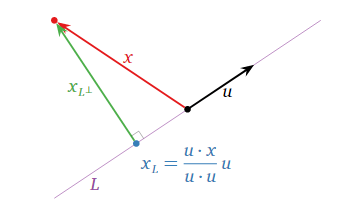
\includegraphics[width=0.3\textwidth]{Orthogonal_projection_1}
    \caption{orthogonal projection onto a line}
    \label{fig:plot_1}
\end{figure}
The vector $x_L$ is a multiple of $u$, say $x_L = cu$. This multiple is chosen so that 
\begin{align*}
    ((x - cu), u) = 0,
\end{align*}
and hence,
\begin{align*}
    c = \frac{(u, x)}{(u, u)}.
\end{align*}
The above picture\footnote{Picture source: \url{https://textbooks.math.gatech.edu/ila/projections.html}} shows the orthogonal projection in $\mathbb{R}^2$.
\end{example}

\medskip

\begin{theorem}
Let $A$ be an $m \times n$ matrix and its columns $a_1, a_2, \cdots, a_n$. Let $W = {\rm span}\{a_i\}$ and let $x$ be a vector in $\mathbb{R}^m$. Then the matrix equation
\begin{align*}
    A^T Ac = A^T x,
\end{align*}
in the unknown vector $c$ is consistent, and $x_W$ is equal to $Ac$ for any solution $c$.
\end{theorem}

\medskip

\section{Adjoint}

Let $X,U$ be two Euclidean spaces and $A:X\to U$ is a linear map, then we can define its transpose $A':U'\to X'$ defined as follows, for any $l\in U'$:
$$(A' l, x) = (l, Ax).$$
We can identify $U'$ with $U$, $X'$ with $X$.

\begin{definition}
The transpose of a map $A$ of Euclidean space $X$ into $U$ is called the adjoint of $A$, denoted by $A^*:U\to X$, which is defined as follows:
$$(A^* y, x) = (y, Ax).$$
\end{definition}

\medskip

\begin{theorem}\label{transpose_linear_map_theorem}
~\begin{enumerate}[label=(\alph*)]
    \item If $A,B$ are two linear maps of $X$ into $U$, then $(A+B)^* = A^* + B^*$.
    \item If $A:X\to U, C:U\to V$, then $(CA)^* = A^* C^*$.
    \item If $A$ is a bijection from $X$ onto $U$, then $\left(A^{-1}\right)^* = \left(A^*\right)^{-1}$.
    \item $\left(A^*\right)^* = A$.
\end{enumerate}
\end{theorem}
\begin{proof}
~\begin{enumerate}[label=(\alph*)]
    \item For $\forall x\in X, \forall y\in U$, we have
    \begin{align*}
        \left((A+B)^*y, x\right) & = (y, (A+B)x) \\
        & = (y, Ax + Bx) \\
        & = (y, Ax) + (y, Bx) \\
        & = (A^*y, x) + (B^*y, x) \\
        & = ((A^* + B^*)y, x).
    \end{align*}
    \item We have $CA:X\to V, (CA)^*:V\to X$, and then for $\forall z\in V, \forall x\in X$,
    \begin{align*}
        \left((CA)^*z, x\right) & = (z, (CA)x) \\
        & = (z, C(Ax)) \\
        & = (C^* z, Ax) \\
        & = (A^* C^* z, x).
    \end{align*}
    \item Claim $I^* = I$, and $I = A^{-1}A: X\to X$. Indeed,  for $\forall x_1, x_2\in X$,
    \begin{align*}
        (I^* x_1, x_2) & = (x_1, Ix_2) = (x_1, x_2) = (Ix_1, x_2).
    \end{align*}
    Then we have 
    \begin{align*}
        \left(A^{-1}A\right)^* & = A^* \left(A^{-1}\right)^* = I, \\
        \Rightarrow \left(A^*\right)^{-1} & = \left(A^{-1}\right)^*. 
    \end{align*}
    \item For $\forall x\in X$, we have
    \begin{align*}
        \left(A^{**}x, y\right) & = (x, A^*y) = (A^*y, x) = (y, Ax) = (Ax, y).
    \end{align*}
\end{enumerate}
\end{proof}

\begin{remark}
If we choose an orthogonal basis of $X$ and $U$, then $X$ and $U$ can be identified as $\mathbb{R}^m$ and $\mathbb{R}^n$. And $A:X\to U$ can be represented by a matrix $A:\mathbb{R}^m\to \mathbb{R}^n$, also $A^*:U\to A$ is represented by the transpose of $A$, denoted by $A'$.
\end{remark}

\section{Overdetermined Systems}

Consider a matrix equation
\begin{align*}
    Ax = p,
\end{align*}
where $p_1,\cdots.p_m$ are the measured values, and $A$ is an $m\times n$ matrix. We shall
consider the case where the number $m$ of measurements exceeds the number $n$ of quantities. 

\medskip

\begin{theorem}
Let $A$ be $m\times n$ matrix, $m > n$, and suppose that $A$ has only the trivial nullvector $0$. Then the vector $x$ that mninimizes $\|Ax - p\|$ is the unique solution $z$ to the equation
$$A^* A z = A^* p.$$
\end{theorem}
\begin{proof}
The equation $A^* A z = A^* p$ has a unique solution if and only if $A^* A$ is invertible. Indeed, suppose $A^* Ay = 0$ for some $y \in \mathbb{R}^n$, then 
\begin{align*}
    (A^* A y, y) & = 0, \\
    \Rightarrow (Ay, Ay) & = 0, \\
    \Rightarrow Ay & = 0.
\end{align*}
Since $A$ has only trivial nullvector, then $y = 0$, then the solution is unique.

Let $z$ be the minimizer, then we have
\begin{align*}
    Az - p \perp R_A,
\end{align*}
and for $\forall x\in\mathbb{R}^n$, $(Az - p, Ax) = 0$, which implies $(A^*Az - A^*p, x) = 0$. Thus, since it holds for all $x$, then we have $A^*Az = A^*p$.
\end{proof}

\begin{remark}
If $A$ has a nontrivial nullvector, then the minimizer cannot be unique.
\end{remark}

\medskip

\begin{theorem}
For any subspace $Y$ of $X$, $P_Y^* = P_Y$.
\end{theorem}
\begin{proof}
For $\forall x_1, x_2\in X$, we have
\begin{align*}
    (x_1, P_Y x_2) = (P_Y x_1, P_Y x_2) = (P_Y x_1, x_2).
\end{align*}
which implies $P_Y^* = P_Y$.
\end{proof}

\medskip

\section{Isometry and Orthogonal Group}

\begin{definition}
A mapping of a Euclidean space into itself is called an isometry if it preserves the distance of any paired points, i.e., for any $x, y\in X$, then 
\begin{align*}
    \left\|M(x) - M(y)\right\|= \|x - y\|.
\end{align*}
\end{definition}

\medskip

\begin{theorem}\label{isometry_properties}
Let $M$ be an isometry from $X$ into itself and $M(0) = 0$. Then:
\begin{enumerate}[label=(\alph*)]
    \item $M$ is linear.
    \item $M^* M = I$ and $\det M = \pm 1$.
    \item $M$ is invertible and its inverse is an isometry.
\end{enumerate}
\end{theorem}
\begin{proof}
~\begin{enumerate}[label=(\alph*)]
    \item For all $x\in X$, write $Mx = x'$, and then $\left\|x\right\|= \|x'\|$. And for any $x,y\in X$, we have $\|x' - y'\|^2 = \|x - y\|^2$. Then we have
    \begin{align*}
        \|x'\|^2 - 2(x', y') + \|y'\|^2 & = \|x\|^2 - 2(x, y) + \|y\|^2, \\
        \Rightarrow (x', y') & = (x, y).
    \end{align*}
    
    Let $z = x + y$, then we have $\left\|z'-(x'+y')\right\| - \left\|z-(x+y)\right\| = 0$, which implies $z' = x' + y'$. Also, let $z = cy$, then we have
    \begin{align*}
        \|z' - cy'\|^2 & = (z' - cy', z' - cy') \\
        & = \|z'\|^2 - 2c (z', y') + c^2 \|y'\|^2 \\
        & = \|z\|^2 - 2c (z, y) + c^2 \|y\|^2 \\
        & = \left\|z - cy\right\|= 0,
    \end{align*}
    then $z' = cy$. Combined, we have $M$ is linear.
    \item For all $x,y\in X$, $(x,y) = (Mx, My) = (M^* M x, y)$, which implies $M^* M = I$.
    \item $M$ is an isometry, implying $M$ is invertible. And since it one-to-one, also it is onto. Then $M^{-1}$ is also isometry. Indeed, 
    \begin{align*}
        \left\|M^{-1}x - M^{-1}y\right\| = \left\|M M^{-1}x - M M^{-1}y\right\| = \|x - y\|.
    \end{align*}
\end{enumerate}
\end{proof}

\begin{remark}
Conversely, if $M:X\to X$ is a linear map such that $M^* M = I$, then $M$ preserves the distance.
\end{remark}
\begin{proof}
$\|Mx\|^2 = (Mx, Mx) = (M^* M x, x) = (x, x) = \|x\|^2$.
\end{proof}

\medskip

\begin{definition}
A matrix that maps $\mathbb{R}^n$ onto itself isometrically is called orthogonal.
\end{definition}

\medskip

\begin{proposition}[Properties of orthogonal]
A matrix $M$ is orthogonal if and only if its columns are pairwise orthogonal unit vectors.
\end{proposition}
\begin{proof}
~\begin{enumerate}[label=(\arabic*)]
    \item ($\Rightarrow$) If $M$ is orthogonal, then $M$ preserves the product $$(Me_i, Me_j) = (c_i, c_j) = (e_i,e_j) = \delta_{ij},$$ 
    where $M = (c_1,\cdots,c_n)$. Then $(c_i, c_j) = \delta_{ij}$ implies its columns are pairwise orthogonal unit vectors.
    \item ($\Leftarrow$) If $(c_i, c_j) = \delta_{ij}$ for all $1\leq i, j\leq n$, then we have $M^* M = I$ naturally. Thus, $M$ is isometry.
\end{enumerate}
\end{proof}

\medskip

\begin{proposition}
A matrix $M$ is orthogonal if and only if its rows are pairwise orthogonal unit vectors.
\end{proposition}
\begin{proof}
It is obvious since $M^* = M^{-1}$.
\end{proof}

\begin{remark}
If $M$ is orthogonal, then $M$ maps any orthogonal basis into another orthogonal basis. The inverse is also true.
\end{remark}
\begin{proof}
Suppose $u_1,\cdots,u_n$ is orthogonal basis and $v_1,\cdots,v_n$ is also orthogonal basis, and $v_k = Mu_k, 1\leq k \leq n$. Then we have
$V = (v_1,\cdots,v_n) = M (u_1,\cdots,u_n) = MU$. Thus we have $M = VU^{-1}$. Hence, $M$ is orthogonal.
\end{proof}

\medskip

\section{Norm of a Linear Map}

\begin{definition}{\rm \cite{39}}\label{matrix_norm_def}
A function $\|\cdot \|: \mathbb{C}^{n^2} \to \mathbb{R}$ is a matrix norm if for any $n \times n$ matrices $A, B \in \mathbb{C}^{n^2}$, it satisfies the following five axioms:
\begin{enumerate}[label=(\arabic*)]
    \item Nonnegative, i.e., $\left\|A\right\| \geq 0$.
    
    \item Positive definite, i.e., $\left\|A\right\| = 0$ if and only if $A = 0$.
    
    \item Homogeneous, i.e., $\left\|\alpha A\right\|= |\alpha| \cdot \|A\|$ for all $\alpha \in \mathbb{C}$.
    
    \item Triangle inequality or sub-additive, i.e., $\left\|A + B\right\| \leq \|A\| + \|B\|$.
    
    \item Submultiplicativity, i.e., $\left\|A B\right\| \leq \|A\| \cdot \|B\|$. \label{Submultiplicativity}
\end{enumerate}
\end{definition}

The first four properties of a matrix norm are identical to the axioms for a norm. A norm on matrices that does not
satisfy property \ref{Submultiplicativity} for all $A$ and $B$ is a {\em vector norm on matrices}, also called a {\em generalized matrix norm}, which is given by the following definition.

\medskip

\begin{definition}\label{vector_norm_matrix_def}
The norm of a linear map $A:X\to U$ is defined by
\begin{align*}
    \left\|A\right\| = \sup_{\|x\| = 1} \left\|Ax\right\| = \sup_{\|x\| \leq 1} \|Ax\|.
\end{align*}
This norm is a matrix norm induced by vector norms, also called operator norm. When $A$ is given by a matrix, then $\left\|A\right\|$ is the square root of the largest eigenvalue of the symmetric matrix $A^TA$, all of whose eigenvalues are nonnegative.
\end{definition}

\medskip

\begin{theorem}
Let $A$ be a linear mapping from the Euclidean space $X$ into the
Euclidean space $U$, where $\|A\|$ is its norm. Then, 
\begin{enumerate}[label=(\alph*)]
    \item For any $z\in X$, $\|Az\|\leq \left\|Az\right\|\cdot \|z\|$.
    \item $\left\|A\right\| = \sup_{\|x\| = \|z\| = 1} (x, Az)$.
\end{enumerate}
\end{theorem}
\begin{proof}
~\begin{enumerate}[label=(\alph*)]
    \item If $z = 0$, then it holds. If $z\neq 0$, then we have 
    \begin{align*}
        \left\|Az\right\| = \left\|A \frac{z}{\|z\|}\|z\|\right\| = \|z\|\cdot \left\|A \frac{z}{\|z\|}\right\| \leq \|A\|\cdot \|z\|.
    \end{align*}
    \item For any $x,z\in X$, and $\|x\| = \|z\| = 1$, then 
    \begin{align*}
        (x, Az) \leq \|x\| \cdot \left\|Az\right\| \leq \|Az\|, \\
        \Rightarrow \sup_{\|x\| = \|z\| = 1} (x, Az) \leq \|Az\|.
    \end{align*}
    
    If $\left\|A\right\| = 0$, then $\sup (x, Az) = 0$, which implies $\left\|A\right\| \leq \sup (x, Az)$. If $\left\|A\right\| \neq 0$, then for all $\varepsilon > 0$, there exists $z \in X$ and $\left\|z\right\| = 1$ such that 
    \begin{align*}
        \left\|Az\right\| \geq \|A\| - \varepsilon.
    \end{align*}
    Take $x = Az/ \|Az\|$, then we have 
    \begin{align*}
        (x, Az) = \frac{\|Az\|^2}{\|Az\|} & = \|Az\| \geq \|A\| - \varepsilon, \\
        \Rightarrow \|A\| - \varepsilon & \leq \sup_{\|x\| = \|z\| = 1} (x, Az) \\
        \xrightarrow{\varepsilon \to 0} \|A\| & \leq \sup_{\|x\| = \|z\| = 1} (x, Az).
    \end{align*}
    Thus, we have $\left\|A\right\| = \sup_{\|x\| = \|z\| = 1} (x, Az)$.
\end{enumerate}
\end{proof}

\begin{remark}
For any $1\leq i,j\leq n$, $\left|a_{ij}\right| \leq \|A\|$.
\end{remark}
\begin{proof}
With the second argument in the previous theorem, $a_{ij} = (e_i,Ae_j) \leq \|A\|$.
\end{proof}

\medskip

\begin{theorem}
~\begin{enumerate}[label=(\alph*)]
    \item For all $k\in\mathbb{R}$, $\left\|kA\right\| = |k|\cdot \|A\|$.
    \item $A,B:X\to U$, then $\left\|A + B\right\| \leq \left\|A\right\| + \left\|B\right\|$.
    \item $A:X\to U, B:U\to V$, then $\left\|BA\right\| \leq \|B\|\cdot \|A\|$.
    \item $\left\|A^*\right\| = \|A\|$.
\end{enumerate}
\end{theorem}
\begin{proof}
~\begin{enumerate}[label=(\alph*)]
    \item If $k = 0$, then it holds. If $k\neq 0$, then $\left\|kAx\right\| = |k| \cdot \|Ax\|$, which implies
    \begin{align*}
        \left\|kA\right\| = \sup_{\|x\|=1} \left\|kAx\right\| = \sup_{\|x\|=1} |k| \cdot \left\|Ax\right\| = |k|\cdot \|A\|.
    \end{align*}
    \item For any $x\in X$, and $\left\|x\right\| = 1$, we have 
    \begin{align*}
        \left\|A + B\right\| \leq \sup \left\|(A+b)x\right\| = \sup \left\|Ax + Bx\right\| \leq \sup \left\|Ax\right\| + \sup \left\|Bx\right\| = \left\|A\right\| + \left\|B\right\|.
    \end{align*}
    \item For any $x\in X$, and $\|x\| = 1$, we have 
    \begin{align*}
        \left\|BA\right\| \leq \sup \left\|BAx\right\| \leq \|B\|\cdot \left\|Ax\right\| \leq \|B\|\cdot \|A\|.
    \end{align*}
    \item $A^*:U\to X$, for all $x\in X$ and all $u\in U$, we have $(A^* u, x) = (u, Ax) = (Ax, u)$. Thus, 
    \begin{align*}
        \left\|A^*\right\| = \sup_{\|x\| = \|u\| = 1} (A^*u,x) = \sup_{\|x\| = \|u\| = 1} (Ax,u) = \|A\|.
    \end{align*}
\end{enumerate}
\end{proof}

\medskip

\begin{theorem}
Let $X$ be a finite-dimensional Euclidean space and $A:X\to X$ is an invertible linear map. Let $B:X\to X$ be linear map such that 
\begin{align*}
    \left\|B - A\right\| \leq \frac{1}{\|A^{-1}\|},
\end{align*}
then $B$ is invertible.
\end{theorem}
\begin{proof}
Let $C = A - B$, then $B = A - C = A\left(I - A^{-1}C\right)$. 

It suffices to show that $I - A^{-1}C$ is invertible. Suppose by contradiction that for some $x\neq 0$, $\left(I - A^{-1}C\right)x = 0$. Then we have
\begin{align*}
    \left\|x\right\| = \left\|A^{-1}C x\right\| \leq \left\|A^{-1}C\right\| \left\|x\right\| \leq \left\|A^{-1}\right\| \|C\| \|x\|.
\end{align*}
Since $\left\|C\right\| \leq 1 / \|A^{-1}\|$, then we have $\left\|x\right\| < \left\|x\right\|$, which is a contradiction. 

Then, $I - A^{-1}C$ is invertible, so is $B$.
\end{proof}

\begin{remark}
Invertible matrices form an open and dense set.
\end{remark}

\medskip

\section{Completeness and Local Compactness}

\begin{definition}
A sequence of vectors $\{x_n\}$ in Euclidean space $X$ converges to $x\in X$ if $\|x_k - x\| \to 0$ if $k\to \infty$. We write $\lim_{k\to\infty}x_k = x$.
\end{definition}

\medskip

\begin{theorem}\label{cauchy_sequence_eclidean_theorem}
A sequence $\{x_n\}\subset X$ is called a Cauchy sequence if $\forall \varepsilon > 0$, there exists $N > 0$,  such that for all $k, j \geq N$, $\left\|x_k - x_j\right\| < \varepsilon$. 
\begin{enumerate}[label=(\alph*)]
    \item Completeness: every Cauchy sequence in a finite-dimensional Euclidean space is convergent.
    \item Locally compactness: any bounded sequence in a finite-dimensional Euclidean space contains a convergent subsequence. 
\end{enumerate}
\end{theorem}
\begin{proof}
~\begin{enumerate}[label=(\alph*)]
    \item Let $x,y$ be two vectors in $X$, and $a_j, b_j$ are their $j$th component respectively, then 
    \begin{align*}
        \left|a_j - b_j\right| \leq \|x - y\|.
    \end{align*}
    Denote by $a_{k,j}$ the $j$th component of $x_k$. Since $\{x_k\}$ is Cauchy sequence, then the sequence $\{a_{k,j}\}$ is also a Cauchy sequence. Then $\{a_{k,j}\}$ converges to a real number $a_j$. Denote $x = (a_1, \cdots, a_n)$, then we have 
    \begin{align*}
        \left\|x_k - x\right\| = \sum^n_{j=1} \left|a_{k,j} - a_j\right|^2,
    \end{align*}
    it foolows that $\lim_{k\to\infty} x_k = x$.
    \item Since $\left|a_{k,j}\right| \leq \|x_k\|$, then $\left|a_{k,j}\right| \leq M \in\mathbb{R}$ for all $k$. Since real numbers are locally compactness, then the theorem follows.
\end{enumerate}

\end{proof}

\medskip

\begin{corollary}
$$\left\|A\right\| = \max_{\|x\| = 1} \|Ax\|.$$
\end{corollary}
\begin{proof}
We know that $\left\|A\right\| = \sup_{\|x\| = 1} \|Ax\|$, then there exists a sequence $\{x_k\}$ such that $\left\|x_k\right\| = 1$ and $\lim_{k\to\infty} \left\|Ax_k\right\| = \|A\|$. Also there exists convergent subsequence $\|x_{n_k}\|$ of $\{x_k\}$, and denote by $\lim_{k\to\infty} x_{n_k} = x$. Then, we have $\left\|x\right\| = \lim_{k\to\infty} \left\|x_{n_k}\right\| = 1$. 

Since $\lim_{k\to\infty} Ax_{n_k} = Ax$, indeed, we have
\begin{align*}
    \left\|Ax_{n_k} - Ax\right\| \leq \|A\| \cdot \left\|x_{n_k} - x\right\| \to 0,
\end{align*}
then we have 
\begin{align*}
    \left\|A\right\| = \lim_{k\to\infty} \left\|Ax_{n_k}\right\| = \|Ax\|.
\end{align*}
\end{proof}

\medskip

\begin{theorem}
Let $X$ be an Euclidean space and suppose $X$ is locally compact in the sense that any bounded sequence has a convergent subsequence. Then $X$ is of finite dimension.
\end{theorem}
\begin{proof}
Assume $\dim  X = \infty$, then there exists a sequence $\{x_k\}^\infty_{k=1}$ and any finite set of vectors are linearly independent (otherwise $X$ will be finite-dimensional). Then there exists $\{e_k\}^\infty_{k=1}$ such that $(e_i, e_j) = \delta_{ij}$. And for any $i\neq j$, we have $\|e_i - e_j\|^2  = 2$. 

Thus, $\{e_k\}^\infty_{k=1}$ has no convergent subsequence, which is a contradiction.
\end{proof}

\medskip

\begin{definition}
A sequence of linear mappings $\{A_n\}$ from $X$ to $Y$ converges to $A:X\to Y$ if $\lim_{n\to\infty} \left\|A_n - A\right\| = 0$.
\end{definition}

\medskip

\begin{theorem}
In finite-dimensional spaces, then $\lim_{n\to\infty}A_n = A$ if and only if, for all $x\in X$, $\lim_{n\to\infty} A_n x = Ax$, which is called weak convergence.
\end{theorem}
\begin{proof}
~\begin{enumerate}[label=(\arabic*)]
    \item ($\Rightarrow$) If $\lim_{n\to\infty}A_n = A$, then 
    \begin{align*}
        \left\|A_n x - Ax\right\| \leq \left\|A_n - A\right\|\cdot \left\|x\right\| \xrightarrow{n \to 0} 0.
    \end{align*}
    \item ($\Leftarrow$) 
    \begin{enumerate}[label=(\alph*)]
        \item First, we show that $\{A_n\}$ is bounded. Let $\{e_i\}$ be an orthogonal basis of $X$. For each $e_i, 1\leq i\leq \dim  X = N$, we have
        \begin{align*}
            \lim_{n\to\infty} A_n e_i = A e_i,
        \end{align*}
        then $\left\|A_n e_i\right\| \leq a_i$ for all $n$ and some $a_i \geq 0$. For any $x\in X$, $x = \sum^N_{i=1}x_i e_i$, then
        \begin{align*}
            \|A_n x\| & = \left\|\sum^N_{i=1}x_i A_n e_i\right\| \\
            & \leq \sum^N_{i=1}a_i \|x_i\| \\
            & \leq \left(\sum^N_{i=1}a_i^2\right)^{\frac{1}{2}} \cdot \left(\sum^N_{i=1}\|x_i\|^2\right)^{\frac{1}{2}} \\
            &  = \left(\sum^N_{i=1}a_i^2\right)^{\frac{1}{2}} \|x\|.
        \end{align*}
        Thus, $\left\|A_n\right\|\leq \left(\sum^N_{i=1}a_i^2\right)^{1/2}$, which implies $\{A_n\}$ is bounded.
        \item Second, we prove the convergence.
        
        Let $A:X\to Y$ be defined as $Ax = \lim_{n\to\infty}A_n x$. We claim $A$ is linear. For any $x\in X, \left\|x\right\| = 1$ and $\forall \varepsilon > 0$, there exists a sequence $\{x_k\}^{N_\varepsilon}_{k=1}$ such that $\left\|x_k\right\| = 1$ and for $1\leq k \leq N_\varepsilon$, $\left\|x_k - x\right\| \leq \varepsilon$. Thus, we have
        \begin{align*}
            \left\|A_n x_k  - Ax_k\right\| & \leq \left\|A_n x - A_n x_k\right\| + \left\|A_n x - A x\right\| + \left\|Ax_k - Ax\right\| \\
            & \leq a \left\|x - x_k\right\| + \left\|A_n x - A x\right\| + \|A\|\cdot \left\|x_k - x\right\| \\
            & \leq (a + \|A\|)\left\|x_k - x\right\| + \left\|A_n x - A x\right\| \xrightarrow{n\to\infty} 0. 
        \end{align*}
        Hence, $\lim_{n\to\infty}A_n = A$.
    \end{enumerate}
\end{enumerate}
\end{proof}

\medskip

\section{Complex Euclidean Structure}

\begin{definition}
A complex Euclidean structure over a linear space $X$ over $\mathbb{C}$ is furnished by a complex valued function, called a scalar product or inner product, denoted by $(x,y)$, such that
\begin{enumerate}[label=(\arabic*)]
    \item $(x,y)$ is linear in $x$ when $y$ is fixed.
    \item Conjuate: $(x,y) = \overline{(y,x)}$ for all $x,y\in X$.
    \item Positivity: $(x,x) > 0$ for all $x\neq 0$.
\end{enumerate}
\end{definition}
\begin{remark}
For $x$ fixed, $(x, y)$ is a skew linear function of $y$, i.e.,
\begin{align*}
    (x, \alpha y_1 + \beta y_2) & = \overline{(\alpha y_1 + \beta y_2,x)} \\
    & = \overline{(\alpha y_1,x) + (\beta y_2,x)} \\
    & = \overline{\alpha} \overline{(y_1,x)} + \overline{\beta} \overline{(y_2,x)} \\
    & = \overline{\alpha}(x, y_1) + \overline{\beta}(x, y_2).
\end{align*}
\end{remark}

\medskip

\begin{definition}
The norm of $x\in X$ is defined as: $\left\|x\right\| = \sqrt{(x,x)}$.
\end{definition}

\medskip

\begin{theorem}[Schwarz Inequality]\label{schwarz_inequality}
$$\left|(x,y)\right|\leq \|x\|\cdot \|y\|.$$
\end{theorem}
\begin{proof}
We have 
\begin{align*}
    \|x+y\|^2 & = \left\|x\right\| + (x,y) + (y,x) + \left\|y\right\|^2 \\
    & = \left\|x\right\| + 2\Re (x,y) + \left\|y\right\|^2.
\end{align*}
For any $\lambda$, $\|\lambda x + y\|^2 = \lambda^2 \|x\|^2 + 2\lambda \Re (x,y) + \|y\|^2 \geq 0$, then we have
\begin{align*}
    4\left|\Re (x,y)\right|^2 & - 4\|x\|^2 \|y\|^2 \leq 0 \\
    \Rightarrow \left|\Re (x,y)\right| & \leq \|x\|\cdot \|y\|. 
\end{align*}
Since $\left(e^{i\theta}x,y\right) = e^{i\theta}(x,y)$, then we pick $\theta$ such that $e^{i\theta}(x,y) > 0$. Thus, we have
\begin{align*}
    \left|(x,y)\right| = \left|\Re (e^{i\theta}x,y)\right| \leq \|x\|\cdot \|y\|.
\end{align*}
\end{proof}

\medskip

\begin{proof}[Second Proof of Theorem \ref{schwarz_inequality}]
If $y = 0$, then the theorem is trivially true. If $y \neq 0$, let $\lambda = (x,y) / \|y\|^2$, then
\begin{align*}
    0 & \leq \left\|x - \lambda y\right\|^2 \\
    & = \left\|x\right\|^2 - (x,\lambda y) - (\lambda y,x) + \left\|\lambda y\right\|^2 \\
    & = \left\|x\right\|^2 - \overline{\lambda} (x,y) - \lambda (y,x) + \left\|\lambda y\right\|^2 \\
    & = \left\|x\right\|^2 - \overline{\lambda} (x,y) - \lambda \overline{(x,y)} +  \lambda \overline{\lambda} \left\|y\right\|^2 \\
    & = \left\|x\right\|^2 - \frac{\left|(x,y)\right|^2}{\|y\|^2} - \frac{\left|(x,y)\right|^2}{\|y\|^2} + \frac{\left|(x,y)\right|^2}{\|y\|^2} \\
    & = \left\|x\right\|^2 - \frac{\left|(x,y)\right|^2}{\|y\|^2}.
\end{align*}
Therefore, we have
\begin{align*}
    0 \leq \left\|x\right\|^2 - \frac{\left|(x,y)\right|^2}{\|y\|^2},
\end{align*}
and thus, $\left|(x,y)\right| \leq \left\|x\right\| \left\|y\right\|$.
\end{proof}

\medskip

\begin{theorem}[Triangle Inequality]
$$\left\|x+y\right\| \leq \left\|x\right\| + \left\|y\right\|.$$
\end{theorem}
\begin{proof}
We have
\begin{align*}
    \left\|x+y\right\|^2 & = \left\|x\right\| + 2 \Re(x,y) + \left\|y\right\|^2 \\
    & \leq \left\|x\right\| + 2\left|(x,y)\right| + \left\|y\right\|^2 \\
    & \leq \left\|x\right\| + 2 \left\|x\right\| \cdot \left\|y\right\| + \left\|y\right\|^2 \\
    & = (\left\|x\right\| + \left\|y\right\|)^2.
\end{align*}
\end{proof}

\medskip

Let $X, Y$ be two complex Euclidean spaces and $AX\to Y$. The adjoint $A^*$ of $A$ is defined as follows 
\begin{align*}
    (x, A^* y) = (Ax, y),
\end{align*}
then $A^* = \overline{A^T}$ as matrix. Fix $y$, $(Ax, y)$ is linear in $X$. We claim that there exists $z\in X$ such that $(x,z) = (Ax, y)$, then $A^* y = z$. Indeed, we define in $\mathbb{C}^n$:
\begin{align*}
    (x,y) = \left((x_1,\cdots,x_n), (y_1,\cdots,y_n)\right) = \sum^n_{i=1}x_i \overline{y_i}.
\end{align*}
Then, for $A = (a_{ij})_{n\times n}:\mathbb{C}^n \to \mathbb{C}^n$, we have
\begin{align*}
    (Ax, y) & = \sum_{1\leq i,j\leq n}a_{ij} x_j \overline{y_j} \\
    & = \sum_{1\leq i,j\leq n}a_{ij} \overline{\overline{a_{ij}} y_i} \\
    & = (x, A^* y).
\end{align*}

\medskip

\begin{definition}
A linear mapping of a complex Euclidean space into itself is called unitary if it is isometry.
\end{definition}

\medskip

\begin{theorem}
$M$ is unitary if and only if $M^*M = 1$. Hence, for a unitary map $M$, $$\left|\det M\right| = 1.$$
\end{theorem}
\begin{proof}
~\begin{enumerate}[label=(\arabic*)]
    \item ($\Rightarrow$) Since $M$ is isometric, then we have $(x,y) = (Mx, My) = (M^* M x, y)$, which implies $M^* M = I$.
    
    Also, $\det M \det M^* = 1$ and $\det M = \det \overline{M}^T = \overline{\dim  M}$. Thus, we have $|\det M| = 1$.
    \item ($\Leftarrow$) If $M^*M = 1$, then we have
    \begin{align*}
        (x,y) = (M^* M x, y) = (Mx, My)
    \end{align*}
    which implies $M$ is isometric.
\end{enumerate}
\end{proof}

\medskip

\begin{theorem}
Let $A:\mathbb{R}^n \to \mathbb{R}^n$ or $A:\mathbb{C}^n \to \mathbb{C}^n$, then 
\begin{align*}
    \left\|A\right\| \leq \left(\sum_{1\leq i,j\leq n} \left|a_{ij}\right|^2\right)^{\frac{1}{2}}.
\end{align*}
\end{theorem}
\begin{proof}
For any $x\in \mathbb{C}^n$, we have
\begin{align*}
    \|Ax\|^2 & = \sum^n_{i=1} \left|\sum^n_{j=1}a_{ij} x_j\right|^2 \\
    & \leq \sum^n_{i=1} \left(\sum^n_{j=1}\left|a_{ij}\right|^2 \right) \left(\sum^n_{j=1} x_j^2 \right) \\
    & = \|x\| \left(\sum^n_{i=1}\sum^n_{j=1}\left|a_{ij}\right|^2 \right),
\end{align*}
then we have $\left\|A\right\|\leq \left(\sum^n_{i=1}\sum^n_{j=1}\left|a_{ij}\right|^2 \right)$.
\end{proof}

\begin{definition}
The quantity $\left(\sum^n_{i,j=1}\left|a_{ij}\right|^2 \right)^{1/2}$ is called the Hilbert-Schmidt norm of the matrix $A$, denoted by $\|A\|_{HS}$. 
\end{definition}

\begin{remark}
$\sum^n_{i,j=1}\left|a_{ij}\right|^2 = \tr A^*A = \tr AA^*$.
\end{remark}

\medskip

\section{Spectral Radius}

\begin{definition}
The spectral radius $r(A)$ of a linear mapping $A:X\to X$ is defined as
\begin{align*}
    r(A) = \max_{j} \left|\lambda_j \right|
\end{align*}
where $\lambda_j$ are all possible eigenvalues.
\end{definition}

\begin{remark}
$r(A), \|A\|, \|A\|_{HS}$ are measures of the sign of $A$.
\end{remark}

\medskip

\begin{proposition}
$\left\|A\right\| \geq r(A)$.
\end{proposition}
\begin{proof}
Let $\lambda$ be an eigenvalue of $A$ such that $r(a) = \left|\lambda\right|$. Assume $x\neq 0$, $Ax = \lambda x$, then we have $\left\|A\right\|\cdot \left\|x\right\| \geq \left\|Ax\right\| = |\lambda|\cdot \left\|x\right\|$. Thus, $\left\|A\right\| \geq r(A)$.
\end{proof}

\medskip

\begin{remark}\label{remark_792}
~\begin{enumerate}[label=(\alph*)]
    \item Take $A = \begin{pmatrix}
    0 & 1  \\
    0 & 0  
    \end{pmatrix}$, then $r(A) = 0$ and $\left\|A\right\| \neq 0$. Then we can have strictly inequality.
    \item If there exists orthogonal basis formed by eigenvectors, then $\left\|A\right\| = r(A)$.
    \begin{proof}
    Suppose $\{x_k\}$ is the orthogonal basis and $Ax_k = \lambda_k x_k$. And for any $x\in X$, $x = \sum^n_{k=1}x_k e_k$, then 
    \begin{align*}
        Ax = \sum^n_{k=1} x_k \lambda_k e_k
    \end{align*}
    where $\|x\|^2 = \sum^n_{i=1}|x_k|^2$. Then we have 
    \begin{align*}
        \|Ax\|^2 = \sum^n_{k=1} |x_k \lambda_k|^2 \leq r(A)^2 \|x\|^2. 
    \end{align*} 
    which implies 
    \begin{align*}
        \frac{\|Ax\|}{\|x\|} = \left\|A \frac{x}{\|x\|}\right\| \leq r(A).
    \end{align*}
    Since this is true for any $x$, and $\left\|A\right\| = \max_{\|x\|=1}\|Ax\|$, therefore $\left\|A\right\| \leq r(A)$. With previous proposition, we have $\left\|A\right\| = r(A)$.
    \end{proof}
\end{enumerate}
\end{remark}

\medskip

It follows from Remark \ref{remark_792}(b) that if $A$ is diagonalizable, then $\left\|A\right\| = r(A)$.

\medskip

\begin{theorem}[Gelfand's Formula]\label{Gelfand_Formula}
$$r(A) = \lim_{k\to\infty} \left(\left\|A^k\right\|\right)^{1/k}. $$
\end{theorem}
\begin{proof}
First, we need a lemma.
\begin{lemma}\label{Gelfand_Formula_lemma}
If $r(A) < 1$, then $\lim_{k\to\infty}A^k = 0$.
\end{lemma}
\begin{proof}
Let $J$ be the Jordan canonical form of $A$, then $r(A) = r(J) < 1$. And we have 
\begin{align*}
    J =  \begin{pmatrix}
    J_1 &  &  \\
     & \ddots  &  \\
     &   & J_l
    \end{pmatrix},
\end{align*}
where $$J_s = \left(\begin{smallmatrix}
    \lambda & 1 &  & \\
     & \ddots  & \ddots & \\
     &   & \ddots &  \\
     &   &   & \lambda
\end{smallmatrix}\right)_{n_s\times n_s}, 1\leq s\leq l.$$
Then we have 
\begin{align*}
    J_s^k = \begin{pmatrix}
    \lambda^k & \binom{k}{1}\lambda^{k-1} & \binom{k}{2}\lambda^{k-2} & \cdots & \binom{k}{n_s-1} \lambda^{k - n_s +1} \\
     & \ddots  & \ddots &  & \vdots \\
     &         & \ddots &  \ddots & \vdots \\
     &         &        &  \ddots & \binom{k}{1}\lambda^{k-1} \\
     &         &        &         & \lambda^k
    \end{pmatrix}.
\end{align*}
We claim $\lim_{k\to\infty}\binom{k}{j}\lambda^{k-j} = 0, 0\leq j\leq n_s-1$ for $|\lambda| < 1$. Then we have $\lim_{k\to\infty} J_s^k = 0$, which implies $\lim_{k\to\infty} J^k = 0$. Since $A = MJM^{-1}$, then $\lim_{k\to\infty} A^k = 0$.
\end{proof}

Now we complete the proof of the theorem.
\begin{enumerate}[label=(\alph*)]
    \item Since $\left\|A\right\| \geq r(A)$, then we have $\left\|A^k\right\| \geq \left(r\left(A^k\right) \right)^{\frac{1}{k}} = \left(r(A)^k \right)^{\frac{1}{k}}  = r(A)$. Then,
    \begin{align*}
        \liminf_{k\to\infty} \left(\left\|A^k\right\|\right)^{1/k} \geq r(A).
    \end{align*}
    \item Consider for any $\varepsilon > 0$ and let $A_\varepsilon = \frac{A}{\varepsilon + r(A)}$. Since $r(A_\varepsilon) < 1$, the above lemma implies that $\lim_{k\to\infty}A_\varepsilon^k = 0$ and hence $\lim_{k\to\infty}\left\|A_\varepsilon^k\right\| = 0$. In particular, there exists $K > 0$ such that for all $k \geq K$, $\left\|A_\varepsilon^k\right\| < 1$. Then, 
    \begin{align*}
        \left(\left\|A_\varepsilon^k\right\| \right)^{\frac{1}{k}} & < 1 \\
        \Rightarrow \left\|A_\varepsilon^k\right\|^{\frac{1}{k}} & < \varepsilon + r(A) \\
        \Rightarrow \limsup_{k\to\infty} \left\|A_\varepsilon^k\right\|^{\frac{1}{k}} & \leq \varepsilon + r(A)
    \end{align*}
    Thus, as $\varepsilon \to 0$, we have $\limsup_{k\to\infty} \left\|A_\varepsilon^k\right\|^{\frac{1}{k}} \leq r(A)$.
\end{enumerate}
Combined results above gives us $r(A) = \lim_{k\to\infty} \left(\left\|A^k\right\|\right)^{1/k}$.
\end{proof}

\medskip

\begin{corollary}
Suppose $A_1 A_2 = A_2 A_1$, then $r(A_1 A_2) \leq r(A_1) r(A_2)$.
\end{corollary}
\begin{proof}
We can have $r(A_1 A_2) = \lim_{k\to\infty} \left\|(A_1 A_2)^k\right\|^{1/k}$, and $(A_1 A_2)^k = A_1^k A_2^k$ since they commute. Thus, 
\begin{align*}
    \left\|(A_1 A_2)^k\right\|^{1/k} \leq \left(\left\|A_1^k\right\|^{1/k} \right) \left(\left\|A_2^k\right\|^{1/k} \right),
\end{align*}
which implies $r(A_1 A_2) \leq r(A_1) r(A_2)$.
\end{proof}




\chapter{Spectral Theory of Self-Adjoint Mappings}
\section{Self-Adjoint Mapping}
\begin{definition}
A linear mapping $A$ of a linear or complex Euclidean space into itself is said to be self-adjoint if $A^* = A$.
\end{definition}

\begin{definition}
If we pick an orthogonal basis of Euclidean space, we can view $A$ as a matrix $A = (a_{ij})_{n\times n}$, then 
\begin{enumerate}[label=(\arabic*)]
    \item In real case, $A$ is symmetric if and only if $A^T = A$, i.e., $a_{ij} = a_{ji}$.
    
    $A$ is skew symmetric (or anti-symmetric) if and only if $A^T = -A$, i.e., $a_{ij} = -a_{ji}$.
    
    \item In complex case, $A$ is Hermitian if and only if $A^* = \overline{A^T} = A$ (conjugate transpose of $A$), i.e., $a_{ij} = \overline{a_{ji}}$.
    
    $A$ is skew Hermitian (or anti-Hermitian) if and only if $- A^* = - \overline{A^T} = A$, i.e., $a_{ij} = - \overline{a_{ji}}$.
\end{enumerate}
\end{definition}

\medskip

\begin{definition}
Let $M$ be an arbitrary linear mapping in a Euclidean space, we define its self-adjoint part as 
\begin{align*}
    M_s = \frac{M + M^*}{2}.
\end{align*}
\end{definition}

\medskip

\begin{theorem}\label{hermitian_eigenvalue_theorem}
A self-adjoint map $H$ of complex Euclidean space $X$ into itself has real eigenvalues and the set of eigenvectors which is formed by orthogonal basis of $X$.
\end{theorem}
\begin{proof}
We can view $H$ as a matrix. Then, we need to show that $H$ has following properties:
\begin{enumerate}[label=(\alph*)]
    \item $H$ has only real eigenvalues.
    
    \item $H$ has no generalized eigenvalues, only genuine ones.
    
    \item Eigenvectors of $H$ corresponding to different eigenvalues are orthogonal.
\end{enumerate}
Then, 
\begin{enumerate}[label=(\alph*)]
    \item All eigenvalues are real. Assume $\lambda$ is eigenvalue, such that $Hx = \lambda x$. Then we have
    \begin{align*}
        (Hx, x) & = (x, Hx), \\
        \Rightarrow (\lambda x, x) & = (x, \lambda x), \\
        \Rightarrow \lambda (x, x) & = \overline{\lambda} (x, x),
    \end{align*}
    and since $x \neq 0$, we have $\lambda = \overline{\lambda}$. Thus, $\Im \lambda = 0$, which implies $\lambda$ is real.
    \item There are no generalized eigenvectors. Suppose $x\in N_{(N - \lambda_i I)^2}$ and $\lambda = 0$ for simplicity, then $H^2 x = 0$, which implies
    \begin{align*}
        (H^2 x, x) & = 0, \\
        \Rightarrow (Hx, Hx) & = 0, \\
        \Rightarrow \|Hx\|^2 & = 0, \\
        \Rightarrow Hx & = 0.
    \end{align*}
    Hence, $x\in N_{(N - \lambda_i I)}$, and the index of $\lambda_i$ is $1$. Thus, there are no generalized eigenvectors.
    \item Eigenvectors of $H$ are orthogonal. Suppose $\lambda \neq \mu$ are two eigenvalues such that $Hx = \lambda x, Hy = \mu y$. Then we have
    \begin{align*}
        (Hx, y) & = (x, Hy), \\
        \Rightarrow (\lambda x, y) & = (x, \mu y), \\
        \Rightarrow \lambda(x, y) & = \overline{\mu} (x, y) = \mu (x, y),
    \end{align*}
    which implies $(x,y) = 0$. 
\end{enumerate}
\end{proof}

\medskip

\begin{theorem}\label{hermitian_diagonal}
Any Hermitian matrix $A$ can be diagonalized by a unitary matrix.
\end{theorem}
\begin{proof}
Let $\{x_k\}^n_{k=1}$ be the orthogonal basis consisting of eigenvectors of $A$, such that $Ax_k = \lambda_k x_k$, and $\lambda_k$ is real. Let $U = (x_1, x_2,\cdots, x_n)$, which is unitary, then we have 
\begin{align*}
    AU = U \begin{pmatrix}
    \lambda_1 &  &  \\
     & \ddots  &  \\
     &   & \lambda_n
    \end{pmatrix},
\end{align*}
which implies $A = U\Lambda U^{-1}$.
\end{proof}

\medskip

\begin{corollary}\label{self-adjoint-diagonal}
Any real self-adjoint matrix $H$ can be diagonalized by an orthogonal matrix, i.e. there is an orthognal matrix $M$ such that 
\begin{align*}
    M^* H M = D,
\end{align*}
where $D$ is a diagonal matrix whose entries are the eigenvalues of $H$. $M$ satisfies $M^*M = I$.
\end{corollary}
\begin{proof}
The eigenvectors $v$ of $H$ satisfies 
\begin{align}\label{equ_eigenvalue}
    Hv = \lambda v.
\end{align}
$H$ is a real self-adjoint matrix, then with part (a) in Theorem \ref{hermitian_eigenvalue_theorem}, the eigenvalues of $H$ are real. It follows from (\ref{equ_eigenvalue}) that the real and imaginary parts of $v$ are also eigenvectors. Then we can choose an orthogonal basis consisting of real eigenvectors in each eigenapsce $N_\alpha$. Since by part (iii) in Theorem \ref{hermitian_eigenvalue_theorem}, eigenvectors corresponding to disctint eigenvalues are orthogonal, we have an orthogonal basis of $X$ consisting of real eivenvectors $v_j$ of $H$. Every vector $y$ in $X$ can be expressed as
\begin{align}\label{orthogonal_basis_express}
    y = \sum^n_{j=1} z_i v_i.
\end{align}
For real $y$, then $z_i$ are real. We denote the vector with components $z_j$ as $z = \left(z_1, \cdots, z_n\right)$. Since $\{v_i\}$ form an orthogonal basis, 
\begin{align}\label{orthogonal_basis_norm}
    \|y\|^2 = \sum^n_{j=1} z_j^2 = \|z\|^2.
\end{align}
Applying $H$ to (\ref{orthogonal_basis_express}), we have \begin{align*}
    Hy = \sum^n_{j=1} z_j \lambda_j v_j.
\end{align*}
Also, setting (\ref{equ_eigenvalue}) and (\ref{orthogonal_basis_norm}) into quadratic forms $q(y) = \sum_{i,j}h_{ij} y_i y_j$ gives
\begin{align}\label{quadrtic_form}
    q(y) = (y, Hy) = \sum^n_{j=1} \lambda_j z_j^2
\end{align} 
This shows that the introduction of the new variables $z$ diagonalizes the quadratic form $q$. Relation (\ref{orthogonal_basis_norm}) states that the new vector has the same length as the old. Denote by $M$ the relation of $z$ to $y$ such that $y = Mz$. Substituting this into (\ref{quadrtic_form}) gives
\begin{align*}
    q(y) = (y, Hy) = (Mz, HMz) = (z, M^*HMz).
\end{align*}
Using (\ref{quadrtic_form}), we conclude that $M^*HM = D$.
\end{proof}

\medskip


\begin{remark}
With the theorem above, $X = \bigoplus_{\lambda_i}N_{(H-\lambda_i I)}$. We can pick orthogonal basis for $N_{(H-\lambda_i I)}$ for each $\lambda_i$, then we get orthogonal basis.
\end{remark}

\medskip

\begin{theorem}\label{theorem_symmetric}
A self-adjoint map $H$ of real Euclidean space $X$ into itself has real eigenvalues and a set of eigenvectors which is formed by orthogonal basis of $X$.
\end{theorem}
\begin{proof}
We pick an orthogonal basis of $X$ and $H$ can be represented by a matrix $A$ if we identify $X$ as $\mathbb{R}^n$, then we have $A^T = A$. We can extend $A$ to a map from $\mathbb{C}^n$ to $\mathbb{C}^n$, denoted by $\widetilde{A}$, then $\widetilde{A}^* = \widetilde{A}$. Then $\widetilde{A}$ is Hermitian matrix and we can apply the Theorem \ref{hermitian_eigenvalue_theorem}.

We claim $\sigma(A) = \sigma \left(\widetilde{A}\right)$ and $$N_{(A - \lambda I)} = \Re N_{\left(\widetilde{A} - \lambda I\right)}.$$
Indeed, $\widetilde{A}$ can be diagonalized by a unitary matrix $U$ such that $A = U\Lambda U^{-1}$, where $\Lambda$ is a real diagonal matrix. Then, $A$ can be diagonalized by a real matrix $M$ such that $A = M\Lambda M^{-1}$. Thus, the eigenvalues of $A$ are all real. Ans since
\begin{align*}
    \dim \,_{\mathbb{R}} N_{(A - \lambda I)} = \dim \,_{\mathbb{C}} N_{\left(\widetilde{A} - \lambda I\right)},
\end{align*}
we have 
\begin{align*}
    \mathbb{R}^n = \bigoplus_{\lambda \in \sigma(A)} N_{(A - \lambda I)}.
\end{align*}
Thus, we can find a set of eigenvectors that form an orthogonal basis of $\mathbb{R}^n$.
\end{proof}


\medskip

\section{Quadratic Forms}
Consider a quadratic form
\begin{align*}
    q(y) = \sum^n_{i,j=1} h_{ij} y_i y_j = (y, Hy),
\end{align*}
where $y = (y_1, \cdots, y_n)^T \in \mathbb{R}^n$, and $H = (h_{ij})_{n\times n}$ is symmetric. Let $x = Ly$, then $y = L^{-1}x$ and
\begin{align*}
    q(y) & = \left(L^{-1}x, H L^{-1}x\right) \\
    & = \left(x, \left(L^{-1}\right)^T H L^{-1}x\right) \\
    & = (x, Mx).
\end{align*}

\medskip

\begin{definition}
Two symmetric matrices $A$ and $B$ are called congruent if there exists an invertible matrix $S$ such that $A = S^T B S$.
\end{definition}

\medskip

\begin{theorem}
Given $q(x) = (x, Ax)$, there exists an invertible matrix $L$, such that
\begin{align*}
    q\left(L^{-1}x\right) = \sum^n_{i=1} d_i x_i^2,
\end{align*}
for some constants $d_i$, and we can make $d_i = 0$ or $d_i = \pm 1$.
\end{theorem}
\begin{proof}
Since $A$ is self-adjoint, then there exists a unitary matrix $Q$ such that $A = Q\Lambda Q^*$, where 
\begin{align*}
    \Lambda = \begin{pmatrix}
    \lambda_1 &  &  \\
     & \ddots  &  \\
     &   & \lambda_n
    \end{pmatrix},
\end{align*}
where $\lambda_k, 1\leq k \leq n$ are real eigenvalues of $A$. Then, we have
\begin{align*}
    q(x) & = (x, Ax) = (x, Q\Lambda Q^* x) = (Q^* x, \Lambda Q^* x), \\
    \Rightarrow q(Qx) & = (Q^* Q x, \Lambda Q^* Q x) = (Ix, \Lambda I x) = (x, \Lambda x) = \sum^n_{i=1} \lambda_i x_i^2,
\end{align*}
and we can pick $L = Q^{-1} = Q^*$. Thus the proof is complete.
\end{proof}

\medskip

\section{Law of Inertia}
\begin{theorem}[Sylvester’s Law of Inertia]\label{Law_of_Inertia}
Let $H$ be symmetric, $q(x) = (x, Hx)$ and $L$ be an invertible matrix such that
\begin{align*}
    q\left(L^{-1}x\right) = \sum^n_{i=1} d_i x_i^2,
\end{align*}
for some constants $d_i$. Then the numbers of positive, negative and zero terms of $d_i$ equal to the numbers of positive, negative and zero eigenvalues of $H$.
\end{theorem}
\begin{proof}
Let $p_+, p_-$ and $p_0$ be the numbers of positive, negative and zero terms of $d_i$. Let $S$ be a subspace of $\mathbb{R}^n$, we say $q > 0$ on $S$ if for all $u\in S, u\neq 0$, $q(u) > 0$.

We claim that $$p_+ = \max_{q > 0\,\, {\rm on}\,\, S} \dim  S. $$
Let $S = L^{-1}\left({\rm span}\{e_i, d_i > 0\} \right)$, then $
\dim  S = p_+, q > 0\,\, {\rm on}\,\, S$. 
\begin{enumerate}[label=(\alph*)]
    \item For $y\in S$, $y = L^{-1}x$, where $x = \sum_{d_i > 0} d_i c_i^2$, then 
    \begin{align*}
        q(y) = q\left(L^{-1}x\right) = \sum^n_{i=1} d_i x_i^2 = \sum_{d_i > 0} d_i c_i^2 \geq 0.
    \end{align*}
    Thus, we have $p_+ \leq \max \dim  S$.
    \item Let $S$ be any subspace with $\dim  S > p_+$, we claim that $q$ cannot be positive on $S$. For all $u\in S$, we have $Lu = \sum^n_{i=1}u_i e_i$. 
    
    Define $pu = L^{-1}\left(\sum_{d_i>0}u_i e_i \right)$, which is a projection. Then we have
    \begin{align*}
        \dim  ps \leq p_+ < \dim  S.
    \end{align*}
    Then there exists $y\in S, y\neq 0$, such that $Lpy = 0$. Assume $L = I$, then $py = 0$, which implies $q(y) = 0$. 
\end{enumerate}
\end{proof}

\begin{remark}
Two symmetric square matrices of the same size have the same
numbers of positive, negative and zero eigenvalues if and only if they are congruent.
\end{remark}

\medskip

\section{Spectral Resolution}

\begin{definition}
The set of eigenvalues of $H$ is called the spectral of $H$.
\end{definition}

\medskip

Projections can be used to describe direct-sum decompositions of the space $X$\cite{33}. Let $H$ be a self-adjoint map from $X$ into $X$, then we have 
\begin{align*}
    X = \bigoplus_{\lambda_j \in \sigma(H)}N_{H - \lambda_j I}.
\end{align*}
Hence, $N(\lambda_j) = N_{H - \lambda_j I}$ are orthogonal subspaces. Let $\lambda_j, 1\leq j\leq k$ be distinct eigenvalues. For any $x\in X$, then $x$ can be represented as $x = \sum^k_{j=1}x_j$, where $x_j\in N(\lambda_j)$. We say $x_j$ is orthogonal projection of $X$ to $N(\lambda_j)$, i.e., 
\begin{align*}
    x_j = P_{N(\lambda_j)}(x).
\end{align*}
Applying $H$, we have
\begin{align*}
    Hx = \sum^k_{j=1} \lambda_j x_j.
\end{align*}
Let $P_j$ be the orthogonal projection of $X$ onto $N(\lambda_j)$, we have
\begin{align*}
    I = \sum^k_{j=1} P_j,
\end{align*}
which follows $x = \sum^k_{j=1}x_j$ and hence 
\begin{align*}
    H = \sum^k_{j=1} \lambda_j P_j.
\end{align*}

\medskip

\begin{theorem}
The operators $P_j$ have the following properties:
\begin{enumerate}[label=(\alph*)]
    \item $P_j P_k = 0$ for $j\neq k, P_j^2 = P_j$.
    \item Each $P_j$ is self-adjoint, i.e., $P_j^* = P_j$.
\end{enumerate}
\end{theorem}
\begin{proof}
~\begin{enumerate}[label=(\alph*)]
    \item For any $x\in X$, $x = \sum^k_{j=1}x_j$, where $x_j\in N(\lambda_j)$, we have $P_j P_k x = P_j x_k = 0$. Thus, $P_j P_k = 0$ for $j\neq k$.
    \item For any $x = \sum^k_{j=1}x_j \in X$ and $y = \sum^k_{j=1}y_j \in X$, where $x_j, y_j \in N(\lambda_j)$, we have
    \begin{align*}
        \left(P_j x, y\right) = \left(x_j, y\right) = \left(x_j, \sum^k_{j=1}y_j\right) = \left(x_j, y_j\right),
    \end{align*}
    where in the last step we used the fact that $N_i$ is orthogonal to $x_j$ for $i\neq j$. Similarly, we have
    \begin{align*}
        \left(x, P_j y\right) = \left(x_j, y_j\right).
    \end{align*}
    Thus, we have $P_j^* = P_j$.
\end{enumerate}
\end{proof}

\medskip

\begin{definition}
A decomposition of the form:
\begin{align*}
    I = \sum^k_{j=1} P_j,
\end{align*}
where $P_j$ is a projection, i.e., satisfies $P_j P_k = 0$ for $j\neq k, P_j^2 = P_j$ and $P_j^* = P_j$, is called a resolution of the identity. Any self-adjoint map $H$ defineds a resolution of identity.
\end{definition}

\medskip

\begin{definition}
Let $H$ be a self-adjoint map, then 
\begin{align*}
    H = \sum^k_{j=1} \lambda_j P_j
\end{align*}
is called the spectral resolution of $H$.
\end{definition}

\medskip

Given any polynomial $p$, we have
\begin{align*}
    p(H) = \sum^k_{j=1} p\left(\lambda_j\right) P_j,
\end{align*}
since $H^m = \left(\sum^k_{j=1} \lambda_j P_j\right)^m = \sum^k_{j=1} \lambda_j^m P_j^m = \sum^k_{j=1} \lambda_j^m P_j$. Move generally, given a convergent series $f(t) = \sum^\infty_{k=0} a_k t^k$, we have 
\begin{align*}
    f(H) = \sum^k_{j=1} f\left(\lambda_j\right) P_j.
\end{align*}
In particular, 
$$e^H = \sum^\infty_{m=0}\frac{H^m}{m!} = \sum^\infty_{j=1} e^{\lambda_j} P_j.$$

\medskip

\begin{theorem}
Let $H, K$ be two self-adjoint matrices that commute. Then they have a common resolution of identity $I = \sum^k_{j=1} P_j$, such that
\begin{align*}
    H = \sum^k_{j=1} \lambda_j P_j, K = \sum^k_{j=1} \mu_j P_j
\end{align*}
where $\lambda_j\in\sigma(H), \mu_j\in\sigma(K)$.
\end{theorem}
\begin{proof}
Since $X = \bigoplus^l_{j=1} N\left(\lambda_j\right)$, where $\lambda_j, 1\leq j\leq l$ are distinct eigenvalue of $H$. We claim $N\left(\lambda_j\right)$ is invariant under $K$, i.e., $K: N\left(\lambda_j\right) \to N\left(\lambda_j\right)$. 

Indeed, for any $x\in N\left(\lambda_j\right)$, $HKx = KH x = \lambda_j Kx$, which implies $Kx$ is also an eigenvector of $H$. So $k$ maps $N\left(\lambda_j\right)$ into $N\left(\lambda_j\right)$, we now apply spectral resolution of $K$ over $N\left(\lambda_j\right)$, which gives us the theorem.
\end{proof}

\medskip

\section{Anti-Self Adjoint Mappings}
\begin{definition}
A linear mapping $A$ of Euclidean space into itself is called anti-self-adjoint if $A^* = -A$.
\end{definition}
\begin{remark}
If $A$ is anti-self adjoint, then $(iA)^* = iA$. Thus $A$ can be unitary diagonalized. Also, if $A$ is anti-self adjoint, then $AA^* = A^* A$.
\end{remark}

\medskip

\begin{theorem}\label{anti_symmetric_eigenvalue}
An anti-symmetric map $A$ has all purely imaginary eigenvalues.
\end{theorem}
\begin{proof}
Assume $\lambda$ is eigenvaule, such that $Ax = \lambda x$. Since $(Ax, x) = (x, A^*x)$, then $(Ax, x) = - (x, Ax)$, which implies $(\lambda x, x) = - (x, \lambda x)$. Thus, $\lambda = - \Bar{\lambda}$ and hence $\lambda$ is purely imaginary. 
\end{proof}

\medskip

\begin{definition}
A mapping $A$ from a compact Euclidean space into itself is normal if it commutes with its adjoint operator, i.e., $AA^* = A^* A$.
\end{definition}

\medskip

\begin{theorem}
A normal map $N$ has an orthonormal basis consists of eigenvectors.
\end{theorem}
\begin{proof}
Define $H = \frac{N+N^*}{2}$ and $A = \frac{N-N^*}{2}$, then both $H$ and $A$ are self-adjoint. Then we have
\begin{align*}
    HA & = \frac{1}{4}\left(N^2 + N^*N - NN^* - \left(N^*\right)^2 \right) \\
    & = \frac{1}{4}\left(N^2 - \left(N^*\right)^2 \right)\\
    & = AH.
\end{align*}
Then there exists a basis consisting of eigenvectors for both $A$ and $H$. Then we claim that the eigenvectors of $A+H$ are equal to that of $N$, since if we have $Av = \lambda v$ and $Hv = \mu v$, then $(A+H)v = N v = (\lambda + \mu)v$.
\end{proof}

\medskip

\begin{corollary}\label{normal_matrix_unitary_diagonal}
$N$ is a normal matrix if and only if $N$ can be unitarily diagonalized.
\end{corollary}
\begin{proof}
~\begin{enumerate}[label=(\alph*)]
    \item ($\Rightarrow$) We need three steps to show this direction\cite{25}.
    \begin{enumerate}[label=\arabic**)]
        \item If a normal matrix is upper triangular, then it is diagonal.
        
        \item By Schur decomposition\footnote{Schur decomposition theorem is talked later in Theorem \ref{Schur_Decomposition}.}, every matrix is unitary similar to an upper triangular matrix.
        
        \item Then, $N$ is similar to an upper triangular matrix, which is necessarily diagonal.
    \end{enumerate}
    Thus, $N$ is unitarily diagonalizable. 
    
    \item ($\Leftarrow$) This direction is obvious. Suppose there exists an unitary matrix $U$ such that $N = U \Lambda U^*$, where $\Lambda$ is diagonal. Then, $N N^* = U \Lambda^2 U^* = N^* N$. Thus, $N$ is normal.
\end{enumerate}
\end{proof}

\medskip

\begin{theorem}\label{isometry_property}
Let $U$ be a unitary map of a complex Euclidean space into itself, that is an isometry linear map. Then,
\begin{enumerate}[label=(\alph*)]
    \item There is an orthogonal basis consisting of genuine eigenvectors of $U$.
    \item The eigenvalues of $U$ are complex numbers with absolute value $1$.
\end{enumerate}
\end{theorem}
\begin{proof}
~\begin{enumerate}[label=(\alph*)]
    \item Since $U$ is unitray, i.e., $UU^* = U^*U = I$, then $U$ is self-adjoint, which implies $U$ is normal. Thus,  the previous theorem indicates the argument.
    \item Isometry preserves the distance, then 
    \begin{align*}
        \left\|Ux\right\| = |\lambda| \left\|x\right\| = \left\|x\right\|.
    \end{align*}
    Thus, $\left|\lambda\right| = 1$.
\end{enumerate}
\end{proof}

\medskip

\section{Rayleigh Quotient}

\begin{definition}
Let $H$ be self-adjoint, then the quotient
\begin{align*}
    R_H(x) = \frac{(x,Hx)}{(x,x)}
\end{align*}
is called the Rayleigh quotient of $H$.
\end{definition}

\begin{remark}
~\begin{enumerate}[label=(\arabic*)]
    \item $R_H(kx) = R_H(x)$.
    \item $R_H(x)$ is continuous and real valued, thus it has maximum and minimum.
\end{enumerate}
\end{remark}

\medskip

\begin{theorem}
Maximum and minimum of $R_H(x)$ are eigenvalues of $H$.
\end{theorem}
\begin{proof}
We can view $R_H$ as a real continuous map on the unit sphere. Hence, $R_H$ has a maximum and a minimum. Let $\left\|x\right\| =1$, then for any $y$, we have 
\begin{align*}
    R_H(x) = \max_{\|y\|=1} \frac{(y,Hy)}{(y,y)}.
\end{align*}
then we have $\dv{R_H(x+ty)}{t}\bigg|_{t = 0} = 0$. Also, we have
\begin{align*}
    \dv{R_H(x+ty)}{t}\bigg|_{t = 0} & = \dv{}{t}\bigg|_{t = 0} \frac{(x,Hx) + 2t\Re (x,Hy) + t^2 (y,Hy)}{\|x\|^2 + 2t \Re (x,y) + t^2 \|y\|^2} \\
    & = \frac{2\Re (x,Hy)}{\|x\|^2} - \frac{(x,Hx) 2 \Re (x,y)}{\|x\|^4} \\
    & = 2\Re (x,Hy) - (x,Hx) 2 \Re (x,y) \\
    \Rightarrow \Re (Hx,y) & =  \Re ((x,Hx)x,y)
\end{align*}
which implies $Hx = (x,Hx)x$. Thus, $x$ is an eigenvector, and $(x,Hx) = R_H(x), \left\|x\right\| = 1$ is an eigenvalue.
\end{proof}

\medskip

\begin{corollary}
\begin{align*}
    \max_{x\neq 0}R_H(x) & = \max_{\lambda\in \sigma(H)}\lambda \\
    \min_{x\neq 0}R_H(x) & = \min_{\lambda\in \sigma(H)}\lambda.
\end{align*}
\end{corollary}

\begin{remark}
Every eigenvector $x$ of $H$ is a critical point of $R_H$, that is, the first derivative of $R_H$ are zero when $x$ is an eigenvector of $H$. Conversely, the eigenvectors are the only critical points of $R_H(x)$. The value of the Rayleigh quotient at an eigenvector is the corresponding eigenvalue of $H$.
\end{remark}

\medskip

\section{Minimax Principle}

\begin{theorem}\label{minimax_principle}
Let $H$ be a self-adjoint map of a Euclidean space $X$ of finite dimension. Denote the eigenvalues of $H$, arranged in increasing order by $\lambda_1 \leq \lambda_2 \leq \cdots \leq \lambda_n$. Then,
\begin{align*}
    \lambda_j = \min_{\dim  S=j} \left\{ \max_{x\in S, x\neq 0} R_H(x) \right\},
\end{align*}
where $S$ is a linear subspace of $X$.
\end{theorem}
\begin{proof}
Let $\{x_j\}^n_{j=1}$ be the orthogonal basis of $X$ such that $Hx_j = \lambda_j x_j$. For any $x\in X$ and $x = \sum^n_{j=1}c_j x_j$, then 
\begin{align*}
    R_H(x) = \frac{\sum^n_{j=1}\lambda_j |c_j|^2}{\sum^n_{j=1} |c_j|^2}.
\end{align*}
Let $S_j = {\rm span} \{x_1,\cdots,x_j\}$, then 
\begin{align*}
    \max_{x\in S_j, x\neq 0} R_H(x) = \max \frac{\sum^j_{k=1}\lambda_k |c_k|^2}{\sum^j_{k=1} |c_k|^2} = \lambda_j,
\end{align*}
which implies 
\begin{align*}
    \min_{\dim  S=j} \left\{ \max_{x\in S, x\neq 0} R_H(x) \right\} \leq \lambda_j.
\end{align*}

Next, given any $S$ with $\dim  S = j$, we need to show $\max_{x\in S, x\neq 0} R_H(x) \geq \lambda_j$. It suffices to show that there exists $x\in S$, such that the projection of $x$ on $S_{j-1}$ is zero. Denote the projection by $P:S_j\to S_{j-1}$, with Rank-Nullity theorem, there exists $x^* = \sum_{k\geq j}c_k x_k \in S, x^*\neq 0$ such that $Px^* = 0$. Hence, we have
\begin{align*}
    \max_{x\in S, x\neq 0} \frac{(x,Hx)}{(x,x)} \geq \frac{(x^*, Hx^*)}{(x^*,x^*)} = \frac{\sum_{k\geq j}\lambda_k |c_k|^2}{\sum_{k\geq j} |c_k|^2} \geq \lambda_j.
\end{align*}
since $S$ is arbitrary subspace of dimension $j$, then we have
\begin{align*}
    \min_{\dim  S=j} \left\{ \max_{x\in S, x\neq 0} R_H(x) \right\} \geq \lambda_j.
\end{align*}
Thus we complete the theorem.
\end{proof}

\begin{remark}
Eigenvalues $\lambda_1 \leq \cdots \leq \lambda_n$ of a self-adjoint map $H$ can also be characterized as 
\begin{align*}
    \lambda_k = \max_{\dim  S = n - k + 1} \left\{ \min_{x\in S, x\neq 0} R_H(x) \right\}.
\end{align*}
In particular, the simpler formula for the maximal and minimal eigenvalues can be given by
\begin{align*}
    \lambda_n = \max_{x \neq 0} R_H(x), \quad \lambda_1 = \min_{x \neq 0} R_H(x).
\end{align*}
\end{remark}

\medskip

\section{Generalized Rayleigh Quotient}

\begin{definition}
A self-adjoint map $M$ is called positive if for all nonzero $x\in X$, $(x, Mx) > 0$.
\end{definition}

\begin{remark}
With Minimax principle, we can know that $M$ being positive is equivalent to that all eigenvalues of $M$ are positive.
\end{remark}

Now we consider a generalization of the Rayleigh quotient: for $H^* = H, M^* = M$ and $M > 0$, 
\begin{align*}
    R_{H,M}(x) = \frac{(x,Hx)}{(x,Mx)}.
\end{align*}
Let $M = \left(\sqrt{M}\right)^2$, $\sqrt{M} > 0$ and $y = \sqrt{M} x$, then we have
\begin{align*}
    R_{H,M}(x) = \frac{(x,Hx)}{(x,Mx)} & = \frac{\left(\sqrt{M}^{-1}y, H\sqrt{M}^{-1}y\right)}{\left(\sqrt{M}^{-1}y, M\sqrt{M}^{-1}y\right)} \\
    & = \frac{\left(y,\left(\sqrt{M}^*\right)^{-1}H \sqrt{M}^{-1} y \right)}{(y,y)} = R_{\widetilde{H}}(y).
\end{align*}
Now we consider
\begin{align*}
    \dv{}{t}\bigg|_{t = 0} \frac{\left(x+ty,H(x+ty)\right)}{\left(x+ty,M(x+ty)\right)} = \frac{2\Re(x,Hy)}{(x,Mx)} - \frac{2(x,Hx)\Re(x,My)}{(x,Mx)^2} = 0,
\end{align*}
which implies 
\begin{align*}
    \Re(x,Mx)(x,Hy) & = \Re(x,Hx)(x,My) \\
    \Rightarrow \Re(x,Hy) & = \Re R_{H,M}(x) (Mx,y).
\end{align*}
If $x$ is a critical point of $R_{H,M}(x)$, then $\Re(x,Hy)  = \Re R_{H,M}(x) (Mx,y)$ for all $y\in X$. Thus, we have
\begin{align*}
    (Hx, y) = R_{H,M}(x) (Mx,y) \iff Hx = R_{H,M}(x) Mx.
\end{align*}

\medskip

\begin{theorem}
There exists a basis $\{x_1,\cdots,x_n\}$ of $X$ such that 
\begin{align*}
    Hx_j = \lambda_j M x_j, 
\end{align*}
where $\lambda_j$ is real and $\lambda_j = R_{H,M}(x_j)$. Moreover, $\left(x_i, Mx_j\right) = 0$ for $i\neq j$.
\end{theorem}

\medskip

\begin{corollary}
If $M,H$ are self-adjoint, all the eigenvalues of $M^{-1}H$ are real and $M^{-1}H$ is diagonalizable. If $H > 0$, then all the eigenvalues of $M^{-1}H$ are positive.
\end{corollary}

\medskip

\section{Norm and Eigenvalues}

We recall that $\left\|A\right\| = \max \left\|Ax\right\|, \left\|x\right\|=1$ or $\left\|A\right\| = \sup\frac{\|Ax\|}{\|x\|}$. Then we have the following theorem.

\medskip

\begin{theorem}
Suppose $N$ is a normal mapping of an Euclidean space $X$ into itself, then $\left\|N\right\| = r(N)$.
\end{theorem}
\begin{proof}
~\begin{enumerate}[label=(\alph*)]
    \item $r(N)\leq \|N\|$. Indeed, for any eigenvalue $\lambda_j$ and its corresponding eigenvector $x_j$, we have \begin{align*}
        \left\|Nx_j\right\| = |\lambda_j|\cdot \left\|x_j\right\|\leq \|N\|\cdot \|x_j\|,
    \end{align*}
    which implies $\max \lambda_j = r(N) \leq \|N\|$.
    \item Now we prove the other direction. If $N$ is normal, then there exists orthogonal basis $\{x_1,\cdots, x_n\}$ of $X$ consisting of eigenvectors of $N$, such that $Nx_j = \lambda_j x_j, 1\leq j\leq n$. For any $x\in X$, $x = \sum^n_{j=1}c_j x_j$, then we have
    \begin{align*}
        Nx = \sum^n_{j=1}c_j\lambda_j x_j.
    \end{align*}
    Thus, we have
    \begin{align*}
        \frac{\|Nx\|}{\|x\|} = \left(\frac{\sum^n_{j=1} |c_j|^2 |\lambda_j|^2}{\sum^n_{j=1} |c_j|^2}\right)^{\frac{1}{2}} \leq \max \lambda_j = r(N).
    \end{align*}
\end{enumerate}
\end{proof}

\medskip

\begin{theorem}
Let $A:X\to Y$, then $\left\|A\right\| = \sqrt{r(A^*A)}$.
\end{theorem}
\begin{proof}
~\begin{enumerate}[label=(\alph*)]
    \item $A^*A$ is normal and we have
    \begin{align*}
        \|Ax\|^2 & = (Ax, Ax) \\
        & = (x, A^*Ax) \\
        & \leq \|A^*A\|\cdot \|x\|^2 = r(A^*A) \|x\|^2
    \end{align*}
    which implies $\left\|A\right\| \leq \sqrt{r(A^*A)}$.
    \item Let $\lambda$ be an eigenvalue of $A^*A$ such that $\lambda = r(A^*A) \geq 0$ and $A^*Ax = \lambda x, x\neq 0$. Then, for eigenvector $x$, we have
    \begin{align*}
        \|Ax\|^2 & = (Ax,Ax) \\
        & = (x,A^*Ax) \\
        & = \lambda \|x\|^2 \\
        & = r(A^*A) \|x\|^2 
    \end{align*}
    which implies $\left\|A\right\| \geq r(A^*A)$. Indeed, 
    \begin{align*}
        \sqrt{r(A^*A)} = \frac{\|Ax\|}{\|x\|} \leq \|A\| = \max \frac{\|Ay\|}{\|y\|}.
    \end{align*}
\end{enumerate}
\end{proof}

\medskip

\section{Schur Decomposition}

\begin{theorem}\label{Schur_Decomposition}
Let $A$ be an $n\times n$ matrix. There exists unitary matrix $U$ such that
$$A = UTU^*$$
for some upper triangular matrix $T$.
\end{theorem}
\begin{proof}
First we pick $\lambda_1\in\sigma(A)$ and let $N_1 = N_{(A - \lambda_1 I)}$. Assume $k_1 = \dim  N_1 \geq 1$, then there exists orthogonal basis $\{x_1,\cdots,x_{k_1}\}$ for $N_1$. We can complete this basis to an orthogonal basis $\{x_1,\cdots,x_{k_1},x_{k_1+1},\cdots,x_n\}$ of $\mathbb{C}^n$. Let $U_1 = (x_1,\cdots,x_n)$, where $x_j$ is $j$th column of the matrix $U_1$, and 
\begin{align*}
    Ax_j & = \lambda_1 x_j, 1\leq j\leq k_1 \\
    Ax_j & = \sum^n_{k=1}b_{kj} \lambda_k, k_1+1\leq j\leq n. 
\end{align*}
Then we have 
\begin{align*}
    A(x_1,\cdots,x_n) & = (x_1,\cdots,x_n) \begin{pmatrix}
    \lambda_1 I_{k_1} & B_{12} \\
     & B_{22}
    \end{pmatrix},
\end{align*}
where
\begin{align*}
    \begin{pmatrix}
     B_{12} \\
     B_{22}
    \end{pmatrix} = \begin{pmatrix}
    b_{1,k_1+1} & \cdots & b_{1,n} \\
    \vdots & \ddots & \vdots \\
    b_{n,k_1+1} & \cdots & b_{n,n}
    \end{pmatrix}.
\end{align*}
Then we have 
\begin{align*}
    A = U_1 
    \begin{pmatrix}
    \lambda_1 I_{k_1} & B_{12} \\
     & B_{22}
    \end{pmatrix} U_1^*.
\end{align*}

Second, let $\lambda_2\in \sigma(B_{22})$, and $k_2 = \dim  N_2$, where $N_2 = N_{(B_{22}-\lambda_2 I)}$. Then there exists unitary matrix $U_2$ such that 
\begin{align*}
    B_{22} = U_2 \begin{pmatrix}
    \lambda_2 I_{k_2} & C_{12} \\
     & C_{22}
    \end{pmatrix} U_2^*.
\end{align*}
Continue this process and we can obtain an upper triangular matrix.
\end{proof}

\medskip

\begin{theorem}
Let $AB = BA$, then $A$ and $B$ can be simultaneously upper diagonalized by a unitary matrix.
\end{theorem}
\begin{proof}
Let $\lambda_1\in\sigma(A), N_1 = N_{(A - \lambda_1 I)}$, then we can know $N_1$ is invariant under $B$, i.e., $B:N_1\to N_1$. Then we have 
\begin{align*}
    A & = U_1 \begin{pmatrix}
    \lambda_1 I_{k_1} & A_{12} \\
     & A_{22}
    \end{pmatrix} U_1^* \\
    B & = U_1 \begin{pmatrix}
    \mu_1 I_{k_1} & B_{12} \\
     & B_{22}
    \end{pmatrix} U_1^*,
\end{align*}
and we claim $A_{22}B_{22} = B_{22}A_{22}$. Then this process can continue.
\end{proof}

\medskip

\begin{theorem}
If $AB = BA$, then $r(A+B)\leq r(A)+r(B)$.
\end{theorem}
\begin{proof}
With previous theorem, $A,B$ can be simultaneously upper diagonalized by a unitary matrix, then $A = UT_1U^*, B = UT_2U^*$, where $U_1, U_2$ are upper triangular matrix where the diagonal components are eigenvalues of $A$ and $B$. Then we have
$A+b = U(T_1+T_2)U^*$, and 
\begin{align*}
    T_1+T_2 = \begin{pmatrix}
    \lambda_1 + \mu_1 &  &  \\
     & \ddots &  \\
     &  & \lambda_n + \mu_n
    \end{pmatrix}
\end{align*}
where $\lambda_j\in\sigma(A), \mu_j\in\sigma(B)$. Thus we have
\begin{align*}
    r(A+B) = \max (\lambda_j + \mu_j) \leq \max \lambda_j + \max \mu_j = r(A)+r(B).
\end{align*}
\end{proof}

\medskip

\chapter{Calculus of Vector and Matrix Valued Functions}

\section{Convergence in Norm}

Let $A(t)$ be a matrix valued function, $t\in\mathbb{R}$ and $A(t)$ is an $m\times n$ matrix. 

\begin{definition}
We say $A(t)$ is continuous at $t_0\in I$, where $I$ is an open interval, if 
$$\lim_{t\to t_0}\left\|A(t) - A(t_0)\right\| = 0.$$
We say $A(t)$ is differentiable at $t_0\in I$, with derivative $\dot{A}(t_0) = \dv{A(t)}{t}\bigg|_{t=t_0}$, if 
$$\lim_{h\to 0}\left\|\frac{A(t_0+h) - A(t_0)}{h} - \dot{A}(t_0)\right\| = 0.$$
\end{definition}

\begin{remark}
Different norms for finite-dimensional spaces are equivalent. So
the above definition will not depend on the norm we use.
\end{remark}

\begin{remark}
Continuity and differentiability is equivalent to those of every element of $A(t)$. If $A(t) = \left(a_{ij}(t) \right)$, then $\dot{A}(t) = \left(\dv{}{t}a_{ij}(t)\right)$.
\end{remark}

\medskip

\begin{theorem}[Basic Rules of Differentiation]
~\begin{enumerate}[label=(\alph*)]
    \item $\dv{}{t} \left(A(t)+B(t)\right) = \dv{}{t}A(t) + \dv{}{t}B(t)$.
    \item $\dv{}{t} A(t)B(t) = \left(\dv{}{t} A(t)\right) B(t) + A(t) \dv{}{t} B(t)$.
    \item For $x(t),y(t) \in \mathbb{C}^n$, $\dv{}{t} \left(x(t), y(t)\right) = \left(\dv{}{t}x(t), y(t)\right) + \left(x(t), \dv{}{t} y(t) \right)$.
\end{enumerate}
\end{theorem}

\medskip

\begin{theorem}\label{derivative_inverss}
Suppose $A(t)$ is differentiable square matrix valued function and $A(t)$ is invertible, then
\begin{align*}
    \dv{}{t}A^{-1}(t) = - A^{-1} \dot{A} A^{-1}.
\end{align*}
\end{theorem}
\begin{proof}
$A(t)$ is differentiable, and $AA^{-1} = I$. Then we have
\begin{align*}
    A \dv{}{t}A^{-1} + \dot{A} A^{-1} = 0 \\
    \Rightarrow \dv{}{t}A^{-1} = - A^{-1} \dot{A} A^{-1}.
\end{align*}
\end{proof}

Let $A$ be a square matrix valued function, then in general, the chain rule does not hold, i.e., $\dv{}{t}A^2(t) = \dot{A}A + A\dot{A} \neq 2 A\dot{A}$. For $k\in \mathbb{N}$, 
\begin{align*}
    \dv{}{t}A^k(t) = \sum^k_{j=1} A^{j-1}\dot{A}A^{k-j}.
\end{align*}
If $A\dot{A} = \dot{A}A$, then 
\begin{align*}
    \dv{}{t}A^k(t) = k A^{k-1}(t)\dot{A}.
\end{align*}

\medskip

\begin{theorem}
Let $p$ be any polynomial, and $A$ be a square matrix valued function that is differentiable. 
\begin{enumerate}[label=(\alph*)]
    \item If for a particular value of $t$, $A(t)\dot{A}(t) = \dot{A}(t)A(t)$, then $$\dv{}{t}p(A) = p'(A)\dot{A}.$$
    \item Even if $A(t)$ and $\dot{A}(t)$ do not commute, chain rule of the trace remains,
    $$\dv{}{t}\tr p(A) = \tr \left(p'(A)\dot{A}\right).$$
\end{enumerate}
\end{theorem}
\begin{proof}
~\begin{enumerate}[label=(\alph*)]
    \item Suppose $A(t)\dot{A}(t) = \dot{A}(t)A(t)$, then we have
    \begin{align*}
        \dv{}{t}A^k(t) = k A^{k-1}(t)\dot{A}.
    \end{align*}
    then the argument is proved since all polynomials are combinations of powers.
    \item For nomcommuting $A$ and $\dot{A}$, we take the trace of 
    \begin{align*}
        \dv{}{t}A^k(t) = \sum^k_{j=1} A^{j-1}\dot{A}A^{k-j},
    \end{align*}
    and the trace is commutative, then we have
    \begin{align*}
        \tr \left(A^{j-1}\dot{A}A^{k-j} \right) = \tr \left(A^{k-1}\dot{A} \right).
    \end{align*}
    Thus, we have
    \begin{align*}
        \dv{}{t}\tr p(A) = \tr \left(p'(A)\dot{A}\right).
    \end{align*}
\end{enumerate}
\end{proof}

Now we extend the product rule to multilinear function $M(x_1,\cdots, x_k): \left(\mathbb{C}^n\right)^k \to \mathbb{C}$. Suppose $x_j(t), 1\leq j \leq k$ are differentiable, then 
\begin{align}
    \dv{}{t}M(x_1,\cdots, x_k) = M(\dot{x}_1,\cdots, x_k) + \cdots + M(x_1,\cdots, \dot{x}_k).
\end{align}
\begin{proof}
For $k=2$, we have
\begin{align*}
    & \frac{M(x_1(t+h), x_2(t+h)) - M(x_1(t), x_2(t))}{h} \\
    = & M\left(\frac{x_1(t+h)-x_1(t+h)}{h}, x_2(t)\right) + M\left(x_1(t),\frac{x_2(t+h)-x_2(t+h)}{h} \right) \\
    \overset{n\to 0}{=} & M(\dot{x}_1(t), x_2(t)) + M(x_1(t), \dot{x}_2(t)).
\end{align*}
\end{proof}

We can apply the above result to the determinant function $A(x_1,\cdots,x_n)$ defined before and we have
\begin{align}
    \dv{}{t}A(x_1,\cdots,x_n) = A(\dot{x}_1,\cdots, x_k) + \cdots + A(x_1,\cdots, \dot{x}_k).
\end{align}
If $A(t_0) = I$, then $x_i(t_0) = e_i$ for all $0 \leq i \leq n$, and hence
\begin{align}\label{equ_93}
    \dv{}{t} \det A(t)\bigg|_{t=t_0} = \tr \dot{A}(t_0).
\end{align}

\medskip

\begin{theorem}\label{trace_determinant}
Let $Y(t)$ be a differentiable matrix valued function, then for those $t$ such that $Y$ is invertible, then
\begin{align*}
    \dv{}{t} \log \det Y(t) = \tr \left(Y^{-1} \dot{Y}\right),
\end{align*}
which is equivalent to 
\begin{align*}
    \frac{\dv{}{t}\det Y(t)}{\det Y(t)} = \tr \left(Y^{-1} \dot{Y}\right).
\end{align*}
\end{theorem}
\begin{proof}
Fix $t_0$, and we have $Y(t) = Y(t_0) Y^{-1}(t_0) Y(t)$, which implies
\begin{align*}
    \det Y(t) = \det Y(t_0) \det (Y^{-1}(t_0) Y(t)).
\end{align*}
Thus, since $\det (Y^{-1}(t_0) Y(t_0)) = I$ and by (\ref{equ_93}), we have
\begin{align*}
    \dv{}{t}\det Y(t)\bigg|_{t=t_0} = \det Y(t_0) \tr \left(Y^{-1}(t_0) \dot{Y}(t) \right)\bigg|_{t=t_0}
\end{align*}
which proved the theorem.
\end{proof}

\medskip

\section{Matrix Exponential}

We claim that the Taylor series also holds to define $e^A$ for any square matrix $A$:
\begin{align*}
    e^A = \sum^\infty_{k=0} \frac{A^k}{k!}.
\end{align*}

\medskip

\begin{theorem}\label{matrix_exponential}
~\begin{enumerate}[label=(\alph*)]
    \item If $A,B$ are square matrices and $AB = BA$, then $$e^{A+B} = e^A e^B.$$
    \item If $A$ and $B$ do not commute, then in general $$e^{A+B} \neq e^A e^B.$$
    \item If $A(t)$ depends differentiable on $t$, then $e^{A(t)}$ is also differentiable.
    \item If at some $t$, $A(t)$ and $\dot{A}(t)$ commute, then 
    \begin{align*}
        \dv{}{t}e^{A(t)} = e^{A(t)} \dot{A}(t).
    \end{align*}
    \item If $A$ is anti-self adjoint, i.e., $A^* = -A$, then $e^A$ is unitary.\label{matrix_exponential_e}
\end{enumerate}
\end{theorem}
\begin{proof}
~\begin{enumerate}[label=(\alph*)]
    \item Since $AB = BA$, we have
    \begin{align*}
        e^{A+B} & = \sum^\infty_{k=0} \frac{(A+B)^k}{k!} \\
        & = \sum^\infty_{k=0} \sum^k_{j=0} \frac{\binom{k}{j}A^k B^{k-j}}{k!} \\
        & = \sum^\infty_{k=0} \sum^k_{j=0} \frac{A^k B^{k-j}}{j!(k-j)!} \\
        & = \sum^\infty_{k=0} \frac{A^k}{k!} \sum^\infty_{j=0} \frac{B^j}{j!} = e^A e^B.
    \end{align*}
    \setcounter{enumi}{4}
    \item Since $A^* = -A$, we have $AA^* = A^*A = - A^2$. Then we have $I  = e^0 = e^{A^* + A} = e^A e^{A^*} = e^A \left(e^A\right)^*$. Thus, $e^A$ is unitary.
\end{enumerate}
\end{proof}

\medskip

To calculate $e^A$, we could use Jordan canonical form $A = SJS^{-1}$, then we have $$e^A = Se^JS^{-1},$$
where 
$$J = \begin{pmatrix}
    J_1 &  &  \\
     & \ddots &  \\
     &  & J_K
    \end{pmatrix}, \,\, {\rm and} \,\, J_k =  \begin{pmatrix}
    \lambda_k & 1 & & \\
     & \ddots & \ddots & \\
     &  & \ddots & 1 \\
     &  &  & \lambda_k
    \end{pmatrix}_{l\times l} = \lambda_k I + N_l.$$
And we can calculate $e^J$ as 
\begin{align*}
    e^J = \begin{pmatrix}
    e^{J_1} &  &  \\
     & \ddots &  \\
     &  & e^{J_K}
    \end{pmatrix},
\end{align*}
where, with $I$ and $N_l$ commute, 
\begin{align*}
    e^{J_k} = e^{\lambda_k I + N_l} = e^{\lambda_k I}e^{N_l} = e^{\lambda_k} e^{N_l} = e^{\lambda_k} \sum^{l-1}_{j=0}\frac{N^j}{j!},
\end{align*}
where the summation only goes to $l-1$ since we can calculate 
\begin{align*}
    N_l = \begin{pmatrix}
    0 & 1 & & \\
     & \ddots & \ddots & \\
     &  & \ddots & 1 \\
     &  &  & 0
    \end{pmatrix}, N_l^2 = \begin{pmatrix}
    0 & 0 & 1 & &\\
     & \ddots & \ddots & \ddots & \\
     &  & \ddots & \ddots & 1 \\
     &  &  & \ddots & 0 \\ 
     &  &  &  &  0
    \end{pmatrix}, \cdots, N_l^{l-1} = \begin{pmatrix}
    0 & 0 & \cdots & 1 \\
     & \ddots & \ddots & \vdots \\
     &  & \ddots & 0 \\
     &  &  & 0
    \end{pmatrix}.
\end{align*}

\medskip

\begin{corollary}\label{exponential_trace_corollary}
$\det e^A = e^{\tr A}$.
\end{corollary}
\begin{proof}
With Jordan canonical form, $A = SJS^{-1}$ and $e^A = Se^JS^{-1}$. Thus, we have
\begin{align*}
    \det e^A = \det e^J = \prod^n_{j=1} e^{\lambda_j} = e^{\sum^n_{j=1}\lambda_j} = e^{\tr A}.
\end{align*}
\end{proof}

\medskip

\begin{theorem}
The eigenvalues depend continuously on the matrix in the sense: If we have $\lim_{n\to\infty}A_n = A$, then $\sigma(A_n)\to \sigma(A)$, i.e., for every $\varepsilon > 0$, there exists $N > 0$ such that for $\forall n\geq N$, all eigenvalues of $A_n$ are contained in the neighborhood of eigenvalues of $A$ with radius $\varepsilon$.
\end{theorem}
\begin{proof}
$p_\lambda(A) = \det(\lambda I - A) = 0$ and roots of polynomials depend continuous on the coefficients.
\end{proof}

\medskip

\begin{theorem}
Let $A(t)$ be differentiable. Suppose $A(0)$ has an eigenvalue $\lambda_0$ of multiplicity one. Then for $t$ small enough, $A(t)$ has an eigenvalue $\lambda(t)$ that depends differentiably on $t$ and $\lambda(0) = \lambda_0$.
\end{theorem}
\begin{proof}
Let $p(\lambda, t) = \det (\lambda I - A(t))$. The assumption that $\lambda_0$ is a simple root of $p(s,0)$ implies 
\begin{align*}
    p(\lambda_0,0) & = 0, \\
    \frac{\partial}{\partial \lambda}p(\lambda_0,0) & \neq 0,
\end{align*}
and from the implicit function theorem, the equation $p(\lambda,t) = 0$ has a solution $\lambda = \lambda(t)$ in a neighborhood of $t=0$ that depends differentiably on $t$.
\end{proof}

\medskip

\section{Simple Eigenvalues}

\begin{theorem}
Let $A(t)$ be differentiable and $\lambda(t)$ is a continuous function such that $\lambda(t)$ is an eigenvalue of $A(t)$ with multiplicity $1$. Then there exists eigenvector function $v(t)$ which depends differentiably on $t$. 
\end{theorem}
\begin{proof}
We need a lemma to prove the theorem.
\begin{lemma}
Let $A$ be an $n\times n$ matrix, $p = p_A$ be its characteristic polynomial and $\lambda$ be some simple root of $p$. Then at least one of the $(n-1)\times(n-1)$ principle minors of $A - \lambda I$ has nonzero determinant. Moreover, suppose the $i$-th principal minor of $A - \lambda I$ has nonzero determinant, then the $i$-th component of an eigenvector $v$ of $A$ corresponding to the eigenvalue $\lambda$ is nonzero.
\end{lemma}
\begin{proof}
Without losing generality, and assume $\lambda = 0$. Hence $p(0) = 0, p'(0) \neq 0$. We write $A = (c_1, \cdots, c_n)$ and denote $e_1, \cdots, e_n$ the standard unit vectors. Then we have
\begin{align*}
    s I - A = (se_1 - c_1, \cdots, se_n - c_n).
\end{align*}
Hence, we have
\begin{align*}
    p'(0) & = \sum^n_{j=1} \det (-c_1, \cdots, -c_{j-1}, e_j, -c_{j+1},\cdots, -c_n) \\
    & = (-1)^{n-1} \sum^n_{j=1} \det A_j,
\end{align*}
where $A_j$ is $j$-th principle minor of $A$. Since $p'(0) \neq 0$, then at least one of $\det A_j$ is nonzero.

Now suppose the $i$-th principal minors of $A$ has nonzero determinant. Denote by $v_i$ the eigenvector obtained by omitting $i$-th component, and by $A_i$ the $i$-th principle minor of $A$. Then $v_i$ satisfies $A_i v_i = 0$. Since $\det A_i \neq 0$, we have $v_i = 0$, and hence $v = 0$, which is the eigenvector without omitting $i$-th component. This is a contradiction.
\end{proof}

Now we prove the theorem. Suppose $\lambda(0) = 0$, and $\det A_i(0) \neq 0$. Then for any $t$ small enough, we have $\det (A_i(t) - \lambda(t)I) \neq 0$ and hence the $i$-th component of $v(t)$ is not equal to $0$. We set it to $1$ in order to normalize $v(t)$. For the remaining components, we have an inhomogeneous system of equations 
\begin{align*}
    \left(A_i(t) - \lambda(t)I \right) v_i(t) = - c_i^{(i)}(t),
\end{align*}
where $c_i^{(i)}(t)$ is the vector obtained from $i$-th column of $A_i(t) - \lambda(t)I$, $c_i$ by omitting the $i$-th component. So we have 
\begin{align*}
    v_i(t) = - \left(A_i(t) - \lambda(t)I \right)^{-1} c_i^{(i)}(t).
\end{align*}
Since all terms on the right hand side depend differentiably on $t$, so does $v_i(t)$ and $v(t)$. 
\end{proof}

Now we consider the derivative of the eigenvalue $\lambda(t)$ and the eigenvector $v(t)$ of a matrix function $A(t)$ when $\lambda(t)$ is a simple root of the characteristic polynomial of $A(t)$. We consider $Av = \lambda v$, then we differentiate with respect to $t$:
\begin{align*}
    \dot{A}v + A\dot{v} = \dot{\lambda}v + \lambda \dot{v}.
\end{align*}
Let $u$ be an eigenvector of $A^T$ such that $A^T u = \lambda u$. If $(u,v)\neq 0$, then we have
\begin{align*}
    (u,\dot{A}v) = \dot{\lambda} (u,v)\,\, \Rightarrow \,\, \dot{\lambda} = \frac{(u,\dot{A}v)}{(u,v)}.
\end{align*}

\begin{lemma}
Let $\lambda$ be an eigenvalue of $A$ with multiplicity $1$, such that $Av = \lambda v, A^Tu = \lambda u, uv \neq 0$, then $(u,v)\neq 0$.
\end{lemma}
\begin{proof}
If $(u,v) = 0$, and $u\in N_{\left(A^T - \lambda I\right)}$, then by Theorem \ref{theorem_371}, we have 
\begin{align*}
    v \in N_{\left(A^T - \lambda I\right)}^\perp = R_{\left(A - \lambda I\right)},
\end{align*}
which implies there exists $w\neq 0$, such that $(A - \lambda I)w = v$. Then $w$ is an genaralized eigenvector, which is contradicted to the fact that $\lambda$ is multiplicity $1$.
\end{proof}

\medskip


\chapter{Matrix Inequalities}\label{matrix_inequalities}

\section{Positive Self-adjoint Matrix}

\begin{definition}
A self-adjoint linear mapping $H$ is called positive if 
\begin{align*}
    (x, Hx) > 0,\,\, \text{for all} \,\, x \neq 0.
\end{align*}
We write $H > 0$. Similarly, we can define $H < 0, H \geq 0$ and $H \leq 0$.
\end{definition}

\medskip

Now we discuss some basic properties of positive mapping. 

\medskip

\begin{theorem}\label{unique_square_root}
~\begin{enumerate}[label=(\alph*)]
    \item The identity $I > 0$.
    \item If $A, B > 0$, then $A + B > 0$.
    \item If $A > 0, k > 0$, then $k A > 0$.
    \item If $H > 0$ and $Q$ is invertible, then $Q^* H Q > 0$.
    \item $H > 0$ if and only if all its eigenvalues are positive.
    \item $H > 0$, then $H$ is invertible.
    \item $H > 0$, then there exists a unique $S > 0$ such that $S^2 = H$.
\end{enumerate}
\end{theorem}
\begin{proof}
~\begin{enumerate}[label=(\alph*)]
    \setcounter{enumi}{3}
    \item $(x, Q^* H Q x) = (Qx, HQx) > 0$.
    \setcounter{enumi}{6}
    \item $H > 0$, then $H$ can be diagonalized by a unitary matrix $U$ such that $U\Lambda U^*$, where 
    \begin{align*}
        \Lambda = \begin{pmatrix}
            \lambda_1 &  &  \\
            & \ddots &  \\
            &  & \lambda_n
        \end{pmatrix}.
    \end{align*}
    Define $$S = U \begin{pmatrix}
        \sqrt{\lambda_1} &  &  \\
        & \ddots &  \\
        &  & \sqrt{\lambda_n}
    \end{pmatrix} U^*,$$ 
    then $S^2  = H$. 
        
    Now we need to prove that $S$ is unique. Suppose there exists $T$ such that $T^2 = H, T > 0$, then we have
    \begin{align*}
        (x, (S+T)(S-T)x) & = (x, (TS - ST)x) \\
        & = (x, TS x) - (x, STx) \\
        & = (Tx, Sx) - (Sx, Tx).
    \end{align*}
    Then $\Re (x, (S+T)(S-T)x) = 0$. Pick $x$ to be eigenvector of $S-T$ such that $(S-T)x = \mu x$, then we have 
    \begin{align*}
        \Re \mu (x, (S+T)x) = 0,
    \end{align*}
    which implies $\mu = 0$. Thus, all eigenvalues of $S-T$ are zero, hence $S = T$.
\end{enumerate}
\end{proof}

\medskip

\begin{proposition}
~\begin{enumerate}[label=(\alph*)]
    \item $M_1 < N_1, M_2 < N_2$, then $M_1 + M_2 < N_1 + N_2$.
    \item $L < M, M < N$, then $L < M$.
\end{enumerate}
\end{proposition}

\medskip

\begin{theorem}\label{inverse_of_positive_matrix}
If $M > N > 0$, then $0 < M^{-1} < N^{-1}$.
\end{theorem}
\begin{proof}
If $N = I, M > I$, then $M^{-1} < I$. Now turn to any matrix $N$. Let $R = \sqrt{N} > 0$, then we have $M > R^2$. Then
\begin{align*}
    R^{-1} M R & > I, \\
    \Rightarrow \left(R^{-1} M R\right)^{-1} & < I, \\
    \Rightarrow R M^{-1} R^{-1} & < I, \\
    \Rightarrow M^{-1} < \left(R^2\right)^{-1} & = N^{-1}.
\end{align*}
\end{proof}

\begin{proof}[Second Proof of Theorem \ref{inverse_of_positive_matrix}]
Define $A(t) = tM + (1-t)M$, and for any $t\in [0,1]$, $A(t) > 0$. And we have 
\begin{align*}
    \dv{}{t}A^{-1}(t) = - A^{-1} \dot{A} A^{-1} = - A^{-1} (M - N) A^{-1} < 0.
\end{align*}
Also, $A^{-1}(0) = N^{-1}$  and $A^{-1}(1) = M^{-1}$. For any $x\in \mathbb{C}^n, x\neq 0$, we have 
\begin{align*}
    \left(x, \dv{}{t}A^{-1}(t)x \right) & = \dv{}{t} \left(x, A^{-1}(t)x \right) < 0, \\
    \left(x, A^{-1}(0)x \right) & = \left(x, N^{-1}x \right), \\
    \left(x, A^{-1}(1)x \right) & = \left(x, M^{-1}x \right),
\end{align*}
then we have $\left(x, N^{-1}x \right) > \left(x, M^{-1}x \right)$. Thus, $\left(x, (N^{-1} - M^{-1})x \right) > 0$, which implies $M^{-1} < N^{-1}$.
\end{proof}

\medskip

\begin{theorem}
Let $A^* = A, B^* = B$, and $A > 0, AB + BA > 0$. Then, $B > 0$.
\end{theorem}
\begin{proof}
Define $B(t) = B + tA$, and $S(t) = AB(t) + B(t)A = AB + BA + 2t A^2 > 0$. If $B = B(0)$ is not positive, then there exists $t_0 \geq 0$ such that $B(t_0)$ is not positive while $B(t) > 0$ for all $t > t_0$. Then, $0 \in \sigma(B(t_0))$. 

Let $x \neq 0$, $B(t_0)x = 0$, then $(x, S(t_0)x) = (x, AB(t_0)x) + (x, B(t_0)Ax) = 0$. This is a contradiction.
\end{proof}

\medskip

\begin{theorem}
$M > N > 0$, then $\sqrt{M} > \sqrt{N} > 0$.
\end{theorem}
\begin{proof}
Let $A(t) = tM + (1-t)N > 0$, and $R(t) = \sqrt{A(t)} > 0$. Then we have 
\begin{align*}
    \dot{A} = \dot{R}R + R \dot{R} = M - N > 0.
\end{align*}
Hence, $\dot{R} > 0$, which implies $R(0) < R(1)$, i.e., $\sqrt{N} < \sqrt{M}$.
\end{proof}

\medskip

For any $A > 0$, we can write $A = U \Lambda U^*, \Lambda > 0$. We can define 
\begin{align*}
    \log A = U \log (\Lambda) U^*.
\end{align*}
If $\Lambda = \begin{pmatrix}
\lambda_1 &  &  \\
& \ddots &  \\
&  & \lambda_n
\end{pmatrix}$, then $\log (\Lambda) = \begin{pmatrix}
 \log \lambda_1 &  &  \\
& \ddots &  \\
&  & \log \lambda_n
\end{pmatrix}$.

\medskip

\begin{lemma}
For any $A > 0$, $$\log A = \lim_{m\to\infty} m \left(A^{\frac{1}{m}} - 1\right).$$
\end{lemma}
\begin{proof}
We need to check $\log \lambda = \lim_{m\to\infty} m \left(\lambda^{1/m} - 1\right)$ for any $\lambda > 0$. Indeed, 
\begin{align*}
    \lim_{m\to\infty} m \left(\lambda^{\frac{1}{m}} - 1\right) = \lim_{x\to 0^+} \frac{\lambda^x - 1}{x} = \lim_{x\to 0^+} \frac{\lambda^x \ln \lambda }{1} = \log \lambda. 
\end{align*}
Then we have
\begin{align*}
    m \left(A^{\frac{1}{m}} - 1\right) & = m \left( U \Lambda^{\frac{1}{m}} U^* - 1 \right) = U \left[m \left(\Lambda^{\frac{1}{m}} - 1\right)\right] U^* \\
    & = U \begin{pmatrix}
        m \left(\lambda_1^{\frac{1}{m}} - 1\right) &  & \\
        & \ddots & \\
        &  & m \left(\lambda_n^{\frac{1}{m}} - 1\right)
    \end{pmatrix} U^*,
\end{align*}
and hence 
\begin{align*}
    \lim_{m\to\infty} m \left(A^{\frac{1}{m}} - 1\right) = U \begin{pmatrix}
        \log \lambda_1 &  & \\
        & \ddots & \\
        &  & \log \lambda_n
    \end{pmatrix} U^* = \log A.
\end{align*}
\end{proof}

\medskip

\begin{theorem}
Suppose $0 < M < N$, then $\log M \leq \log N$.
\end{theorem}
\begin{proof}
It is obvious with the previous lemma.
\end{proof}

\medskip

\begin{definition}
A real-valued function $f(s)$ defined for $s > 0$ is called a monotone matrix function if all pairs of self-adjoint mappings $M, N$ satisfying $0 < M < N$, then $f(M) < f(N)$. 
\end{definition}
\begin{remark}
The functions $f(s) = - 1/s, s^{1/m}, \log s$ are monotone functions, but $f(s) = s^2$ is not.
\end{remark}

\section{Gram Matrices}
\begin{definition}
Let $f_1, \cdots, f_m$ be an ordered set of vectors in the Euclidean space. The matrix $G$ with entries 
\begin{align*}
    G_{ij} = \left(f_i, f_j\right)
\end{align*}
is called the Gram matrix of the set of vectors.
\end{definition}

\medskip

\begin{theorem}\label{gram_matrix_theorem}
~\begin{enumerate}[label=(\alph*)]
    \item Every Gram matrix is nonnegative.
    
    \item The Gram matrix of a set of linearly independent vectors is positive.
    
    \item Every positive matrix can be represented as a Gram matrix.
\end{enumerate}
\end{theorem}
\begin{proof}
~\begin{enumerate}[label=(\alph*)]
    \item For any $x = \sum x_i e_i \in X$, 
    \begin{align*}
        (x,Gx) & = \sum_{i} x_i\left(\sum_{j}G_{ij}x_j\right) \\
        & = \sum_{i,j} x_i G_{ij} x_j \\
        & = \sum_{i,j} x_i \left(f_i, f_j\right) x_j \\
        & = \left(\sum_i x_i f_i, \sum_j x_j f_j \right) \\
        & = \left\|\sum x_i f_i \right\|^2.
    \end{align*}
    Then parts (i) and (ii) follows immediately. 
    
    \setcounter{enumi}{2}
    \item Let $H = \left(h_{ij}\right)_{n \times n}$ be positive. Let $f_j = \sqrt{H} e_j$, then $\left(f_i, f_j\right) = \left(\sqrt{H} e_i, \sqrt{H} e_j\right) = h_{ij}$.\footnote{\noindent{\bf Method II:} Define on $\mathbb{C}^n$, $(x,y)_H = (x, Hy)$, and then the Gram matrix of the unit vectors $f_i = e_i$ is $\left(e_i, e_j\right)_H = \left(e_i, H e_j\right) = h_{ij}$.}
\end{enumerate}
\end{proof}

\medskip

\begin{example}
Take the Euclidean space to consist of real-valued functions on the interval $[0,1]$, with the scalar product
\begin{align*}
    (f,g) = \int^1_0 f(x)g(x)\, dx.
\end{align*}
Choose $f_j = x^{k-1}, k = 1,2,\cdots,n$. Then,
\begin{align*}
    \left(f_i, f_j\right) = \frac{1}{i + j - 1}, 
\end{align*}
and the associated Gram matrix is 
\begin{align*}
    G_{ij} = \frac{1}{i + j - 1}.
\end{align*}
\end{example}

\medskip

\section{Schur's Theorem}
\begin{definition}
Let $A, B$ be two $m \times n$ matrices. The Hadamard product of $A, B$ is defined by 
\begin{align*}
    A \odot B = \left(a_{ij} b_{ij} \right)_{m \times n}.
\end{align*}
\end{definition}

\medskip

\begin{theorem}[Schur's Theorem]\label{schur_theorem}
Let $A = \left(a_{ij}\right)_{n\times n}, B = \left(b_{ij}\right)_{n\times n}$ denote positive matrices. Then $A \odot B$ is also positive.
\end{theorem}
\begin{proof}
Suppose $a_{ij} = \left(f_i, f_j\right)$ and $b_{ij} = \left(g_i, g_j\right)$. Let $f_i = \left(f^1_i, f^2_i, \cdots, f^n_i\right)^T$ and $g_i = \left(g^1_i, g^2_i, \cdots, g^n_i\right)^T$, then
\begin{align*}
    a_{ij} = \sum^n_{k=1} f^k_i \overline{f^k_j}, \quad b_{ij} = \sum^n_{k=1} g^k_i \overline{g^k_j}.
\end{align*}
Then 
\begin{align*}
    a_{ij} b_{ij} = \sum^n_{k,l=1} f^k_i \overline{f^k_j} \cdot g^l_i \overline{g^l_j},
\end{align*}
and we define $h_i = \left(f^k_i g^l_i \right)$, then $a_{ij} b_{ij} = \left(h_i, h_j \right)$. Thus, $A \odot B$ is a Gram matrix. 

Suppose $\sum^n_{i=1} c_i h_i = 0$, then for any $k,l$ 
\begin{align*}
    \sum^n_{i=1} c_i f^k_i g^l_i = 0,
\end{align*}
which implies $c_i g^l_i = 0$ for any $i, l$. It follows that $c_i = 0$. Thus, $\{h_i\}$ are linearly independent, and hence $A \odot B$ is also positive.
\end{proof}

\medskip

\begin{theorem}
Let $A$ and $B$ denote real, self-adjoint, positive $n \times n$ matrices. Then for all $t$ between $0$ and $1$,
\begin{align*}
    \det \left(tA + (1-t)B \right) \geq (\det A)^t (\det B)^{1-t}.
\end{align*}
\end{theorem}
\begin{proof}
Since $\log$ is a monotonic function, we have the equivalent inequality:
\begin{align*}
    \log \det \left(tA + (1-t)B \right) \geq t \log (\det A) + (1-t) \log (\det B).
\end{align*}
It remains to show that $\log \det H$ is concave on the set of positive matrices. Note that a function whose {\em second derivative} is negative is concave. And we need to calculate the second derivative of the function $f(t) = \log \det (tA + (1-t)B)$ and verify that it is negative. Then, by Theorem \ref{trace_determinant},
\begin{align*}
    \dv{}{t} \log \det Y = {\rm tr} \left(Y^{-1} \dot{Y} \right).
\end{align*}
and then
\begin{align*}
    \dv{^2}{t^2} \log \det Y & = {\rm tr} \dv{}{t} \left(Y^{-1} \dot{Y} \right) \\
    & = {\rm tr} \left(- Y^{-1} \dot{Y} Y^{-1} \right) \dot{Y} \\
    & = - {\rm tr} \left(- Y^{-1} \dot{Y} \right) \leq 0,
\end{align*}
where we used $Y(t) = tA + (1-t)B, \dot{Y} = A - B$ and $\ddot{Y} = 0$. 
\end{proof}

\medskip

\begin{theorem}
The determinant of a positive matrix $H$ does not exceed the product of its diagonal elements, i.e.
\begin{align*}
    \det H \leq \prod^n_{i=1} h_{ii}.
\end{align*}
\end{theorem}
\begin{proof}
Since $H$ is positive, so are its diagonal entries \footnote{Take the vector $e_1$ from the standard basis, then $a_{11} = \left(e_1, H e_i\right) > 0$. And similar argument can be applied to $a_{22}, \cdots, a_{nn}$\cite{24}.}. Define $d_i = 1/\sqrt{h_{ii}}$ and denote by $D$ the diagonal matrix with diagonal entries $d_i$. Denote by the matrix $B$ by $B = DHD$. Then, $B$ is symmetric and positive and all its diagonal entries are $1$'s. Also,
\begin{align*}
    \det B = \det H \det D^2 = \frac{\det H}{\prod h_{ii}}.
\end{align*}
It suffices to show that $\det B \leq 1$. Let $\lambda_1, \cdots, \lambda_n$ be positive eigenvalues of $B$, then
\begin{align*}
    \det B = \prod^n_{i=1} \lambda_i \leq \left(\frac{\sum^n_{i=1}\lambda_i}{n}\right)^n = 1.
\end{align*}
Thus the theorem follows.
\end{proof}

\medskip

\begin{theorem}
Let $T$ be any $n \times n$ matrix whose columns are $c_1, \cdots, c_n$. Then the determinant of $T$ is in absolute value not greater than than the product of the length of its columns, i.e.
\begin{align*}
    \left|\det T \right| \leq \prod^n_{i=1} \left\|c_j \right\|.
\end{align*}
\end{theorem}
\begin{proof}
Define $H = T^*T$, and its diagonal elements are
\begin{align*}
    h_{ii} = \sum_j t^*_{ij}t_{ji} = \sum_j \overline{t_{ij}} t_{ji} = \sum_j \left|t_{ij}\right|^2 = \left\|c_i \right\|^2.
\end{align*}
Then,
\begin{align*}
    \left|\det T \right|^2 = \det H \leq \prod^n_{i=1} \left\|c_i \right\|^2,
\end{align*}
and hence the theorem follows.
\end{proof}

\medskip

\begin{theorem}
Let $H$ be an $n \times n$ real, symmetric, positive matrix. Then,
\begin{align*}
    \frac{\pi^{\frac{n}{2}}}{\sqrt{\det H}} = \int_{\mathbb{R}^n} e^{-(x,Hx)}\, dx.
\end{align*}
\end{theorem}
\begin{proof}
Let $y = \sqrt{H}x$, then $(x, Hx) = (y, y)$. Then,
\begin{align*}
    \int_{\mathbb{R}^n} e^{-(x,Hx)}\, dx & = \int_{\mathbb{R}^n} e^{-(y,y)} \frac{1}{\det \sqrt{H}} \, dy = \frac{\pi^{n/2}}{\sqrt{\det H}}.
\end{align*}
\end{proof}

\section{Eigenvalues}
\begin{lemma}
Let $A$ be a self-adjoint map of a Euclidean space $U$ into itself. We denote by $p_+(A)$ the number of positive eigenvalues of $A$ and denote by $p_-(A)$ the number of its negative eigenvalues. Then, 
\begin{align*}
    p_+(A) & = \text{maximum dimension of subspace S of U such that (Au, u) is positive on S}, \\
    p_-(A) & = \text{maximum dimension of subspace S of U such that (Au, u) is negative on S}.
\end{align*}
\end{lemma}
\begin{proof}
It follows from Sylvester’s Law of Inertia \ref{Law_of_Inertia} and minimax principle \ref{minimax_principle}.
\end{proof}

\medskip

\begin{theorem}\label{orthogonal_dimension}
Let $A$ be a self-adjoint map of a Euclidean space $U$ into itself and $V$ be a subspace of $U$ with $\dim  V = \dim  U - 1$. Denote by $P$ the orthogonal projection onto $V$. The $PAP$ is a self-adjoint map of $U$ into $U$ that maps $V$ into $V$, we denote by $B$ the restriction of $PAP$ to $V$, i.e. $B = PAP|_V$. Then,
\begin{align*}
    p_+(A) - 1 \leq p_+(B) \leq p_+(A), \\
    p_-(A) - 1 \leq p_-(B) \leq p_-(A).
\end{align*}
\end{theorem}
\begin{proof}
~\begin{enumerate}[label=(\alph*)]
    \item Let $T$ denote a subspace of $V$ of dimension $p_+(B)$ on which $B$ is positive, then $A > 0$ on $T$. Indeed, for any $v \in T$,
    \begin{align*}
        (v, Av) = (Pv, APv) = (v, PAPv) = (v, Bv) > 0.
    \end{align*}
    Then $p_+(B) \leq p_+(A)$.
    
    \item To estimate $p_+(B)$ from below, let $S$ be a subspace of $U$ of dimension $p_+(A)$ on which $A$ is positive. Let $T = S \cap V$, then we claim $\dim  T \geq \dim  S - 1$. Indeed, if $S$ is a subspace of $V$, then $T = S$ and $\dim  T = \dim  S$. If not, choose a basis $\{s_1, \cdots, s_k\}$ in $S$. At least one of these does not belong to $V$, say $s_1$. This means that $s_1$ has a nonzero component orthogonal to $V$. Then we can choose scalars $a_2, \cdots, a_k$ such that
    \begin{align*}
        s_2 - a_2 s_1, \cdots, s_k - a_k s_1
    \end{align*}
    belong to $V$. They are linearly independent, since $s_1, \cdots, s_k$ are linearly independent. It follows that 
    \begin{align*}
        \dim  S - 1 \leq \dim  T.
    \end{align*}
    
    We claim that $B$ is positive on $T$. Take any $v \neq 0$ in $T$, then
    \begin{align*}
        (Bv, v) = (PAPv, v) = (APv, Pv) = (Av, v),
    \end{align*}
    since $v$ belongs to $V$. Also, $v$ belongs to $S$, then $(Av, v) > 0$.
    
    Since $p_+(B)$ is defined as the dimension of the largest subspace on which $B$ is positive, then $\dim  T \leq p_+(B)$, and since $\dim  T \geq \dim  S - 1$, then $p_+(A) - 1 \leq p_+(B)$. The other inequality can be proved similarly. 
    \end{enumerate}
\end{proof}

\medskip

\section{Separation of Eigenvalues}
\begin{theorem}
Let $U, V, A$ and $B$ be as in Theorem \ref{orthogonal_dimension}. Denote the eigenvalues of $A$ as $\lambda_1, \cdots, \lambda_n$ and denote those of $B$ as $\mu_1, \cdots, \mu_{n-1}$. The eigenvalues of $B$ separate the eigenvalues of $A$:
\begin{align*}
    \lambda_1 \leq \mu_1 \leq \cdots \mu_{n-1} \leq \lambda_n.
\end{align*}
\end{theorem}

\medskip

\begin{theorem}
Let $M$ and $N$ denote self-adjoint matrix satisfying $M < N$. Denote the eigenvalues of $M$ in increasing order by $\lambda_1 \leq \cdots \leq \lambda_n$ and those of $N$ by $\mu_1 \leq \cdots \mu_n$. Then, $\lambda_j \leq \mu_j$ for $j = 1, \cdots, n$.
\end{theorem}
\begin{proof}
With minimax principle,
\begin{align*}
    \lambda_j & = \min_{\dim  S=j} \max_{x\in S, x\neq 0} \frac{(x, Mx)}{(x,x)}, \\
    \mu_j & = \min_{\dim  S=j} \max_{x\in S, x\neq 0} \frac{(x, Nx)}{(x,x)}.
\end{align*}
Let $T$ be the subspace of dimension $j$, then
\begin{align*}
    \mu_j = \max_{x\in T, x\neq 0} \frac{(x, N x)}{(x,x)} > \max_{x\in T, x\neq 0} \frac{(x, M x)}{(x,x)} = \lambda_j.
\end{align*}
Indeed, pick $x^* \neq 0, x^* \in T$ such that
\begin{align*}
    \frac{(x^*, M x^*)}{(x^*,x^*)} = \max_{x\in T} \frac{(x, M x)}{(x,x)}.
\end{align*}
Also,
\begin{align*}
    \max_{x\in T} \frac{(x, M x)}{(x,x)} \leq \frac{(x^*, N x^*)}{(x^*,x^*)} \leq \max_{x\in T} \frac{(x, Nx)}{(x,x)}.
\end{align*}
Thus, $\mu_j > \lambda_j$.
\end{proof}

\medskip

\begin{theorem}
Let $M$ and $N$ be self-adjoint matrices, $\lambda_j$ and $\mu_j$ their eigenvalues arrayed in increasing order. Then
\begin{align*}
    \left|\lambda_j - \mu_j\right| \leq \|M - N\|.
\end{align*}
\end{theorem}
\begin{proof}
Let $d = \|M - N\|$, then 
\begin{align*}
    N - dI \leq M \leq N + dI.
\end{align*}
Indeed, for any $x$,
\begin{align*}
    (x, (N - dI - M)x) = (x, (N - M)x) - d \|x\|^2 \leq \|N - M\| \|x\|^2 - d \|x\|^2 = 0.
\end{align*}
Similarly\cite{26}, 
\begin{align*}
    (x, (M - dI - N)x) = (x, (M - N)x) - d \|x\|^2 \leq \|M - N\| \|x\|^2 - d \|x\|^2 = 0.
\end{align*}
Then, $\mu_j - d \leq \lambda_j \leq \mu_j + d$. Thus, $\left|\lambda_j - \mu_j\right| \leq d$, for any $j$.
\end{proof}

\medskip

\section{Wielandt-Hoffman Theorem}
\begin{theorem}[Wielandt-Hoffman\cite{27}]
Let $M, N$ be self-adjoint $n \times n$ matrices and $\lambda_j$ and $\mu_j$ their eigenvalues arranged in increasing order. Then
\begin{align*}
    \sum^n_{j=1} \left(\lambda_j - \mu_j \right)^2 \leq \|M - N\|^2_2,
\end{align*}
where $\| \cdot \|_2$ is Hilbert-Schmidt norm.
\end{theorem}
\begin{proof}
\begin{align*}
    \|M - N\|^2_2 & = \tr (M-N)^*(M-N) = \tr (M-N)^2 \\
    & = \tr \left(M^2 - MN - NM + N^2\right) \\
    & = \tr \left(M^2\right) - 2 \tr (MN) + \tr \left(N^2\right) \\
    & = \sum^n_{j=1} \lambda_j^2 - 2 \tr (MN) + \sum^n_{j=1} \mu_j^2.
\end{align*}
Also, 
\begin{align*}
    \sum^n_{j=1} \left(\lambda_j - \mu_j \right)^2 = \sum^n_{j=1} \lambda_j^2 - 2 \sum^n_{j=1} \lambda_j \mu_j + \sum^n_{j=1} \mu_j^2.
\end{align*}
It suffices to show that $\sum^n_{j=1} \lambda_j \mu_j \geq \tr (MN)$. 
\begin{enumerate}[label=(\alph*)]
    \item If $M, N$ commutes, then $M, N$ can be diagonalized at the same time. The eigenvalues of $MN$ are $\lambda_j \widetilde{\mu_j}, 1 \leq j \leq n$, where $\widetilde{\mu_j}$ is a permutation of $\mu_j$. 
    Then, 
    \begin{align*}
        \tr (MN) = \sum^N_{j=1} \lambda_j \widetilde{\mu_j} \leq \lambda_j \mu_j,
    \end{align*}
    since if $a > c, b > d$, $(ab + cd) - (ad + cb) = (a - c)(b - d) \geq 0$.
    
    \item If $M, N$ does not commute, fix $M$ and consider all self-adjoint matrices $N$ whose eigenvalues are $\mu_1, \cdots, \mu_n$. The set $S$ of such matrices $N$ forms a bounded set in the space of all self-adjoint matrices. By compactness, there is such matrix $N \in S$ so that $\tr (MN)$ attains its maximum value. 
    
    Indeed, $S$ is compact. $S$ has bounded spectral radius, and hence bounded. Thus, 
    $$\max_{N \in S} \tr (MN)$$ 
    is well defined and such $N$ exists, denoted by $N_m$. 
    
    If $N(t)$ is a differentiable function whose values are self-adjoint matrices with eigenvalues $\mu_1, \cdots, \mu_n$ and $N(0) = N_m$, then 
    \begin{align*}
        \dv{}{t} \tr (N(t)M)\Bigg|_{t=0} = 0.
    \end{align*}
    Let $A = N_m M - M N_m$, then $A^* = - A$, and thus $e^{At}$ is a unitary matrix. Now let $N(t) = e^{At} N_m e^{-At}$, then
    \begin{align*}
        \dv{}{t} \tr (N(t)M)\Bigg|_{t=0} & = \dv{}{t} \tr \left(M e^{At} N_m e^{-At} \right)\Bigg|_{t=0} \\
        & = \tr \left(M A e^{At} N_m e^{-At} - M e^{At} N_m A e^{-At} \right)\Bigg|_{t=0} \\
        & = \tr \left(M A N_m - M N_m A \right) \\
        & = \tr \left(N_m M A - M N_m A \right)
    \end{align*}
    where in the last step we used the commutativity of trace. Then, 
    \begin{align*}
        \tr \left(N_m M A - M N_m A \right) = \tr \left(N_m M - M N_m \right) \tr (A) = \tr \left(A^2 \right) = - \tr (A^*A) \leq 0.
    \end{align*}
    Thus, $A = 0$ and hence $M, N_m$ commute. The rest is similar to part (a).
\end{enumerate}
\end{proof}

\medskip

\begin{theorem}
Denote by $\lambda_{\min}(H)$ the smallest eigenvalue of a self-adjoint mapping $H$ in a Euclidean space. Then $\lambda_{\min}(H)$ is a concave funuction of $H$, that is, for $0 \leq t \leq 1$,
\begin{align*}
    \lambda_{\min}(tL + (1-t)M) \geq t \lambda_{\min}(L) + (1-t) \lambda_{\min}(M).
\end{align*}
Similarly, $\lambda_{\max}(H)$ is a convex function of $H$, that is, for $0 \leq t \leq 1$,
\begin{align*}
    \lambda_{\max}(tL + (1-t)M) \leq t \lambda_{\max}(L) + (1-t) \lambda_{\max}(M).
\end{align*}
\end{theorem}
\begin{proof}
The smallest eigenvalue of a mapping can be characterized as a minimum:
\begin{align*}
    \lambda_{\min}(H) = \min_{\|x\|=1} (x, Hx).
\end{align*}
Let $x \neq 0$ be an unit vector such that
\begin{align*}
    \lambda_{\min}(tL + (1-t)M) & = (x, (tL+(1-t)M)x) \\
    & = t(x, Lx) + (1-t) (x, Mx) \\
    & \geq t \lambda_{\min}(L) + (1-t) \lambda_{\min}(M).
\end{align*}
Since $- \lambda_{\max}(H) = \lambda_{\min}(-H)$, the convexity of $\lambda_{\max}(H)$ follows.
\end{proof}

\medskip

\section{Matrices with Positive Self-Adjoint Part}

Every linear mapping $Z$ of a complex Euclidean space into itself can be decomposed, uniquely, as a sum of a self-adjoint mapping and an anti-self-adjoint one:
\begin{align*}
    Z = H + A,
\end{align*}
where
\begin{align*}
    H^* = H, \quad A^* = - A,
\end{align*}
are given by 
\begin{align*}
    H = \frac{Z + Z^*}{2}, \quad A = \frac{Z - Z^*}{2}.
\end{align*}

\medskip

\begin{theorem}
Suppose the self-adjoint part $Z$ is positive, i.e. $Z + Z^* > 0$. Then the eigenvalues of $Z$ have positive real part.
\end{theorem}
\begin{proof}
Using the conjugate symmetry of scalar product in a complex Euclidean space, and the definition of adjoint, we have, for any vector $h$,
\begin{align*}
    2 \Re (h, Zh) = (h, Zh) + \overline{(h, Zh)} = (h, Zh) + (Zh, h) = (h, (Z+Z^*)h) > 0
\end{align*}
Let $h$ be an eigenvector of $Z$ of norm $1$, corresponding to eigenvalue $\lambda$, such that $Zh = \lambda h$. Then $(h, Zh) = z$ has positive real part.
\end{proof}

\medskip

Let $a$ denote any complex number with positive real part, define
\begin{align*}
    w = \frac{1 - az}{1+\overline{a}z},
\end{align*}
and then $z \mapsto w$ maps the right half plane $\Re z > 0$ onto the unit disc $\left|w\right| < 1$. 

\medskip

\begin{theorem}
Let $a \in \mathbb{C}$ with $\Re a > 0$. Let $Z$ be a mapping whose self-adjoint part $Z + Z^* > 0$. Then
\begin{align*}
    W = \frac{I - aZ}{I + \overline{a}Z}
\end{align*}
is a mapping of norm less than $1$. Conversely, $\left\|W\right\| < 1$ implies that $Z + Z^* > 0$.
\end{theorem}
\begin{proof}
Suppose $Z + Z^* > 0$, then $\Re \lambda > 0$ for any eigenvalue $\lambda$ of $Z$. It follows that eigenvalues of $I + \overline{a} Z$ and $I + aZ$ are not zero, therefore $I + \overline{a} Z$ is invertible. For any vector $x$, denote $(I + \overline{a} Z)^{-1}x = y$, then \begin{align*}
    (I - aZ)y = Wx,
\end{align*}
and then 
\begin{align*}
    x = (I + \overline{a} Z)y.
\end{align*}
Thus,
\begin{align*}
    \left\|W\right\| \leq 1 & \Leftrightarrow \left\|Wx\right\| \leq \left\|x\right\| \\
    & \Leftrightarrow \left\|(I - aZ)y\right\| \leq \left\|(I + \overline{a} Z)y\right\| \\
    & \Leftrightarrow (a+\overline{a})(y,Zy) + (a+\overline{a})(Zy,y) > 0 \\
    & \Leftrightarrow (y, (Z+Z^*)y) > 0 \\
    & \Leftrightarrow Z+Z^* > 0.
\end{align*}
\end{proof}

\section{Polar Decomposition}
\begin{theorem}\label{polar_decomposition_theorem}
Let $A$ be a linear mapping of a complex Euclidean space into itself. Then $A$ can be factored as 
\begin{align}\label{polar_decomposition}
    A = RU,
\end{align}
where $R$ is a nonnegative self-adjoint mapping, and $U$ is unitary. When $A$ is invertible, $R$ is positive.
\end{theorem}
\begin{proof}
~\begin{enumerate}[label=(\alph*)]
    \item When $A$ is invertible, then so is $A^*$. For any $x \neq 0$,
    \begin{align*}
        (A A^* x, x) = (A^* x, A^* x) = \left\|A^* x\right\| > 0.
    \end{align*}
    This proves that $A A^*$ is a positive mapping. According to Theorem \ref{unique_square_root}, $A A^*$ has a unique positive square root $R$, i.e., $A A^* = R^2$. Define $U = R^{-1}A$, then $U^* = A^* R^{-1}$. Indeed, $R^{-1}$ is self-adjoint\footnote{According to Theorem \ref{gram_matrix_theorem}, every positive matrix can be represented as a Gram matrix, so it is self-adjoint.}. Then,
    \begin{align*}
        U U^* = R^{-1}A A^* R^{-1} = R^{-1} R^2 R^{-1} = I,
    \end{align*}
    which implies $U$ is unitary. By definition of $U$, $A = RU$.
    
    \item When $A$ is not invertible, $AA^*$ is a nonnegative self-adjoint map, then it has a unique nonnegative square root $R$. Therefore, 
    \begin{align}\label{equ_square_norm}
        \Vert R x \Vert^2 = (Rx, Rx) = (x, R^2 x) = (x, AA^*x) = (A^*x, A^*x) = \Vert A^*x \Vert^2.
    \end{align}
    Suppose $Rx = Ry$, then $\left\|R (x - y)\right\| = 0$, and according to (\ref{equ_square_norm}), $\left\|A^* (x - y)\right\| = 0$, therefore $A^* x = A^* y$. This shows that for any $u$ in the range of $R$, $u = Rx$, we can define $Vu$ as 
    $A^* x$ and then $V$ is isometry, therefore it can be extended to the whole space as a unitary mapping. By definition, $A^* = VR$, and then $A = RV^*$.
\end{enumerate}
\end{proof}

\medskip

\begin{proof}[Second Proof of Theorem \ref{polar_decomposition_theorem}(b)]
When $A$ is not invertible, let $A_\varepsilon = A + \varepsilon I$ be invertible, where $\varepsilon$ is arbitrary and positive. Let $R_\varepsilon = \sqrt{A_\varepsilon A_\varepsilon^*}$, and similarly, $R_\varepsilon$ is unique and positive. Define $U_\varepsilon = R_\varepsilon^{-1} A_\varepsilon$, then $A_\varepsilon = R_\varepsilon U_\varepsilon$. And $A_\varepsilon, R_\varepsilon, U_\varepsilon$ have convergent subsequences, meaning $A \gets A_\varepsilon = R_\varepsilon U_\varepsilon \to RU$.
\end{proof}

\medskip

\begin{remark}
The polar decomposition can also be defined as $A = UR$, where $U$ is unitary and $R$ is a nonnegative self-adjoint mapping.
\end{remark}

\medskip

\begin{remark}
If $A$ is invertible, then $R, U$ are uniquely determined. If $A$ is not invertible, then $U$ is not unique.
\end{remark}
\begin{proof}
~\begin{enumerate}[label=(\alph*)]
    \item Suppose $A = R_1U_1 = R_2 U_2$, where $R_1, R_2 > 0$, $U_1^* U_1 = U_2^* U_2 = I$. Also,
    \begin{align*}
        R_1 U_1 \left(R_1 U_1\right)^* = R_1 R_1^* = R_2 U_2 \left(R_2 U_2\right)^* = R_2 R_2^*.
    \end{align*}
    Then $R_1^2 = R_2^2$, and hence $R_1 = R_2$. Indeed, for any $x$, 
    \begin{align*}
        & \left(x, (R_1 + R_2)(R_1 - R_2)x\right) \\
        = & (x, R_1^2x) - (x, R_1 R_2 x) + (x, R_2 R_1 x) - (x, R_2^2x) \\
        = & (R_2 x, R_1 x) - (R_1 x, R_2 x),
    \end{align*}
    which implies $\Re\left(x, (R_1 + R_2)(R_1 - R_2)x\right) = 0$. 
    
    For any $x \neq 0$ and $\mu \in \sigma(R_1 - R_2), \mu \neq 0$ such that $(R_1 - R_2)x = \mu x$, we have
    \begin{align*}
        \Re\left(x, \mu (R_1 + R_2) x\right) = 0,
    \end{align*}
    and then $(R_1 + R_2) x = 0$. Therefore, since $R_1, R_2$ are positive, then $R_1 x = R_2 x = 0$, and then $(R_1 - R_2)x = 0$, which implies $\mu = 0$. Contradiction. Thus, $R_1 = R_2$.
    
    \item If $A$ is not invertible, without loss of generality, we could assume $A = 0$. Then, $R = 0$, and $U$ can be any unitary matrix.
\end{enumerate}
\end{proof}

\section{Singular Value Decomposition}

According to the spectral representation theorem \ref{hermitian_diagonal}, the self-adjoint map $R$ can be expressed as $R = WDW^*$, where $D$ is diagonal and $W$ is unitary. Substituting this into (\ref{polar_decomposition}) gives $A = WDW^* U$. Denote $W^*U$ by $V$, then 
\begin{align}\label{singular_value_decomposition}
    A = WDV,
\end{align}
where $W$ and $V$ are unitary and $D$ is diagonal, with nonnegative entries. Equation (\ref{singular_value_decomposition}) is called the {\em singular value decomposition} (SVD) of the mapping $A$. The diagonal entries of $D$ are called the {\em singular values} of $A$, which are the nonnegative square roots of the eigenvlaues of $AA^*$. 

\medskip

\begin{theorem}
Let $A$ be $m\times n$ matrix. Then there exists $m \times m$ unitary matrix $U$ and $n \times n$ unitary matrix $V$ such that
\begin{align*}
    A = U \Sigma V^*,
\end{align*}
where $\Sigma$ is $m \times n$ rectangular diagonal matrix with nonnegative real entries on diagonal.
\end{theorem}
\begin{proof}
~\begin{enumerate}[label=(\alph*)]
    \item If $m = n$, then it holds.
    
    \item Suppose $m > n$. Since $A^*A \geq 0$, then there exists $n \times n$ unitary matrix $V$ such that $A^*A = V D V^*$, where $D$ is $n \times n$ diagonal matrix and $D \geq 0$. For any $x \in \mathbb{C}^n$, 
    \begin{align*}
        \left\|AV x\right\|^2 & = (AVx, AVx) = (Vx, A^*AV x) = (Vx, V D V^* V x) \\
        & = (Vx, VDx) = (x, Dx) = \left\|D^{\frac{1}{2}} x\right\|^2.
    \end{align*}
    Let $U: \mathbb{C}^m \to \mathbb{C}^m$ maps $\begin{pmatrix}
        D^{1/2} \\
        0
    \end{pmatrix}_{m\times n}x$ to $AVx \in \mathbb{C}^m$, and $U$ is unitary, i.e., $U \begin{pmatrix} D^{1/2} \\ 0 \end{pmatrix}x = AVx$. Then, 
    \begin{align*}
        U \begin{pmatrix} D^{1/2} \\ 0 \end{pmatrix} = AV.
    \end{align*}
    Define $\Sigma = \begin{pmatrix} D^{1/2} \\ 0 \end{pmatrix}$, then $AV = U\Sigma$, and hence $A = U\Sigma V^*$.
\end{enumerate}
\end{proof}

\begin{remark}
The singular values of $A$, and hence $\Sigma$ is uniquely determined. 
\end{remark}

\begin{remark}
~\begin{enumerate}[label=(\arabic*)]
    \item $A^* A = V\Sigma^* U^* U\Sigma V^* = V\Sigma^* \Sigma V^*$, and the columns of $V$ are eigenvectors of $A^* A$, called the right singular vector of $A$.
    
    \item $A A^* = U\Sigma V^* V\Sigma^* U^* = U\Sigma \Sigma^* U^*$, and the columns of $U$ are eigenvectors of $A A^*$, called the left singular vector of $A$.
\end{enumerate}
\end{remark}

\medskip

To construct singular value decomposition, first compute for eigenvalues $\sigma_1^2, \sigma_2^2, \cdots, \sigma_n^2$ of $A^*A$. Let $v_1, v_2, \cdots, v_n$ be an orthogonal basis of eigenvectors of $A^*A$, since $AA^* \geq 0$. Then we have following theorem.

\medskip

\begin{theorem}{\rm \cite{28}}
Let $\sigma_1^2, \sigma_2^2, \cdots, \sigma_r^2$ be nonzero singular value of $AA^*$. Then the system 
\begin{align*}
    u_k = \frac{1}{\sigma_k} Av_k, k = 1,2,\cdots,r
\end{align*}
is an orthogonal system.
\end{theorem}
\begin{proof}
\begin{align*}
    (Av_i, Av_j) = (A^*A v_i, v_j) = \sigma_i^2 (v_i, v_j) = \begin{cases}
        0, & i \neq j, \\
        \sigma_i^2, & i = j,
    \end{cases}
\end{align*}
since $v_1, v_2, \cdots, v_n$ is an orthogonal basis.
\end{proof}

\medskip

Let $A$ be $m \times n$ real matrix. Define $\sigma(u,v) = (u, Av)$ for $u \in \mathbb{R}^m, v \in \mathbb{R}^n$.

\medskip

\begin{theorem}\label{eigenvalue_singular_value}
Let 
$$\lambda_1 = \max_{\|u\| = \|v\| = 1} \sigma(u,v) = \sigma(u_1, v_1).$$ 
Then, $\lambda_1$ is the largest singular value and $u_1, v_1$ are left and right singular vectors with respect to $\lambda_1$. Moreover,
\begin{align*}
    A v_1 = \lambda_1 u_1,\quad A^* u_1 = \lambda_1 v_1.
\end{align*}
\end{theorem}
\begin{proof}
By definition of $u_1, v_1$, then for any vector $g, h$, 
\begin{align*}
    f(s,t) = \frac{\sigma(u_1+sg, v_1+th)}{\|u_1+sg\| \cdot \|v_1+th\|}
\end{align*}
attains maximum at $(0,0)$. Then,
\begin{align*}
    0 = \frac{\partial f}{\partial s}\Bigg|_{(0,0)} & = \frac{\sigma(g,v_1+th)\|u_1+sg\| \cdot \|v_1+th\| - \sigma(u_1+sg, v_1+th)\frac{\|v_1+th\|}{\|u_1+sg\|}[(u_1,g) + (sg,g)]}{\|u_1+sg\|^2 \cdot \|v_1+th\|^2}\Bigg|_{(0,0)} \\
    & = \sigma(g,v_1) - \sigma(U_1,v_1)(u_1,g) \\
    & = (g, Av_1) - \lambda_1 (g, u_1), \\
    0 = \frac{\partial f}{\partial t}\Bigg|_{(0,0)} & = \sigma(u_1,h) + \sigma(U_1,v_1)[-(v_1,h)] \\
    & = \sigma(u_1,Ah) - \lambda_1(v_1,h),
\end{align*}
and hence $Av_1 = \lambda_1 u_1$ and $A^* u_1 = \lambda_1 v_1$.
\end{proof}

\medskip

Moreover, we can generalize this result to other eigenvalus.

\medskip

\begin{theorem}{\rm \cite{29}}
For any $A \in \mathbb{C}^{m\times n}$,
\begin{align*}
    \lambda_k = \max_{\substack{\|u\| = \|v\| = 1\\
                  (u,u_j) = 0, j=1, \cdots,k-1\\
                  (v,v_j) = 0, j=1, \cdots,k-1}} \sigma(u,v).
\end{align*}
\end{theorem}

\medskip

\section{Sylvester's Criterion}
\begin{definition}
Let $A$ be $n \times n$ positive matrix, then the $k$-th order principal submatrix of $A$ is obtained by deleting any $n - k$ columns and the same $n - k$ rows of $A$. The determinant of a $k \times k$ principal submatrix is called the principal minor of $A$.

The $k$-th order leading principal submatrix of $A$ is obtained by deleting the last $n - k$ rows and column of $A$. The determinant of a leading principal submatrix is called the leading principal minor of $A$.
\end{definition}

\medskip

\begin{theorem}\label{positive_principal_submatrix}
Any principal submatrix of a positive definite matrix $A$ is positive definite.
\end{theorem}
\begin{proof}
Denote by $B$ the $(n-k) \times (n-k)$ order principal submatrix of $A$, where $i$ to $i+k$ columns and rows are deleted. Now, let $x \in \mathbb{C}^n$ be any vector, and let $$\widetilde{x} = (x_1,\cdots,x_{i-1}, 0, \cdots, 0, x_{i+k+1}, \cdots, x_n),$$
where we insert $k$ zero between $x_{i-1}$ and $x_{i+k+1}$. Then,
\begin{align*}
    (x, Bx) = (\widetilde{x}, A\widetilde{x}) > 0,
\end{align*}
and thus $B$ is positive definite.
\end{proof}

\medskip

\begin{theorem}[Sylvester's Criterion]\label{Sylvester's_Criterion}
$A$ is positive definite if and only if all $n$ leading principal minors are strictly positive.
\end{theorem}
\begin{proof}
~\begin{enumerate}[label=(\arabic*)]
    \item ($\Rightarrow$) If $A > 0$, the rest follows naturally by Theorem \ref{positive_principal_submatrix}.
    
    \item ($\Leftarrow$) Prove by induction and denote by $A_k$ the $k$-th order leading principal submatrix. 
    \begin{enumerate}[label=\arabic*)]
        \item For $A_1$, it is trivial. Indeed, the eigenvalues of $A$ are positive, so is $A_1 = \lambda_1$. 
        
        \item Suppose true for $n = k$, then $A_k > 0$. Since $A_k$ separates eigenvalues of $A_{k+1}$, then we claim $A$ has at most one none positive eigenvalues. 
        
        Indeed, suppose not and $A$ has two negative eigenvalues\cite{30}. Then their eigenvectors $x = (x_1, \cdots, x_n)$ and $y = (y_1, \cdots, y_n)$ are two independent vectors such that $(x, Ax) < 0$ and $(y, Ay) < 0$. Also, the spectral theorem means that they are orthogonal, i.e., $(x, y) = 0$. Let $(w_1, \cdots, w_n) = w = y_n u - x_n v$, then $w_n = 0$. Now let $\widetilde{w} = (w_1, \cdots, w_{n-1})$, then by assumption that $n-1$ order leading principal submatrix is positive, we have
        \begin{align*}
            (w, Aw) = (\widetilde{w}, A_{n-1}\widetilde{w}) > 0.
        \end{align*}
        On the other hand,
        \begin{align*}
            (w, Aw) & = (y_n u - x_n v, A(y_n u - x_n v)) \\
            & = y_n^2 (x, Ax) + x_n^2(y, Ay) < 0,
        \end{align*}
        which is a conctradiction. Thus, $A$ can have at most one none positive eigenvalue. 
        
        Also, suppose $A$ has one none positive eigenvalue, say $\widetilde{\lambda}$. Then $\det A = \widetilde{\lambda} \prod^{n-1}_{i=1}\lambda_i < 0$. On the other hand, $\det A = \det A_n > 0$. Thus, $A$ has all positive eigenvalues. Hence, $A > 0$.
    \end{enumerate}
\end{enumerate}
\end{proof}

\begin{proof}[Second Proof of Theorem \ref{Sylvester's_Criterion} (a)]
If $A > 0$, let $A_{n-1}$ be the $n-1$ order leading principal matrix, then the eigenvalues of $A_{n-1}$ separate that of $A$. Thus, $A_{n-1} > 0$.
\end{proof}

\medskip

\begin{theorem}\label{block_matrix_inequality}
Let $A$ be $n \times n$ positive matrix, and suppose $A = \begin{pmatrix} B & C \\ C^* & D \end{pmatrix}$, where $B$ is $k \times k$ leading principal matrix. Then $\det A < \det B \det D$.
\end{theorem}

First we need a lemma, and then we provide a proof to the theorem.

\begin{lemma}
If $A$ and $B$ are positive semipositive, i.e., $A \geq 0, B \geq 0$, then $\det(A + B) \geq \det A + \det B$.
\end{lemma}
\begin{proof}
~\begin{enumerate}[label=(\alph*)]
    \item If $A = I$, and suppose $\sigma(B) = \{\lambda_1, \cdots, \lambda_n\}$. Then,
    \begin{align}\label{lemma_1030_1}
        \det(I + B) = \prod^n_{i=1} (1 + \lambda_i) \geq 1 + \prod^n_{i=1} \lambda_i = \det I + \det B.
    \end{align}
    Thus, $\det(A + B) \geq \det A + \det B$.
    
    \item 
    \begin{enumerate}[label=\arabic*)]
        \item If $A \neq I$, and $A$ is invertible, then by (\ref{lemma_1030_1}), we have
        \begin{align*}
            \det (A + B) & = \det A^{\frac{1}{2}}\left(I + A^{-\frac{1}{2}}BA^{-\frac{1}{2}}\right) A^{\frac{1}{2}} \\
            & \geq \det A^{\frac{1}{2}} \left(1 + \det A^{-\frac{1}{2}} B A^{-\frac{1}{2}} \right) \det A^{\frac{1}{2}} \\
            & = \det A + \det B.
        \end{align*}
        
        \item If $A$ is not invertible, then for any $\varepsilon > 0$, let $A_\varepsilon = A + \varepsilon I > 0$ be invertible. Thus, 
        \begin{align*}
            \det (A_\varepsilon + B) \geq \det A_\varepsilon + \det B,
        \end{align*}
        and letting $\varepsilon$ to $0$ gives the result.
    \end{enumerate}
\end{enumerate}
\end{proof}

\begin{proof}[Proof of Theorem \ref{block_matrix_inequality}]
Since $B$ is $k$-th order leading principal submatrix of $A$ and $A > 0$, then $B > 0$ and hence invertible. Let $Q = \begin{pmatrix} I_k & -B^{-1}C \\ 0 & I_l \end{pmatrix}$, where $k + l = n$. Then,
\begin{align*}
    Q^* A Q = \begin{pmatrix} I_k & 0 \\ -B^{-1}C & I_l \end{pmatrix} \begin{pmatrix} B & C \\ C^* & D \end{pmatrix} \begin{pmatrix} I_k & -B^{-1}C \\ 0 & I_l \end{pmatrix} = \begin{pmatrix} B & 0 \\ 0 & D - C^*B^{-1}C \end{pmatrix}.
\end{align*}
And then $\det A = \det Q^* A Q = \det B \det (D - C^*B^{-1}C)$. Also, with $C^*B^{-1}C \geq 0$, we have
\begin{align*}
    \det A & = \det B \det (D - C^*B^{-1}C) \leq \det B \det D.
\end{align*}
\end{proof}

\begin{subappendices}
\section{Idempotent and Nilpotent}

\begin{definition}
$N$ is $n \times n$ matrix, which is called nilpotent if for some $k \geq 0$, $N^k = 0$. The smallest value of such $k$ is called the degree of $N$.
\end{definition}

\medskip

\begin{theorem}\label{theorem_nilpotent}
Let $N$ be a $n \times n$ matrix. Then the following statements are equivalent.
\begin{enumerate}[label=(\alph*)]
    \item $N$ is nilpotent.
    
    \item The eigenvalues of $N$ are all zeros.
    
    \item The characteristic polynomial of $N$ is $\lambda^n$.
    
    \item The minimal polynomial of $N$ is $\lambda^k$ for some $1 \leq k \leq n$.
    
    \item $\tr(N^k) = 0$ for any $k \geq 1$.
\end{enumerate}
\end{theorem}
\begin{proof}
$(a) \Leftrightarrow (b) \Leftrightarrow (c) \Leftrightarrow (d)$ is trivial. It suffices to show that $(e) \Rightarrow (b)$. 

Suppose $A$ is not nilpotent and $N$ has some nonzero eigenvalues $\lambda_1, \cdots, \lambda_r$ with miltiplicity $n_i$. Then the eigenvalues of $N^k$ are $\lambda_1^k, \cdots, \lambda_r^k$, and then
\begin{align*}
    n_1 \lambda_1 + & \cdots + n_r \lambda_r = 0, \\
    & \vdots \\
    n_1 \lambda_1^r + & \cdots + n_r \lambda_r^r = 0,
\end{align*}
which is equivalent to the system
\begin{align*}
    \begin{pmatrix}
        \lambda_1 & \lambda_2 & \cdots & \lambda_r \\
        \lambda_1^2 & \lambda_2^2 & \cdots & \lambda_r^2 \\
        \vdots & \vdots & \ddots & \vdots \\
        \lambda_1^r & \lambda_2^r & \cdots & \lambda_r^r
    \end{pmatrix} 
    \begin{pmatrix}
        n_1 \\
        n_2 \\
        \vdots \\
        n_r
    \end{pmatrix} = \begin{pmatrix}
        0 \\
        0 \\
        \vdots \\
        0
    \end{pmatrix}.
\end{align*}
Since 
\begin{align*}
    \det \begin{pmatrix}
        \lambda_1 & \lambda_2 & \cdots & \lambda_r \\
        \lambda_1^2 & \lambda_2^2 & \cdots & \lambda_r^2 \\
        \vdots & \vdots & \ddots & \vdots \\
        \lambda_1^r & \lambda_2^r & \cdots & \lambda_r^r
    \end{pmatrix} = \det \begin{pmatrix}
        1 & 1 & \cdots & 1 \\
        \lambda_1 & \lambda_2 & \cdots & \lambda_r \\
        \vdots & \vdots & \ddots & \vdots \\
        \lambda_1^{r-1} & \lambda_2^{r-1} & \cdots & \lambda_r^{r-1}
    \end{pmatrix} \prod^r_{i=1} \lambda_i \neq 0,
\end{align*}
then the system has a unique solution which is $n_1 = \cdots = n_r = 0$, which is a contradiction\cite{31}. Thus, the eigenvalues of $A$ are all zeros.
\end{proof}

\begin{proof}[Second Proof of Theorem \ref{theorem_nilpotent}]
Suppose $\lambda_1, \cdots, \lambda_n$ are eigenvalues of $A$, then for all $k \geq 1$,
\begin{align*}
    \lambda_1^k + & \cdots + \lambda_n^k = 0.
\end{align*}
Using Newton's identities to express the elementary symmetric functions of $\lambda_i$'s in terms of their power sum, we see that all the coefficients of the characteristic polynomial of $A$ are zero. Thus, $A$ is nilpoten\cite{32}.
\end{proof}

\medskip

\begin{theorem}[Jordan–Chevalley Decomposition]
Any $n \times n$ matrix $A$ can be decomposed into sum of a diagonal matrix and a nilpotent matrix.
\end{theorem}
\begin{proof}
$A$ is similar to its Jordan Canonical form $J_A$, i.e., there exists invertible matrix $P$ such that $A = PJ_A P^{-1}$. Denote by $\lambda_1, \cdots, \lambda_n$ the eigenvalues of $A$, and let $$N = J - \begin{pmatrix} 
    \lambda_1 &  &  \\
    & \ddots & \\
    &  & \lambda_n
\end{pmatrix},$$
then 
\begin{align*}
    A = P \begin{pmatrix} 
        \lambda_1 &  &  \\
        & \ddots & \\
        &  & \lambda_n
    \end{pmatrix} P^{-1} + P N P^{-1},
\end{align*}
where $P \begin{pmatrix} 
    \lambda_1 &  &  \\
    & \ddots & \\
    &  & \lambda_n
\end{pmatrix} P^{-1}$ is diagonal and $P N P^{-1}$ is nilpotent.
\end{proof}

\medskip

\begin{definition}
The matrix $A$ is idempotent if and only if $A^2 = A$. 
\end{definition}

\begin{remark}
Recall that a projection is a linear transformation $P$ from a vector space to itself, i.e., $P: V \to V$ such that $P^2 = P$.
\end{remark}

The minimal polynomial for $P$ is one of three possibilities:
\begin{align*}
    \lambda, \quad \lambda - 1, \quad \lambda(\lambda - 1),
\end{align*}
$p_\lambda = \lambda$ implies $P = 0$, $p_\lambda = \lambda - 1$ implies that $P = I$ and $p_\lambda = \lambda(\lambda - 1)$ implies that $P$ can be arbitrary. 

\medskip

\begin{corollary}{\rm \cite{33}}
Projection $P: V \to V$ is diaginalizable.
\end{corollary}
\begin{proof}
Suppose $P$ is a projection, then there is a subspace $W = R_P$ of $V$ onto which it projects. $P$ maps every vector in $W$ to itself. Therefore, every vector in $W$ is eigenvector corresponding to eigenvalue $\lambda = 1$. For any vector $v \in V$, 
$$v = Pv + (v - Pv),$$ 
where $Pv \in W$ and $v - Pv \in N_P$. Indeed, $P(v - Pv) = Pv - P^2 v = 0$, then $v - Pv \in N_P$. Then, every vector can be written as the sum of a vector in $W$, which is eigenvector corresponding to eigenvalue $1$ and a vector in $N_P$, which is eigenvector corresponding to eigenvalue $0$. So the union of basis for $W$ and $N_P$ form a basis of the whole space. Thus, the matrix $P$ under this basis is diagonal.
\end{proof}

\medskip

Consider a projection $P: X \to X$, by Theorem \ref{projection_direct_sum}, $X = R_P \oplus N_P$ and $P|_{R_P} = I$. We say a projection $P$ is an {\em orthogonal projection} if $R_P \bot N_P$.

\medskip

\begin{corollary}\label{coro_10322}
$P$ is an orthogonal projection if and only if $P^2 = P$ and $P$ is self-adjoint.
\end{corollary}
\begin{proof}
~\begin{enumerate}[label=(\alph*)]
    \item Suppose $R_P \bot N_P$ and $y_1 \in N_P, x_1 \in R_P$, then $(x_1, y_1) = 0$. Also, take $y_2 \in N_P, x_2 \in R_P$, and then $(x_1, y_1) = 0 = (x_2, y_2)$. Then,
    \begin{align*}
        (x_1, y_1) + (x_1, x_2) = (x_2, y_2) + (x_1, x_2),
    \end{align*}
    which is equivalent to $(x_1, y_1 + x_2) = (x_1 + y_2, x_2)$. Extend $x_1$ and $x_2$ to $P(x_1 + y_2)$ and $P(x_2 + y_1)$\cite{34} yields 
    \begin{align*}
        (P(x_1 + y_2), y_1 + x_2) = (x_1 + y_2, P(x_2 + y_1)),
    \end{align*}
    and then $(Px_1, y_1) = (x_1, Py_1)$. Since $(Px_1, y_1) = (x_1, P^*y_1)$, then $P = P^*$.
    
    \item If $P^2 = P$, then $P$ is a projection. If $P$ is self-adjoint, then let $x \in R_P, y \in N_P$, and we have
    \begin{align*}
        (x, y) = (Px, y) = (x, P^*y) = (x, Py) = (x, 0) = 0,
    \end{align*}
    and hence $R_P \bot N_P$.
\end{enumerate}
\end{proof}

\medskip

\begin{proof}[Simple Proof of Corollary \ref{coro_10322}(a)]
For any $x, y \in X$ and suppose $x = x_1 + x_2$, $y = y_1 + y_2$, where $x_1, y_1 \in R_P$, $x_2, y_2 \in N_P$. Then,
\begin{align*}
    (P^*x,y) = (x,Py) = (x,y_1) = (x_1,y_1) = (x_1,y) = (Px,y),
\end{align*}
and hence $P^* = P$.
\end{proof}

\medskip

\begin{remark}
In general, if a map $T$ is self-adjoint, then $R_T \bot N_P$.
\end{remark}
\begin{proof}
For any $x \in R_T, y\in N_T$, there exists $\widetilde{x}$ such that $T\widetilde{x} = x$. Then,
\begin{align*}
    (x,y) = \left(T\widetilde{x},y\right) = \left(\widetilde{x},T^*y\right) = \left(\widetilde{x},Ty\right) = \left(\widetilde{x},0\right) = 0,
\end{align*}
which proves the statement.
\end{proof}

\medskip

\section{Involution}
\begin{definition}
An involution, or an involutory function, is a function $f$ that is its own inverse, i.e., $f(f(x)) = x,$ for all $x$ in the domain of $f$. Equivalently, applying $f$ twice produces the original value.
\end{definition}

\medskip

\begin{definition}
An involutory matrix is a matrix that is its own inverse. That is, matrix $A$ is an involution if and only if $A^2 = I$.
\end{definition}

\medskip

\begin{proposition}
$A^2 = I$ if and only if $\left(\frac{1}{2} (A + I) \right)^2 = \frac{1}{2} (A + I)$.
\end{proposition}
\begin{proof}
\begin{align*}
    & \left(\frac{1}{2} (A + I) \right)^2 = \frac{1}{2}(A + I) \\
    \Longleftrightarrow & \frac{1}{4} A^2 + \frac{1}{2} A + \frac{1}{4} I = \frac{1}{2} A + \frac{1}{2} I \\
    \Longleftrightarrow & A^2 = I.
\end{align*}
\end{proof}

\medskip

\section{Reflection and Cartan–Dieudonné Theorem}\label{appendix_reflection}

Given a unit vector $v \in \mathbb{R}^n, n \geq 2$, a reflection of the hyperplane which is orthogonal to $v$ is defined as 
\begin{align*}
    R_v = I - 2 v v^T.
\end{align*}

In order to see this, we could consider it in $\mathbb{R}^3$ like below:\\
\begin{figure}[h]
    \centering
    \begin{tikzpicture}[scale=1]
        \draw[-] (0,-2)--(2,-1) node[pos=.5, below right]{$Q$};
        \draw[-] (2,-1)--(-0.5,2.83);
        \draw[-] (-0.5,2.83)--(-2.5,1.83);
        \draw[-] (-2.5,1.83)--(0,-2);
        \draw[-] (-2,-1.2)--(0,0) node[pos=0.2,below right]{$L$};
        \draw[dotted,-] (0,0) node[below right]{$0$}--(0.95, 0.57);
        \draw[->] (0.95, 0.57)--(2,1.2) node[below right]{$v$};
        \draw[thick,->] (0,0)--(-2.5,0.5) node[pos=.5, above]{$x$};
        %\draw[-] (-1.61,-0.97)node[below right]{$x_L$}--(-2.5,0.5) node[pos=.5, below left]{$x_{L^\bot}$};
        \draw[thick,dotted,->] (-2.5,0.5)--(-0.88,1.47) node[pos=0.8,above left]{$-x_L$};
        \draw[dotted,-] (0,0)--(-0.88,1.47);
        \draw[dotted,-] (-0.88,1.47)--(0,2);
        \draw[-] (0,2)--(0.74,2.44);
        \draw[dotted,-] (0,0)--(0.403,1.329);
        \draw[thick,->] (0.42,1.4)--(0.74,2.44) node[pos=.4, below right]{$x_R$};
    \end{tikzpicture}
    \caption{reflection about the hyperplane $Q$}
    \label{fig:plot_2}
\end{figure}\\
For vector $x$, its reflection about the hyperplane $Q$ which is orthogonal to vector $v$ is $x_R$. It is obvious that $x_R = x - 2 x_L$, where $x_L$ is the orthogonal projection of $x$ onto the line $L$, by Example \ref{Orthogonal projection onto a line}, $x_L = \frac{(v,x)}{(v,v)}v$, and then the reflection $R_v$ satisfies
\begin{align*}
    R_v x = x_R = x - 2 \frac{(v,x)}{(v,v)}v.
\end{align*}
Thus, it is clear that $R_v = I - 2 v v^T$ when $v$ is unit vector. 

\begin{remark}
~\begin{enumerate}[label=(\arabic*)]
    \item $R_v(kv) = k R_v(v) = k (v - 2 v v^T v) = -kv$.
    
    \item If $u \bot v$, then $R_v(u) = u - 2 v v^T u = u$.
\end{enumerate}
\end{remark}

\begin{remark}
$R_v^2 = I$ and $R_v$ is symmetric, then $R_v$ is orthogonal.
\end{remark}

\begin{remark}\label{eigenvalue_of_reflection}
$R_v$ has one eigenvalue $-1$ and $n-1$ eigenvalues $1$.
\end{remark}
\begin{proof}
From $R_v^2 = I$, $R_v$ only has eigenvalues $1$ and $-1$. Also, suppose $R_v$ is a reflection about the hyperplane $Q$ in $\mathbb{R}^n$ which is orthogonal to $u$, let $W = {\rm  span}\{u\}$, then every vector in $\mathbb{R}^n\setminus W$ is orthogonal to $u$. And $\dim  \mathbb{R}^n\setminus W = n - 1$, then we can choose $n - 1$ vectors which form a basis for $\mathbb{R}^n\setminus W$, say $\{w_1, \cdots, w_{n-1}\}$. For $u$, $R_v u = - u$, then the corresponding eigenvalue is $-1$. For $w_1, \cdots, w_{n-1}$, $R_V w_i = w_i, i = 1, \cdots, n-1$, then the corresponding eigenvalue is $1$.
\end{proof}

\medskip

\begin{lemma}{\rm \cite{35}}
Let $u, v$ be two vectors such that $u \neq v, \left\|u\right\| = \left\|v\right\|$, then there exists a unique reflection $R$ such that $Ru = v$.
\end{lemma}
\begin{proof}
Let $w = \frac{(u-v)}{\|u-v\|}$ and $R = R_w = I - 2 ww^T$, then
\begin{align*}
    R(u) & = u - 2 \frac{(u-v)(u-v)^T}{\|u-v\|^2}u \\
    & = u - 2 \frac{uu^Tu - uv^Tu - vu^Tu + vv^Tu}{\|u-v\|^2} \\
    & = u - 2 \frac{u(u,u) - u(v,u) - v(u,u) + v(v,u)}{\|u-v\|^2} \\
    & = u - 2 \frac{(u-v)(u,u) - (u-v)(u,v)}{\|u-v\|^2} \\
    & = u - 2 \frac{(u-v)(u,u-v)}{\|u-v\|^2} \\
    & = \frac{(u-v,u-v)u - (u-v)(u,u-v)}{\|u-v\|^2} \\
    & = \frac{(u-v,u-v)u - 2(u,u-v) + 2(u,u-v)v}{\|u-v\|^2} \\
    & = \frac{2(u,u-v)v}{\|u-v\|^2} \\
    & = \frac{2(\|u\|^2 - (u,v))v}{\|u-v\|^2} = v.
\end{align*}

It remains to show that $R$ is unique. Suppose $R_1 u = v$, $R_2 u = v$. And $R_1 v = R_1^2 u = u$, then 
\begin{align*}
    R_1 (u-v) & = - (u-v), \\
    R_2 (u-v) & = - (u-v).
\end{align*}
which implies that $R_1, R_2$ has same eigenvector $u - v$ corresponding to the same eigenvalue $-1$. By Remark \ref{eigenvalue_of_reflection}, let $W = {\rm span}\{u-v\}$, then we could choose basis $\{w_1, \cdots, w_{n-1}\}$ for $\mathbb{R}^n \setminus W$. Under basis $\mathcal{B} = \{w_1, \cdots, w_{n-1}, u-v\}$, $[R_1]_{\mathcal{B}} = [R_2]_{\mathcal{B}}$, and thus $R_1 = R_2$.
\end{proof}

\medskip

\begin{theorem}[Cartan–Dieudonné Theorem]{\rm \cite{35}} \label{Cartan_Dieudonne}
Every orthogonal mapping on $\mathbb{R}^n, n \geq 1$, that is not identity is the composition of at most $n$ reflection.
\end{theorem}
\begin{proof}
We prove by induction on $n$. When $n = 1$, the reflection $R$ is either identity or $-$id. Indeed, $R$ is $-1$ for $x \in \mathbb{R} \setminus \{0\}$, which is a reflection about $\{0\}$ and $1$ for $x = 0$. When $n \geq 2$, we have $R \circ R = I$ for every reflection $R$. Consider the case $n \geq 2$ and $R$ is not the identity. There are two subcases.
\begin{enumerate}[label=(\alph*)]
    \item $R$ admits $1$ as an eigenvalue, then there exists a nonzero unit vector $w$, such that $Rw = w$. Let $H$ be the hyperplane orthogonal to $w$, so that $\mathbb{R}^n = H \oplus \,{\rm span}\,\{w\}$. We claim $R(H) \subset H$. Indeed, if $(x, w) = 0$, for any $x \in H$, then we have 
    \begin{align*}
        (R(x), R(w)) = (x, R^* R(w)) = (x, R^2 w) = (x, w) = 0,
    \end{align*}
    since $R$ is self-adjoint, and thus $R(x) \in H$. Since $\dim  H = n - 1$, by the induction hypothesis applied to $H$, there are at most $k \leq n - 1$ reflections $R_1, \cdots, R_k$ about some hyperplane $H_1, \cdots, H_k$ in $H$, such that $R|_H = R_k \circ \cdots \circ R_1$. Each $R_i$ can be extended to a reflection in $\mathbb{R}^n$ as follows: If $H = H_i \oplus L_i$ (where $L_i = H_i^\bot$, the orthogonal complement of $H_i$ in $H$), $L = {\rm span}\{w\}$ and $F_i = H_i \oplus L$, since $H$ and $L$ are orthogonal, $F_i$ is indeed a hyperplane. Also, $\mathbb{R}^n = F_i \oplus L_i = H_i \oplus L \oplus L_i$, and for every $u = h + \lambda w \in H \oplus L$, with the fact that
    \begin{align}\label{reflection_as_projection}
        R_i(h) = p_{H_i}(h) - p_{L_i}(h),
    \end{align}
    where $p_{V}$ is the orthogonal projection onto $V$, we can define $R_i$ on $\mathbb{R}^n$ such that 
    \begin{align*}
        R_i(h + \lambda h) = p_{H_i}(h) - p_{L_i}(h) + \lambda w.
    \end{align*}
    Indeed, to see (\ref{reflection_as_projection}), we could consider it in case $H = \mathbb{R}^2$:\\
    \begin{figure}[h]
        \centering
        \begin{tikzpicture}[scale=1]
            \draw[thick,->] (-2,-1.2)--(2,1.2) node[below right]{$L_i$};
            \draw[thick,->] (0.6,-1)--(-1.2,2) node[above left]{$H_i$};
            \draw[->] (0,0)node[below]{$O$}--(0,2) node[above right]{$h$};
            \draw[dotted,-] (0,2)--(-0.88,1.47)node[pos=.7,above left]{$B$};
            \draw[dotted,-] (-0.88,1.47)--(-1.76,0.94)node[above left]{$A$};
            \draw[dotted,-] (0,0)--(-0.88,1.47);
            \draw[->] (0,0)--(-1.76,0.94);
        \end{tikzpicture}
        \caption{reflection $R_i$ about the hyperplane $H_i$}
        \label{fig:plot_2}
    \end{figure}\\
    As we can see, $- p_{L_i}(h) = \overrightarrow{AB}$, $p_{H_i}(h) = \overrightarrow{OB}$, and then $R_i(h) = \overrightarrow{OA} = \overrightarrow{OB} + \overrightarrow{BA} = p_{H_i}(h) - p_{L_i}(h)$.
    
    Since $h \in H, w \in L, F_i = H_i \oplus L$ and $H = H_i \oplus L_i$, then
    \begin{align*}
        R_i(h + \lambda w) = p_{F_i}(h + \lambda w) - p_{L_i}(h + \lambda w), 
    \end{align*}
    which defines a reflection about the hyperplane $F_i$. Since $R$ is identity on $L$ and $R_i$ is also identity on $L$ since $R_i(\lambda w) = \lambda w$, thus $R = R_k \circ \cdots \circ R_1, k \leq n - 1$.
    
    \item $R$ does not admit $1$ as an eigenvalue, i.e., $R(x) \neq x$ for all $x \neq 0$. Pick any $w \neq 0$ in $\mathbb{R}^n$, and let $H$ be the hyperplane that is orthogonal to $v = R(w) - w$. Now define 
    $$R_v = I - 2 \frac{vv^T}{\|v\|^2},$$ 
    then $R_v R (w) = w$. From (a), there exists reflections $R_1, \cdots, R_k, k \leq n - 1$ such that $R_v R = R_k \circ \cdots \circ R_1$, and thus $R = R_v^T \circ R_k \circ \cdots \circ R_1$. 
\end{enumerate}
\end{proof}


\begin{remark}
For case (a), we could also define $R_i$ on $\mathbb{R}^n$ as simple as $R_i(\lambda w) = \lambda w$.
\end{remark}

\begin{remark}
~\begin{enumerate}[label=(\alph*)]
    \item The proof of Theorem \ref{Cartan_Dieudonne} shows that if $1$ is an eigenvalue of a reflection $R$ with its corresponding eigenvector $w \neq 0$, then $R$ is the composition of $k \neq n - 1$ reflections about hyperplanes $F_i = H_i \oplus L$, where $L = {\rm span}\{w\}$ and $H_i$ are subspaces of dimension $n - 2$ that are orthogonal to $L$. 
    
    If $1$ is not an  eigenvalue of $R$, then $R$ is the composition of $k \leq n$ reflections about hyperplanes $H, F_1, \cdots, F_{k-1}$, such that $F_i = H \oplus L$, where $L$ is a line intersecting $H$ and  $H_i$ are subspaces of dimension $n - 2$ that are orthogonal to $L$. 
    
    \item Every orthogonal mapping $Q$ is the composition of $k$ hyperplane reflections when $k = n - \dim  N_{Q-I}$, and this number is minimal. 
\end{enumerate}
\end{remark}

\medskip

Consider a reflection in $\mathbb{R}^n$, when $n = 2$, a reflection is is a reflection about a line and Theorem \ref{Cartan_Dieudonne} shows that every orthogonal mapping is either a reflection about a line or rotation, and that every rotation $Q$ is the composition of two reflections. By Remark \ref{eigenvalue_of_reflection}, $\det (R) = -1$ for a reflection $R$, when $n \geq 3$ is odd, every rotation is the composition of an even number $k \leq n - 1$ reflections, and when $n$ is even, every {\em improper rotation}\footnote{{\em Proper rotation} is a rotation by angle $2\pi/n$, $n \in \mathbb{N}$. To perform an {\em improper rotation} requires mirrors. That is, the most general improper rotation matrix is a product of a proper rotation by an angle $\theta$ about some axis $\vec{n}$ and a reflection through a plane that passes through the origin and is perpendicular to $\vec{n}$ \cite{36}.} is the composition of an odd number $k \leq n - 1$ reflections.

In particular, for $n = 3$, every rotation is the composition of two reflections about planes. When $n$ is odd, we can say more about {\em improper isometry}. Indeed, when $n$ is odd, every {\em improper isometry} admits the eigenvalue $-1$. Indeed, let $A: X \to X$ be an isometry, then $\Vert Ax \Vert = \Vert x \Vert$ for all $x \in X$. If $\lambda$ is an eigenvalue of $A$ with corresponding eigenvector $u$ such that $Au - \lambda u$, then by Theorem \ref{isometry_property}, eigenvalues of an isometry are either $1$ or $-1$. However, polynomials of odd degree always has some real root, then the the characteristic polynomial $\det (A - \lambda I)$ of $A$ has real root, which is either $1$ or $-1$. If $A$ is an {\em improper isometry}, then $\det (A) = -1$, and then $-1$ must be an eigenvalue of $A$, which implies there exists nonzero vector $w$ such that $Aw = - w$. By the second part of the proof, the hyperplane $H$ orthogonal to $Aw - w = -2w$ is in fact orthogonal to $w$, and thus $A$ is the composition of $k \leq n$ reflections about $H, F_1, \cdots, F_{k-1}$ such that $F_i = H_i \oplus L$, where $L = {\rm span}\{w\}$ that is orthogonal to $H$ and the $H_i$ are hyperplanes in $H$. However, $k$ must be odd, and so $k - 1$ is even, and thus the composition of the reflections $F_1, \cdots, F_{k-1}$ is a rotation.  Thus, when $n$ is odd, an {\em improper isometry} is the composition of a reflection about a hyperplane $H$ and a rotation consisting of reflections about hyperplanes $F_1, \cdots, F_{k-1}$ containing a line $L$, orthogonal to $H$. In particular, when $n = 3$, every improper orthogonal transformation is the composition of a rotation and a reflection about a plane orthogonal to the axis of rotation{\bf \cite{35}}.

\medskip

\section{Tensor Product}

We can think of the tensor product of two linear spaces is to take one space as the space of polynomials in $x$ of degree less than $n$, denoted by $P_m(x)$, the other as polynomials in $y$ of degree less than $m$, denoted by $P_n(xy)$. The {\em tensor product} $P_n(x) \otimes P_m(y)$ is the space of polynomials in $x$ and $y$ of degree less than $n$ in $x$, less than $m$ in $y$. A natural basis for polynomials are the powers $1, x, \cdots, x^{n-1}$ and $1, y, \cdots, y^{m-1}$, then a basis for polynomials in $x$ and $y$ is $x^iy^j, 0 \leq i < n, 0 \leq j < m$.

\medskip

\begin{definition}
Let $\{e_i\}$ be a basis of the linear space $U$, $\{f_j\}$ be a basis of the linear space $V$. Then the tensor product $U \otimes V$ can be defined as a space with basis $\{e_i \otimes f_j\}$.
\end{definition}

\medskip

Now, we can define $U \otimes V$ in an invariant manner. Take the collection of all formal finite sums
\begin{align}\label{formal_sums}
    \sum u_i \otimes v_i,
\end{align}
where $u_i \in U$ and $v_i \in V$ are arbitrary vectors. These sums form a linear space, denoted by $F(U \times V)$. Consider the space $Z$ spanned by sums of the forms
\begin{subequations}\label{null_sums}
    \begin{align}
        & (u_1 + u_2) \otimes v - u_1 \otimes v - u_2 \otimes v, \\
        & u \otimes (v_1 + v_2) - u \otimes v_1 - u \otimes v_2, \\
        & (\alpha u) \otimes v - \alpha u \otimes v, \\
        & u \otimes (\alpha v) - \alpha u \otimes v.
    \end{align}
\end{subequations}
These, and all their linear combinations, are called {\em null space}. Using these concepts, we can give a basis-free definition of tensor product.

\medskip

\begin{definition}
The tensor product $U \otimes V$ of two finite-dimensional linear spaces $U$ and $V$ is the quotient space of the space of all formal sums (\ref{formal_sums}) module the space $Z$ of all null forms (\ref{null_sums}), i.e., $U \otimes V = F(U \times V)/Z$.
\end{definition}


\begin{theorem}
Let $\{e_i\}^n_{i=1}$ and $\{f_j\}^m_{j=1}$ be basis of $U$ and $V$ respectively, then $e_i \otimes f_j, 1 \leq i \leq n, 1 \leq j \leq m$ form a basis of $U \otimes V$.
\end{theorem}
\begin{proof}
~\begin{enumerate}[label=(\alph*)]
    \item $\{e_i \otimes f_j\}, 1 \leq i \leq n, 1 \leq j \leq m$ span the space $U \otimes V$. Indeed, let $u_i = \sum^n_{k=1} \beta_{ik} e_k$ and $v_i = \sum^m_{k=1} \gamma_{ik} f_k$, then 
    \begin{align*}
        \sum \alpha_{i} u_i \otimes v_i = \sum_{i,j,k} \alpha_i \beta_{ik} \gamma_{ij} e_k \otimes f_j,
    \end{align*}
    and thus $\{e_i \otimes f_j\}$ form a basis.
    
    \item It remains to prove that $\{e_i \otimes f_j\}, 1 \leq i \leq n, 1 \leq j \leq m$ are linearly independent. Let $\{e_i^*\}^n_{i=1}$ and $\{f_j^*\}^m_{j=1}$ be the basis of dual space $U'$ and $V'$, such that 
    \begin{align*}
        e_i^*(e_j) = \delta_{ij}, \quad f_j^*(f_k) = \delta_{jk}.
    \end{align*}
    We define, for each $1 \leq k \leq n, 1 \leq l \leq m$, a map $\phi_{kl} \in (F(U \times V))'$, such that
    \begin{align*}
        \phi_{kl} \left(\sum \alpha_{i} u_i \otimes v_i \right) = \sum \alpha_i e_k^*(u_i) \cdot f_l^*(v_j).
    \end{align*}
    We claim that $Z \subset N_{\phi_{kl}}$. Then $\phi_{kl}$ induces a map $\widetilde{\phi}_{kl} \in U \otimes V$. Suppose $\sum c_{ij} e_i \otimes f_j = 0$, then
    \begin{align*}
        \widetilde{\phi}_{kl} \left(\sum c_{ij} e_i \otimes f_j \right) & = \phi_{kl} \left(\sum c_{ij} e_i \otimes f_j \right) \\
        & =\sum c_{ij} e_k^*(e_i) \otimes f_l^*(f_j) \\
        & = c_{ij} = 0.
    \end{align*}
    Thus, $\{e_i \otimes f_j\}, 1 \leq i \leq n, 1 \leq j \leq m$ are linearly independent.
\end{enumerate}
\end{proof}

\medskip

When $U$ and $V$ are equipped with real Euclidean structure, there is a natural way to equip $U \otimes V$ with Euclidean structure. One way is choose {\em orthonormal basis} $\{e_i\}, \{f_j\}$  for $U$ and $V$ respectively, and declare $\{e_i \otimes f_j\}$ to be an orthonormal basis for $U \otimes V$.  It remains to be shown that this Euclidean structure is independent of the choice of the orthonormal bases, ans this is based on the following lemma.

\medskip

\begin{lemma}
Let $u_1, U_2$ be a pair of vectors in $U$, $v_1, v_2$ a pair of vectors in $V$. Then,
\begin{align*}
    (u_1 \otimes v_1, u_2 \otimes v_2) = (u_1, u_2)_U \cdot (v_1, v_2)_V.
\end{align*}
\end{lemma}
\begin{proof}
Let
\begin{align*}
    u_1 = \sum \alpha_{1i} e_i, u_2 = \sum \alpha_{2i} e_i, \\
    v_1 = \sum \beta_{1j} f_j, v_2 = \sum \beta_{2j} f_j.
\end{align*}
Then, 
\begin{align*}
    (u_1 \otimes v_1, u_2 \otimes v_2) & = \left(\sum \alpha_{1i} \beta_{ij} e_i \otimes f_j, \sum \alpha_{2i} \beta_{2j} e_i \otimes f_j \right) \\
    & = \sum_{i,j} \alpha_{1i} \beta_{1j} \alpha_{2i} \beta_{2j} \\
    & = (u_1, u_2)_U \cdot (v_1, v_2)_V.
\end{align*}
\end{proof}

\medskip

\begin{proof}[Second Proof of Schur's Theorem \ref{schur_theorem}]
Since $A, B > 0$, then there exist $\{u_i\}^n_{i=1} \subset U$ and $\{v_i\}^n_{i=1} \subset U$, which are linearly independent such that
\begin{align*}
    a_{ij} = (u_i, u_j), \quad b_{ij} = (v_i, v_j).
\end{align*}
Then, 
\begin{align*}
    (A \odot B)_{ij} = \left(u_i \otimes v_i, u_j \otimes v_j \right),
\end{align*}
and $\{u_i \otimes v_i\}^n_{i=1}$ are linearly independent in $U \otimes V$. Thus, $A \odot B$ is also positive.
\end{proof}

\section{Gershgorin's Theorem}

\begin{theorem}[Gershgorin Circle Theorem]
Let $A$ be an $n \times n$ matrix with complex entries. Decompose it as 
\begin{align*}
    A = D + F,
\end{align*}
where $D = \left[d_1, \cdots, d_n\right]$ is the diagonal matrix equal to the diagonal of $A$, i.e., $d_i = a_{ii}, 1 \leq i \leq n$, and $F$ has zero diagonal entries. Denote by $f_i$ the $i$th row of $F$. Then every eigenvalue of $A$ is contained in one of the circles
\begin{align*}
    C_i = \left\{z \in \mathbb{C}: |z - d_i| \leq \|f_i\|_1 \right\},
\end{align*}
where $\|u\|_1 = \sum^n_{i=1} |u_i|$.
\end{theorem}
\begin{proof}
Let $u$ be an eigenvector of $A$ such that
\begin{align*}
    Au = \lambda u,
\end{align*}
and $\|u\|_\infty = \max_{1\leq i \leq n}|u_i| = 1$. Then, $|u_j| \leq 1$ for each $j$ and $|u_i| = 1$ for some $i$. Writing $A = D + F$, the $i$th entry of $Au = \lambda u$ can be written as 
\begin{align*}
    (d_i e_i + f_i)u = \lambda u_i.
\end{align*}
Then, we have $(\lambda - d_i)u_i = f_i u$, and thus
\begin{align*}
    |\lambda - d_i| = \|f_i u\| \leq \|f_i\|_1.
\end{align*}
\end{proof}

\begin{remark}
If $C_i$ is disjoint from all other Gershgorin discs, then $C_i$ contains exactly one eigenvalue of $A$.
\end{remark}
\begin{proof}
Let $B(t) = D + tF, t \in [0,1]$. The eigenvalues of $B(t)$ are continuous functions of $t$. For $t = 0$, the eigenvalues of $B(0)$ are the diagonal entries of $A$. As $t$ foes from $0$ to $1$, the radius of Gershgorin circles corresponding to $B(t)$ become bigger while the centers remain the same. So we can find for each $d_i$ a continuous path $\gamma_i(t)$ such that $\gamma_i(0) = d_i$ and $\gamma_i(t)$ is an eigenvalue of $B(t), 0 \leq t \leq 1, i = 1, \cdots, n$. Moreover, by Gershgorin Circle Theorem, each path $\gamma_i(t), 0 \leq t \leq 1$ is contained in a disc $C_i = \left\{z \in \mathbb{C}: |z - d_i| \leq \|f_i\|_1 \right\}$. If for some $i_1$ and $i_2$ with $i_1 \neq i_2$, $\gamma_{i_2}(0)$ falls into $C_{i_1}$, then it is necessary that $C_i \cap C_2 \neq \emptyset$. This implies that for any Gershgorin disc that is disjoint from all the other Gershgorin discs, there is only one eigenvalue of $A$ falls within it.
\end{proof}







\end{subappendices}

\chapter{Kinematics and Dynamics}
\section{Axis and Angle of Rotation}

An {\em isometry} was defined in Chapter \ref{chapter_7} as a mapping of a Euclidean space into itself that preserves distances. When the {\em isometry} relates the positions of a mechanical system in three-dimensional real space at two different times, it is called a {\em rigid body motion}.

\medskip

\begin{definition}{\rm \cite{33}}
If $V$ is an inner product space, a rigid motion is any function $T$ from $V$ into $V$ (not necessarily linear) such that $\left\|T\alpha - T\beta\right\| = \left\|\alpha - \beta\right\|$ for all $\alpha, \beta \in V$. One example of a rigid motion is a linear isometry, also a linear unitary operator in complex case. 
\end{definition}

\medskip

By Theorem \ref{isometry_properties}, an ismoetry $M$ that preserves the original is linear and satisfies $M^*M = I$. Also, the determinant of an isometry is either $1$ or $-1$, its value for all rigid body motions is $1$. Now we talk the following theorem, which is exactly what we discussed in Appendix \ref{appendix_reflection}.

\medskip

\begin{theorem}[Euler]{\rm \cite{18}}
An isometry $M$ of three-dimensional real Euclidean space with determinant $1$ that is nontrivial, that is not equal to $I$, is a rotation; it has a uniquely defined axis of rotation and angle of rotation $\theta$.
\end{theorem}
\begin{proof}
~\begin{enumerate}[label=(\alph*)]
    \item If eigenvalues of $M$ are all real, then eigenvalues of $M$ only have two possibilities: \begin{enumerate*}[label=\roman*)]
        \item $\lambda = 1$ with multiplicity $3$,
        \item $\lambda_1 = -1$ with multiplicity $2$ and $\lambda_2 = 1$ with multiplicity $1$
    \end{enumerate*}. i) implies that $M = I$, then this condition can be ignored. ii) implies that there exists orthogonal eigenvectors $v_1, v_2, v_3$ corresponding to eigenvalues $-1, -1, 1$. For any $x\in \mathbb{R}^3$, $x$ can be expressed as $x = \sum^3_{i=1} c_i v_i$, and then 
    \begin{align*}
        M(c_1v_1 + c_2v_2 + c_3v_3) = -c_1v_1 - c_2v_2 + c_3v_3,
    \end{align*}
    which implies the axis of rotation is $v_3$, and the angle of rotation $\theta = \pi$.
    
    \item If $M$ has complex eigenvalues, then $M$ has one eigenvalue $\lambda_1 = 1$ and two conjugate eigenvalues $\lambda_2 = \overline{\lambda_3}$. Let $v_1$ be unit eigenvector with respect to $\lambda_1 = 1$ and $v_1 = (1,0,0)^T$. We complete $v_1$ into orthogonal basis $\mathcal{B} = \{v_1, v_2, v_3\}$, and the first entries of $V_2, v_3$ are zero. Under this basis, $M$ has the form
    \begin{align*}
        [M]_{\mathcal{B}} = \begin{pmatrix}
            1 & 0 & 0 \\
            0 & \alpha & -\beta \\
            0 & \beta  & \alpha 
        \end{pmatrix},
    \end{align*}
    where $\alpha^2 + \beta^2 = 1$. Let $\alpha = \cos \theta$, $\beta = \sin \theta$ for some $\theta \in [0,,2\pi]$. Clearly, $[M]_{\mathcal{B}}$ is a rotation around the first axis $v_1$ by angle $\theta$.
\end{enumerate}
\end{proof}

\begin{remark}
The rotation angle is easily calculated without introducing a new basis that brings $M$ into form $[M]_{\mathcal{B}}$. By the Definition \ref{definition_trace} of trace and Theorem \ref{trace_property}, according to which similar matrices have the same trace. Therefore, $\tr(M) = \tr([M]_{\mathcal{B}})$, then $\tr(M) = 1 + \cos \theta$, hence,
\begin{align*}
    \cos \theta  = \frac{\tr(M) - 1}{2}.
\end{align*}
\end{remark}

\begin{remark}{\rm \cite{37}}
There are basically two kinds linear isometry of $\mathbb{R}^3$ rotations (including the identity which is a rotation by angle $\theta = 0$) and improper rotation (including reflection across a plane which is an improper rotation by angle $\theta = 0$, and reflection through the origin which is an improper rotation by angle $\theta = \pi$). A rotation of $\mathbb{R}^3$ by angle $\theta$ has eigenvalues $1, e^{i\theta}$ and $e^{-i\theta}$, so its trace is $1 + 2\cos \theta$. An improper rotation by angle $\theta$ has eigenvalues $-1, e^{i\theta}$ and $e^{i\theta}$ so its trace is $-1 + 2\cos \theta$.
\end{remark}

\medskip

\section{Rigid Motion}

Now we discuss {\em rigid motions} which keep the original fixed and depends on time $t$, that is, function $M(t)$ whose values are rotations. We take $M(t)$ to be rotation that brings the configuration at time $0$ into the configuration at time $t$. Thus, $M(0) = I$. If we change the reference time from $0$ to $t_1$, the function $M$, describing the motion
from $t_1$ to $t$ is
\begin{align}\label{rigid_motion_reference_time}
    M_1(t) = M(t) M(t_1)^{-1}.
\end{align}

Since $MM^* = I$, $M^*$ is left inverse of $M$ and it is also right inverse. We assume that $M(t)$ is differentiable with respect to $t$, which implies 
\begin{align*}
    M_t M^* + MM^*_t = 0.
\end{align*}
Denote $M_t M^* = A$, then $A^* = MM^*_t$, therefore $A + A^* = 0$. This shows that $A(t)$ is antisymmetric. Also, equation $M_t M^* = A$ itself can be rewritten by multiplying by $M$ on the right and using $M M^* = I$ as 
\begin{align}\label{dreivative_rigid_motion}
    M_t = AM.
\end{align}
Differentiating (\ref{rigid_motion_reference_time}) gives $M_1'(t) = M'(t) M(t_1)^{-1}$ and by (\ref{dreivative_rigid_motion}), we have the same equation
\begin{align*}
    \dv{}{t}M_1(t) = AM_1.
\end{align*}
This shows the significance of $A(t)$, for the motion is independent of the reference time, $A(t)$ is called the {\em infinitesimal generator} of the motion.

\medskip

\begin{remark}
On the other hand, if $A^*(t) = -A(t)$, and $M(t)$ solves system $\begin{cases}
M_t = A(t) M \\
M(0) = I
\end{cases}$, then $M M^* = I$ for any $t$, i.e., $M(t)$ is a rotation for every $t$.
\end{remark}
\begin{proof}
By the first equation, $A = M^{-1} M_t$, and since $A$ is antisymmetric, we have 
$$M_t M^{-1} + \left(M\right)^{-1} M_t^* = 0.$$
Multiplying $M^*$ on the left side and $M$ on the right side gives $M^* M_t + M^*_t M = 0$, which is equivalent to $\dv{}{t}\left(M M^* \right) = 0$. Then, $M(t) M^*(t) = M(0) M^*(0) = I$.
\end{proof}

\medskip

\begin{remark}
If $A$ depends on $t$, equation (\ref{dreivative_rigid_motion}) is not solved by 
\begin{align*}
    M(t) = e^{\int^t_0 A(s)\, ds},
\end{align*}
unless $A(t)$ and $A(s)$ commute for all $s$ and $t$.
\end{remark}
\begin{proof}
By definition of the derivative of $M(t)$ \cite{26}, we have
\begin{align*}
    \frac{M(t + h) - M(t)}{h} & = \frac{1}{h} \left(e^{\int^{t+h}_0 A(s)\, ds} - e^{\int^t_0 A(s)\, ds} \right) \\
    & = \frac{1}{h} e^{\int^t_0 A(s)\, ds} \left(e^{\int^{t+h}_t A(s)\, ds} - I\right)
\end{align*}
where, by Theorem \ref{matrix_exponential}, the last step cannot hold if $\int^t_0 A(s)\, ds$ does not commute with $\int^{t+h}_t A(s)\, ds$. So when the commutativity holds, 
\begin{align*}
    M'(t) & = \lim_{h\to 0}  \frac{M(t + h) - M(t)}{h} \\
    & = \lim_{h\to 0} M(t) \frac{e^{\int^{t+h}_t A(s)\, ds} - I}{h} \\
    & = \lim_{h\to 0} M(t) \frac{e^{\int^{t+h}_t A(s)\, ds} A(t)}{1} \\
    & = A(t) M(t).
\end{align*}
\end{proof}

\medskip











\chapter{Convexity}\label{convexity}

\section{Convex Sets}

Let $X$ be a linear space over the fields. For any pair of vectors $x, y \in X$, the {\em line segment} with endpoints $x$ and $y$ is defined as the set of points in $X$ of the form 
\begin{align}
    ax + (1-a)y, 0 \leq a \leq 1.
\end{align}

\medskip

\begin{definition}
A set $K$ in $X$ is called convex if, whenever $x$ and $y$ belong to $K$, all points of the line segment with endpoints $x, y$ also belong to $K$.
\end{definition}

\medskip

\begin{example}[Example of Convex Sets]
~\begin{enumerate}[label=(\arabic*)]
    \item $K$ is the whole space $X$.
    
    \item $K = \emptyset$.
    
    \item $K = \{x\}$, a single point.
    
    \item $K$ is any line segment.
    
    \item Let $l$ be a linear function in $X$, then then sets 
    \begin{align*}
        l(x) & = c, \,\,\text{called a {\em hyperplane}}, \\
        l(x) & < c, \,\,\text{called an {\em open half-space}}, \\
        l(x) & \leq c, \,\,\text{called a {\em closed half-space}},
    \end{align*}
    are all convex sets.
    
    \item $X$ the space of all polynomials with real coefficients, $K$ then subset of all polynomials that are positive at every point of the interval $(0,1)$.
    
    \item $X$ the space of real, self-adjoint matrices, $K$ the subset of positive matrices.
\end{enumerate}
\end{example}

\medskip

\begin{theorem}
~\begin{enumerate}[label=(\alph*)]
    \item The intersection of any collection of convex sets is convex.
    
    \item The sum of two convex sets is convex, where the sum of two sets $K$ and $H$ is defined as the set of all sums $x + y$, $x \in K, y \in H$.
\end{enumerate}
\end{theorem}
\begin{proof}
~\begin{enumerate}[label=(\alph*)]
    \item Let $K_\alpha, \alpha \in \Lambda$ be convex sets, and $K = \bigcap_{\alpha \in \Lambda} K_\alpha$. For any $x, y \in K$, we have for all $\alpha \in \Lambda$, $x, y\in K_\alpha$. Then, $tx + (1-t)y \in K_\alpha, t\in[0,1]$ for all $\alpha$. Thus, $tx + (1-t)y \in \bigcap_{\alpha \in \Lambda} K_\alpha = K$, which implies $K$ is convex.
    
    \item Let $K_1, K_2$ be convex sets, and let $K = K_1 + K_2 = \{x + y | x \in K_1, y \in K_2 \}$. For $z_1, z_2 \in K$, there exists $x_1, x_2 \in K_1$ and $y_1, y_2 \in K_2$ such that $z_1 = x_1 + y_1$ and $z_2 = x_2 + y_2$. Thus,
    \begin{align*}
        tz_1 + (1-t)z_2 & = t(x_1 + y_1) + (1-t)(x_2 + y_2) \\
        & = tx_1 + (1-t)x_2 + ty_1 + (1-t)y_2 \in K_1 + K_2
    \end{align*}
    and hence $K$ is convex.
\end{enumerate}
\end{proof}

\medskip

\section{Gauge Function}

\begin{definition}
A point $x$ is called an interior point of a set $K$ in $X$ if for every $y$ in $X$, $x + yt$ belongs to $K$ for all sufficiently small positive $t$.
\end{definition}

\medskip

\begin{definition}
A convex set $K$ in $X$ is called open if every point in it is an interior point.
\end{definition}

\medskip

\begin{definition}\label{gauge_function_def}
Let $K$ be an open convex set that contains the vector $0$. We define its gauge function $p_K = p$ as follows: For every $x$ in $X$, 
\begin{align*}
    p(x) = \inf \left\{r > 0 : \frac{x}{r} \in K\right\}.
\end{align*}
\end{definition}
The relation between point $x$ and gauge function can be shown in $\mathbb{R}^2$ by the following figure: \\
\begin{figure}[h]
    \centering
    \begin{tikzpicture}[scale = 1]
        \filldraw[black] (0,0) circle (0.5pt) node[below left] {$O$};
        \draw (0,0) circle (1);
        \draw[dotted,-] (0,0)--(0.707,0.707);
        \draw[thick,->] (0.707,0.707)--(1.5,1.5)node[above right] {$x$};
        \filldraw[black] (0.707,0.707) circle (0.5pt) node[anchor=west] {$x/p(x)$};
        \filldraw[black] (0.707,-0.707) circle (0pt) node[below right] {$K$};
    \end{tikzpicture}
    \caption{gauge function}
    \label{fig:plot_3}
\end{figure}

\medskip

\begin{example}
Let $X$ be a Euclidean space, and let $K$ be the open ball of radius $a$ centered at the origin: $\left\|x\right\| < a$.
\begin{enumerate}[label=(\arabic*)]
    \item Show that $K$ is a convex set.
    
    \item Show that the gauge function of $K$ is $p(x) = \|x\|/a$.
\end{enumerate}
\end{example}
\begin{proof}
~\begin{enumerate}[label=(\arabic*)]
    \item That $K$ is a convex set is trivial.
    
    \item It suffices to show that $p(x) = \|x\|/a$ is the smallest function such that $x/p(x) \in K$. Suppose $p_1(x) = \|x\|/a - \varepsilon$, $\varepsilon > 0$ is gauge function, then $x/p_1(x) \in K$. On the other hand,
    \begin{align*}
        \left\|\frac{x}{p_1(x) \varepsilon} \right\| = \left\|\frac{ax}{\|x\| - a \varepsilon} \right\| = a \frac{\|x\|}{\|x\| - a \varepsilon} > a,
    \end{align*}
    which implies that $x/p_1(x) \notin K$. Contradiction. 
    Also, for any function $p_2(x) = \|x\|/a + \varepsilon > p(x)$, we have $x/p_2(x) \in K$. Thus, $p(x) = \|x\|/a$ is gauge function.
\end{enumerate}
\end{proof}

\medskip

\begin{theorem}
Let $K$ be an open convex set in $X$ and $0 \in K$, then
\begin{enumerate}[label=(\alph*)]
    \item The gauge function $p(x)$ is well-defined for every $x$.
    
    \item $p$ is positive homogeneous: $p(ax) = ap(x)$ for $a > 0$.
    
    \item $p$ is subadditive: $p(x + y) \leq p(x) + p(y)$.
    
    \item $p(x) < 1$ if and only if $x \in K$.
\end{enumerate}
\end{theorem}
\begin{proof}
~\begin{enumerate}[label=(\alph*)]
    \item It suffices to show that $\left\{ r > 0 : x/r \in K\right\}$ is nonempty. For any $x \in X$, $x/r \in K$ for $r$ large enough, since $K$ is open and $0 \in K$. Then $\left\{ r > 0 : x/r \in K\right\}$ is not empty. Thus, $\inf \left\{ r > 0 : x/r \in K\right\}$ is well-defined and finite.
    
    \item $p(ax) = \inf \left\{ r > 0 : ax/r \in K\right\} = \inf a\left\{ r > 0 : x/r \in K\right\} = a p(x)$.
    
    \item For any $\varepsilon > 0$, let $s = p(x) + \varepsilon$ and $t = p(y) + \varepsilon$, then $x/s, y/t \in K$. Then, by convexity of $K$, we have
    \begin{align*}
        \frac{x + y}{s + t} = \frac{s}{s + t} \frac{x}{s} + \frac{t}{s + t} \frac{y}{t} \in K.
    \end{align*}
    Then, $p(x + y) \leq s + t = p(x) + p(y) + 2 \varepsilon$, and letting $\varepsilon \to 0$ implies $p(x + y) \leq p(x) + p(y)$.
    
    \item \begin{enumerate}[label=\arabic*)]
        \item If $x \in K$, then $x/(1 - \varepsilon) \in K$ for some $\varepsilon > 0$, and hence $p(x) \leq 1 - \varepsilon < 1$.
        
        \item If $p(x) < 1$, then there exists $r < 1$ such that $x/r \in K$, then $x$ can be written as $x = r(x/r) + (1-r)0$. Thus, $x \in K$.
    \end{enumerate}
\end{enumerate}
\end{proof}

\medskip

\begin{theorem}
Let $p$ be a positive homogeneous subadditive function. Then the set $K = \{x\in X: p(x) < 1\}$ is a convex and open set. 
\end{theorem}
\begin{proof}
~\begin{enumerate}[label=(\alph*)]
    \item For any $x, y \in K$, $s \in [0,1]$, since $p(x) < 1, p(y) < 1$, then
    \begin{align*}
        p\left(sx + (1-s)y\right) \leq p(sx) + p((1-s)x) = sp(x) + (1-s)p(y) < 1.
    \end{align*}
    Thus, $sx + (1-s)y \in K$ and hence $K$ is convex.
    
    \item For any $x \in K$, let $y$ be such that $\|y\| = 1$, and then there exists $\varepsilon > 0$ such that
    \begin{align*}
        p(x + \varepsilon y) \leq p(x) + \varepsilon p(y) < 1.
    \end{align*}
    Thus, $K$ is open.
\end{enumerate}
\end{proof}

\medskip

\begin{theorem}\label{theorem_half_space}
Let $K$ be an open convex set, and let $y$ be a point not in $K$. Then there is an open half-space containing $K$ but not $y$.
\end{theorem}
To prove this theorem, we need Hahn-Banach theorem and we present it in next section.

\medskip

\section{Hahn-Banach Theorem}

\begin{theorem}[Hahn-Banach Theorem]\label{Hahn_Banach_Theorem}
Let $p$ be a real-valued positive homogeneous subadditive function defined on a linear space $X$ over $\mathbb{R}$. Let $U$ be a subspace of $X$ on which a linear function is defined, saying, for all $u$ in $U$,
\begin{align}\label{subadditive_function}
    l(u) \leq p(u).
\end{align}
Then, $l$ can be extended to all of $X$ such that (\ref{subadditive_function}) is satisfied for all $x$.
\end{theorem}
\begin{proof}
We prove it by induction, we can show that $l$ can be extended to a subspace $V$ spanned by $U$ and any vector $z \notin U$. Need to define $l(z) = a$, such that (\ref{subadditive_function}) is satisfies for $U \oplus \,{\rm span}\,\{z\}$, i.e., for $y = u + z, u \in U$, $l(y) \leq p(y)$.

Then, for $u, v \in U$, we need 
\begin{align*}
    l(u + z) & = l(u) + a \leq p(u + z), \\
    l(v - z) & = l(v) - a \leq p(v - z),
\end{align*}
which are equivalent to
\begin{align*}
    l(v) - p(v - z) \leq a \leq p(u + z) -l(u),
\end{align*}
and we need $l(v) - p(v - z) \leq p(u + z) -l(u)$. This holds since $p(v - z) + p(u + z) \geq p(u + v) \geq l(u + v) = l(u) + l(v)$. Then, such $a$ exists and $l$ can be extended to $U \oplus \,{\rm span}\, \{z\}$. By induction, $l$ can be extended to $X'$.
\end{proof}

\medskip

Now we can turn to the proof of previous theorem.

\medskip

\begin{proof}[Proof of Theorem \ref{theorem_half_space}]
We assume $0 \in K$, otherwise, shift $K$. We define $l$ on ${\rm span}\{y\}$ such that $l(y) = 1$. Let $p$ be the gauge function of $K$, and points of $K$ are characterized by $p(x) < 1$. Then, it can be stated as: $l(x) \leq p(x)$ for all $x \in X$.

So Theorem \ref{theorem_half_space} is a consequence of the following: there exists a linear function $l$ which satisfies $l(x) \leq p(x)$ for all $x \in K$ and $l(y) = 1$. The remaining task is to extend $l$ from the line through $y$ to all of $X$ so that $l(x) \leq p(x)$ is satisfied. Theorem \ref{Hahn_Banach_Theorem} asserts that this can be done.
\end{proof}

\medskip

The following result is an extension of Theorem \ref{theorem_half_space}.

\medskip

\begin{theorem}
Let $K$ and $H$ be open convex sets that are disjoint. Then there is a hyperplane that separates them, i.e., there is a linear function $l$ and a constant $d$ such that 
\begin{align*}
    l(x) < d\,\,{\rm on}\,\, K, \quad l(x) > d\,\,{\rm on}\,\, H.
\end{align*}
\end{theorem}
\begin{proof}
Define the difference $K - H$ to consist of all differences $x - y, x \in K, y \in H$. Then it is easy to see that $K - H$ is open and convex. Since $K$ and $H$ are disjoint, then $0 \notin K - H$. By Theorem \ref{theorem_half_space}, there exists $l \in X'$ such that $l(x - y) < 0$ for $x \in K, y \in H$, which implies $l(x) < l(y)$. It follows from the completeness of real numbers that there is a number $d$ such that for $x \in K, y \in H$, 
\begin{align*}
    l(x) \leq d \leq l(y).
\end{align*}
Since both $K$ and $H$ are open, the sign of equality cannot hold, then the proof is complete.
\end{proof}

\medskip

\section{Support Function}

Now we show how to use Theorem \ref{theorem_half_space} to give a dual description of open convex sets.

\medskip

\begin{definition}\label{support_function_def}
Let $S$ be any set in $X$. We define its support function $q_S$ on $X'$ as follows: 
\begin{align*}
    q_S(l) = \sup_{x\in S} l(x).
\end{align*}
\end{definition}

\medskip

\begin{proposition}
~\begin{enumerate}[label=(\alph*)]
    \item $q_S$ is subadditive.
    
    \item $q_{S+T}(l) = q_S(l) + q_T(l)$.
    
    \item $q_{S\cup T}(l) = \max \{q_S(l),q_T(l)\}$.
\end{enumerate}
\end{proposition}
\begin{proof}
~\begin{enumerate}[label=(\alph*)]
    \item $\sup_{x \in S} (l+m)x \leq \sup_{x \in S} l(x) + \sup_{x \in S} m(x)$.
    
    \item $q_{S+T}(l) = \sup_{x\in S, y\in T}l(x+y) = \sup_{x\in S, y\in T}(l(x) + l(y)) = \sup_{x \in S} l(x) + \sup_{y \in T} l(y)$.
    
    \item $q_{S\cup T}(l) = \sup_{x\in S \cup T}l(x) = \max \{q_S(l),q_T(l)\}$.
\end{enumerate}
\end{proof}

\medskip

\begin{theorem}
Let $K$ be an open convex set, $q_K$ its support function. Then $x \in K$ if and only if 
$$l(x) < q_K(l)$$ 
for all $l \in X'$.
\end{theorem}
\begin{proof}
~\begin{enumerate}[label=(\arabic*)]
    \item ($\Rightarrow$) For all $x \in K$, by Definition \ref{support_function_def}, $l(x) \leq \sup_{y \in K}l(y) = q_K(l)$. Therefore, $l(x) < q_K(l)$ since $K$ is open. 
    
    \item ($\Leftarrow$) Suppose that $y \notin K$, then exists an $l$ such that $l(x) < d$ for all $x \in K$ and $l(x) = d$. Thus, 
    \begin{align*}
        q_K(l) = \sup_{x \in K} l(x) \leq l(y) = d,
    \end{align*}
    which implies that $y \notin K$ fails to satisfy $l(y) < q_K(l)$.
\end{enumerate}
\end{proof}

\begin{remark}
Let $K$ be an open convex set, then $K = \bigcap_{l \in X'}\{x: l(x) < q_K(x)\}$.
\end{remark}

\medskip

\begin{definition}
A convex set $K$ in $X$ is called closed if every open segment $tx + (1 - t)y, 0 < t < 1$ that belongs to $K$ has its endpoints $x$ and $y$ in $K$.
\end{definition}

\medskip

\begin{theorem}
Let $K$ be a closed, convex set and $y$ a point not in $K$. Then there exists a closed half-space that contains $K$ but not $y$.
\end{theorem}
\begin{proof}\cite{26}
Suppose $K$ has an interior point $x_0$. If a linear function $l$ and a real $c$ determined a closed half-space that contains $K - x_0$ but not $y - x_0$, i.e., $l(x - x_0) < c$ for all $x \in K$ and $l(y - x_0) > c$, then $l$ and $c + l(x_0)$ determine a closed half-space that contains $K$ but not $y$, i,e., $l(x) < c + l(x_0)$ and $l(y) > c + l(x_0)$. So without loss of generality, we can assume $x_0 = 0$. Note that the convexity and closedness
are preserved under this translation.

Define gauge function $p_K$ as in Definition \ref{gauge_function_def}. Then we can show that $p_K \leq 1$ if and only if $x \in K$. Indeed, 
\begin{enumerate}[label=\arabic*)]
    \item if $x \in K$, then there exists some $\varepsilon > 0$ such that $x/(1 - \varepsilon) \in K$, then $p_K(x) \leq 1$. 
    
    \item Conversely, if $p_K(x) \leq 1$, then for any $\varepsilon > 0$, there exists $r_\varepsilon < 1 + \varepsilon$ such that $x/r_\varepsilon \in K$. We choose $r_\varepsilon > 1$ and also $x/r_\varepsilon = t \cdot 0 + (1 - t)\cdot x$, where $t = 1 - 1/r_\varepsilon$. Letting $\varepsilon \to 0$, then $x/r_\varepsilon \to x$, and by $K$ being closed, $x \in K$.
\end{enumerate}
The rest of the proof is completely analogous to that of Theorem \ref{theorem_half_space}, with $p(x) < 1$ replaced by $p(x) \leq 1$.
\end{proof}

\medskip

\begin{theorem}\label{closed_convex_set_and_support}
Let $K$ be a closed, convex set, $q_K$ its support function. Then $x$ belongs to $K$ if and only if
\begin{align*}
    l(x) \leq q_K(l),
\end{align*}
for all $l \in X'$.
\end{theorem}
\begin{proof}
~\begin{enumerate}[label=(\arabic*)]
    \item ($\Rightarrow$) By definition \ref{support_function_def}, if $x \in K$, then $l(x) \leq q_K(l)$.
    
    \item ($\Leftarrow$) Conversely, suppose $y \notin K$, there exists $l \in X'$ and a real number $c$ such that $l(x) \leq c$ for all $x \in K$ and $l(y) > c$. Thus, $l(y) > q_K(l)$, which proves the other direction. 
\end{enumerate}

\end{proof}
\begin{remark}
Let $K$ be a closed convex set, then $K = \bigcap_{l \in X'}\{x: l(x) \leq q_K(x)\}$.
\end{remark}

\medskip

\begin{definition}
Let $S$ be an arbitrary set in $X$. The closed convex hull of $S$ is defined as the intersection of all closed convex sets containing $S$.
\end{definition}

\medskip

\begin{theorem}
Let $S \subset X$. The closed convex hull of any set $S$ is the set of points $x$ satisfying 
$$l(x) \leq q_S(l)$$ 
for all $l \in X'$.
\end{theorem}
\begin{proof}
~\begin{enumerate}[label=(\alph*)]
    \item Let $\hat{S}$ be the closed convex hull of $S$, then $\hat{S} \subset \{x \in X: l(x) \leq q_S(l)\} = \Gamma_l, \forall l \in X'$. Indeed, $\{x \in X: l(x) \leq q_S(l)\}$ is a closed convex set containing $S$. Thus, $\hat{S} \subset \bigcap_{l \in X'} \Gamma_l$.
    
    \item For the other direction, if $K$ is a closed convex set containing $S$, and $\forall l \in X'$, then 
    \begin{align*}
        q_S(l) \leq q_K(l),
    \end{align*}
    which implies
    \begin{align*}
        \{x \in X: l(x) \leq q_S(l)\} \subset \{x \in X: l(x) \leq q_K(l)\}.
    \end{align*}
    Taking intersection on both sides gives
    \begin{align*}
        \bigcap_{l \in X'} \{x \in X: l(x) \leq q_S(l)\} \subset K.
    \end{align*}
    Thus, we have
    \begin{align*}
        \bigcap_{l \in X'} \{x \in X: l(x) \leq q_S(l)\} \subset \bigcap_{S \subset K} K = \hat{S}.
    \end{align*}
\end{enumerate}
\end{proof}

\begin{proof}[Second Proof for Part (b)] \cite{26}
For the other direction, suppose $\bigcap_{l \in X'} \Gamma_l \setminus \hat{S} \neq \emptyset$ and we choose $x \in \bigcap_{l \in X'} \Gamma_l \setminus \hat{S}$. By Theorem \ref{closed_convex_set_and_support}, there exists $l_0 \in X'$ such that $l_0(x) \geq q_{\hat{S}}(l_0) \geq q_S(l_0)$. Then, $x \notin \Gamma_{l_0}$, which is a contradiction. Thus, $\bigcap_{l \in X'} \Gamma_l \subset \hat{S}$.
\end{proof}

\begin{remark}
Let $x_1, \cdots, x_m \in K$ and $p_1, \cdots, p_m$ be $m$ nonnegative numbers whose sum is $1$, then 
$$x = \sum^m_{j=1} p_j x_j$$ 
is called a convex combination of $x_1, \cdots, x_m$. If $x_1, \cdots, x_m$ belong to a convex set, then so does any convex combination of them.
\end{remark}
\begin{proof}
Prove it by induction.
\end{proof}

\medskip

\section{Carathéodory's theorem}
\begin{definition}
A point of a convex set $K$ that is not an interior point is called a boundary point of $K$.
\end{definition}

\medskip

\begin{definition}
Let $K$ be a closed, convex set. A point $e$ of $K$ is called an extreme point of $K$ if it is not the interior point of a line segment in $K$. That is, $x$ is not an
extreme point of $K$ if
$$x = \frac{y + z}{2},$$
where $y, z \in K, y \neq z$. 
\end{definition}

\medskip

\begin{definition}
A convex set $K$ is called bounded if it does not contain a ray, that is, a set of points of the form $x + ty, 0 < t$.
\end{definition}

\medskip

\begin{theorem}[Carathéodory's theorem]
Let $K$ be a nonempty closed bounded convex set in $X$, $\dim  X = n$. Then every point of $K$ can be represented as a convex combination of at most $n + 1$ extreme points of $K$.
\end{theorem}
\begin{proof}
Prove it by induction on the dimension of $X$.
\begin{enumerate}[label=(\alph*)]
    \item $n = 1$ is trivial.
    
    \item Suppose it holds for $\dim  K \leq n - 1$. We distinguish two cases:
    \begin{enumerate}[label = \arabic*)]
        \item {\em $K$ has no interior points}. Suppose $0 \in K$, which can always be done by shifting $K$. We claim that $K$ does not contain $n$ linearly independent vectors. Indeed, if it does, the convex combination of these $n$ vectors and the origin would also belong to $K$. However, these points form an $n$-dimensional simplex, full of interior points. Let $m$ be the largest number of linearly independent vectors in $K$, and let $x_1, \cdots, x_m$ be $m$ linearly independent vectors. Then, $m \leq n - 1$, and being maximal implies every other vector in $K$  is a linear combination of $x_1, \cdots, x_m$. This proves that $K$ is contained in an $m$-dimensional subspace of $X$. Thus, when adding one more dimension to $K$ such that $\dim  K = n$, for any $x \in K$, $x$ can be a convex combination of at most $m + 1 \leq n + 1$ extreme points. 
        
        \item {\em $K$ has interior points}. Let $K_0$ be the set of all interior points of $K$. Then $K_0$ is open and convex. We claim that $K$ has boundary points since $K$ is closed\footnote{Let $S \subset \mathbb{R}^n$, $S$ is called closed if it contains all of its boundary points\cite{38}.}. Indeed, any ray starting from an interior point of $K$ intersects $K$ in an interval and since $K$ is closed, the other endpoint is a boundary point $y$ of $K$.
        
        Let $y$ be a boundary point of $K$. Applying Theorem \ref{theorem_half_space} to $K_0$ and $y$, then there is a linear functional $l$ such that 
        \begin{align*}
            l(y) = 1, \quad l(x) < 1, \forall x \in K_0.
        \end{align*}
        We claim that $l(x) \leq 1$ for all $x \in K_0$. Indeed, pick any interior point $x_0 \in K$, then for $t \in (0,1)$,
        $$\Bar{x} = t x_0 + (1 - t)x \in K_0,$$
        which implies $l(\Bar{x}) < 1$, then at the endpoint, $l(\Bar{x}) \leq 1$.
        
        Let $K_1 = \{x \in K: l(x) = 1\}$. Being the intersection of two closed convex sets, $K_1$ is closed and convex, and since $K$ is bounded, so is $K_1$. Also, $l(y) = 1$ shows that $K_1$ is not empty.
        
        We claim that every extreme point $e$ of $K_1$ is also an extreme point of $K$. Indeed, if $e = \frac{z + w}{2}$ for some $z, w \in K$ and $z \neq w$, then $l(e) = \frac{l(z) + l(w)}{2} = 1$. Also, by previous claim, $l(z) = l(w) = 1$. Then, $z, w \in K_1$ and since $e$ is an extreme point of $K_1$, $z = w$. This proves that extreme points of $K_1$ are also extreme points of $K$.
        
        Let $x_0 \in K_0$, pick $e$ being extreme point. Then the line through $x_0$ and $e$ intersects $K$ at $y$, where $y$ is a boundary point.
        \begin{figure}[h]
            \centering
            \begin{tikzpicture}[scale = 1]
            \draw[-] (0,0)--(2,0);
            \draw[-] (2,0)--(2,2);
            \draw[-] (2,2)--(0,2);
            \draw[-] (0,2)--(0,0);
            \filldraw[black] (2,2) circle (0.5pt) node[above] {$e$};
            \filldraw[black] (1,1.5) circle (0.5pt) node[below right] {$x_0$};
            \filldraw[black] (0,1) circle (0.5pt) node[above left] {$y$};
            \draw[-] (2.5,2.25)--(-1,0.5);
            \end{tikzpicture}
            \caption{line through $e$ and $x_0$}
            \label{fig:plot_4}
        \end{figure}
        
        Then $x_0$ is a convex combination of $e$ and $y$. Since $y$ is a convex combination of at most $n$ extreme points, then $x_0$ is a convex combination of at most $n + 1$ extreme points.
    \end{enumerate}
\end{enumerate}
\end{proof}

\medskip

\section{Kőnig-Birkhoff Theorem}

\begin{definition}\label{doubly_stochastic_def}
An $n \times n$ matrix $S = (s_{ij})$ is called doubly stochastic if 
\begin{align*}
    s_{ij} \geq 0, \quad \sum^n_i s_{ij} = 1, \quad \sum^n_j s_{ij} = 1,
\end{align*}
for all $i, j$. 
\end{definition}

\begin{remark}
All doubly stochastic matrices form a bounded, closed convex set in the space of all $n \times n$ matrices.
\end{remark}

\medskip

\begin{definition}
Given a permutation $p$ of the integers $(1, 2, \cdots, n)$, the permutation matrix $P$ associated with $p$ is $P = (P_{ij})_{n \times n}$, where 
\begin{align*}
    P_{ij} = \begin{cases}
        1, & {\rm if}\,\, j = p(i), \\
        0, & {\rm otherwise}.
    \end{cases}
\end{align*}
\end{definition}

\begin{remark}
Every permutation matrix is a doubly stochastic matrix.
\end{remark}

\medskip

\begin{theorem}[Kőnig-Birkhoff Theorem]
The permutation matrices are the extreme points of the set of doubly stochastic matrices.
\end{theorem}
\begin{proof}
By Definition \ref{doubly_stochastic_def}, no entry of a doubly stochastic matrix cannot be greater than $1$. Thus, $0 \leq s_{ij} \leq 1$. Then,
\begin{enumerate}[label=(\alph*)]
    \item Every permutation matrix $P$ is an extreme point. Suppose
    \begin{align*}
        P = \frac{S_1 + S_2}{2},
    \end{align*}
    where $S_1$ and $S_2$ are doubly stochastic. It is easy to see that $S_1 = S_2 = P$. Indeed, $P_{ij} = \frac{(S_1)_{ij} + (S_2)_{ij}}{2}$. 
    
    \item Now we show the converse. Suppose $S$ is not a permutation matrix, and we need to show $S$ is not an extreme point. Then there exists $(i_0, j_0)$ such that $0 < S_{i_0 j_0} < 1$. 
    
    We construct a sequence of entries, all of which lie between $0$ and $1$, and which lie alternatively on the same row or on the same column, i.e., there exists $j_1 \neq j_0$ such that 
    $$0 < S_{i_0 j_1} < 1,$$ 
    since $\sum^n_{j=1}S_{i_0 j} = 1$, also there exists $i_1 \neq i_0$, such that 
    $$0 < S_{i_1 j_0} < 1,$$ 
    since $\sum^n_{i=1}S_{i j_0} = 1$. We can continue this process, until the same position is traversed twice. Thus a closed chain has been constructed: 
    \begin{align*}
        S_{i_k j_k} \to S_{i_k j_{k+1}} \to \cdots \to S_{i_m j_m} \to S_{i_k j_k}.
    \end{align*}
    
    We claim that there exists a minimal closed chain, and every row or column contains $0$ or $2$ entries in the minimal closed chain. We show an example in the following figure:
    \begin{figure}[H]
        \centering
        \begin{tikzpicture}[scale = 1]
        \draw[-] (0,0)--(2,0);
        \draw[-] (2,0)--(2,1);
        \draw[-] (2,1)--(1,1);
        \draw[-] (1,1)--(1,2);
        \draw[-] (1,2)--(0,2);
        \draw[-] (0,2)--(0,0);
        \filldraw[black] (2,2) circle (0pt) node[above] {$j_1$};
        \filldraw[black] (1,2) circle (0.5pt) node[above] {$j_0$};
        \filldraw[black] (0,2) circle (0.5pt) node[above] {$j_m$};
        \filldraw[black] (0,2) circle (0.5pt) node[left] {$i_k$};
        \filldraw[black] (0,1) circle (0pt) node[left] {$i_0$};
        \filldraw[black] (0,0) circle (0.5pt) node[left] {$i_1$};
        \filldraw[black] (1,1) circle (0.5pt);
        \filldraw[black] (2,1) circle (0.5pt);
        \filldraw[black] (2,0) circle (0.5pt);
        \end{tikzpicture}
        \caption{minimal closed chain starting from $(i_0, j_0)$}
        \label{fig:plot_5}
    \end{figure}
    
    Now define a matrix $N$ as $N_{ij} = 1$ or $-1$ when $(i,j)$ are on the chain, and $N_{ij} = 0$ otherwise. Then the row sums and column sums of $N$ are zero. Also, define $S_1 = S + \varepsilon N$ and $B = S - \varepsilon N$. Then row sums and columns sums of $S_1$ and $S_2$ are both $1$. Therefore, $\varepsilon$ can be chosen small enough such that both $S_1$ and $S_2$ are doubly stochastic. Since, $S_1 \neq S_2$, and 
    \begin{align*}
        S = \frac{S_1 + S_2}{2},
    \end{align*}
    then $S$ is not an extreme point.
\end{enumerate}
\end{proof}

\medskip

\chapter{Positive Matrices}

\section{Perron's Theorem}

\begin{definition}
A real $n \times n$ matrix $P$ is called entrywise positive if all its entries $p_{ij}$ are positive real numbers.
\end{definition}
\begin{remark}
This notion of positivity, used only in this chapter, is not to be confused with self-adjoint matrices that are positive in the sense of Chapter \ref{matrix_inequalities}.
\end{remark}

\medskip

\begin{theorem}[Perron's Theorem]\label{Perron_Theorem}
Every positive matrix $P$ has a dominant eigenvalue, denoted by $\lambda(P)$, which has the following properties:
\begin{enumerate}[label=(\alph*)]
    \item $\lambda(P) > 0$ and there exists eigenvector $x$ with positive entries, i.e., $x_i > 0$.
    
    \item $\lambda(P)$ is a simple eigenvalue.
    
    \item Every other eigenvalue $\mu$ of $P$ is less than $\lambda(P)$ in absolute value, i.e., $\left|\mu\right| < \lambda(P)$.
    
    \item $P$ has no other eigenvector with nonnegative entries.
\end{enumerate}
\end{theorem}
\begin{proof}
~\begin{enumerate}[label=(\alph*)]
    \item Let $\sigma(P)$ be the set of all nonnegative number $\lambda$ for which there exists a nonnegative vector $x \neq 0$ such that
    \begin{align}\label{entrywise_positive_inequality}
        Px \geq \lambda x, x \geq 0.
    \end{align}
    
    \begin{lemma}
    For $P$ positive, 
    \begin{enumerate}[label=(\roman*)]
        \item $\sigma(P)$ is nonempty, and contains a positive number,
        
        \item $\sigma(P)$ is bounded,
        
        \item $\sigma(P)$ is closed.
    \end{enumerate}
    \end{lemma}
    \begin{proof}
    ~\begin{enumerate}[label=(\roman*)]
        \item Take any positive vector $x$, since $P$ is positive, $Px$ is also a positive vector. Then, $Px \geq \lambda x$ for $\lambda$ small enough.
        
        \item Normalize $x$ so that $\xi x = \sum x_i = 1$. Multiplying $\xi$ on both sides of (\ref{entrywise_positive_inequality}) implies
        \begin{align*}
            \xi Px \geq \lambda \xi x = \lambda.
        \end{align*}
        Denote the largest component of $\xi P$ by $b$, then $b \xi \geq \xi P$. Substituting this into above gives $b \geq \lambda$, this proves part (ii).
        
        \item Consider a sequence of $\lambda_k$ in $\sigma(P)$, and $\lim_{k\to\infty} \lambda_k = \lambda^*$. Then,
        \begin{align*}
            Px_k \geq \lambda_k x_k, x_k \geq 0,
        \end{align*}
        and we normalize $x_k$ so that $\left\|x_k\right\| = 1$. The set of nonnegative $x_k$ normalized by $\xi$ is a closed bounded set in $\mathbb{R}^n$ and therefore compact. Then there exists a subsequence $\left\{x_{n_k}\right\}^\infty_{k=1}$ such that $\lim_{k\to\infty} x_{n_k} = x^*, x^* \geq 0, \left\|x^*\right\| = 1$. Then,
        \begin{align*}
            P x^* \geq \lambda^* x^*,
        \end{align*}
        which implies $\lambda^* \in \sigma(P)$. Thus, $\sigma(P)$ is closed.
     \end{enumerate}
    \end{proof}
    
    Since $\sigma(P)$ is closed and bounded, then it has a maximum $\lambda^*$, and $\lambda^* > 0$. We now show that $\lambda^*$ is the dominant eigenvalue.
    
    First, we need to show that $\lambda^*$ is an eigenvalue. Indeed, there exists $x \geq 0$, such that $Px \geq \lambda^* x, x \neq 0$. If $Px \neq \lambda^* x$, then for some $i$, $(Px)_i > \lambda^* x_i$, and $(Px)_j \geq \lambda^* x_j$ for $j \neq i$. Now we consider $h = x + \varepsilon e_i$, then for $\varepsilon$ small enough, $Ph > \lambda^* h$. Then, $Px \geq (\lambda^* + \delta) h$ for some small $\delta$, which is a contradiction. Thus, $\lambda^*$ is an eigenvalue.
    
    Since $P$ is entrywise positive and for $x^*$ being eigenvector corresponding to $\lambda^*$, we have $x^* \geq 0$ by the definition of $\sigma(P)$, then $Px^* > 0$. Also, since $Px^* = \lambda^* x^*, x^* \neq 0$. Thus, $x^* > 0$, which proves part (a).
    
    \item Now we show that $\lambda^*$ is simple. All eigenvector of $P$ corresponding to eigenvalue $\lambda^*$ must to a multiple of $x$. Indeed, if not, we can assume $\widetilde{x}$ being another eigenvector, which is linearly independent to eigenvector $x > 0$. Pick $t$ such that 
    $$x + t \widetilde{x} \geq 0,$$
    but one of the component of $x + t \widetilde{x}$ is zero. This contradicts the statement (a).
    
    Next we show that $P$ has no generalized eigenvectors for the eigenvalue $\lambda^*$. Suppose not, then there exists $y$ such that 
    \begin{align*}
        (P - \lambda^* I)y = x,
    \end{align*}
    which implies $Py = \lambda^* y + x$. Then, pick some $k$ large enough, such that $y + kx > 0$, and then
    \begin{align*}
        P(y + kx) = \lambda^*(y + kx) + x > \lambda^* (y + kx).
    \end{align*}
    Then, there exists $\delta > 0$ small enough such that $Px > \left(\lambda^* + \delta\right)x$, which is a contradiction.
    
    \item Let $\mu \neq \lambda^*$ be another eigenvalue with eigenvector $y \neq 0$, such that $Py = \mu y$. Then, for each $i$,
    \begin{align*}
        \sum^n_{j=1} P_{ij} y_j = \mu y_i,
    \end{align*}
    using the triangle inequality for complex numbers and their absolute values gives
    \begin{align*}
        \sum^n_{j=1} P_{ij} \left|y_j\right| > \left|\sum^n_{j=1} P_{ij} y_j \right| = |\mu| |y_i|.
    \end{align*}
    Then, $\left|\mu\right| \in \sigma(P)$ with $x = \begin{pmatrix} |y_1| \\ \vdots \\ |y_n| \end{pmatrix}$. If $\left|\mu\right| = \lambda^*$, then $\begin{pmatrix} |y_1| \\ \vdots \\ |y_n| \end{pmatrix}$ would be an eigenvector of $P$ with eigenvalue $\lambda^*$, and thus a multiple of $x$, $|y_i| = c x_i > 0$. Then the above inequality holds. It is well known about complex numbers that this is the case only if all the $y_i$ have the same complex argument:
    \begin{align*}
        y_i = e^{i\theta} |y_i|, i = 1, \cdots, n.
    \end{align*}
    and then
    \begin{align*}
        y_i = c e^{i\theta} x_i.
    \end{align*}
    Then, $y = c e^{i\theta}x$ for some $\theta$, and hence $Px = \mu x$. Thus, $\mu = \lambda^*$, which is a contradiction.
    
    \item Now we show that $P$ has no other eigenvector $\widetilde{x} > 0$. Also, $P^T$ is entrywise positive and $\lambda^*$ is also the dominant eigenvalue of $P^T$, with eigenvector $z$. By Theorem \ref{eigenvector_transpose_theorem}, the product of eigenvectors of $P$ and $P^T$ corresponding to different eigenvalues is different, i.e., for $\widetilde{x}$ being eigenvector of $P$ corresponding to eigenvelus $\mu \neq \lambda^*$, $(\widetilde{x}, z) = 0$. Since a positive vector $\widetilde{x}$ does not annihilate a positive vector $z$, then $\widetilde{x}$ is vector with negative entries.
\end{enumerate}
\end{proof}

\medskip

\section{Stochastic Matrix}

\begin{definition}
A stochastic matrix is an $n \times n$ matrix $S = \left(s_{ij}\right)_{n \times n}$ whose entries are nonnegative and column sums are equal to $1$, i.e., $s_{ij}\geq 0$ for all $i,j$ and $\sum^n_{i = 1} s_{ij} = 1$ for all $j$.
\end{definition}

\medskip

\begin{theorem}
Let $S$ be an entrywise positive stochastic matrix. Then,
\begin{enumerate}[label=(\alph*)]
    \item The dominant eigenvalue $\lambda(S) = 1$.
    
    \item Let $x$ be any nonnegative vector, then 
    \begin{align*}
        \lim_{N \to \infty} S^N x = ch,
    \end{align*}
    for some positive constant $c$, where $h$ is the dominant eigenvector.
\end{enumerate}
\end{theorem}
\begin{proof}
~\begin{enumerate}[label=(\alph*)]
    \item $S^T$ is also entrywise positive matrix and 
    \begin{align*}
        S^T \begin{pmatrix} 1 \\ \vdots \\ 1 \end{pmatrix} = \begin{pmatrix} 1 \\ \vdots \\ 1 \end{pmatrix},
    \end{align*}
    then by part (d) in Theorem \ref{Perron_Theorem}, $1$ is dominant eigenvalue of $S^T$. All other eigenvalues of $S^T$ has absolute value strictly smaller than $1$. Also, $S$ and $S^T$ have the same eigenvalues. Thus, $\lambda(S) = 1$ is the dominant eigenvalue of $S$.
    
    \item Let $\lambda_1 = \lambda(S) = 1$, and $\lambda_2, \cdots, \lambda_k$ be other distinct eigenvalues. Then, $\mathbb{C}^n = \bigoplus^k_{i=1} N_i(\lambda_i)$, where $N_i(\lambda_i) = N_{S - \lambda_i I}$. Then, $x$ can be expanded as a sum of eigenvector $h_j$ of $S$:
    \begin{align*}
        x = \sum^k_{i=1} x_i,
    \end{align*}
    where $x_i = c_i h_i \in N_i(\lambda_i)$. Note that $\lambda_1 = 1$ with dominant eigenvector $h$. Then, with $\lambda_1 = 1, |\lambda_j| < 1$ for $j \neq 1$, we have
    \begin{align*}
        S^N x = \sum^k_{i=1} S^N x_i = \sum^k_{i=1} c_j \lambda_j^N h_j \xrightarrow[]{N\to\infty} c_1 h_1.
    \end{align*}
    Taking $c = c_1$ and $h = h_1$ the dominant eigenvector gives $\lim_{N \to \infty} S^N x = ch$.
    
    To show that $c > 0$, let $\xi = \begin{pmatrix} 1 \\ \vdots \\ 1 \end{pmatrix}$. Then for $x \neq 0, x \geq 0$, 
    \begin{align*}
        \left(S^Nx, \xi\right) = \left(x, \left(S^T\right)^N \xi\right) = (x, \xi) \to c(h, \xi).
    \end{align*}
    Therefore $c$ is positive. 
\end{enumerate}
\end{proof}

\medskip

\begin{theorem}
Let $F$ be $n \times n$ entrywise nonnegative matrix, then there exists an eigenvalue $\lambda(F)$ satisfying the following statements:
\begin{enumerate}[label=(\alph*)]
    \item $\lambda(F) \geq 0$ and there exists eigenvector $x$ with nonnegative entries, such that $Fx = \lambda(F) x$, $x \geq 0$.
    
    \item If $\mu$ is any other eigenvalue, then $\left|\mu\right| < \lambda(F)$.
    
    \item If $\left|\mu\right| = \lambda(F)$, then $\mu = e^{i2k\pi} \lambda(F)$ for some positive integer $m$ and $m \leq n$.
\end{enumerate}
\end{theorem}



\chapter{Normed Linear Spaces}

\section{Norm}

In Chapter \ref{convexity}, we saw that every open, convex set $K$ in a linear space $X$ over $\mathbb{R}$ containing the origin can be described as the set of vectors $x$ satisfying $p(x) < 1$, where $p$, the gauge function of $K$, is subadditive, positive homogeneous and positive except at the origin. Now we consider such functions with one additional property: evennss, i.e., $p(-x) = p(x)$. Such function is called a {\em norm}, and is denoted by $\|x\|$. Then a {\em norm} should satisfies the following properties:
\begin{enumerate}[label=(\roman*)]
    \item Positivity: $\left\|x\right\| > 0$ for $x \neq 0$, $\left|0\right| = 0$.
    
    \item Subadditivity: $\left\|x+y\right\| \leq \left\|x\right\| + \left\|y\right\|$.
    
    \item Homogeneity: $\left\|kx\right\| = |k| \cdot \left\|x\right\|$ for any real number $k$.
\end{enumerate}
A linear space with a norm is called a {\em normed linear space}.

\medskip

\begin{definition}
The set of points $x$ in $X$ satisfying $\left\|x\right\| < 1$ is called the open unit ball around the origin, the set $\left\|x\right\| \leq 1$ is called the closed unit ball.
\end{definition}

\medskip

\begin{corollary}
The open unit ball $B(0,1) = \{x \in X: \|x\| < 1\}$ is convex.
\end{corollary}
\begin{proof}
For $x_, x_2 \in B(0,1)$ and $t \in [0,1]$, we have
\begin{align*}
    \|tx_1 + (1-t)x_2\| & \leq t\|x_1\| + (1-t)\|x_2\| < 1.
\end{align*}
Thus, $tx_1 + (1-t)x_2 \in B(0,1)$ and hence $B(0,1)$ is convex.
\end{proof}

\begin{remark}
The closed unit ball $\{x \in X: \left\|x\right\| \leq 1\}$ is also convex.
\end{remark}

\medskip

\begin{definition}
For $p$ any real number, $1 \leq p$, we define $L^p$ norm by 
\begin{align*}
    \left\|x\right\|_p = \left(\sum^n_{i=1} |x_i|^p \right)^{1/p}.
\end{align*}
\end{definition}

\medskip

\begin{theorem}[Hölder's Inequality]
Let $p$ and $q$ be positive numbers such that 
\begin{align*}
    \frac{1}{p} + \frac{1}{q} = 1.
\end{align*}
Let $x = (x_1, \cdots, x_n)$ and $y = (y_1, \cdots, y_n)$ be two vectors, then 
\begin{align*}
    \left\|xy\right\|_1 = \sum^n_{i=1} \left|x_i y_i\right| \leq \|x\|_p \|y\|_q.
\end{align*}
\end{theorem}
\begin{proof}
Note that $f(x) = \ln x$ is a concave function on $(0, \infty)$, then for $x, y > 0, x \neq y$ and $t \in [0,1]$, 
\begin{align*}
    t f(x) + (1-t) f(y) \leq f(tx + (1-t)y),
\end{align*}
which is equivalent to $x^t y^{1-t} \leq tx + (1-t)y$. Let $x_i =|x_i|^p/\|x\|^p_p$ and $y_i = |y_i|^q/\|x\|^q_q$, then for $t = \frac{1}{p}$, we have
\begin{align*}
    \frac{|x_i y_i|}{\|x\|_p \|y\|_q} \leq \frac{1}{p} \frac{|x_i|^p}{\|x\|^p_p} + \frac{1}{q} \frac{|y_i|^q}{\|x\|^q_q},
\end{align*}
taking summation on both sides gives
\begin{align*}
    \sum^n_{i=1} \left|x_i y_i\right| \leq \|x\|_p \|y\|_q.
\end{align*}
\end{proof}

\begin{remark}
For $p = q = 2$, Hölder's inequality is the Schwarz inequality in Theorem \ref{schwarz_inequality}.
\end{remark}

\medskip

\begin{corollary}\label{norm_limit_corollary}
\begin{align*}
    \left\|x\right\|_\infty = \lim_{p\to\infty} \|x\|_p,
\end{align*}
where $\left\|x\right\|_\infty = \max_{i}|x_i|$.
\end{corollary}
\begin{proof}
~\begin{enumerate}[label=(\alph*)]
    \item Suppose $\left\|x\right\|_\infty = |x_k|$ for some $k = 1,2,\cdots, n$, then
    \begin{align*}
        \left\|x\right\|_p = \left(\sum^n_{i=1}|x_i|^p\right)^{1/p} \leq \left(n |x_k|^p\right)^{1/p} = n^{1/p} |x_k| \xrightarrow[]{p\to\infty} |x_k|.
    \end{align*}
    
    \item On the other hand, we have
    \begin{align*}
        \|x\|_\infty = |x_k| = \left(|x_k|^p\right)^{1/p} \leq \left(|x_k|^p + \sum^n_{i\neq k} |x_i|^p \right)^{1/p} = \|x\|_p.
    \end{align*}
\end{enumerate}
Combining these gives $\left\|x\right\|_\infty = \lim_{p\to\infty} \|x\|_p$.
\end{proof}

\begin{proof}[Second Proof of Corollary \ref{norm_limit_corollary}]
Similar to part (b) in Corollary \ref{norm_limit_corollary}, for given $x$, we have
\begin{align*}
    \|x\|_p = |x_k| \left(\sum^n_{i=1} \frac{|x_i|^p}{|x_k|} \right)^{1/p},
\end{align*}
and with part (a),
\begin{align*}
    1 \leq \left(\sum^n_{i=1} \frac{|x_i|^p}{|x_k|} \right)^{1/p} \leq n^{1/p} \xrightarrow[]{p\to\infty} 1.
\end{align*}
Thus, $\|x\|_\infty = \lim_{p\to\infty} \|x\|_p$.
\end{proof}

\medskip

\section{Equivalence of Norms}

Now we return to arbitrary norms.

\begin{definition}
Two norms in a finite-dimensional linear space $X$, $\|\cdot\|_1$ and $\|\cdot\|_2$ are called equivalent if there is a constant $c$ such that for all $x$ in $X$,
\begin{align}\label{norm_equivalent}
    \|x\|_1 \leq c\|x\|_2, \quad \|x\|_2 \leq c \|x\|_1.
\end{align}
\end{definition}

\medskip

\begin{theorem}\label{norm_equivalent_theorem}
In a finite-dimensional linear space, all norms are equivalent.
\end{theorem}
\begin{proof}
Any finite-dimensional linear space $X$ over $\mathbb{R}$ is isomorphism to $\mathbb{R}^n$, $\dim  X = n$, so we can take $x \in \mathbb{R}^n$. Let $\|\cdot\|_2$ be the Euclidean norm, then for $x = (x_1, x_2, \cdots, x_n)$,
\begin{align*}
    \|x\|_2 = \left(\sum^n_{i=1} x_i^2 \right)^{1/2},
\end{align*}
\begin{enumerate}[label=(\alph*)]
    \item Also, with standard basis, $x$ can be written as $x = \sum^n_{i=1}x_i e_i$. Let $\|\cdot\|$ be another norm in $\mathbb{R}^n$, then
    \begin{align*}
        \left\|x\right\| = \left\|\sum^n_{i=1}x_i e_i \right\| \leq \sum^n_{i=1} |x_i| \left\|e_i\right\| \leq \left(\sum^n_{i=1} |x_i|^2 \right)^{1/2} \left(\sum^n_{i=1} \|e_i\|^2 \right)^{1/2} = \left(\sum^n_{i=1} \|e_i\|^2 \right)^{1/2} \|x\|_2,
    \end{align*}
    and we take $c = \left(\sum^n_{i=1} \|e_i\|^2 \right)^{1/2}$, which proves the one half of inequalities \ref{norm_equivalent}.
    
    \item We claim that $\|\cdot \|$ is a continuous function with respect to the Euclidean distance. Indeed, suppose $\lim_{k\to\infty} x_k = x$, then
    \begin{align*}
        \left|\left\|x_k\right\| - \|x\| \right| \leq \left\|x_k - x\right\| \leq \left(\sum^n_{i=1} \|e_i\|^2 \right)^{1/2} \left\|x_k - x\right\|_2 \xrightarrow[]{k \to \infty} 0,
    \end{align*}
    which implies that $\|\cdot\|$ is continuous.
    
    Now $\|\cdot \|_2$ is positive on the compact set of the unit sphere $S = \{x: \|x\|_2 = 1\}$, and then the continuous function $\|\cdot \|$ attains minimum $m > 0$ on $S$. Thus, when $\|x\|_2 = 1$,
    \begin{align*}
        0 < m = m \|x\|_2 \leq \|x\|,
    \end{align*}
    which proves the second half of the inequalities \ref{norm_equivalent}.
\end{enumerate}
The notion of equivalence is {\em transitive}\cite{18}, if two norms are both equivalent to the Euclidean norms, then they are equivalent to each other.
\end{proof}

\medskip

\section{Completeness and Local Compactness}

\begin{definition}
A sequence $\{x_n\}$ in a normed linear space is called convergent to the limit $x$, denoted as $\lim_{n \to \infty} x_n = x$ if $\lim_{n \to \infty} \left\|x - x_n\right\| = 0$.
\end{definition}

\medskip

\begin{definition}
A set $S$ is a normed linear space is called closed if it contains the limits of all convergent sequences $\{x_n\}$ in $S$.
\end{definition}

\medskip

\begin{definition}
A set $S$ in a normed linear space is called bounded if it is contained in some ball, i.e., if there is an $R$ such that for all points $z$ in $S$, $\left|z\right| \leq R$. Clearly, if a set is bounded in the sense of one norm, then it is bounded in the sense of any equivalent norm, and so for all norms.
\end{definition}

\medskip

\begin{definition}
A sequence of vectors $\{x_n\}$ in a normed linear space is called a Cauchy sequence if $\lim \left|x_i - x_j\right| = 0$ as $i$ and $j$ tend to infinity.
\end{definition}

\medskip

\begin{theorem}\label{complete_compact_theorem}
~\begin{enumerate}[label=(\alph*)]
    \item In a finite-dimensional normed linear space $X$, every Cauchy sequence converges to a limit.
    
    \item Every bounded infinite sequence $\{x_n\}$ in a finite-dimensional normed linear space $X$ has a convergent subsequence.
\end{enumerate}
\end{theorem}

\medskip

\begin{definition}
Property (a) of Theorem \ref{complete_compact_theorem} is called completeness, and property (b) is called local compactness.
\end{definition}

\medskip

\begin{proof}[Proof of Theorem \ref{complete_compact_theorem}]
~\begin{enumerate}[label=(\alph*)]
    \item Introduce a Euclidean structure in $X$. According to Theorem \ref{norm_equivalent_theorem}, the Euclidean norm and the norm in $X$ are equivalent. Therefore a Cauchy sequence in the norm of $X$ is also a Cauchy sequence in the Euclidean norm.  According to Theorem \ref{cauchy_sequence_eclidean_theorem}, a Cauchy sequence in a finite-dimensional Euclidean space converges. Thus the sequence also converges in the norm of $X$.
    
    \item A sequence $\{x_n\}$ that is bounded in the norm of $X$ is also bounded in the Euclidean norm imposed on $X$. According to Theorem \ref{cauchy_sequence_eclidean_theorem}, it contains a subsequence that converges in the Euclidean norm. Thus the subsequence also converges in the norm of $X$.
\end{enumerate}
\end{proof}

\medskip

\begin{theorem}[F. Riesz Theorem]\label{riesz_theorem_finite_dim}
Let $X$ be a normed linear space that is locally compact, that is, in which every bounded sequence has a convergent subsequence. Then $X$ id finite-dimensional.
\end{theorem}
\begin{proof}
We need the following lemma.

\begin{lemma}\label{finite_dimensional_distance_lemma}
Let $Y$ be a finite-dimensional subspace of a normed linear space $X$. Let $x$ be a vector in $X$ that does not belong to $Y$, then 
$$d = \inf_{y\in Y} \|x - y\| $$
is positive. 
\end{lemma}
\begin{proof}
Suppose not and then these exists a sequence $\{y_n\}$ in $Y$ such that $\lim_{n\to\infty} \left\|x - y_n\right\| = 0$. It follows that $\{y_n\}$ is a Cauchy sequence, and according to part (a) in Theorem \ref{complete_compact_theorem}, $y_n$ converges to a limit in $Y$. Thus, $x \in Y$, which is a contradiction.
\end{proof}

Suppose $X$ is infinite-dimensional, we shall construct a sequence $\{y_k\}$ in $X$ satisfying the following properties:
\begin{align*}
    \left\|y_n\right\| < 2, \quad \left\|y_k - y_l\right\| > 1, k \neq l.
\end{align*}
Clearly, such a sequence is bounded and contains no convergent subsequence.

We can construct a bounded sequence $\{y_k\}$ in $X$ recursively. Suppose $y_1, \cdots, y_n$ have been cosen, denote by $Y$ the space spanned by $y_1, \cdots, y_n$. Since $X$ is infinite-dimensional, then there exists $x \in X$ and $x \notin Y$. Now by Lemma \ref{finite_dimensional_distance_lemma}, 
\begin{align*}
    d = \inf_{y \in Y} \left\|x - y\right\| > 0.
\end{align*}
Then there exists a vector $y_0 \in Y$ such that
\begin{align*}
    \left\|x - y_0\right\| < 2d.
\end{align*}
Define $y_{n+1} = \frac{x - y_0}{d}$, then $y_{n+1} \notin Y$ and $\left\|y_{n+1}\right\| < 2$. For any $y \in Y$, $y_0 + dy \in Y$, therefore, 
\begin{align*}
    \left\|x - y_0 - dy\right\| \geq d.
\end{align*}
Dividing both sides by $d$ gives $\left\|y_{n+1} - y\right\| \geq 1$. Since every $y_i \in Y, i = 1, 2, \cdots, n$, then $\left\|y_{n+1} - y_i\right\| \geq 1$ for $i = 1, 2, \cdots, n$. This complete the recursive construction of the sequence $\{y_n\}$. Thus, this is a contradiction with the fact that every bounded sequence has a convergent subsequence.
\end{proof}

\medskip

\begin{theorem}
Let $X$ be a finite-dimensional normed linear space, and let $l$ be a linear function defined on $X$. Then there is a constant $c$ such that for all $x \in X$,
\begin{align}\label{dual_norm_inequality}
    \|l(x)\| \leq c \|x\|.
\end{align}
\end{theorem}
\begin{proof}
For any $T \in X'$, there exists $y \in X$ such that $Tx = (x, y)$ for all $x \in X$. Then,
\begin{align*}
    \|Tx\| = \|(x,y)\| \leq \|x\|_2 \|y\|_2 \leq c \|y\|_2 \|x\|.
\end{align*}
\end{proof}

\medskip

\begin{corollary}\label{linear_function_continuous}
Every linear function on a finite-dimensional normed linear space is continuous.
\end{corollary}
\begin{proof}
For any $x, y \in X$, $\left\|Tx - Ty\right\| \leq \left\|T(x - y)\right\| \leq c \left\|x - y\right\|$.
\end{proof}

\medskip

\section{Dual Norm}

\begin{definition}
Denote by $c_0$ the infimum of all numbers $c$ for which (\ref{dual_norm_inequality}) holds for all $x \in X$. Clearly, (\ref{dual_norm_inequality}) holds for $c = c_0$, and $c_0$ is the smallest number for which (\ref{dual_norm_inequality}) holds. $c_0$ is called the norm of the linear function $l$, denoted by $\|l\|'$.
\end{definition}

\begin{remark}
The norm of $T$ can also be characterized as
\begin{align}\label{linear_function_norm}
    \left\|l\right\|' = \sup_{x \neq 0} \frac{\|l(x)\|}{\|x\|},
\end{align}
and it follows that for all $x \in X$ and $T \in X'$,
\begin{align}\label{equ_14_5}
    \left\|lx\right\| \leq \|l\|' \|x\|.
\end{align}
\end{remark}

\medskip

\begin{theorem}\label{equality_hold_theorem}
$X$ is a finite-dimensional normed linear space.
\begin{enumerate}[label=(\alph*)]
    \item Given a linear function $l$ defined on $X$, there is an $x \in X$, $x \neq 0$, for which equality holds in (\ref{equ_14_5}).
    
    \item Given a vector $x \in X$, there is a linear function $l$ defined on $X$, $l \neq 0$, for which equality holds in (\ref{equ_14_5}).
\end{enumerate}
\end{theorem}
\begin{proof}
~\begin{enumerate}[label=(\alph*)]
    \item It suffices to show that the supremum definition (\ref{linear_function_norm}) of $\|l\|'$ is a maximum. Note that the ratio $\|l(x)\|/\|x\|$ does not change if $x$ is multiplied by any $k \in \mathbb{R}$. Therefore it suffices to take the supremum (\ref{linear_function_norm}) over the nuit sphere $S^1 = \{x: \left\|x\right\| = 1\}$.
    
    According to Corollary \ref{linear_function_continuous}, $l(x)$ is a continuous function, then so is $\|l(x)\|$. Since the space $X$ is locally compact, then the continuous function $\|l(x)\|$ attains its maximum at some point $\widetilde{x} \in S^1$. And at this point, equality holds.
    
    \item If $x = 0$, then any $l$ will do. For $x \neq 0$, we define $l(x) = \|x\|$. Since $l$ is linear, then we set for any scalar $k$, 
    \begin{align}\label{equ_14_6}
        l(kx) = k \|x\|.
    \end{align}
    We choose the positive, homogeneous, subadditive function $p(x)$ to be $\|x\|$, and the subspace $U$ on which $l$ is defined consists of all multiples of $x$. It follows from (\ref{equ_14_6}) that for all $u \in U$, $l(u) \leq \|u\|$. According to Hahn-Banach Theorem, $l$ can be extended to all $y$ of $X$ so that $l(y) < \|y\|$ for all $y$.  Setting $-y$ for $y$, we deduce that $\left\|l(y)\right\| \leq \|y\|$ as well. So by definition of the norm of $l$, it follows that $\|l\|' \leq 1$. Since $l(x) = \|x\|$, it follows that $\|l\|' = 1$, so equality holds.
\end{enumerate}
\end{proof}

\medskip

In Chapter \ref{chapter_Duality} we have defined the dual of a finite-dimensional linear space $X$ as the set of all linear functions $l$ defined on $X$. These functions form a linear space, denoted as $X'$. By Theorem \ref{dual_identification_theorem}, the dual of $X'$ can be identified with $X$ itself: $X'' = X$. For each $x \in X$, we define a linear function $f$ over $X'$ by 
\begin{align*}
    f(l) = l(x).
\end{align*}
We have shown that these are all the linear functions on $X$. 

When $X$ is a finite-dimensional normed linear space, there is an {\em induced norm} $\|l\|'$ in $X'$, defined by formula (\ref{linear_function_norm}). This, in turn, induces a norm in the dual $X''$ of $X'$.

\medskip

\begin{theorem}
The norm induced in $X''$ by the induced norm in $X'$ is the same as the original norm in $X$.
\end{theorem}
\begin{proof}
The norm of a linear function $f$ on $X'$ is, 
\begin{align}\label{double_dual_norm}
    \|f\|'' = \sup_{l \neq 0} \frac{\|f(l)\|}{\|l\|'}.
\end{align}
Substituting $f(l) = l(x)$ into (\ref{double_dual_norm}) gives
\begin{align*}
    \|f\|'' = \sup_{l \neq 0} \frac{\|l(x)\|}{\|l\|'},
\end{align*}
and since $\left\|lx\right\| \leq \|l\|' \|x\|$, we have $\|lx\|/\|l\|' \leq \|x\|$ for all $l \neq 0$. Also, given $x \in X$, by Theorem \ref{equality_hold_theorem}, there exists $\tilde{l} \neq 0$ such that $\left\|\tilde{l}x\right\| = \|\tilde{l}\|' \|x\|$. This proves that $\|f\|'' = \|x\|$.
\end{proof}

\medskip

\begin{theorem}
Let $Z$ be a subspace of $X$, and $y$ be any vector in $X$. The distance $d(y,Z)$ of $y$ to $Z$ is defined to be
\begin{align*}
    d(y,z) = \inf_{z \in Z} \|y - z\|.
\end{align*}
Then, $d(y,Z) = \max l(y)$ over all $l \in X'$ satisfying 
\begin{align*}
    \|l\|' \leq 1, \quad l(z) = 0, z \in Z.
\end{align*}
\end{theorem}








\chapter{Linear Mappings Between Normed Linear Spaces}

\section{Norm of a Mapping}

\begin{lemma}
Let $X, Y$ be finite-dimensional normed linear spaces and $T: X \to Y$ be a linear map. Then there is a constant $c$ such that for all $x \in X$,
\begin{align*}
    \|Tx\|_Y \leq c \|x\|_X.
\end{align*}
\end{lemma}
\begin{proof}
We could identify $X$ and $Y$ as Euclidean spaces $\mathbb{R}^m$ and $\mathbb{R}^n$, and $x$ can be expressed as $x = \sum^m_{j=1} x_j e_j$. Also, $T$ can be expressed as a $n \times m$ matrix as $T = \left(t_{ij}\right)_{n \times m}$. Then,
\begin{align*}
    \|Tx\|_2^2 & = \sum^n_{i=1} \left\|\sum^m_{j=1} t_{ij} x_j \right\| \\
    & \leq \sum^n_{i=1} \left(\sum^m_{j=1} t_{ij}^2 \right) \left(\sum^m_{j=1} x_j^2 \right) \\
    & = \sum_{i,j} t_{ij}^2 \|x\|^2_2.
\end{align*}
\end{proof}

\medskip

\begin{theorem}
Let $X$ be a finite-dimensional normed linear space. Then $X'$ is a normed linear space with the norm
\begin{align}
    \|T\|' = \sup_{\|x\|=1} \|Tx\|,
\end{align}
where $T \in X'$.
\end{theorem}
\begin{proof}
It suffices to show subadditivity. For $T, S \in X'$, we have
\begin{align*}
    \|T + S\|' & = \sup_{\|x\| = 1} \|(T + S)x\| \\
    & \leq \sup_{\|x\| = 1} \left(\|Tx\| + \|Sx\| \right) \\
    & \leq \sup_{\|x\| = 1} \|Tx\| + \sup_{\|x\| = 1} \|Sx\| \\
    & = \|T\|' + \|S\|'.
\end{align*}
\end{proof}

\medskip

\section{Norm of Transpose}
\begin{theorem}
Let $T \in \mathscr{L}(X, Y)$ and $T' \in \mathscr{L}(Y', X')$ its transpose, then $\left\|T\right\| = \left\|T'\right\|$.
\end{theorem}
\begin{proof}
~\begin{enumerate}[label=(\alph*)]
    \item For $l \in Y'$ and let $m = T'l \in X'$, then
    \begin{align*}
        \left\|m\right\| = \left\|T'l\right\|_{X'} = \sup_{\|x\|=1} \left(T'l, x\right)_{Y} =  \sup_{\|x\|=1} \left(l, Tx\right)_{Y} \leq \|l\|_{Y'} \|T\|, 
    \end{align*}
    which gives $\left\|T'\right\| \leq \|T\|$.
    
    \item Now replace $T$ by $T'$, we have
    \begin{align*}
        \left\|T\right\| = \left\|T''\right\| \leq \left\|T'\right\|.
    \end{align*}
\end{enumerate}
Combined and we have $\left\|T'\right\| = \|T\|$.
\end{proof}

\medskip

\section{Normed Algebra of Maps}

Let $T \in \mathscr{L}(X, Y)$ and $S \in \mathscr{L}(Y, Z)$. Then, we can define the {\em product} $ST$ as the {\em composite} of $T$ followed by $S$.

\medskip

\begin{theorem}
Suppose $X, Y$ and $Z$ are above normed linear space, then 
\begin{align*}
    \left\|ST\right\| \leq \|S\| \|T\|.
\end{align*}
\end{theorem}
\begin{proof}
By definition of norm: $\left\|T\right\| = \sup_{x \neq 0} \|Tx\|/\|x\|$, for any $y \in Y$ and $x \in X$, 
\begin{align*}
    \left\|Sy\right\| \leq \|S\| \|y\|, \quad \left\|Tx\right\| \leq \|T\| \|x\|.
\end{align*}
Then,
\begin{align*}
    \left\|STx\right\| \leq \|S\| \left\|Tx\right\| \leq \|S\| \|T\| \|x\|,
\end{align*}
using the definition of norm gives $\left\|ST\right\| \leq \|S\| \|T\|$.
\end{proof}

\begin{remark}
We recall that a mapping $T$ of one linear space $X$ into another is called invertible if it is onto and one-to-one. In this case $T$ has an inverse, denoted as $T^{-1}$.
\end{remark}

\medskip

\begin{theorem}
Let $X$ and $Y$ be finite-dimensional normed linear spaces of the same dimension, and let $T$ be a linear mapping of $X$ into $Y$ that is invertible. Let $S$ be another linear map of $X$ into $Y$ that does not differ too much from $T$ in the sense that
\begin{align*}
    \left\|S - T\right\| < \frac{1}{\left\|T^{-1}\right\|},
\end{align*}
then $S$ is invertible.
\end{theorem}
\begin{proof}
For $T \in \mathscr{L}(X, Y)$ and $T$ is invertible, then $\dim  X = \dim  Y$. To show that $S$ is invertible, it suffices to show that $S$ is one-to-one.

Suppose $Sx_0 = 0, x_0 \in X$ for some $x_0 \neq 0$. Then. $Tx_0 = (T - S)x_0 + Sx_0 = (T - S)x_0$, and then $x_0 = T^{-1} (T - S)x_0$. Then we have
\begin{align*}
    \|x_0\|_X = \left\|T^{-1}(T - S)x_0\right\|_X \leq \left\|T^{-1}\right\| \left\|T - S\right\| \left\| x_0\right\|_X < \left\| x_0\right\|_X,
\end{align*}
which is a contradiction and hence $x_0 = 0$. Thus, $S \in \mathscr{L}(X,Y)$ is one-to-one and $\dim  X = \dim  Y$, hence by Theorem \ref{one_to_one_theorem}, $S$ is invertible.
\end{proof}

\medskip

\begin{definition}
Let $X, Y$ be a pair of finite-dimensional normed linear spaces. A sequence $\{T_n\}$ of linear maps of $X$ onto $Y$ is said to converge to a linear map $T$ if 
\begin{align*}
    \lim_{n \to \infty} \left\|T_n - T\right\| = 0,
\end{align*}
denoted as $\lim_{n \to \infty} T_n = T$.
\end{definition}

\medskip

\section{Hamel Basis}

Let $X$ be a vector space over the field $K = \mathbb{R}$ or $\mathbb{C}$.

\medskip

\begin{definition}
A Hamel basis $B$ of $X$ is a linearly independent subset of $X$ that spans $X$, which satisfies:
\begin{enumerate}[label=(\alph*)]
    \item the linearly independence property: every finite subset of $B$ is linearly independent;
    
    \item the spanning property: every $x \in X$ is a linear combination of finite many vectors in $B$.
\end{enumerate}
\end{definition}

\begin{remark}
Every $x \in X$ has a unique representation as a linear combination of finite many vectors in $B$.
\end{remark}


\begin{remark}
Since $X = \operatorname{span} \{B\}$, or $X$ is generated by $B$, we can identify $X$ as a linear space of all functions $f: B \to K$ with compact support (i.e, $f$ is nonzero for only finite many elements) such that for any $x \in X$,
\begin{align*}
    x = \sum_{v \in B} f(v) v.
\end{align*}
\end{remark}

\medskip

\begin{theorem}[Zorn's lemma]\label{th_157}
Suppose a nonempty partially ordered set $P$ has the property that every nonempty chain has an upper bound in $P$. Then the set $P$ has at least one maximal element.
\end{theorem}

\medskip

\begin{theorem}\label{th_157}
If $L$ is a linearly independent subset of a generating set $S \subset X$, then there is a basis $B$ such that $L \subset B \subset S$.
\end{theorem}
\begin{proof}
Let $P$ be the collection of all linearly independent subset of $S$. Then $P$ is partially ordered by the sets inclusion, and the ordered chain is denoted by $A_1 < A_2 < \cdots < A_n < \cdots$, and hence
\begin{align*}
    A = \bigcup^\infty_{k=1} A_k \in P.
\end{align*}
To see this, for any $\{v_i\}^m_{i=1} \subset A$, $v_i \in A_{k_i}$ for some $k_i \in \mathbb{N}$. Let $n = \max \{k_i, i = 1,\cdots,m\}$, then $v_i \in A_n$ for each $1 \leq i \leq m$, ad hence they are linearly independent. By Zorn's lemma \ref{th_157}, $P$ contains a maximal element $B$. 

Now we claim that $B$ is a basis. Indeed, $B$ has the linearly independent property. If $B$ does not satisfy the spanning property, there exists $x \in X$ such that $x$ cannot be spanned by $B$. Since $S$ generates $X$, then 
\begin{align*}
    x = \sum^k_{i=1} a_i v_i,
\end{align*}
for some $v_i \in S$. If each $v_i$ can be spanned by $B$, then $x$ can be spanned by $B$. Then there exists $v_i \in S$ that cannot be spanned by $B$, and hence
\begin{align*}
    \widetilde{B} = B \cup \{v_i\} \in P,
\end{align*}
which implies $B < \widetilde{B}$, this is a contradiction to the definition of $B$.
\end{proof}

\medskip

\begin{corollary}
Every linear space $X$ has a Hamel baais.
\end{corollary}

\medskip

\begin{theorem}[Dimension theorem]
All bases of $X$ have the same cardinality, called the dimension of $X$.
\end{theorem}
\begin{proof}
Let $X$ be a vector space, $\{a_i\}_{i \in I}$ and $\{b_j\}_{j \in J}$ be two basis of $X$. Assume that both $I$ and $J$ are infinite and suppose that the cardinality of $I$ is larger than that of $J$. Every $b_j$ can be written as a finite sum of $a_i$, that is
\begin{align*}
    b_j = \sum_{i \in I_j} \lambda_{ij} a_i,
\end{align*}
where $I_j$ is a finite subset of $I$. Since $J$ is infinite, by Lemma \ref{lemma_159}, we have
\begin{align*}
    \left|\bigcup_{j \in J} I_j\right| = \left|J\right|.
\end{align*}
Now $\left|I\right| > \left|J\right|$ implies that the existence of $k \in I$ but $k \notin I_j$ for every $j \in J$. Now 
\begin{align*}
    a_k = \sum_j c_{kj} b_j = \sum \left(\sum_{i \in I_j} \lambda_{ij} a_i\right),
\end{align*}
which is contradiction, since $a_k$ should be linearly independent with $a_i, i \neq k$.
\end{proof}

\medskip

\begin{lemma}\label{lemma_159}
Let $J$ be an infinite set and $I_j$ is nonempty finite set for each $j \in J$, then 
\begin{align*}
    \left|\bigcup_{j \in J} I_j\right| = \left|J\right|.
\end{align*}
\end{lemma}
\begin{proof}
It is clear that $\left|\bigcup_{j \in J} I_j\right| \geq \left|J\right|$. On the other hand, \begin{align*}
    \left|\bigcup_{j \in J} I_j\right| \leq \left|\mathbb{N} \times J\right| = \left|J\right|.
\end{align*}
\end{proof}

\begin{remark}
If $X, Y$ have the same dimension, then $X$ is isomorphic to $Y$.
\end{remark}

\medskip

\begin{theorem}
A generating set $S$ is a basis of $X$ if and only if it is minimal, that is, no proper subset of $S$ is also a generating set of $X$.
\end{theorem}
\begin{proof}
Suppose $\widetilde{S}$ is a proper subset of $S$, then any $v \in S\setminus\widetilde{S}$ cannot be generated by $\widetilde{S}$, hence $\widetilde{S}$ is not a generating set of $X$. 

Conversely, suppose $S$ is minimal, we need to show that $S$ is a basis of $X$. Suppose $S$ is not a basis, then there exists $\{v_k\}^m_{k=1} \subset S$ which are linearly dependent, say we have
\begin{align*}
    v_1 = \sum^m_{k=2} a_k v_k,
\end{align*}
then $S \setminus \{v_i\}$ is also a generating set of $X$, a contradiction.
\end{proof}

\medskip

\begin{theorem}
A linearly independent set $L$ is a basis if and only if it is maximal, that is, it is not a proper subset of any linearly independent set.
\end{theorem}
\begin{proof}
Suppose $L$ is a basis and it is not maximal, then it is a proper subset of some linearly independent set $B$. Then there exists $v \in B \setminus L$ and $v \notin \operatorname{span} \{L\}$, a contradiction to the definition of a basis.

Conversely, by Theorem \ref{th_157}, there is a basis $B$ such that $L \subset B$. Since $L$ is maximal, then $L = B$ and hence $L$ is a basis. 
\end{proof}

\medskip

\begin{theorem}
Let $X$ be an infinite dimensional space. Then the cardinalities $\left|X'\right| > \left|X\right|$ and the dimensions $\dim  X' > \dim  X$.
\end{theorem}


\medskip


\section{Schauder Basis}

\begin{definition}
A sequence $\{x_n\}$ in a Banach space $X$ is said to be a Schauder basis for $X$ if for any $x \in X$, there exist unique scalars $a_n(x)$ such that
\begin{align*}
    x = \sum^\infty_{n = 1} a_n x_n.
\end{align*}
\begin{enumerate}[label=(\alph*)]
    \item A basis $\{x_n\}$ is an unconditional basis if the series converges unconditionally for each $x \in X$.
    
    \item A basis $\{x_n\}$ is an absolutely convergent basis if the series converges absolutely for each $x \in X$.
    
    \item A basis $\{x_n\}$ is a bounded basis if $\{x_n\}$ is norm-bounded from both above and below.
    
    \item A basis $\{x_n\}$ is a normalized basis if $\left|x_n\right| = 1$ for every $n$.
\end{enumerate}
\end{definition}

\begin{remark}
Every basis could be normalized.
\end{remark}

\begin{definition}
A Banach space $X$ is called separable if it has a dense, countable subset.
\end{definition}

\medskip

\begin{example}
The sequence space $l^p$ is separable, with norm defined by
\begin{align*}
    \left\|x\right\|_p = \left(\sum^n_{i=1} \left|x_i\right|^p\right)^{1/p},
\end{align*}
for $x = (x_1, \cdots, x_n) \in \mathbb{R}^n$, since finite sequence of rational numbers form a dense countable sunset. The space $l^\infty$ is not separable, with norm defined by $\left\|x\right\|_\infty = \max_i \left\{\left|x_i\right|\right\}$.
\end{example}

\medskip

\begin{theorem}
If $X$ has a basis $\{x_n\}$, then $X$ must be separable.
\end{theorem}
\begin{proof}
The set of all finite linear combinations with rational coefficients of the basis $\{x_n\}$ forms a countable dense set.
\end{proof}

\medskip















\chapter{Exercises}

\section{Linear Spaces and Linear Operators}
\begin{exercise}\label{ex_1}
Consider a polynomial $X(t):\mathbb{C}\to\mathbb{C}$. Let $V$ be vector space for all complex valued polynomials and let $M = \{X(t): X \,\text{is even}\}$ and $N = \{X(t): X \,\text{is odd}\}$. Prove that 
\begin{enumerate}[label=(\alph*)]
    \item $M,N$ are subspaces of $X$.
    \item $M, N$ are each other's complement in $V$, i.e., $V = M\oplus N$.
\end{enumerate}
\end{exercise}
\begin{proof}
~\begin{enumerate}[label=(\alph*)]
    \item Let $f(t), g(t)\in M$ and $\lambda\in\mathbb{C}$, then we have $f(-t) = f(t)$ and $g(t) = g(-t)$. Thus, we have $(f+\lambda g)(-t) = f(-t) + \lambda g(-t) = f(t) + \lambda g(t) = (f+\lambda g)(t)$, which implies that $f+\lambda g\in M$. Same argument is similar for $N$.
    \item Let $f(t)\in V$, then we have 
    \begin{align*}
        f(t) & = \frac{f(t) + f(-t)}{2} + \frac{f(t) - f(-t)}{2} \\
        & = f_1(t) + f_2(t),
    \end{align*}
    and it is easy to see that $f_1\in M$ and $f_2\in N$. Also, if $f(t)\in M\cap N$, then we have $f(t) = f(-t)$ and $f(t) = -f(-t)$. Thus, $f(t) = 0$, which implies $M\cap N = \{0\}$. Thus, $V = M\oplus N$.
\end{enumerate}
\end{proof}

\medskip

\begin{exercise}\label{ex_2}
Let $U, V$ and $W$ be subspaces of a finite-dimensional vector space $X$. Is the statement
\begin{align*}
     \dim \,(U + V + W) & =  \dim  U +  \dim  V +  \dim  W -  \dim \,(U \cap V) -  \dim \,(U \cap W) \\
    & -  \dim \,(V \cap W) +  \dim \,(U \cap V \cap W)
\end{align*}
true or false? If true, prove it. If false, provide a counterexample.
\end{exercise}
\begin{proof}[Solution]
The statement is not true. Consider three lines $U,V,W$ in $\mathbb{R}^2$ such that they intersect in one point. So we have
$$\text{dim} (U+V+W) = 2,$$
and
\begin{align*}
   \text{dim}(U) + \text{dim}(V) & + \text{dim}(W) - \text{dim}(U \cap V) - \text{dim}(U \cap W) - \\
   & \text{dim}(V \cap W) + \text{dim}(U \cap V \cap W) = 3.
\end{align*}
the left and right sides are not the same. 
\end{proof}

\medskip

\begin{exercise}\label{ex_3}
Let $U, V$, and $W$ be subspaces of a finite dimensional linear space $X$. Show that if $W\subset U$, then 
$$U\cap (V + W) = U\cap V + W.$$
\end{exercise}
\begin{proof}
~\begin{enumerate}[label=(\alph*)]
    \item We set $u_1 \in U \cap (V+W)$, then there exist some $v_1 \in V$ and $w_1 \in W$ such that $u_1 = v_1 + w_1$ since $u_1 \in U$ and also $u_1 \in (V+W)$. Also, $u_1 \in U$ and $W \subset U$ which means $w_1 \in U$, then we have $v_1 \in U$ since $U$ is a subspace which is closed under addition. Then from $v_1 \in U$, we have $v_1 \in (U \cap V)$. Based on the fact that $u_1 = v_1 + w_1$ and $w_1 \in W$, we have $u_1 \in (U \cap V + W)$. This implies that $U \cap (V+W) \subset (U \cap V + W)$.
    \item Now we set $u_2 \in (U \cap V + W)$, then there exist some $\lambda \in U \cap V$ and $w_2 \in W$ such that $u_2 = \lambda + w_2$. And we have $\lambda + w_2 \in V+W$, since $\lambda \in U \cap V$ and $w_2 \in W$. Also, we know that $W \subset U$, then we have $\lambda + w_2 \in U$. Thus we can have $\lambda + w_2 \in U \cap (V+W)$. Hence, $u_2 \in U \cap (V+W)$, which implies $(U \cap V + W) \subset U \cap (V+W)$.
\end{enumerate}
\end{proof}

\medskip

\begin{exercise}\label{ex_4}
Denote by $X$ the linear space of all polynomials $p(t)$ of degree less than $n$, and denote by $Y$ the subset of $X$ containing polynomials that are zero at distinct $t_1,t_2,\cdots,t_m\in K$, where $m < n$.
\begin{enumerate}[label=(\alph*)]
    \item Show that $Y$ is a subspace of $X$.
    \item Determine $ \dim \,Y$ and find a basis of $Y$.
    \item Determine $ \dim \,X = Y$ and find a basis of $X/Y$.
\end{enumerate}
\end{exercise}
\begin{proof}
~\begin{enumerate}[label=(\alph*)]
    \item Set $P_1, P_2 \in Y$ of form $P_i = (t-t_1)(t-t_2) \cdots (t-t_m)q_i(t)$ that are zero at distinct $t_1, t_2, \cdots, t_m\in K$. Then we have 
    \begin{align*}
        P_1 + P_2 &= \sum^2_{i=1}(t-t_1)(t-t_2) \cdots (t-t_m)q_i(t) \\
        a P_1 &= a (t-t_1)(t-t_2) \cdots (t-t_m)q_1(t)
    \end{align*}
    where $a \in K$. It is easy to see that both $P_1 + P_2$ and $a P_1$ are zero at points $t_1, t_2, \cdots, t_m\in K$. So $Y$ is closed under addition and multiplication. Hence, $Y$ is a subspace of $X$.
    \item In order to being zero at distinct $t_1, t_2, \cdots, t_m\in K$ where $m < n$, the polynomial $P_Y(t) \in Y$ has the form $P_Y(t) = (t-t_1)(t-t_2) \cdots (t-t_m)q(t)$, where $q(t)$ is not determined. Also, we know that the space of all polynomials is degree less than $n$, which means that $q(t)$ is degree less than $n-m$.
    
    Since the polynomials $P(t)$ in the space $X$ are degree less that $n$, it can be presented by the form
    \begin{align*}
        P(t) = \sum^{n-1}_{k=0} c_k t^k
    \end{align*}
    So the basis of $X$ can be written as ${1, t, t^2,\cdots, t^{n-1}}$, and we have dim $X = n$. Now we can present $q(t)$ by utilizing this basis as 
    \begin{align*}
        q(t) = \sum^{n-m-1}_{k=0} c_k t^k
    \end{align*}
    then the basis for subspace $Y$ can be presented as
    \begin{align*}
        \left\{ \prod^m_{i=1}(t-t_i), t\prod^m_{i=1}(t-t_i),\cdots, t^{n-m-1}\prod^m_{i=1}(t-t_i) \right\}
    \end{align*}
    and we can check that the linear combination of this basis is equal to zero if and only if all coefficients are all zero. So we have dim $Y = n-m$.
    \item We have dim $X/Y =$ dim $X -$ dim $Y = m$. Now we set a basis that spans the subspace $X/Y$.
    
    We firstly set $P_1(t) = (t-t_2)\cdots(t-t_m)q(t)$ and the class $\{P_1\}$ of $P_1$ is the space $\left\{P(t)\in X: P(t) - P_1(t) \in Y \right\}$, and then set $P_2(t) = (t-t_1)(t-t_3)\cdots(t-t_m)q(t)$ and the class $\{P_2 \}$ in the same way. And we continue this process where we get rid of $(t-t_i)$ in class $P_i$ until we finally have $P_m(t) = (t-t_1)\cdots(t-t_{m-1})q(t)$ and the class $\{P_m \}$. Then we can check that $( \{P_1\}, \{P_2\}, \cdots, \{P_m\})$ is the span of $X/Y$.
    
    Better solution for (c): From (b) we know the basis of $Y$, and we can know that every $p(t)$ in $X$ can be replaced by a polynomial of degree less than $m$ in $x/Y$, so $1, t, \cdots, t^{m-1}$ form a basis of $X/Y$.
\end{enumerate}
\end{proof}

\medskip

\begin{exercise}\label{ex_5}
Let $U_1,U_2,\cdots,U_k$ be subspaces of a finite-dimensional linear space $X$ such that
\begin{align*}
     \dim \,\,U_1 =  \dim \,\,U_2 = \cdots =  \dim \,\,U_k
\end{align*}
Then there is a subspace $V$ of $X$ for which
\begin{align*}
    X = U_1\oplus V = U_2\oplus V = \cdots = U_k\oplus V
\end{align*}
\end{exercise}
\begin{proof}
If $ \dim \,\, U_1 = \cdots =  \dim \,\, U_k = n$, then we can simply take $V = \emptyset$.

If $ \dim \,\, U_1 = \cdots =  \dim \,\, U_k = n-1$, based on the fact that space $X$ cannot be a finite union of its proper subspace, there exists a $v \notin U_k$ for every $k$, and we can define the complement of $U_1, U_2, \cdots, U_k$ as $U^c = \text{span}(v)$.

Then we consider the case when $ \dim \,\, U_1 = \cdots =  \dim \,\, U_k = n-2$, also there exists a $v \notin U_k$ for every $k$. Then we can define a new subspace $\title{\Tilde{U}_i} = \text{span}(u_i,v)$ for $1 \leq i \leq k$, and we can immediately know that $ \dim \,\, \Tilde{U}_i = n - 1$. Then we can get a complement of $\Tilde{U}_i$, denoted by $U_i^c$ and we have $ \dim \,\, U_i^c = 1$. In particular, $v \notin U_i^c$, so we can take $\text{span} (U_i^c, v)$, which is dimension $2$ and a complement of $U_1, U_2, \cdots, U_k$.

Now we can continue this induction and consider $ \dim \,\, U_1 = \cdots =  \dim \,\, U_k = m, m < n$, and we can find $v \notin U_k$ for every $k$. Then we can define $\title{\Tilde{U}_i} = \text{span}(u_i,v)$ for $1 \leq i \leq k$, and we can immediately know that $ \dim \,\, \Tilde{U}_i = m + 1$. Then we can get a complement of $\Tilde{U}_i$, denoted by $U_i^c$ and we have $ \dim \,\, U_i^c = n - m - 1$. In particular, $v \notin U_i^c$, so we can take $\text{span} (U_i^c, v)$, which is dimension $n - m$ and a complement of $U_1, U_2, \cdots, U_k$.
\end{proof}

\medskip

\begin{exercise}
Let $K$ be a field such that it has infinite elements. Let $X$ be a finite dimensional linear space over $K$. Show that $X$ cannot be written as a finite union of proper subspaces of $X$.
\end{exercise}
\begin{proof}
Suppose to the contrary that there exist proper subspaces $w_1, w_2, \cdots, w_n$ of $X$ such that $X = \bigcup^n_{i=1}w_i$. If for any $1 \leq j \leq n$, $w_j \subset \bigcup^n_{i\neq j}w_i$, then we can remove such $w_j$. WLOG we can assume that no such $w_j$ is contained in the union of other $w_i$'s. 

Note that since $w_i$'s are proper subspaces of $X$, we must have $n \geq 2$. Since $w_1 \not\subset \bigcup^n_{i\neq 1}w_i$, there exists $u \in w_1$ such that $u \in w_i, i \geq 2$. Also, since $w_i$ is a proper subspace, then there exists $y \notin w_1$. Now consider $v + \lambda u$ for $\lambda \in K$.

Claim: $v + \lambda u \in w_j$ for at most one $\lambda \in K$. Indeed,
\begin{enumerate}[label=(\alph*)]
    \item Consider the case when $j = 1$. If $v + \lambda u \in w_1$, for some $\lambda \in K$. Then $(v + \lambda u) - \lambda u \in w_1$, which gives $v \in w_1$. 
    
    \item Consider $j \geq 2$. If $\lambda_1, \lambda_2 \in K, \lambda_1 \neq \lambda_2$ such that 
    \begin{align*}
        v + \lambda_1 u \in w_j, \,\, v + \lambda_2 u \in w_j.
    \end{align*}
    Then, $\left(v + \lambda_1 u\right) - \left(v + \lambda_2 u\right) = \left(\lambda_1 - \lambda_2\right)u \in w_j$. Since $\lambda_1 \neq \lambda_2$, then 
    \begin{align*}
        \left(\lambda_1 - \lambda_2\right)^{-1}\left(\lambda_1 - \lambda_2\right) u = u \in w_j,
    \end{align*}
    which is contracted to that $u \in w_1$.
\end{enumerate}
Thus we proved the claim. And the claim implies that there are only finitely many $\lambda \in K$, denoted by $\lambda_1, \cdots, \lambda_s$ such that
\begin{align*}
    v + \lambda_j u \in \bigcup^n_{i=1}w_i = X.
\end{align*}
Since $K$ is infinite, pick $\lambda_0 \in K$ such that $\lambda_0$ is not among $\{\lambda_1, \cdots, \lambda_s\}$, then $v + \lambda_0 u \notin \bigcup^n_{i=1}w_i = X$, which is a contradiction.
\end{proof}

\medskip

\begin{exercise}
Let $V$ be an $n$ dimensional vector space over $\mathbb{R}$ with basis $\{x_1, x_2, \cdots, x_n\}$. Define 
\begin{align*}
    y_J = \frac{1}{J} \sum^J_{j=1} x_j.
\end{align*}
Show that for each $J$, ${\rm span} \{x_1, x_2, \cdots, x_J\} = {\rm span} \{y_1, y_2, \cdots, y_J\}$.
\end{exercise}
\begin{proof}
~\begin{enumerate}[label=(\alph*)]
    \item It is obvious that ${\rm span} \{y_1, y_2, \cdots, y_J\} \subset {\rm span} \{x_1, x_2, \cdots, x_J\}$, since each $y_j, 1 \leq j \leq J$ is a linear combination of $x_1, x_2, \cdots, x_J$.
    
    \item For another direction, we prove it by induction. $J = 1$ is trivial. Suppose that $${\rm span} \{x_1, \cdots, x_k\} \subset {\rm span} \{y_1, \cdots, y_k\},$$ 
    for some $k > 1$. Now for $J = k + 1$, 
    \begin{align*}
        y_{k+1} = \frac{1}{k+1} \sum^{k+1}_{j=1} x_j,
    \end{align*}
    which implies
    \begin{align*}
        x_{k+1} = (k+1) y_{k+1} - \sum^k_{j=1} x_j \in {\rm span} \{y_1, \cdots, y_k, y_{k+1}\}.
    \end{align*}
    Then, ${\rm span} \{x_1, \cdots, x_J\} \subset {\rm span} \{y_1, \cdots, y_J\}$.
\end{enumerate}
Thus, we have ${\rm span} \{y_1, \cdots, y_J\} = {\rm span} \{x_1, \cdots, x_J\}$.
\end{proof}

\medskip

\begin{exercise}
Let $V$ be a finite dimensional vector space over $\mathbb{R}$ and $A: V \to V$ a linear transformation.
\begin{enumerate}[label=(\alph*)]
    \item If $R_A \cap N_A = \{0\}$, show that $R_A$ and $N_A$ reduce $A$, i.e., for $V = R_A \oplus N_A$, $A(R_A) \subset R_A$ and $A(N_A) \subset N_A$.
    
    \item Give a $2 \times 2$ matrix where $R_A \cap N_A$ is nontrivial.
\end{enumerate}
\end{exercise}
\begin{proof}
~\begin{enumerate}[label=(\alph*)]
    \item First, $V = R_A \oplus N_A$ since $R_A \cap N_A = \{0\}$ and $\dim  V = \dim  R_A + \dim  N_A$.
    
    Second, it is trivial $A(R_A) \subset R_A$ since $Ax \in R_A$ for any $x \in R_A$. And it follows that $A(N_A) \subset N_A$, since $A(N_A) = 0 \subset N_A$.
    
    \item* First, $\dim  R_A + \dim  N_A = 2$. Since $R_A \cap N_A \neq \emptyset$, then $\dim  R_A = \dim  N_A = 1$. Then, $R_A = N_A$.
    
    Second, we can assume $x \in R_A$ and $x \neq 0$, so there exists $y \in V$ such that $Ay = x$ and $Ax = 0$. Pick $x = e_1$ and $y = e_2$ would yields $A = \begin{pmatrix} 0 & 1 \\ 0 & 0 \end{pmatrix}$.
\end{enumerate}
\end{proof}

\medskip

\section{Duality}
\begin{exercise}
Suppose $\{x_1, x_2,\cdots, x_n\}$ is a basis for the vector space $X$. Show that there exists linear functions $\{e_1, e_2,\cdots, e_n\}$ in the dual space $X'$ satisfying 
\begin{align*}
    e_i(x_j) = \delta_{ij}.
\end{align*}
Show that $\{e_1, e_2,\cdots, e_n\}$ is a basis of $X'$, called the dual basis.
\end{exercise}
\begin{proof}
~\begin{enumerate}[label=(\alph*)]
    \item First, we check that $\{e_1, e_2, \cdots, e_n\}$ are linearly independent. Suppose that there exist  $a_1, a_2, \cdots, a_n \in K$ such that 
    \begin{align*}
        a_1 e_1 + a_2 e_2 + \cdots + a_n e_n = 0
    \end{align*}
    then for $\forall x_i \in X$, we have
    \begin{align*}
        (a_1 e_1 + a_2 e_2 + \cdots + a_n e_n)(x_i) = a_1 e_1(x_i) + \cdots + a_n e_n(x_i) = a_i = 0.
    \end{align*}
    Thus, $a_i = 0$, for $\forall a_i$, which means $\{e_1, e_2, \cdots, e_n\}$ are linearly independent.
    \item Then, we need to show that $\operatorname{span}\{e_1, e_2, \cdots, e_n\} = X'$. For any $f \in X'$, let $b_i  = f(x_i)$, and $f = b_1 e_1 + b_2 e_2 + \cdots + b_n e_n$. Then, for $\forall x_i$, we have
    \begin{align*}
        f(x_i) = (b_1 e_1 + b_2 e_2 + \cdots + b_n e_n)(x_i) = b_i.
    \end{align*}
    Thus, $f$ can be presented by $\{e_1, e_2, \cdots, e_n\}$. The proof is complete.
\end{enumerate}
\end{proof}

\medskip

\begin{exercise}
Let $X$ be a finite dimensional linear space. Show that two nonzero linear functionals $T,S\in X'$ have the same null space if and only if there is a nonzero scalar $\lambda$ such that $S = \lambda T$.
\end{exercise}
\begin{proof}
~\begin{enumerate}[label=(\alph*)]
    \item Since $T: X \rightarrow R$, then there $\exists x_1 \in X$ such that $T x \neq 0$. And we let $x_2  = x_1 / T(x_1)$, then we have $T(x_2) = 1$. And for $\forall x \in X$ we can know
    \begin{align*}
        T(x - T(x)\cdot x_2) = T(x) - T(x) = 0
    \end{align*}
    Since $T$ and $S$ have the same null space, then we have $S(x - T(x)\cdot x_2) = 0$, then 
    \begin{align*}
        S(x) & = S(x - T(x)\cdot x_2 + T(x)\cdot x_2) \\
        & = S(x - T(x)\cdot x_2) + S(T(x)\cdot x_2) \\
        & = 0 + S(x_2) T(x)
    \end{align*}
    \item Let $\lambda = S(x_2)$, then we proved that $S = \lambda T$.
    If $S = \lambda T$, then for $\forall x \in N_P$, we have $T(x) = S(x) / \lambda = 0$, which means $N_P \subset N_T$. And for $\forall x \in N_T$, $S(x) = 0$, which means $N_T \subset N_P$. So $N_T = N_P$. The proof is complete.
\end{enumerate}
\end{proof}

\medskip

\begin{exercise} 
Let $Y$ be a finite dimensional subspace of (not necessarily finite dimensional) linear space $X$. Show that $Y'$ is isomorphism to $X'/Y^\bot${\rm \cite{12}}.
\end{exercise}
\begin{proof}
Define linear map $T: X' \to Y'$ such that for any $l \in X'$, $Tl = l|_Y$. $T$ is onto. Indeed, for any $\tilde{l} \in Y'$, we could extend $\tilde{l}$ to $X'$ by define $\tilde{l} = 0$ on $X'\setminus Y'$.

Claim: $N_T = Y^\bot$. Indeed, for $l \in N_T$ and any $y \in Y$, $l|_Y(y) = Tl(y) = 0$. Then we can define isomorphism $\widetilde{T}: X'/Y^\bot \to Y'$ as $\widetilde{T}(\tilde{l}) = T(l),$ where $\tilde{l} = l + Y^\bot$ for $l \in X'$ \cite{14}. Indeed, 
\begin{enumerate}[label=(\alph*)]
    \item $T$ is one-to-one. Since if $\widetilde{T}(\tilde{l}) = 0$, then $T(l) = T\left(\tilde{l} - Y^\bot\right) = 0$. Then, $\tilde{l} = Y^\bot$, then $\{\tilde{l}\} = \{0\}$.
    
    \item $T$ is onto. For $l \in Y'$, define $\tilde{l}(y) = l(y)$. Then $T(\tilde{l})(y) = T(l)(y)$ for any $y \in Y$, which implies $T(\tilde{l} - l)(y) = 0$. Thus, $\tilde{l} - l \in Y^\bot$ and hence $\{\tilde{l}\} \in X'/Y^\bot$.
\end{enumerate}
Thus, $\widetilde{T}: X'/Y^\bot \to Y'$ is isomorphism.
\end{proof}

\medskip

\section{Linear Mappings}
\begin{exercise}
Let $X,U$ be two linear spaces such that $ \dim \,\, X =  \dim \,\, U < \infty$. Prove that a linear mapping $T\in\mathscr{L}(X,U)$ is one-to-one if and only if it is onto.
\end{exercise}
\begin{proof}
~\begin{enumerate}[label=(\arabic*)]
    \item ($\Rightarrow$) Assume $(x_1, x_2, \cdots, x_n)$ is a basis of $X$, then we have
    $\text{dim} R_T = \text{dim} X - \text{dim} N_T$. If $T\in \mathscr{L}(X,U)$ is one-to-one, then $\text{dim} N_T = 0$. We can have 
    $\text{dim} R_T = \text{dim} X = \text{dim} U$. Then $R_T = U$, which implies that $T$ is an isomorphism. Then $T$ is onto.
    \item ($\Leftarrow$) If $T$ is onto, and $\text{dim} X = \text{dim} N$, then the only element $x\in X$ satisfying $Tx = 0$ is $x = 0$. So $\text{dim} N_T = 0$. Then $\text{dim} R_T = \text{dim} U$, which means $R_T = U$. Then $T$ is an isomorphism and $T$ is of course one-to-one.
\end{enumerate}
\end{proof}

\medskip

\begin{exercise}
Let $X$ be a finite dimensional linear space and $T\in\mathscr{L}(X,X)$. Suppose $$ \dim \,\, R_{T^2} =  \dim \,\, R_T.$$
Prove that $R_T\cap N_T = \{0\}$, where $T^2 = T\circ T$.
\end{exercise}
\begin{proof}
We knew that $R_{T^2}\subset R_T$, and since $ \dim \,\, R_{T^2} =  \dim \,\, R_T$, we have $R_{T^2} = R_T$. By Rank-Nullity theorem, we have
\begin{align*}
    \dim  N_T = \dim  X - \dim  R_T = \dim  X - \dim  R_{T^2} = \dim  N_{T^2}.
\end{align*}
Also, since $N_{T^2} \subset N^T$, we have $N_T = N_{T^2}$. Indeed, for any $x \in N^T$, we have $Tx = 0$, and it follows that $T^2x = T(Tx) = 0$. 

Assume $y\in N_T\cap R_T$,then there must exists a $x\in X$ such that $y = T x$. Then we have $T(Tx) = Ty = 0$, since $y\in N_T$. Then, $x\in N_{T^2} = N_T$, then $Tx = 0 = y$. Now we concluded that $R_T\cap N_T = \{0\}$.
\end{proof}

\medskip

\begin{exercise}\label{ex_1633}
If $Y$ and $Z$ are subspaces of a finite dimensional linear space, prove that 
\begin{align*}
    (Y + Z)^\bot = Y^\bot \cap Z^\bot\,\,{\rm and}\,\, (Y \cap Z)^\bot = Y^\bot + Z^\bot.
\end{align*}
\end{exercise}
\begin{proof}
~\begin{enumerate}[label=(\alph*)]
    \item For $l \in (Y+Z)^\bot$. Then we have $l(m) = 0$, for all $m \in Y+Z$. Also, we know $Y\subset Y+Z$, so $l(y) = 0, \forall y \in Y$. Similarly, we have $l(z) = 0, \forall z \in Z$. Then we have $l \in Y^\bot \cap Z^\bot$, which implies $(Y+Z)^\bot \subset Y^\bot \cap Z^\bot$.
    
    Now for $l \in Y^\bot \cap Z^\bot$, then we have $l(y) = 0$ and $l(z) = 0$, for $\forall y \in Y, \forall z \in Z$. Then, for $\forall m \in Y+Z$ we have $l(m) = 0$, since $m = y + z$ for some $y \in Y$ and $z \in Z$. Thus, we have $l \in (Y+Z)^\bot$, which implies $Y^\bot \cap Z^\bot \subset (Y+Z)^\bot$. 
    
    Then we proved that $(Y+Z)^\bot = Y^\bot \cap Z^\bot$. \label{ex_1633_a}
    
    \item It is equivalent to prove that $(Y \cap Z)^{\bot\bot} = Y\cap Z = (Y^\bot + Z^\bot)^\bot$.
    
    
    For $x \in (Y^\bot + Z^\bot)^\bot$, we have $(x,l) = l(x) = 0$, for all $l \in Y^\bot + Z^\bot$ and $l = l_1 + l_2$, where $l_1 \in Y^\bot, l_2 \in Z^\bot$. Since $Y^\bot \subset Y^\bot + Z^\bot$, then $(x,l_1) = l_1(x) = 0$, which implies $x \in Y^{\bot\bot} = Y$. Similarly, $x \in Z$ and this implies $x \in Y \cap Z$. Hence, $(Y^\bot + Z^\bot)^\bot \subset (Y \cap Z)$.
    
    
    For $x \in Y\cap Z = (Y\cap Z)^{\bot\bot}$, $x \in Y = Y^{\bot\bot}$ and $x \in Z = Z^{\bot\bot}$. Then we have $(x,l_1) = l_1(x) = 0$, for any $l_1 \in Y^\bot$ and $(x,l_2) = l_2(x) = 0$ for any $l_2 \in Z^\bot$. Therefore, we have $(x,l_1 + l_2) = (l_1 + l_2)x = 0, l_1 + l_2 \in Y^\bot + Z^\bot$, which implies $x \in (Y^\bot + Z^\bot)^\bot$. Hence we have $Y\cap Z \subset (Y^\bot + Z^\bot)^\bot$.
    
    Thus, we proved $(Y\cap Z)^{\bot\bot} = Y^\bot + Z^\bot$. \label{ex_1633_b}
\end{enumerate}
\end{proof}

\begin{proof}[Second Proof of Exercise \ref{ex_1633} \ref{ex_1633_b}]
By \ref{ex_1633_a}, we have
\begin{align*}
    \left(Y^\bot + Z^\bot\right)^\bot = \left(Y^\bot\right)^\bot \cap \left(Z^\bot\right)^\bot = Y \cap Z,
\end{align*}
and hence
\begin{align*}
    Y^\bot + Z^\bot = \left(Y^\bot + Z^\bot\right)^{\bot\bot} = \left(Y \cap Z\right)^\bot.
\end{align*}
\end{proof}

\begin{proof}[Third Proof of Exercise \ref{ex_1633} \ref{ex_1633_b}]
Since $Y \cap Z \subset Y$, then we have $Y^\bot \subset \left(Y \cap Z\right)^\bot$. Similarly, we have $Z^\bot \subset \left(Y \cap Z\right)^\bot$, and hence
\begin{align*}
    Y^\bot + Z^\bot \subset \left(Y \cap Z\right)^\bot.
\end{align*}
On the other hand, by \ref{ex_1633_a}, we have
\begin{align*}
    \dim  \left(Y^\bot + Z^\bot\right) & = \dim  Y^\bot + \dim  Z^\bot - \dim  \left(Y^\bot \cap Z^\bot\right) \\
    & = n - \dim  Y + n - \dim  Z - \dim  (Y + Z)^\bot \\
    & = n - \dim  Y + n - \dim  Z - n + \dim  (Y + Z) \\
    & = n - \dim  (Y \cap Z) = \dim  (Y \cap Z)^\bot,
\end{align*}
and hence $Y^\bot + Z^\bot = (Y \cap Z)^\bot$.
\end{proof}

\medskip

\begin{exercise}
Let $X,Y$ be finite dimensional linear space and $T\in\mathscr{L}(X,Y)$ be invertible. Prove that $T'$ is also invertible and $(T^{-1})' = (T')^{-1}$.
\end{exercise}
\begin{proof}
~\begin{enumerate}[label=(\arabic*)]
    \item Assume $l_1,l_2 \in Y'$,  and $(T'l_1)(x) = (T'l_2, x)$ for all $x\in X$. Then we have $(l_1 - l_2, Tx) = 0$ for all $x\in X$, then we have $l_1 = l_2$, which imlpies $T$ is one-to-one.
    
    Also, if $(T'l)(x) = 0$ for all $x\in X$, then it implies $l(T(x)) = 0$. Then $l$ can only be zero. Thus, $T'$ is invertible.
    \item Since $T$ is invertible, then $T \circ T^{-1} = I$. For $T'$, we denote 
    \begin{align*}
        & (T \circ T^{-1})' = I' \\
        \Rightarrow & (T^{-1})' \circ T' = I'
    \end{align*}
    We need to show $I = I'$. For $y \in Y$, we have 
    \begin{align*}
        & (I' l,y) = (l,I(y)) = (l, y)
    \end{align*}
    Then $I' = I$, thus we have $(T^{-1})' = (T')^{-1}$.
\end{enumerate}
\end{proof}

\medskip

\begin{exercise}
Let $X$ be an $n$-dimensional linear space and $T\in\mathscr{L}(X,X)$. Prove that there is a non-zero polynomial $p(t)$ of degree no more than $n^2$ such that $p(T) = 0$.
\end{exercise}
\begin{proof}
Since $X$ is $n$-dimensional linear space, and $T\in\mathscr{L}(X,X)$, then $T$ can be presented as an $n\times n$ matrix. Polynomials $p(T)$ can be viewed as an operator acting on the space of matrix $T$, which is $n^2$-dimensional, denoted by $P$. Since $\text{dim} P = n^2$, then for any $T \in P$, $1, T, T^2, \cdots, T^{n^2}$ must be linear dependent, since there are $n^2 + 1$ elements. So there exist $a_0, a_1, a_2, \cdots, a_{n^2}$ such that
\begin{align*}
    p(T) = a_0 \cdot 1 + a_1 T + a_2 T^2 + \cdots + a_{n^2}T^{n^2} = 0
\end{align*}
which is at most degree $n^2$. 
\end{proof}

\medskip

\begin{exercise}{\bf (April 2011/ August 2019 Prelim*)}\label{April_2011_p1}
Prove that if $U,V,W$ are finite dimensional vector spaces, and $T\in\mathscr{L}(U,V), S\in\mathscr{L}(V,W)$, then
\begin{align*}
     \dim \,\, N_{ST} \leq  \dim \,\, N_S +  \dim \,\, N_T.
\end{align*}
\end{exercise}
\begin{proof}
For any $x \in N_{ST}$, $STx = 0$ implies that $Tx \in N_S$. Now $T$ restricted to $N_{ST}$ is a map $\widetilde{T} \coloneqq T|_{N_{ST}}: N_{ST} \to N_S$, thus
\begin{align*}
    \dim  N_{ST} & = \dim  R_{\widetilde{T}} + \dim  N_{\widetilde{T}} \\
    & \leq \dim  N_S + \dim  N_T,
\end{align*}
where in the last step we used $R_{\widetilde{T}} \subset N_S$.
\end{proof}

\medskip

\begin{exercise}{\bf (August 2010 Prelim*)}
Let $U, V$ and $W$ be finite dimensional subapaces of $X$. Show that
\begin{align*}
    \dim  U + \dim  V + \dim  W - \dim  (U + V + W) \geq \\
    \max \{\dim \,(U \cap V), \dim \,(V \cap W), \dim \,(U \cap W)\}.
\end{align*}
\end{exercise}
\begin{proof}
Since $\dim  U + \dim  V = \dim  (U + V) + \dim  (U \cap V)$, then 
\begin{align*}
    \dim  (U+V) + \dim  W = \dim  (U + V + W) + \dim  ((U+V) \cap W).
\end{align*}
Thus, we have
\begin{align*}
    \dim  U + \dim  V - \dim  (U \cap V) + \dim  W = \dim  (U + V + W) + \dim  ((U+V) \cap W),
\end{align*}
which implies
\begin{align*}
    \dim  U + \dim  V + \dim  W - \dim  (U + V + W) & = \dim  (U \cap V) + \dim  ((U+V) \cap W) \\
    & \geq \dim  (U \cap V).
\end{align*}
For other two inequalities, it is similar.
\end{proof}

\medskip

\begin{exercise}{\bf (January 2002 Prelim*)}
Let $f$ be a linear functional on a finite dimensional vector space $V$ over a field $F$, i.e. $f: V \to \mathbb{R}$.
\begin{enumerate}[label=(\alph*)]
    \item Prove that if there is an $\alpha \in V$ such that $f(\alpha) \neq 0$, then every vector $\beta \in V$ can be written as 
    \begin{align*}
        \beta = c \alpha + \gamma, 
    \end{align*}
    where $f(\gamma) = 0, c \in F$.
    
    \item Let $f, g$ be linear functionals on $V$ and suppose that $f(\gamma) = 0$ implies that $g(\gamma) = 0$. Prove that $g$ is a scalar multiple of $f$.
\end{enumerate}
\end{exercise}
\begin{proof}
~\begin{enumerate}[label=(\alph*)]
    \item If $\gamma \in {\rm Ker} (f)$, then $f(\gamma) = f(\beta - c \alpha) = f(\beta) - c f(\alpha) = 0$. Now pick $c = \frac{f(\beta)}{f(\alpha)}$, then $f(\gamma) = 0$. Thus $\beta = c \alpha + (\beta - c \alpha)$.
    
    \item Pick $x \in V$ such that $f(x) \neq 0$. Let $y$ be arbitrary and consider $y - \frac{f(y)}{f(x)}x$. Then, by linearity,
    \begin{align*}
        f \left(y - \frac{f(y)}{f(x)}x \right) = f(y) - \frac{f(y)}{f(x)}f(x) = 0,
    \end{align*}
    and it follows that $g \left(y - \frac{f(y)}{f(x)}x \right) = 0$. And then $g(y) = \frac{g(x)}{f(x)}f(y) = c f(x)$\cite{11}.
\end{enumerate}
\end{proof}

\medskip

\begin{exercise} 
Let $A$ and $B$ be two complex square matrices. Suppose $AB - I$ is a projection. Is it true that $BA - I$ is a projection?
\end{exercise}
\begin{proof}[Solution]
True. $AB - I$ is a projection, then its eigenvlaues are $0$ and $1$, hence $AB$ has eigenvlaues $1$ or $2$, which implies $A,B$ are all invertible. Also, 
\begin{align*}
    BA - I = B\left(AB - I\right) B^{-1}.
\end{align*}
And then,
\begin{align*}
    (BA - I)^2 & = B\left(AB - I\right)^2 B^{-1} \\
    & = B\left(AB - I\right) B^{-1} \\
    & = BA - I.
\end{align*}
Thus, $BA - I$ is a projection.
\end{proof}

\medskip

\begin{exercise}\label{exercise_16310}
Suppose $P_1, P_2$ and $P_1 + P_2$ are projections. Prove that $P_1 P_2 = 0$.
\end{exercise}
\begin{proof}
Since $P_1, P_2$ and $P_1 + P_2$ are projections, then $P_1^2 = P_1, P_2^2 = P_2$ and 
\begin{align*}
    \left(P_1 + P_2\right)^2 & = P_1 + P_2 = P_1^2 + P_1 P_2 + P_2 P_1 + P_2^2 \\
    & = P_1 + P_1 P_2 + P_2 P_1 + P_2,
\end{align*}
which implies $P_1 P_2 + P_2 P_1 = 0$. 

Now we need to show that $R_{P_2} \subset N_{P_1}$. Let $x \in R_{P_2}$, then there exists $y \in V$ such that $P_2 y = x$. Then, $P_2 x = P_2^2 x = P_2 y = x$. Also,
\begin{align*}
    0 & = P_1 P_2 x + P_2 P_1 x = P_1 x + P_2 P_1 x,
\end{align*}
which implies $P_2(P_1x) = - (P_1x)$. It follows naturally that $P_1 x$ is eigenvector of $P_2$ corresponding to eigenvalue $\lambda  = -1$. Since $P_2$ is a projection and it can only have eigenvalues $0$ or $1$, then $P_1 x$ can only be zero. Thus, $R_{P_2} \subset N_{P_1}$, and hence $P_1 P_2 = 0$.
\end{proof}

\medskip

\begin{proof}[Second Proof of Exercise \ref{exercise_16310}]
It is equivalent to show that $R_{P_1} \subset N_{P_2}$. For any $x \in R_{P_1}$, then there exists $y \in V$ such that $P_1y = x$. Applying $P_1$ on both sides gives $P_1x = P_1^2y = P_1y = x$. Then,
\begin{align*}
    0 = P_1P_2x + P_2P_1x = P_1P_2x + P_2x,
\end{align*}
which implies $P_1(P_2x) = - (P_2)x$, and the rest follows.
\end{proof}

\medskip

\begin{exercise}
Suppose $B$ is a projection and $A^2$ commutes with $B$. Is it true that $A$ commutes with $B$?
\end{exercise}
\begin{proof}[Solution]
No. It is naturally to pick $A$ such that $A^2 = 0$, since zero matrix commutes with every matrix. Take
\begin{align*}
    A = \begin{pmatrix}
        0 & 1 \\
        0 & 0
    \end{pmatrix},\,\, A^2 = \begin{pmatrix}
        0 & 0 \\
        0 & 0
    \end{pmatrix},
\end{align*}
and then pick 
\begin{align*}
    B = \begin{pmatrix}
        1 & 0 \\
        0 & 0
    \end{pmatrix}.
\end{align*}
Now we have
\begin{align*}
    AB = \begin{pmatrix}
        0 & 0 \\
        0 & 0
    \end{pmatrix} \neq BA = \begin{pmatrix}
        0 & 1 \\
        0 & 0
    \end{pmatrix}.
\end{align*}
\end{proof}

\medskip

\begin{exercise}
Let $V$ be a finite dimensional vector space over $\mathbb{R}$ and $T: V \to V$ be linear. Show that for any subspace $W$ of $V$, 
\begin{align*}
    \dim  T^{-1}(W) \leq \dim  N_T + \dim  W.
\end{align*}
\end{exercise}
\begin{proof}
Suppose $U \subset V$ such that $T(U) = W$, then for $T|_U:U \to W$, we have
\begin{align*}
    \dim  T(U) + \dim  N_{T|_U} = \dim  U = \dim  T^{-1}(W).
\end{align*}
Also, with $\dim  N_{T|_U} \leq \dim  N_T$, we have 
\begin{align*}
    \dim  T^{-1}(W) \leq \dim  N_T + \dim  T(U) = \dim  N_T + \dim  W.
\end{align*}
\end{proof}

\medskip

\begin{exercise}
Suppose $A$ and $B$ are $n \times n$ matrices, and $A + B$ is invertible. Prove that 
\begin{align*}
    \rank A + \rank B \geq n.
\end{align*}
Also, show that 
\begin{align*}
    \rank A + \rank B = n
\end{align*}
if and only if
\begin{align*}
    R_A \cap R_B = \{0\}.
\end{align*}
\end{exercise}
\begin{proof}
~\begin{enumerate}[label=(\alph*)]
    \item Since $A + B$ is invertible, then $A + B$ is full rank, which implies $\rank (A+B) = n$ and $N_{A+B} = \{0\}$. Then, $\dim  N_{A+B} = 0$, and we have 
    \begin{align*}
        \dim  (N_A + N_B) = \dim  N_A + \dim  N_B - \dim  (N_A \cap N_B).
    \end{align*}
    Also, for $x\in N_A \cap N_B$, then $(A + B)x = 0$, hence $(N_A \cap N_B) \subset N_{A+B}$. Then we have $\dim  (N_A \cap N_B) = 0$, which yields
    \begin{align*}
        \dim  N_A + \dim  N_B = \dim  (N_A + N_B) \leq n.
    \end{align*}
    With rank-nullity theorem, we have
    \begin{align*}
        \rank A + \rank B = n - \dim  N_A + n - \dim  N_B \geq n.
    \end{align*}
    
    \item \begin{enumerate}[label=\arabic*)]
        \item If $\rank A + \rank B = n$, with the fact that $R_{A+B} \subset R_A + R_B$, then, $\dim  (R_A + R_B) = n$,
        \begin{align*}
            n = \dim  (R_A + R_B) = \rank A + \rank B - \dim  (R_A \cap R_B),
        \end{align*}
        which implies $\dim  (R_A \cap R_B)$. Hence, $R_A \cap R_B = \{0\}$.
        
        \item If $R_A \cap R_B = \{0\}$, then $\dim  (R_A \cap R_B) = 0$. Thus,
        \begin{align*}
            \rank A + \rank B = \dim  (R_A + R_B) - \dim  (R_A \cap R_B) = n - 0 = n.
        \end{align*}
    \end{enumerate}
\end{enumerate}
\end{proof}

\medskip

\section{Matrix}
\begin{exercise}{\bf (April 2010 Prelim)}
Suppose $A$ and $B$ are $n \times n$ matrices and $AB = 0$. Prove that $\rank A + \rank B \leq n$.
\end{exercise}
\begin{proof}
Since $AB = 0$, then $R_B \subset N_A$, and it follows that $\rank B \leq \dim  N_A$. Since $\rank A + \dim  N_A = n$, thus $\rank A + \rank B \leq n$.
\end{proof}

\medskip

\begin{exercise}
Let $V$ be a finite dimensional vector space over a field $\mathbb{R}$ or $\mathbb{C}$. Let $A, B: V \to V$ be two linear transformations. Prove that
\begin{align*}
    \dim  N_{AB} \geq \max\{\dim  N_A, \dim  N_B\}.
\end{align*}
\end{exercise}
\begin{proof}
For any $x \in N_B$, then $Bx = 0$, and it follows that $ABx = 0$, which implies $N_B \subset N_{AB}$. Hence, $\dim  N_B \leq \dim  N_{AB}$.

For any $y \in R_{AB}$, then there exists $x \in V$ such that $ABx = y$, and then $y \in R_A$. Then, $R_{AB} \subset R_A$ and it implies $\dim  R_{AB} \leq \dim  R_A$. By the Rank-Nullity theorem, $\dim  N_{AB} \geq \dim  N_A$.
\end{proof}

\medskip

\begin{exercise}
Suppose $A, B, C$ and $D$ are $n \times n$ matrices such that $AC = BC$ and $AD = - BD$. Suppose that $A$ is invetible, prove that $\rank C + \rank D \leq n$.
\end{exercise}
\begin{proof}
Since $A$ is invertible, then $AC = BC$ and $AD = - BD$ implies
\begin{align*}
    \left(A^{-1} B - I \right)C = 0, \quad \left(A^{-1} B + I \right)D = 0.
\end{align*}
Then, 
\begin{align*}
    R_C \subset N_{A^{-1} B - I}, \quad R_D \subset N_{A^{-1} B + I}.
\end{align*}
Also, $N_{A^{-1} B - I}$ and $N_{A^{-1} B + I}$ are eigenspaces of $A^{-1}B$, and then
\begin{align*}
    \dim  N_{A^{-1} B - I} + \dim  N_{A^{-1} B + I} \leq n,
\end{align*}
which implies $\dim  R_C + \dim  R_D \leq n$.
\end{proof}

\medskip

\begin{exercise}
Let $A$ be an $n \times n$ real matrix. Show that the null space of $A$ is the same
as the null space of $A^T A$.
\end{exercise}
\begin{proof}
~\begin{enumerate}[label=(\alph*)]
    \item If $x \in N_A$, then $Ax = 0$, and hence $A^TAx = 0$. Thus, $N_A \subset N_{A^TA}$.
    
    \item If $x \in N_{A^TA}$, then
    \begin{align*}
        0 = \left(x, A^TA x\right) = \left(Ax, A x\right)  = \|Ax\|.
    \end{align*}
    Hence, $Ax = 0$, which implies $N_{A^TA} \subset N_A$.
\end{enumerate}
Thus, $N_A = N_{A^TA}$.
\end{proof}

\medskip

\begin{exercise}\label{ex_1645}
Suppose $\sum^m_{j=1} A_j = I$. Show that 
\begin{align*}
    \sum^m_{j=1} \rank A_j = n,
\end{align*}
if and only if for every $1 \leq j \leq m, A_j^2 = A_j$.
\end{exercise}
\begin{proof}
~\begin{enumerate}[label=(\alph*)]
    \item If $A_j^2 = A_j$, then $A_j \left( A_j - I\right) = 0$, which implies the eigenvalues of $A_j$ are $0$ and $1$. Then,
    \begin{align*}
        \sum^m_{j=1} \rank A_j = \sum^m_{j=1} {\rm tr} A_j = {\rm tr} \sum^m_{j=1} A_j = {\rm tr} I = n.
    \end{align*}
    
    \item Suppose $\sum^m_{j=1} \rank A_j = n$ and let $B_1 = \sum^m_{j=2} A_j$. Then $A_1 + B_1 = I$, and it follows that 
    \begin{align*}
        \rank A_1 + \rank B_1 \geq \rank I = n,
    \end{align*}
    also,
    \begin{align}
        \rank A_1 + \rank B_1 \leq \rank A_1 + \sum^m_{j=2} \rank A_j = n,
    \end{align}
    where we used the fact that for any $A, B$, $\rank A + \rank B \geq \rank (A+B)$. Then, $\rank A_1 + \rank B_1 = n$. By the Rank-Nullity theorem, 
    \begin{align*}
        n & = \dim  N_{A_1} + \dim  N_{B_1} \\
        & = \dim  N_{A_1} + \dim  N_{I - A_1} \\
        & = \dim  N_{A_1} + \dim  N_{A_1 - I}.
    \end{align*}
    Then $A$ has a full set of eigenvectors with eigenvalues $0$ and $1$. Thus, $A_1$ is a projection, and similar argument can apply to each $A_j$.
\end{enumerate}
\end{proof}

\medskip

\begin{exercise}\label{ex_1646}
Let $X_i, 1 \leq i \leq m$ be subspaces of a finite dimensional space $X$. Suppose 
\begin{align*}
    X = \sum^m_{i=1} X_i, \quad \text{and} \quad \dim  X = \sum^m_{i=1} \dim  X_i.
\end{align*}
Show that 
\begin{align*}
    X = \bigoplus^m_{i=1} X_i.
\end{align*}
\end{exercise}
\begin{proof}
Let $\widetilde{X}_1 = \sum^m_{i=2} X_i$, then we have
\begin{align*}
    \dim  X \leq \dim  X_1 + \dim  \widetilde{X}_1 \leq \dim  X_1 + \sum^m_{i=2} \dim  X_i = \dim  X,
\end{align*}
and hence $\dim  X_1 + \dim  \widetilde{X}_1 = \dim  X$. Since
\begin{align*}
    \dim  X = \dim  \left(X_1 + \widetilde{X}_1\right) = \dim  X_1 + \dim  \widetilde{X}_1 - \dim  \left(X_1 \cap \widetilde{X}_1\right),
\end{align*}
we have $\dim  \left(X_1 \cap \widetilde{X}_1\right) = 0$, and this implies $X = X_1 \oplus \widetilde{X}_1$. Now this exercise can be proven by induction from here.
\end{proof}

\medskip

\begin{exercise}
Suppose $P_i, 1 \leq i \leq m$ are $m$ projections on $\mathbb{C}^n$, and
\begin{align*}
    \sum^m_{i=1} P_i = I.
\end{align*}
Show that 
\begin{align*}
    \mathbb{C}^n = \bigoplus^m_{i=1} R_{P_i},
\end{align*}
and moreover, $P_i P_j = 0$ for any $i \neq j$.
\end{exercise}
\begin{proof}
By Exercise \ref{ex_1645}, we have
\begin{align*}
    \dim \mathbb{C}^n = \sum^m_{i=1} \dim R_{P_i} = n.
\end{align*}
Since for any $x \in \mathbb{C}^n$, we have $x = \sum^m_{i=1} P_ix$, and hence $\mathbb{C}^n = \sum^m_{i=1} R_{P_i}$. By Exercise \ref{ex_1646}, the result follows. 

For the second part, since for any $x \in N_{P_1}$, we have
\begin{align*}
    x \in \sum^m_{i=1} P_i x \in  \sum^m_{i=1} R_{P_i} = \bigoplus^m_{i=1} R_{P_i},
\end{align*}
and hence $N_{P_1} \subset \bigoplus^m_{i=1} R_{P_i}$. Also, since
\begin{align*}
    \dim N_{P_1} = n - \dim R_{P_1} = \sum^m_{i=2} \dim R_{P_i} = \dim \bigoplus^m_{i=1} R_{P_i},
\end{align*}
we have $N_{P_1} = \bigoplus^m_{i=1} R_{P_i}$, which implies $P_iP_1 = 0$ for every $i \neq 1$. Similar argument would prove the result. 
\end{proof}

\medskip

\begin{exercise} 
Suppose for any $\lambda$, 
\begin{align*}
    N_{A - \lambda I} \cap R_{A - \lambda I} = \{0\}.
\end{align*}
Show that $A$ is diagonalizable.
\end{exercise}
\begin{proof}
Suppose $A$ is not diagonalizable, then there exists an eigenvalue $\lambda$ and a generalized eigenvector $x \neq 0$ such that \cite{15}
\begin{align*}
    (A - \lambda I)x \neq 0, \quad (A - \lambda I)^2 x = 0.
\end{align*}
Then, $(A - \lambda I)x \in N_{A - \lambda I} \cap R_{A - \lambda I} \neq \{0\}$, which is a contradiction. 
\end{proof}

\medskip

\begin{exercise}
Let $A$ be an $n\times n$ matrix. Suppose that for any $1 \leq i \leq n$,
\begin{align*}
    \left|a_{ii}\right| > \sum_{1\leq j\leq n, j\neq i} |a_{ij}|.
\end{align*}
Show that $A$ is invertible.
\end{exercise}
\begin{proof}
Suppose there exists $x = (x_1,\cdots, x_n) \neq 0$ such that $Ax = 0$, then we have $\sum^n_{j=1} a_{ij}x_j = 0, i = 1,2,\cdots,n$. Let $x_k = \max_{j}|x_j|$, and we have
\begin{align*}
    a_{kk}x_k & = - \sum_{j\neq k}a_{kj} x_j, \\
    \Rightarrow a_{kk} & = - \sum_{j\neq k}a_{kj} \frac{x_j}{x_k},
\end{align*}
which implies 
\begin{align*}
    \left|a_{kk}\right| = \left|\sum_{j\neq k}a_{kj} \frac{x_j}{x_k}\right| \leq \sum_{j\neq k} |a_{kj}| \left|\frac{x_j}{x_k}\right| < \sum_{j\neq k} |a_{kj}|,
\end{align*}
where we used the fact that $\left|x_j / x_k\right| \leq 1$. Then this is a contradiction to the assumption. Then $0$ is not an eigenvalue of $A$, hence $A$ is invertible.
\end{proof}

\medskip

\begin{exercise}
Suppose $A, B, C, D$ are $n \times n$ matrices satisfying
\begin{align*}
    AB = DB, AC = 2 DC.
\end{align*}
Show that 
\begin{align*}
    \rank A + \rank B + \rank C \leq 2n.
\end{align*}
\end{exercise}
\begin{proof}
Since $AB = DB$, then we have $(A - D)B = 0$ and thus $R_B \subset N_{A-D}$. Similarly, we have $R_C \subset N_{A-2D}$. Then, 
\begin{align*}
    \rank B & \leq \dim  N_{A - D} = n -  \rank (A - D), \\
    \rank C & \leq \dim  N_{A - 2D} = n - \rank (A - 2D).
\end{align*}
Then, we want to prove that $\rank A \leq \rank (A - D) + \rank (A - 2D)$. Also, $2(A - D) + (-(A - 2D)) = A$, and
\begin{align*}
    \rank 2(A - D) & = \rank (A - D), \\
    \rank -(A - 2D) & = \rank (A - 2D).
\end{align*}
Thus, we have
\begin{align*}
    \rank A \leq \rank 2(A - D) + \rank -(A - 2D) = \rank (A - D) + \rank (A - 2D).
\end{align*}
Hence, we have $\rank A + \rank B + \rank C \leq 2n$.
\end{proof}

\medskip

\begin{exercise}\label{exercise_1649}
Suppose that $A_{n\times n}, B_{n\times m}, C_{m\times n}$ and $D_{m\times m}$ are matrices such that $\det A \neq 0$. Show that
\begin{align*}
    \det \begin{pmatrix}
        A & B \\
        C & D
    \end{pmatrix} = \det A \det \left( D - C A^{-1} B\right).
\end{align*}
\end{exercise}
\begin{proof}
With elementary row operation, multiplying $- C A^{-1}$ with the first row and adding it to the second row yields
\begin{align*}
    \begin{pmatrix}
        A & B \\
        C & D
    \end{pmatrix} = \begin{pmatrix}
        A & B \\
        0 & D - C A^{-1} B,
    \end{pmatrix}
\end{align*}
since $\det A \neq 0$, and hence $A^{-1}$ exists. And it is obviously that 
\begin{align*}
    \det \begin{pmatrix}
        A & B \\
        C & D
    \end{pmatrix} = \det A \det \left( D - C A^{-1} B\right).
\end{align*}
\end{proof}

\medskip

\begin{exercise}
Let $A, B, C, D$ be $n \times n$ matrices and 
\begin{align*}
    E = \begin{pmatrix}
        A & B \\
        C & D
    \end{pmatrix}.
\end{align*}
\begin{enumerate}[label=(\alph*)]
    \item Prove that 
    \begin{align*}
        \det E = \det (AD - BC)
    \end{align*}
    when all matrices $A, B, C, D$ are diagonal.
    
    \item Prove that 
    \begin{align*}
        \det E = \det (AD - BC)
    \end{align*}
    when all matrices $A, B, C, D$ are upper triangular. 
    
    \item Prove that
    \begin{align*}
        \det E = \det (AD - BC)
    \end{align*}
    when all matrices $A, B, C, D$ commute. 
\end{enumerate}
\end{exercise}
\begin{proof}
~\begin{enumerate}[label=(\alph*)]
    \item
    \begin{enumerate}[label=\arabic*)]
        \item If $A$ is invertible, then, with Exercise \ref{exercise_1649}, we have 
        \begin{align*}
            \det E & = \det A \det \left( D - C A^{-1} B\right) \\
            & = \det \left(AD - A C A^{-1} B\right) \\
            & = \det \left(AD - C A A^{-1} B\right) \\
            & = \det \left(AD - CB\right)\\
            & = \det \left(AD - BC\right),
        \end{align*}
        where in the last two step we used the fact that $AC = CA$ and $BC = CB$ since $A,C,B$ are diagonal.
        \item If $A$ is not invertible, then there exist $\varepsilon_k \to 0$ such that 
        \begin{align*}
            \det A_k = \det (A + \varepsilon_k I) \neq 0.
        \end{align*}
        Then, we have $A_k C = CA_k$. Thus, with similar argument in $1)$, 
        \begin{align*}
            \det E = \lim_{k\to \infty} \begin{pmatrix}
            A_k & B \\
            C & D
        \end{pmatrix} = \lim_{k\to\infty} \det \left(A_k D - BC\right) = \det \left(AD - BC\right).
        \end{align*}
    \end{enumerate}
    
    \item If $D$ is invertible, then similar to Problem 4, we have $\det E = \det (A-BD^{-1}C)\det(D)$. Since $D$ is upper triangular, then so is $D^{-1}$. Then, 
    \begin{align*}
        \det (A-BD^{-1}C) & = \prod \left(A_{ii} - B_{ii} D^{-1}_{ii} C_{ii}\right) \\
        & = \prod \left(A_{ii} - B_{ii} C_{ii} D^{-1}_{ii} \right) \\
        & = \det (A-BCD^{-1}).
    \end{align*}
    It follows that
    \begin{align*}
        \det E = \det (A-BCD^{-1})\det(D) = \det (AD - BC).
    \end{align*}
    If $D$ is not invertible, with the similar argument in $(a)\,\,2)$, the result follows easily.
    
    \item If $D$ is invertible, and $A, B, C, D$ commute, then 
    \begin{align*}
        \det E & = \det (A-BD^{-1}C) \det(D) \\
        & = \det (A-BD^{-1}CD) \\
        & = \det (A-BD^{-1}DC) \\
        & = \det (A-BC).
    \end{align*}
    If $D$ is not invertible, with the similar argument in $(a)\,\,2)$, the result follows easily.
\end{enumerate}
\end{proof}

\medskip

\section{Determinant and Trace}
\begin{exercise}
Let $A,B,C$ be $n\times n$ matrices satisfying $AB=BA$. Show that
$$
\det\left(  A+BC\right)  =\det\left(  A+CB\right).
$$
\end{exercise}
\begin{proof}
~\begin{enumerate}[label=(\alph*)]
    \item If $B$ is invertible, since $AB=BA$, then we have $A=B^{-1}AB$. Then we have
    \begin{align*}
        \det (A+BC) &= \det (B^{-1}(A + BC)B) \\
        & = \det(B^{-1}AB + CB) \\
        & = \det(B^{-1}BA + CB)\\
        & = \det(A + CB).
    \end{align*}
    \item If $B$ is not invertible. We can set a new matrix $M = \begin{pmatrix}
    C & -I \\
    A & B
    \end{pmatrix}$, and we can solve for the determinant of this matrix. Since $AB=BA$, then $\det(M)=\det(CB-(-I)A)=\det(CB+A)$. Also, we have $-IB=B(-I)$, then the determinant can be presented as $\det (M)=\det(BC-(-I)A)=\det(BC+A)$. Then we have $\det(A+BC)=\det(A+CB)$. 
\end{enumerate}
\end{proof}

\begin{remark}
In (2), we used if $AB=BC$, then $\det(M)=\det(CB-(-I)A)$. We should give proper proof to this. Suppose matrix $M = \begin{pmatrix}
P & Q \\
R & S
\end{pmatrix}$ and we have $RS=SR$. Then, if $S$ is invertible, we have 
\begin{align*}
    \det \begin{pmatrix}
    P & Q \\
    R & S
    \end{pmatrix}
    = &\det 
    \begin{pmatrix}
    P-RS^{-1}Q & 0 \\
    R & S
    \end{pmatrix} \\
    & = \det(PS-RS^{-1}QS) \\
    & = \det(PS-RSS^{-1}Q) \\
    & = \det(PS-RQ)
\end{align*}
If $S$ is not invertibe, then there exists $\varepsilon_k \rightarrow 0$ such that $\det S_k = \det(B+\varepsilon_k I) \neq 0$ and $S_k R = R S_k$. Then $\det \begin{pmatrix}
P & Q \\
R & S_k
\end{pmatrix} = \det (PS_k-QR)$. Taking $k\rightarrow \infty$ will prove this case. The proof is complete. Similarly, we can prove that if $QS=SQ$, then $\det M = \det(SP-QR)$.
\end{remark}

\medskip

\begin{exercise}
Let $A,B,C$ be $n\times n$ matrices. Is it always true that
$$
\det\left(  A+BC\right)  =\det\left(  A+CB\right)  ?
$$
Prove or find a counter example.
\end{exercise}
\begin{proof}[Solution]
In general, it is not true. Take $A = \begin{pmatrix}
    1 & 0 \\
    0 & 10
    \end{pmatrix},
    B = 
    \begin{pmatrix}
    2 & 3 \\
    4 & 5
    \end{pmatrix}$
and $C = \begin{pmatrix}
    0 & 1 \\
    1 & 6
    \end{pmatrix}$.
Then we have $\det(A+BC) = 76$ and $\det(A+CB) = 85$.
\end{proof}

\medskip

\begin{exercise}
Let $n\geq2$. Given $\left(  2n-1\right)  $ scalars $x_{1}%
,\cdots,x_{n-1}$ and $y_{1},\cdots,y_{n}$, we can define an $n\times n$ matrix
$A=\left(  a_{ij}\right)  $ such that%
\begin{align*}
    a_{ij}, &  =x_{j}\text{ if }i>j,\\
    a_{ij}, &  =y_{j}\text{ if }i\leq j.
\end{align*}
Show that%
$$
\det A=y_{n}%
%TCIMACRO{\dprod \limits_{k=1}^{n-1}}%
%BeginExpansion
{\displaystyle\prod\limits_{k=1}^{n-1}}
%EndExpansion
\left(  y_{k}-x_{k}\right).
$$
\end{exercise}
\begin{proof}
We can know that $A$ has the form 
\begin{align*}
    A = \begin{pmatrix}
    y_1 & y_2 & y_3 & \cdots & y_n \\
    x_1 & y_2 & y_3 & \cdots & y_n \\
    \vdots & \vdots & \vdots & \ddots & \vdots \\
    x_1 & x_2 & x_3 & \cdots & y_n
    \end{pmatrix}.
\end{align*}
We can do elementary row operations that starting from the first row, and then apply $\text{row}_i=\text{row}_i+(-1)\text{row}_{i+1}$. Then we get new matrix
\begin{align*}
    A = \begin{pmatrix}
    y_1-x_1 & 0 & 0 & \cdots & 0 \\
    0 & y_2-x_2 & 0 & \cdots & 0 \\
    \vdots & \vdots & \vdots & \ddots & \vdots \\
    x_1 & x_2 & x_3 & \cdots & y_n
    \end{pmatrix}.
\end{align*}
Then it is obvious that $\det(A)=y_n \prod_{k=1}^{n-1} (y_k-x_k)$.
\end{proof}

\medskip

\begin{exercise}{\bf (April 2001 Prelim)}
Let $M_n(\mathbb{F})$ denote the vector space of $n \times n$ matrices over a field $\mathbb{F}$, with the usual matrix addition and scalar multiplication, and for $A = \left(a_{ij}\right) \in M_n(\mathbb{F})$, let ${\rm tr}(A) = \sum_i a_{ii}$.
\begin{enumerate}[label=(\alph*)]
    \item Show that $A \mapsto {\rm tr}(A)$ defines a linear function on $M_n(\mathbb{F})$ and ${\rm tr}(AB) = {\rm tr}(BA)$ for all $A, B \in M_n(\mathbb{F})$.
    
    \item Show also that for any $B = \left(b_{ij}\right) \in M_n(\mathbb{F})$, the formula $f_B(A) = {\rm tr}\left(B^T A\right)$ defines a linear functional on $M_n(\mathbb{F})$ such that $f_B(E_{ij}) = b_{ij}$, where $E_{ij}$ is the matrix with a $1$ in the $(i,j)$ position and $0$ elsewhere.
    
    \item Show that any linear functional on $M_n(\mathbb{F})$ is of the form $f_B$ for a unique $B \in M_n(\mathbb{F})$.
\end{enumerate}
\end{exercise}
\begin{proof}
~\begin{enumerate}[label=(\alph*)]
    \item \begin{enumerate}[label=\arabic*)]
        \item Let $c \in \mathbb{F}$, $A, B \in M_n(\mathbb{F})$, 
        \begin{align*}
            {\rm tr}(cA + B) & = \sum^n_{i=1} (cA + B)_{ii} \\
            & = \sum^n_{i=1} \left(cA_{ii} + B_{ii}\right) \\
            & = c {\rm tr}(A) + {\rm tr}(B).
        \end{align*}
        Thus, $A \mapsto {\rm tr}(A)$ is linear.
        
        \item 
        \begin{align*}
            {\rm tr}(AB) & = \sum^n_{i=1}\left(\sum^n_{k=1} a_{ik} b_{ki}\right) \\
            & = \sum^n_{k=1}\left(\sum^n_{i=1} a_{ki} b_{ik}\right) = {\rm tr}(BA).
        \end{align*}
    \end{enumerate}
    
    \item \begin{enumerate}[label=\arabic*)]
        \item Let $c \in \mathbb{F}$ and $A_1, A_2 \in  M_n(\mathbb{F})$, then
        \begin{align*}
            f_B(cA_1 + A_2) & = {\rm tr}\left(B^T (cA_1 + A_2)\right) \\
            & = {\rm tr}\left(c B^T A_1 + B^T A_2\right) \\
            & = c f_B\left(A_1\right) + f_B\left(A_2\right).
        \end{align*}
        Thus, $f_B$ is linear.
        
        \item 
        \begin{align*}
            f_B\left(E_{ij}\right) & = f_B\left(B^T E_{ij}\right) \\
            & = {\rm tr} \begin{pmatrix}
                b_{11} & b_{21} & \cdots & b_{n1} \\
                b_{12} & b_{22} & \cdots & b_{n2} \\
                \vdots & \vdots & \ddots & \vdots \\
                b_{1n} & b_{2n} & \cdots & b_{nn}
            \end{pmatrix}\begin{pmatrix}
                  &        & 0      &        & \\
                  &        & \vdots &        & \\
                0 & \cdots & 1_{(i,j)}& \cdots &  \\
                  &        & \vdots &         &
            \end{pmatrix}\\
            & = {\rm tr} \begin{pmatrix}
                  &        & b_{j1}   &        & \\
                  &        & \vdots   &        & \\
                  & \cdots & b_{ij}   & \cdots & \\
                  &        & \vdots   &        &
            \end{pmatrix} = b_{ij}.
        \end{align*}
    \end{enumerate}
    
    \item Let $f \in M_n(\mathbb{F})'$, then $f$ is determined by its value on $f\left(E_{ij}\right), 1\leq i,j \leq n$, such that for $B = \left(b_{ij}\right)$, $f\left(E_{ij}\right) = b_{ij}$. Now we need to show that $f_B = f$. It suffices to show that $f_B\left(E_{ij}\right) = f\left(E_{ij}\right)$\footnote{The regular functions on ${\bf GL}(V)$ that are linear combinations of the matrix entry functions $x_{ij}$, relative to some basis for $V$, can be described in the following basis-free way: Given $B \in V'$, we define a function $f_B$ on $V'$ by $$f_B(Y) = {\rm tr}(YB).$$ For example, when $V = \mathbb{C}^n$ and $B = e_{ij}$, then $f_{e_{ij}} = x_{ij}Y$\cite{10}.}. Indeed,
    \begin{align*}
        f_B\left(E_{ij}\right) = b_{ij} = f\left(E_{ij}\right).
    \end{align*}
    Hence, every linear functional on $M_n(\mathbb{F})$ comes from a matrix.
\end{enumerate}
\end{proof}

\medskip

\begin{exercise}
Let $A, B$ be two $n \times n$ matrices, show that $\det (I - AB) = \det (I - BA)$.
\end{exercise}
\begin{proof}
~\begin{enumerate}[label=(\alph*)]
    \item If $B$ is invertible, then 
    \begin{align*}
        \det (I - AB) & = \det \left(B^{-1}\right) \det (B - BAB) \\
        & = \det (B - BAB) \det \left(B^{-1}\right) \\
        & = \det (I - BA).
    \end{align*}
    
    \item If $B$ is not invertible, then let $\varepsilon_k \to 0$ such that $B_k = B + \varepsilon_k$ is invertible. Then the rest follows.
\end{enumerate}
\end{proof}

\begin{remark}
This result holds even if $A$ and $B$ are not square matrices. Suppose $A$ is a $m \times n$ matrix and $B$ is a $n \times m$ matrix, then $\det(I_m - AB) = \det (I_n - BA)$.
\end{remark}
\begin{proof}
We have
\begin{align*}
    \begin{pmatrix}
        I_n & B \\
        A & I_m
    \end{pmatrix} \begin{pmatrix}
        I_n & -B \\
        0 & I_m
    \end{pmatrix} & = \begin{pmatrix}
        I_n & 0 \\
        A & I_m - AB
    \end{pmatrix}, \\
    \begin{pmatrix}
        I_n & -B \\
        0 & I_m
    \end{pmatrix} \begin{pmatrix}
        I_n & -B \\
        A0 & I_m
    \end{pmatrix} & = \begin{pmatrix}
        I_n - BA & 0 \\
        -A & I_m
    \end{pmatrix},
\end{align*}
and hence the result follows easily, since $\det MN = \det NM$ for any matrices $M, N$.
\end{proof}

\medskip

\begin{exercise}
Prove there are no two matrices $A, B \in \mathbb{C}^{n \times n}$ such that $AB - BA = I${\rm \cite{19}}. 
\end{exercise}
\begin{proof}
For any two matrices $A, B$, ${\rm tr}(AB - BA) = 0$\cite{20}. However, ${\rm tr} (I) = n$. Thus, there are no two matrices such that $AB - BA = I$.
\end{proof}

\medskip

\begin{exercise}
Suppose $A,B$ are two $n \times n$ matrices and $A^2 = B^2$. Show that $\det (AB - BA) = 0$ if $n$ is odd.
\end{exercise}
\begin{proof}
We have $(A - B)(A + B) = A^2 + AB - BA - B^2 = AB - BA$, and hence
\begin{align*}
    \det (AB - BA) = \det (A - B)(A + B) = \det (A - B) \det (A + B).
\end{align*}
Let $X = A + B$ and $Y = A - B$. Since $A^2 = B^2$, we have
\begin{align*}
    4A^2 = (X + Y)^2 = (X - Y)^2 = 4B^2,
\end{align*}
and hence $XY + YX = 0$. Hence $XY = -YX$, and this implies
\begin{align*}
    \det XY = (-1)^n \det (YX).
\end{align*}
Since $\det XY = \det YX$ and $n$ is odd, we have $\det XY = \det X \cdot \det Y = 0$. Thus,
\begin{align*}
    \det (AB - BA) = \det (A - B) \det (A + B) = \det X \cdot \det Y = 0.
\end{align*}
\end{proof}

\medskip

\begin{exercise} 
For a given $n \times n$ matrix $C$, consider a bilinear form $F_C$ on the space of real $n \times n$ matrices, defined by the formula 
\begin{align*}
    F_C(A, B) = {\rm tr} \left(B^T C A\right).
\end{align*}
Prove that $F_C$ is non-degenerate if and only if $C$ is invertible. ($F_C$ is non-degenerate if $F_C(A,B) = 0$ for any $B$, then $A = 0$ and if $F_C(B,A) = 0$ for any $A$, then $B = 0$.)
\end{exercise}
\begin{proof}
~\begin{enumerate}[label=(\alph*)]
    \item If $F_C$ is non-degeneratem and suppose that $C$ is not invertible. Then there exists $A \neq 0$ such that $CA = 0$, and then $F_C(A,B) = 0$ for any $B$, which is a contradiction.
    
    \item If $C$ is invertible, and $F_C(A, B) = 0$ for any $B$, then we pick $B = CA$, and it follows that $CA = 0$. Since $C$ is invertible, then $A = 0$. Thus, $F_C$ is non-degenerate.
\end{enumerate}
\end{proof}

\medskip

\begin{exercise}\label{trace_ABC}
Is it true that for any three $n \times n$ matrices $A, B, C$, ${\rm tr} (ABC) = {\rm tr} (ACB)$?
\end{exercise}
\begin{proof}[Solution]
No. Consider 
\begin{align*}
    A = \begin{pmatrix}
        1 & 2 \\
        3 & 4
    \end{pmatrix}, B = \begin{pmatrix}
        1 & 1 \\
        2 & 1
    \end{pmatrix}, C = \begin{pmatrix}
        1 & -1 \\
        -1 & 1
    \end{pmatrix},
\end{align*}
then we have 
\begin{align*}
    ABC = \begin{pmatrix}
        2 & -2 \\
        4 & -4
    \end{pmatrix}, \,\, ACB = \begin{pmatrix}
        1 & 0 \\
        1 & 0
    \end{pmatrix},
\end{align*}
which implies ${\rm tr} (ABC) = -2 \neq 1 = {\rm tr} (ACB)$.
\end{proof}
\begin{remark}
It is true that ${\rm tr} (ABC) = {\rm tr} (BCA) = {\rm tr} (CAB)$. But in general ${\rm tr} (ABC) = {\rm tr} (ACB)$ does not hold{\rm \cite{16}}.
\end{remark}

\medskip

\begin{exercise}
Is it true that for any three $n \times n$ matrices $A, B, C$, $\det (I - ABC) = \det (I - BAC)$?
\end{exercise}
\begin{proof}[Solution]
No. Consider $A, B, C$ the same as Exercise \ref{trace_ABC}, then we have
\begin{align*}
    ABC = \begin{pmatrix}
        2 & -2 \\
        4 & -4
    \end{pmatrix}, \,\, BAC = \begin{pmatrix}
        -2 & 2 \\
        -3 & 3
    \end{pmatrix},
\end{align*}
and it follows that
\begin{align*}
    \det (I - ABC) = \det \begin{pmatrix}
        -1 & 2 \\
        -4 & -5
    \end{pmatrix} = 13 \neq 12 = \det (I - BAC) = \det \begin{pmatrix}
        -3 & -2 \\
        3 & -2
    \end{pmatrix}.
\end{align*}
\end{proof}

\medskip

\begin{exercise} 
Let $C$ be an $n \times n$ matrix such that 
\begin{align*}
    \det (C - AB) = \det (C - BA)
\end{align*}
holds for any pair of matrices $A, B$. Show that $C = kI$ for some scalar $k$.
\end{exercise}
\begin{proof}
~\begin{enumerate}[label=(\alph*)]
    \item If $A$ is invertible, then we have
    \begin{align*}
        \det \left(A^{-1}\right) \det (C-AB) = \det (C-BA) \det \left(A^{-1}\right), 
    \end{align*}
    then 
    \begin{align*}
        \det \left(A^{-1}C - B\right) = \det \left(CA^{-1} -B\right).
    \end{align*}
    Take $B = CA^{-1} - D$, and then
    \begin{align*}
        \det \left(A^{-1}C - CA^{-1} + D\right) = \det (D).
    \end{align*}
    We claim that if $\det (E+D) = \det (D)$ for any matrix $D$, then $E = 0$. Indeed, let $J_E$ be Jordan form for $E$, then $\det \left(J_E + D\right) = \det D$ for any matrix $D$. This implies that for any Jordan block $J_k$, 
    \begin{align*}
        \det \left(J_E + D_k\right) = \det D_k
    \end{align*}
    for any matrix $D_k$. Then, eigenvalue $\lambda_k$ corresponding to $J_k$ is zero. Thus, $A^{-1}C - CA^{-1} = 0$. And hence $A^{-1}C = CA^{-1}$, which implies that $C$ commutes with any invertible matrix and $C$ must be form of $kI$\cite{17}.
    
    \item If $A$ is not invertible, then we can use $\varepsilon_k \to 0$.
\end{enumerate}
\end{proof}

\medskip

\begin{exercise} 
Suppose $A, B$ and $C$ are $2 \times 2$ matrices. Suppose $AB = BA, AC = CA$ and $BC \neq CB$. Prove that $A$ is a scalar matrix.
\end{exercise}
\begin{proof}
~\begin{enumerate}[label=(\alph*)]
    \item If $A$ has two distinct eigenvalues $\lambda_1, \lambda_2$ such that
    \begin{align*}
        A x_1 = \lambda_1 x_1, \,\, A x_2 = \lambda_2 x_2.
    \end{align*}
    Then, $AB = BA, AC = CA$ implies that $x_1, x_2$ are also eigenvectors for $B$ and $C$ by Theorem \ref{commute_eigenspace}. Then, $A, B, C$ can be simultaniously diagonalized. In particular, $BC = CD$., which is a contradiction.
    
    \item Thus, $A$ has repeated eigenvalue $\lambda$, and we could assume $\lambda = 0$ by considering $\widetilde{A} = A - \lambda I$. If $A \neq 0$, then we could assume 
    \begin{align*}
        A = \begin{pmatrix}
            0 & 1 \\
            0 & 0
        \end{pmatrix}, B = \begin{pmatrix}
            b_1 & b_2 \\
            b_3 & b_4
        \end{pmatrix},\,\, {\rm and}\,\, C = \begin{pmatrix}
            c_1 & c_2 \\
            c_3 & c_4
        \end{pmatrix}.
    \end{align*}
    Then, we have
    \begin{align*}
        AB & = \begin{pmatrix}
            b_3 & b_4 \\
            0     & 0
        \end{pmatrix} = BA = \begin{pmatrix}
            0 & b_1 \\
            0 & b_3
        \end{pmatrix}, \\
        AC & = \begin{pmatrix}
            c_3 & c_4 \\
            0     & 0
        \end{pmatrix} = CA = \begin{pmatrix}
            0 & c_1 \\
            0 & c_3
        \end{pmatrix},
    \end{align*}
    then 
    \begin{align*}
        b_1 = b_4 = b, b_3 = 0, \\
        c_1 = c_4 = b, c_3 = 0.
    \end{align*}
    Also, 
    \begin{align*}
        BC & = \begin{pmatrix}
            bc & bc_2+cb_2 \\
            0     & bc
        \end{pmatrix} = CB = \begin{pmatrix}
            bc & bc_2+cb_2 \\
            0     & bc
        \end{pmatrix},
    \end{align*}
    which is a contradiction.
\end{enumerate}
Thus, $A$ can only be scalar matrix.
\end{proof}

\medskip

\begin{exercise}
Let $A$ be a complex square matrix. Suppose that 
\begin{align*}
    \rank A = {\rm tr} (A) = 1.
\end{align*}
Prove that $A$ is a projection.
\end{exercise}
\begin{proof}
We can have $\dim  N_A = n-1$, also with Jordan form $J_A$ of $A$, we can have that the only eigenvalue is $1$. Thus, $\dim  N_{A-I} = 1$, and hence $A$ is a projection.
\end{proof}

\medskip

\begin{exercise} 
Assume that $(A - B)^2 = 0$, show that 
\begin{align*}
    {\rm tr} (AB - BA)^3 = 0.
\end{align*}
\end{exercise}
\begin{proof}
Assume $A - B = N$, then $N^2 = 0$ and $A = B + N$. Then,
\begin{align*}
    AB - BA = B^2 + NB - B^2 - BN = NB - BN.
\end{align*}
and
\begin{align*}
    (AB - BA)^2 & = NBNB - NBBN + BNBN, \\
    (AB - BA)^3 & = NBNBNB - NBNBBN + NBBNBN \\
    & - BNBNBN.
\end{align*}
Since ${\rm tr} (NBNB \cdot NB) = {\rm tr} (NBNB \cdot BN)$ and ${\rm tr} (NB \cdot BNBN) = {\rm tr} (BN \cdot BNBN)$, then ${\rm tr} (AB - BA)^3 = 0$.
\end{proof}

\begin{remark}
In general, ${\rm tr} (AB - BA)^{2k+1} = 0$.
\end{remark}
\begin{proof}
~\begin{enumerate}[label=(\alph*)]
    \item First we consider the case when $A,B$ are $2 \times 2$ matrices. Let $A - B = N$, then $N^2 = 0$. Either $N = 0$, the result if trivial, or
    \begin{align*}
        N = P \begin{pmatrix}
            0 & 1 \\
            0 & 0
        \end{pmatrix} P^{-1},
    \end{align*}
    for some invertible matrix $P$. Denote by $\tilde{A} = P^{-1}AP$ and $\tilde{B} = P^{-1}BP$, then
    \begin{align*}
        {\rm tr} (AB - BA)^{2k+1} = {\rm tr} (\tilde{A}\tilde{B} - \tilde{B}\tilde{A})^{2k+1},
    \end{align*}
    and
    \begin{align*}
        \tilde{A} - \tilde{B} = P^{-1} N P = \begin{pmatrix}
            0 & 1 \\
            0 & 0
        \end{pmatrix} = J_N.
    \end{align*}
    Then, 
    \begin{align*}
        \tilde{A}\tilde{B} - \tilde{B}\tilde{A} & = J_N \tilde{B} - \tilde{B} J_N.
    \end{align*}

    Now let $\tilde{B} = \begin{pmatrix} a & b \\ c & d \end{pmatrix}$, then $\tilde{A}\tilde{B} - \tilde{B}\tilde{A} = \begin{pmatrix} c & d-a \\ 0 & -c \end{pmatrix}$ and ${\rm tr}\left(\tilde{A}\tilde{B} - \tilde{B}\tilde{A}\right) = 0$. And then
    \begin{align*}
        \left(\tilde{A}\tilde{B} - \tilde{B}\tilde{A}\right)^{2n+1} = \begin{pmatrix} 
            c^{2n+1} & * \\ 
            0 & -c^{2n+1}
        \end{pmatrix},
    \end{align*}
    and hence ${\rm tr}\left(\tilde{A}\tilde{B} - \tilde{B}\tilde{A}\right)^{2n+1} = {\rm tr}\left(AB - BA\right)^{2n+1} = 0$.
    
    \item For general dimension. In general,
    \begin{align*}
        \left(AB - BA\right)^{2n+1} = \left(NB - BN\right)^{2n+1} \neq \sum^n_{k=0} \dbinom{2n+1}{k} (NB)^k (-BN)^{2n+1-k},
    \end{align*}
    for noncommuting $B$ and $N$. Now, with $N^2 = 0$, 
    \begin{align*}
        (NB - BN)^2 & = NBNB - NBBN + BNBN, \\
        (NB - BN)^3 & = (NB)^3 - (NB)^2BN + NB(BN)^2 - (BN)^3.
    \end{align*}
    
    Claim: $$(NB - BN)^{n} = \sum^n_{k=0} (-1)^k (NB)^{n-k}(BN)^k.$$
    Indeed, it can be proved by induction. And then,
    \begin{align*}
        {\rm tr} (NB - BN)^{n} & = \sum^n_{k=0} (-1)^k {\rm tr} \left((NB)^{n-k}(BN)^k \right) \\
        & = \sum^n_{k=0} (-1)^k {\rm tr} \left((BN)^k (NB)^{n-k} \right) \\
        & = {\rm tr} \left((NB)^n\right) + (-1)^n {\rm tr} \left((BN)^n\right) \\
        & = \begin{cases}
            2 {\rm tr} \left((NB)^n\right), & n \,\, {\rm even}, \\
            0, & n \,\, {\rm odd}.
        \end{cases}
    \end{align*}
\end{enumerate}
\end{proof}

\medskip


\section{Spectral Theory}

\begin{exercise}
Let
\begin{align*}
    A = \begin{pmatrix} 
        3 & 1 \\ 
        -2 & 0 
    \end{pmatrix}.
\end{align*}
Calculate 
\begin{align*}
    \sin A = \sum^\infty_{k=0} \frac{(-1)^k}{(2k+1)!}A^{2k+1}.
\end{align*}
\end{exercise}
\begin{proof}
The characteristic polynomial of $A$ is $\lambda^2 - 3\lambda + 3 = 0$. Then the eigenvalues are $\lambda = 1$, and $\lambda = 2$. Also, the eigenvectors are $\begin{pmatrix} -1 \\ 2 \end{pmatrix}$ and $\begin{pmatrix} -1 \\ 1 \end{pmatrix}$ respectively. Denote by 
\begin{align*}
    S = \begin{pmatrix} 
        -1 & -1 \\ 
        2 & 1 
    \end{pmatrix}, \quad \Lambda = \begin{pmatrix} 
        1 & 0 \\ 
        0 & 2 
    \end{pmatrix},
\end{align*}
then $A = S \Lambda S^{-1}$. Then,
\begin{align*}
    \sin A & = S \left(\sum^\infty_{k=0}  \frac{(-1)^k}{(2k+1)!} \Lambda^{2k+1} \right) S^{-1} \\
    & = S \begin{pmatrix} 
        \sin 1 & 0 \\ 
        0 & \sin 2 
    \end{pmatrix} S^{-1} \\
    & = \begin{pmatrix} 
        -\sin 1 - 2\sin 2 & -\sin 1 - \sin 2 \\ 
        -2\sin 1 - 2\sin 2 & -2\sin 1 - \sin 2
    \end{pmatrix}.
\end{align*}
\end{proof}

\medskip

\begin{exercise}
Let $A$ be an invertible $n\times n$ matrix, show that there exists a
polynomial $g$ such that
$$
A^{-1}=g\left(A\right).
$$
\end{exercise}
\begin{proof}
Since $A$ is invertible, then $A$ has no zero engenvalues. Thus, the characteristic polynomial $P(x)$ for $A$ has constant terms, which can be written as $P(x)= x^n + a_{n-1} x^{n-1} + \cdots + a_0$. Also, we know that $P(A)=0$, thus we have
\begin{align*}
    & A^n + a_{n-1} A^{n-1} + \cdots + a_0 = 0 \\
    \Rightarrow & A^{-1} = -\frac{1}{a_0}(A^{n-1}+a_{n-1}A^{n-2}+\cdots+a_1) = g(A)
\end{align*}
Then $A^{-1}=g(A)$, the proof is complete. 
\end{proof}

\medskip

\begin{exercise}
Let
\begin{align*}
  A=\left(
    \begin{array}
    [c]{cc}%
    A_{1} & \\
    & A_{2}%
    \end{array}
    \right).  
\end{align*}
Show that the minimal polynomial $m_{A}$ is the least common multiple of
$m_{A_{1}}$ and $m_{A_{2}}$.
\end{exercise}
\begin{proof}
From the form of $A$, we can know that $\det(\lambda-IA)=\det(\lambda-IA_1)\det(\lambda-IA_1)$. Then, for any polynomial $T(x)$ such that $T(A)=0$, then we have $T(A_1)=0$ and $T(A_2)=0$. And since $m_A$, $m_{A_1}$ and $m_{A_2}$ are minimal polynomials corresponding to $A$, $A_1$ and $A_2$, then we have $T(x)=m_1 m_{A_1}(x)$ and $T(x)=m_2 m_{A_1}(x)$ for some $m_1, m_2$. Also, we have $m_A(x)|T(x)$, then we have $m_{A_1}(x)|m_A(x)$ and $m_{A_1}(x)|m_A(x)$, then $m_A$ is the least common multiple of $m_{A_{1}}$ and $m_{A_{2}}$.
\end{proof}

\medskip

\begin{exercise}
Find the minimal polynomial $m_{A}$ for%
$$
A=\left(
\begin{array}
[c]{ccc}%
1 & -1 & 1\\
0 & 2 & 0\\
0 & 0 & 2
\end{array}
\right)  .
$$
\end{exercise}
\begin{proof}
The characteristic polynomial for $A$ is that $P(\lambda)=(\lambda-1)(\lambda-2)^2$. Thus, the minimal polynomial is $m_A=(\lambda-1)(\lambda-2)$ since $\dim  N_{A - 2I} = 2$. Indeed, we could verify that $(A - I)(A - 2I) = 0$.
\end{proof}

\medskip

\begin{exercise}
Let $A$ be an $n\times n$ matrix where $n\geq2$ satisfying
$\operatorname*{rank}A=1$.
\begin{enumerate}[label=(\alph*)]
    \item Show that there exists two column vectors $a,b$ such that $A=ab^{T}$.
    \item Show that the minimal polynomial
    $$m_{A}=\lambda^{2}-\left(  a^{T}b\right)  \lambda.$$
\end{enumerate}
\end{exercise}
\begin{proof}
~\begin{enumerate}[label=(\alph*)]
    \item Since $\text{rank}A=1$, then the image of $A$ is one-dimensional. Thus, there exist $u,v\in \mathbb{R}^n$ such that $Au=kv$ for a fixed $v$. It also holds for a basis for $\mathbb{R}^n$, then every column of $A$ is a multiple of $v$. Then there exists $(w_1, w_2,\cdots,w_n)\in\mathbb{R}^n$, such that
    \begin{align*}
        A=v(w_1, w_2,\cdots,w_n)
    \end{align*}
    then we denote $v=a$, and $(w_1, w_2, \cdots, w_n) = b^T$, where $a,b\in\mathbb{R}^n$.Then $A=ab^T$.
    \item We have $A^2 = ab^Tab^T = a(b^Ta)b^T = (b^Ta)ab^T = (b^Ta)A$, which implies $q(A)=A^2-(b^Ta)A=0$. This polynomial satisfies that $q(A)=0$, then $m_a|q(\lambda) = \lambda^2-(b^Ta)\lambda$. Also, $m_A$ cannot be $\lambda$ or $\lambda-(b^Ta)$, since this means $A$ is a scalar. Thus, $m_A = \lambda^2-(b^Ta)\lambda$. The proof is complete.
\end{enumerate}
\end{proof}

\medskip

\begin{exercise}\label{generalized_eigenvectors}
Let $A_{k}$, $1\leq k\leq K$ be $n\times n$ matrices satisfying%
$$
A_{i}A_{j}=A_{j}A_{i}\text{ for any }1\leq i,j\leq k.
$$
Show the existence of a basis of $\mathbb{C}^{n}$ which consists of
eigenvector and generalized eigenvectors of $A_{k}$ for each $1\leq k\leq K$.
\end{exercise}
\begin{proof}
Let $\{\lambda_j\}^J_{j=1}$ be $J$ distinct eigenvalues of $A_1$, and then we have
\begin{align*}
    \mathbb{C}^n = \bigoplus^J_{j=1}N_j
\end{align*}
where $N_j=N_{(A_1-\lambda_j I)^{d_j}}$, $d_j$ is index of $j$th eigenvalue $\lambda_j$. For $\forall x\in\mathbb{C}^n$, since $A_1 A_i=A_i A_1,2\leq i \leq K$, then we have $(A_1-\lambda_j I)^{d_j}A_i=A_i(A_1-\lambda_j I)^{d_j}$. Thus, if $x\in N_k$
\begin{align*}
    (A_1-\lambda_j I)^{d_j}A_ix =A_i(A_1-\lambda_j I)^{d_j}x = 0
\end{align*}
which means $A_i x\in N_j$. Thus, $A_i$ is a mapping from $N_j$ to $N_j$. Now we apply Spectral Theorem to the linear mapping $A_i$ and we know that $N_j$ has a basis consisting of eigenvevtors and generalized eigenvevtors of $A_i$. And it is true for all $A_i, 2\leq i \leq K$. Thus, a basis of $\mathbb{C}^{n}$ consists of
eigenvectors and generalized eigenvectors of $A_{j}$ for each $1\leq j\leq K$. The proof is complete.
\end{proof}

\medskip

\begin{proof}[Second Proof of Exercise \ref{generalized_eigenvectors}]
We will prove it by induction on $\dim  V$ and $1\leq k\leq K$. And assume we have pairwise commuting operators $A_1, A_2,\cdots, A_K$ on $V$. 

When $\dim  V = 1$, and in this case, all $A_i$ are scalars. Take $B = \{1\}$, and $k$ be arbitrary. Assume the result is true whenever $\dim  V < l$, and $A_1, A_2, \cdots, A_k$ are pairwise commuting operators on $V$ if $\dim  V < l$. And we want to show that if $\dim  V = l$, and $A_1, \cdots, A_{k+1}$ are pairwise commuting operators on $V$, then there exists a basis of generalized eigenvectors. 

For $A_1$, we have 
\begin{align*}
    \mathbb{C}^l = \bigoplus^m_{j=1}N_{\lambda_j}(A_1)
\end{align*}
since $A_1A_i = A_iA_1, 2 \leq i \leq k+1$, we have $A_i:N_{\lambda_j}(A_1)\rightarrow N_{\lambda_j}(A_1), \forall j = 1,\cdots, m$ and $\forall i = 1,2,\cdots, k+1$. 
\begin{enumerate}[label=(\alph*)]
    \item If $m = 1$, then there exists a basis $B$ of $\mathbb{C}^1$ consisting of generalized eigenvectors for $A_2, \cdots, A_k,A_{k+1}$. Any vectors in $\mathbb{C}^l$ is a generalized eigenvectors for $A_1$ because $\mathbb{C}^l = N_{\lambda_1}(A_1)$, then any vectors in $B$ is a a generalized eigenvectors for $A_1, A_2, \cdots, A_{k+1}$.
    \item If $m > 1$, then $N_{\lambda_j}(A_1)\neq \mathbb{C}^l, \forall j = 1,\cdots, k+1$. On $N_{\lambda_j}(A_1)$, we have $$A_1|_{N_{\lambda_j}(A_1)}, A_2|_{N_{\lambda_j}}(A_1), \cdots, A_{k+1}|_{N_{\lambda_j}}(A_1).$$ By induction, there exists a basis $\beta_j, j=1,2,\cdots, m$ of $N_{\lambda_j}(A_1)$, which are generalized eigenvectors for $A_1|_{N_{\lambda_j}(A_1)}, \cdots, A_{k+1}|_{N_{\lambda_j}}(A_1)$. Take 
    \begin{align*}
        \beta = \bigcup^m_{j=1}\beta_j
    \end{align*}
    then $\beta$ is a basis for $\mathbb{C}^l$ consisting of generalized eigenvectors for $A_1, A_2, \cdots, A_{k+1}$.
\end{enumerate}
\end{proof}

\medskip

\begin{exercise}
Let $\lambda$ be an eigenvalue of an $5 \times 5$ matrix $A$. Suppose
that%
\begin{align*}
    \dim  N_{1}\left(\lambda\right) = 2, \dim  N_{2}\left(\lambda\right) = 4, 
    \text{ and } \dim  N_{3}\left(\lambda\right) = \dim  N_{4}\left(\lambda\right) = 5.
\end{align*}
Find the Jordan blocks of $A$ corresponding to $\lambda$.
\end{exercise}
\begin{proof}
Since $\dim  N_{3}\left(\lambda\right) = \dim  N_{4}\left(\lambda\right) = 5$, then we can know that the index $d(\lambda) = 3$, then we can know the Jordan blocks of $A$ corresponding to $\lambda$ is 
\begin{align*}
    J = \left(\begin{array}
    [c]{ccccc}%
    \lambda & 1 & 0 & 0 & 0\\
    0 & \lambda & 1 & 0 & 0\\
    0 & 0 & \lambda & 0 & 0\\
    0 & 0 & 0 & \lambda & 1\\
    0 & 0 & 0 & 0 & \lambda
    \end{array}\right).
\end{align*}
We can verify that this is the Jordan blocks we want. We can compute $N_{(J-\lambda I)}$, $N_{(J-\lambda I)^2}$, $N_{(J-\lambda I)^3}$ and $N_{(J-\lambda I)^4}$. We have
\begin{align*}
    J-\lambda I = \left(\begin{array}
    [c]{ccccc}%
    0 & 1 & 0 & 0 & 0\\
    0 & 0 & 1 & 0 & 0\\
    0 & 0 & 0 & 0 & 0\\
    0 & 0 & 0 & 0 & 1\\
    0 & 0 & 0 & 0 & 0
    \end{array}\right),
\end{align*}
and it is obvious that $\dim  N_{(J-\lambda I)} = 2$, since there are two $0$ column vectors. Similarly, we have 
\begin{align*}
    (J-\lambda I)^2 = \left(\begin{array}
    [c]{ccccc}%
    0 & 0 & 1 & 0 & 0\\
    0 & 0 & 0 & 0 & 0\\
    0 & 0 & 0 & 0 & 0\\
    0 & 0 & 0 & 0 & 0\\
    0 & 0 & 0 & 0 & 0
    \end{array}\right), 
    (J-\lambda I)^3 = (J-\lambda I)^4 = \left(\begin{array}
    [c]{ccccc}%
    0 & 0 & 0 & 0 & 0\\
    0 & 0 & 0 & 0 & 0\\
    0 & 0 & 0 & 0 & 0\\
    0 & 0 & 0 & 0 & 0\\
    0 & 0 & 0 & 0 & 0
    \end{array}\right)
\end{align*}
and we can know that $\dim  N_{(J-\lambda I)^2} = 4$ and $\dim  N_{(J-\lambda I)^3} = \dim  N_{(J-\lambda I)^3} = 5$. The proof is complete.
\end{proof}

\medskip

\begin{exercise}
Let $A$ be a $5\times5$ rank one matrix, find all possible Jordan canonical forms of $A$. The order of Jordan blocks should be ignored.
\end{exercise}
\begin{proof}
Since $A$ is rank one matrix, then there exists two column vectors $a,b$ such that $A=ab^T$, also we know that the minimal polynomial for $A$ is $m_A(\lambda) = \lambda^2 - \alpha \lambda$. So $A$ has eigenvalue $0$ with multiplicity $4$ and $\alpha$ with multiplicity $1$. There are several possible Jordan forms for eigenvalue $0$, which are
\begin{align*}
    \left(\begin{array}
    [c]{ccccc}%
    0 & 0 & 0 & 0 & 0\\
    0 & 0 & 0 & 0 & 0\\
    0 & 0 & 0 & 0 & 0\\
    0 & 0 & 0 & 0 & 0\\
    0 & 0 & 0 & 0 & \alpha
    \end{array}\right),
    \left(\begin{array}
    [c]{ccccc}%
    0 & 1 & 0 & 0 & 0\\
    0 & 0 & 0 & 0 & 0\\
    0 & 0 & 0 & 0 & 0\\
    0 & 0 & 0 & 0 & 0\\
    0 & 0 & 0 & 0 & \alpha
    \end{array}\right),
    \left(\begin{array}
    [c]{ccccc}%
    0 & 1 & 0 & 0 & 0\\
    0 & 0 & 1 & 0 & 0\\
    0 & 0 & 0 & 0 & 0\\
    0 & 0 & 0 & 0 & 0\\
    0 & 0 & 0 & 0 & \alpha
    \end{array}\right),
    \left(\begin{array}
    [c]{ccccc}%
    0 & 1 & 0 & 0 & 0\\
    0 & 0 & 0 & 0 & 0\\
    0 & 0 & 0 & 1 & 0\\
    0 & 0 & 0 & 0 & 0\\
    0 & 0 & 0 & 0 & \alpha
    \end{array}\right)
\end{align*}
and $$
    \left(\begin{array}
    [c]{ccccc}%
    0 & 1 & 0 & 0 & 0\\
    0 & 0 & 1 & 0 & 0\\
    0 & 0 & 0 & 1 & 0\\
    0 & 0 & 0 & 0 & 0\\
    0 & 0 & 0 & 0 & \alpha
    \end{array}\right).$$
Since the null space of $A-0I$ has dimension $4$ and one of them is generated by eigenvalue $\alpha$. Thus, $\dim  N_{A-0I}=3$, which means that there are $3$ blocks corresponding to eigenvalue $0$. Thus, we can know that all possible Jordan canonical forms of $A$ are
\begin{align*}
    \left(\begin{array}
    [c]{ccccc}%
    0 & 1 & 0 & 0 & 0\\
    0 & 0 & 0 & 0 & 0\\
    0 & 0 & 0 & 0 & 0\\
    0 & 0 & 0 & 0 & 0\\
    0 & 0 & 0 & 0 & 0
    \end{array}\right) \text{and}
    \left(\begin{array}
    [c]{ccccc}%
    0 & 1 & 0 & 0 & 0\\
    0 & 0 & 0 & 0 & 0\\
    0 & 0 & 0 & 0 & 0\\
    0 & 0 & 0 & 0 & 0\\
    0 & 0 & 0 & 0 & \alpha
    \end{array}\right).
\end{align*}
\end{proof}

\medskip

\begin{exercise}
Let%
$$
A=\left(
\begin{array}
[c]{ccc}%
1 & 1 & 1\\
0 & 1 & 0\\
0 & 0 & 1
\end{array}
\right)  .
$$
Find its eigenvectors and generalized eigenvectors. Find its Jordan canonical
form $J$ and the corresponding matrix $S$ so that%
$$
A=SJS^{-1}\text{.}%
$$
\end{exercise}
\begin{proof}
Taking $A-\lambda I = 0$, we can have characteristic polynomial $p_A(\lambda) = (1-\lambda)^3$, which gives us eigenvalues $1$. Now we determine the null space of $A - I$
\begin{align*}
    A-I =\left(\begin{array}
    [c]{ccc}%
    0 & 1 & 1\\
    0 & 0 & 0\\
    0 & 0 & 0
    \end{array}\right).
\end{align*}
So this eigenspace is dimensional-$2$. Hence there are two Jordan blocks corresponding to the eigenvalue 1 in the Jordan form. So we have its Jordan canonical form
\begin{align*}
    J = \left(\begin{array}
    [c]{ccc}%
    1 & 1 & 0\\
    0 & 1 & 0\\
    0 & 0 & 1
    \end{array}\right).
\end{align*}
Then we can know the eigenvectors corresponding to $1$ are 
\begin{align*}
    v_1 = \left(\begin{array}
    [c]{c}%
    1 \\
    0 \\
    0 
    \end{array}\right) 
    \text{and}\,\,
    v_2 = \left(\begin{array}
    [c]{c}%
    1 \\
    1 \\
    -1 
    \end{array}\right).
\end{align*}
Each of these will give Jordan chain and we compute $(A-I)w_1 = v_1$ and $(A-I)w_2 = v_2$. The second equation does not have solution, so we can know that
\begin{align*}
    w_1 = \left(\begin{array}
    [c]{c}%
    1 \\
    1 \\
    0 
    \end{array}\right).
\end{align*}
Then we have the engenvectors and generalized engenvectors, which are 
\begin{align*}
    \left(\begin{array}
    [c]{c}%
    1 \\
    1 \\
    0 
    \end{array}\right),
    \left(\begin{array}
    [c]{c}%
    1 \\
    0 \\
    0 
    \end{array}\right),
    \text{and}\,\,
    \left(\begin{array}
    [c]{c}%
    1 \\
    1 \\
    -1 
    \end{array}\right).
\end{align*}
Thus, we can find $S$, such that $AS=JS$, and we have
\begin{align*}
    S = \left(\begin{array}
    [c]{ccc}%
    1 & 1 & 1\\
    0 & 1 & 1\\
    0 & 0 & -1
    \end{array}\right).
\end{align*}
\end{proof}

\medskip

\begin{exercise}
Let $P$ be the linear space of polynomials with real coefficients
equipped with the scalar product%
$$
\left(  f,g\right)  =\int_{0}^{1}f\left(  x\right)  g\left(  x\right)  dx.
$$
\begin{enumerate}[label=(\alph*)]
    \item Using Gram-Schmidt process to generate an orthonormal basis of the span of vectors $\left\{  1,x^{2}\right\}$.
    \item Find the projection of polynomial $x$ on the span of vectors $\left\{  1,x^{2}\right\}$.
\end{enumerate}
\end{exercise}
\begin{proof}
~\begin{enumerate}[label=(\alph*)]
    \item Set $y_1 = 1$ and $y_2 = x^2$, using Gram-Schmidt process, we can have 
    \begin{align*}
        x_1 & = \frac{y_1}{\left \|y_1\right \|} = \frac{1}{\sqrt{\int^1_0 1dx}} = 1 \\
        x_2 & = \frac{y_2-(y_2,x_1)x_1}{\left \|y_2-(y_2,x_1)x_1\right \|} = \frac{x^2 - \frac{1}{3}}{\sqrt{\int^1_0 (x^2 - 1/3)^2}dx} = \frac{3\sqrt{5}x^2 - \sqrt{5}}{2}.
    \end{align*}
    \item Finding the projection of polynomial $x$ on the span of vectors $\left\{  1,x^{2}\right\}$ is equivalent to findind the solution for $a,b$ in the equations
    \begin{align*}
        (1,x-(a+bx^2)) & = 0 \\
        (x^2,x-(a+bx^2)) & = 0 
    \end{align*}
    which gives us $b = 15/16, a = 3/16$. Thus, the projection is $\left(3/16,15/16\right)$.
\end{enumerate}
\end{proof}

\medskip

\begin{exercise}
Find the least squares solution to the over-determined system%
\begin{align*}
3x-y  &  =1,\\
x+y  &  =1,\\
2x+3y  &  =2.
\end{align*}
\end{exercise}
\begin{proof}
Writting these equations into $AX=b$, where $A = \left(\begin{array}
    [c]{cc}%
    3 & -1\\
    1 & 1\\
    2 & 3
    \end{array}\right), X = \left(\begin{array}
    [c]{c}%
    x\\
    y\\
    \end{array}\right)$, and $b = \left(\begin{array}
    [c]{c}%
    1\\
    1\\
    2
    \end{array}\right)$, then the least square least solution can be determined by $z = (A^TA)^{-1}A^T b = \left(\begin{array}
    [c]{c}%
    0.4638\\
    0.3768\\
    \end{array}\right)
    $.
\end{proof}

\medskip

\begin{exercise} 
Let $A$ be a $4 \times 4$ real symmetric matrix. Suppose $A^2 + 3A = 0$ and $\rank A = 2$. Find ${\rm tr}(A)$.
\end{exercise}
\begin{proof}
Since $A$ is real symmetric, then $A$ is diagonalizable\footnote{Every normal matrix is diagonalizable\cite{21}.} by Theorem \ref{theorem_symmetric}. And $\rank A$ is equal to the number of nonzero eigenvalues. With $A^2 + 3A = 0$, the eigenvalues of $A$ are $\lambda = 0$ and $\lambda = -3$. Thus, ${\rm tr}(A) = 2(-3) = -6$.
\end{proof}

\medskip

\begin{exercise}\label{exer_trace}
Suppose $A$ is a $2 \times 2$ real matrix with trace ${\rm tr}\left(A \right) = 7$ and determinant $\det (A) = 11$. Find ${\rm tr}\left(A^2 \right)$.
\end{exercise}
\begin{proof}[Solution]
Assume $A = \begin{pmatrix} a & b \\ c & d \end{pmatrix}$, and then $a + d = 7, ad - bc = 11$. Also, $A^2 = \begin{pmatrix} a^2+bc &ad+bd \\ ac+bd & bc+d^2 \end{pmatrix}$. Thus, ${\rm tr}\left(A^2 \right) = a^2 + d^2 + 2bc = (a+d)^2 - 2(ad-bc) = 27$.
\end{proof}

\medskip

\begin{proof}[Second Solution of Exercise \ref{exer_trace}]
\begin{align*}
    {\rm tr}\left(A^2 \right) & = \lambda_1^2 + \lambda_2^2 \\
    & = \left(\lambda^2 + \lambda^2\right)^2 - 2 \lambda_1 \lambda_2 \\
    & = \left( {\rm tr}(A)\right)^2 - 2 \det (A) \\
    & = 27.
\end{align*}
\end{proof}

\medskip

\begin{exercise}
Let $A$ be a $3 \times 3$ real matrix with characteristic polynomial
\begin{align*}
    p(\lambda) = \lambda^3 - 2 \lambda^2 + \lambda + 1.
\end{align*}
Show that $\dim  X \leq 3$ where $X$ denotes the subspace of the vector space of all $3 \times 3$ matrices given by 
\begin{align*}
    X = {\rm span} \left\{A^j: j = 0,1,2,\cdots\right\}.
\end{align*}
\end{exercise}
\begin{proof}
$A$ satisfies $p(A) = 0$, then $A^3$ can be written as linear combination of $I, A, A^2$. Then, $X = {\rm span} \left\{I, A, A^2\right\}$, since higher order can also be expressed as combination of $I, A, A^2$.
\end{proof}

\medskip

\begin{exercise}
Let $\lambda_i, 1 \leq i \leq m$ be $m$ different eigenvalues of $A$. Show that
\begin{align*}
    n(m - 1) \leq \sum^m_{j=1} \rank \left(\lambda_j I - A\right).
\end{align*}
\end{exercise}
\begin{proof}
Since $\mathbb{C}^n = \bigoplus^m_{j=1} N_{\left(A - \lambda_j I\right)^{d_j}}$, then 
\begin{align*}
    \sum^m_{j=1} \dim  N_{A - \lambda_j I} \leq n.
\end{align*}
With rank-nullity theorem, for each $j$, $\dim  N_{A - \lambda_j I} = n - \rank \left(A - \lambda_j I\right)$, and then
\begin{align*}
    \sum^m_{j=1} \rank \left(\lambda_j I - A\right) \geq n(m - 1).
\end{align*}
\end{proof}

\medskip

\begin{exercise}
Find the Jordan canonical form $J$ of the matrix $A$ below. Also, find the characteristic polynomial of $A$, and the matrix $T$ such that $J = T^{-1} A T$. 
\begin{align*}
    A = \begin{pmatrix}
        1 & 1 & 1 \\
        0 & 2 & 0 \\
        0 & -2 & 1
    \end{pmatrix}.
\end{align*}
\end{exercise}
\begin{proof}
The characteristic polynomial of $A$ is $(\lambda - 1)^2 (\lambda - 2) = 0$, which gives eigenvalues $\lambda = 1$ with multiplicity $2$ and $\lambda = 2$ with multiplicity $1$. For $\lambda = 2$, the corresponding eigenvector is 
\begin{align*}
    v_1 = \begin{pmatrix}
        1 \\
        -1 \\
        2
    \end{pmatrix}.
\end{align*}
For $\lambda = 1$, the corresponding eigenvector is 
\begin{align*}
    v_2 = \begin{pmatrix}
        1 \\
        0 \\
        0
    \end{pmatrix}.
\end{align*}
Since $\dim  N_{A-I} = 1$, then there is only one Jordan block corresponding to $\lambda = 1$. Thus, the Jordan canonical form of $A$ is
\begin{align*}
    J = \begin{pmatrix}
        1 & 1 & 0 \\
        0 & 1 & 0 \\
        0 & 0 & 2
    \end{pmatrix}.
\end{align*}

Now, we could compute for generalized eigenvector $v_3$,
\begin{align*}
    (A - I)v_3 = \begin{pmatrix}
        1 \\
        0 \\
        0
    \end{pmatrix},
\end{align*}
which implies 
\begin{align*}
    v_3 = \begin{pmatrix}
        1 \\
        0 \\
        1
    \end{pmatrix}.
\end{align*}
Thus, $T$ can be arranged as
\begin{align*}
    T = \begin{pmatrix}
        1 & 1 & 1 \\
        0 & 0 & -1 \\
        0 & 1 & 2
    \end{pmatrix},
\end{align*}
and then
\begin{align*}
    T^{-1} A T = J = \begin{pmatrix}
        1 & 1 & 0 \\
        0 & 1 & 0 \\
        0 & 0 & 2
    \end{pmatrix}.
\end{align*}
\end{proof}

\medskip

\begin{exercise}
~\begin{enumerate}[label=(\alph*)]
    \item For $A = \begin{pmatrix}
        7 & -4 \\
        4 & -1
    \end{pmatrix}$, find a nilpotent $N$ and a scalar $\lambda$ such that $A = \lambda I + N$.
    
    \item Show that for $A$, 
    \begin{align*}
        A^{100} = \begin{pmatrix}
        3^{100} + 400\cdot 3^{99} & -400 \cdot 3^{99} \\
        400 \cdot 3^{99} & 3^{100} - 400 \cdot 3^{99}
    \end{pmatrix}.
    \end{align*}
\end{enumerate}
\end{exercise}
\begin{proof}
~\begin{enumerate}[label=(\alph*)]
    \item Consider the characteristic polynomial of $A$,
    \begin{align*}
        \lambda^2 - 6 \lambda + 9 = 0,
    \end{align*}
    which implies $\lambda = 3$, and then $N = A - \lambda I = \begin{pmatrix}
        4 & -4 \\
        4 & -4
    \end{pmatrix}$.
    
    \item Since $A = \lambda I + N$, then
    \begin{align*}
        A^{100} = (\lambda I + N)^{100} = \lambda^{100}I + 100 \cdot 3^{99} N.
    \end{align*}
\end{enumerate}
\end{proof}

\medskip

\begin{exercise}
Suppose $V$ is the space of complex polynomials in $x$ and $y$ of total degree at most $3$, i.e.
\begin{align*}
    V = \left\{\sum_{i,j \geq 0, \,\, i+j \leq 3} a_{ij} x^i y^j \Bigg| a_{ij} \in \mathbb{C} \right\}.
\end{align*}
Suppose $D_x: V \to V$ is the partial derivative with respect to $x$. Find the Jordan canonical form of $D_x$.
\end{exercise}
\begin{proof}
Let $\{1,x,y,x^2,y^2,xy,x^2y,xy^2,x^3,y^3\}$ be a basis for $V$, then we have $D_x^4 = 0$, and hence the eigenvalue of $D_x$ is $0$. And since
\begin{align*}
    D_x(V) = \operatorname{span}\{0,1,0,2x,0,y,2xy,y^2,3x^2,0\},
\end{align*}
then $\dim  N_{D_x} = 4$, which implies there are $4$ Jordan blocks in Jordan form. Now, 
\begin{align*}
    D_x^2(V) = \operatorname{span}\{0,0,0,2,0,0,2y,0,6x,0\},
\end{align*}
and then $\dim  N_{D_x^2} = 7$, which implies that there are $3$ $k \times k$ Jordan blocks, where $k > 1$. Again,
\begin{align*}
    D_x^3(V) = \operatorname{span}\{0,0,0,0,0,0,0,0,6,0\},
\end{align*}
and then $\dim  N_{D_x^3} = 9$, which implies that there are $2$ $l \times l$ Jordan blocks, where $l > 2$. Since $\dim  N_{D_x^4} = 10$, then there is only $1$ $m \times m$ Jordan blocks, where $m > 3$. Thus, we obtain the Jordan canonical form of $D_x$
\begin{align*}
    J_{D_x} = \begin{pmatrix}
        0 & 1 & & & & & & & & \\
          & 0 & 1 & & & & & & & \\
          &   & 0 & 1 & & & & & & \\
          &   &   & 0 & 0 & & & & & \\
          &   &   &   & 0 & 1 & & & & \\
          &   &   &   &   & 0 & 1 & & & \\
          &   &   &   &   &   & 0 & 0 & & \\
          &   &   &   &   &   &   & 0 & 1 & \\
          &   &   &   &   &   &   &   & 0 & 0 \\
          &   &   &   &   &   &   &   &   & 0
    \end{pmatrix}.
\end{align*}
\end{proof}

\medskip

\begin{exercise}
Suppose $V$ is the space of complex polynomials in $x$ and $y$ of total degree at most $3$, i.e.
\begin{align*}
    V = \left\{\sum_{i,j \geq 0,\,i+j \leq 3} a_{ij} x^i y^j \Bigg| a_{ij} \in \mathbb{C} \right\}.
\end{align*}
Consider $T: V \to V$ defined by 
\begin{align*}
    T: p \mapsto y \frac{\partial p}{\partial y}.
\end{align*}
Find the Jordan canonical form of $T$.
\end{exercise}
\begin{proof}
$V$ can be spanned by $\left\{1, x, x^2, x^3, y, y^2, y^3, xy, x^2y, xy^2\right\}$, then $\dim  V = 10$. And under operator $T$, the polynomial will become $\left\{0, 0, 0, 0, y, 2y^2, 3y^3, xy, x^2y, 2xy^2\right\}$. Then the matrix representing $T$ is diagonal matrix with diagonal entries $0,0,0,0,1,2,3,1,1,2$. So it the Jordan of $T$, which is also diagonal matrix with diagonal entries $0,0,0,0,1,2,3,1,1,2$.
\end{proof}


\medskip

\begin{exercise}
Let $N$ be a $3 \times 3$ nonzero matrix such that $N^2 = 0$. Show that $N$ is similar to
\begin{align*}
    \begin{pmatrix}
        0 & 1 & 0 \\
        0 & 0 & 0 \\
        0 & 0 & 0
    \end{pmatrix}.
\end{align*}
\end{exercise}
\begin{proof}
Since $N^2 = 0$, then the Jordan canonical form of $N$ must have a Jordan block $\begin{pmatrix}
    0 & 1 \\
    0 & 0 
\end{pmatrix}$.

Also, since $N$ is nilpotent, then the eigenvalues of $N$ are all zero, and thus its Jordan canonical form is the same as above. 
\end{proof}

\medskip

\begin{exercise}
Suppose $A$ is a complex matrix, such that $e^A = A$. Prove that $A$ is diagonalizable.
\end{exercise}
\begin{proof}
Consider Jordan canonical form and each Jordan block.
\end{proof}

\medskip

\begin{exercise} 
Suppose $A^3$ is a unitary matrix. Prove that $A$ is diagonalizable.
\end{exercise}
\begin{proof}
Since $A^3$ is unitary matrix, then of course $A^3$ is normal matrix, thus diagonalizable. Suppose $A^3 = S \Lambda_1 S^*$, where $S$ is unitary and $\Lambda_1$ is diagonal with diagonal entries $\lambda_1, \cdots, \lambda_m$. Then, consider diagonal matrix $\Lambda_2$ with diagonal entries $\sqrt[3]{\lambda_1}, \cdots, \sqrt[3]{\lambda_m}$, and it follows that $A = S \Lambda_2 S^*$. Hence, $A$ is also diagonalizable since $\lambda_i^3 \neq \lambda_j^3$ implies $\lambda_i \neq \lambda_j$ \cite{22}.
\end{proof}

\medskip

\begin{exercise}
Let $A$ be an $n \times n$ complex matrix with $\det A \neq 0$. Suppose $A^3$ is diagonalizable. Prove that $A^2$ is diagonalizable. Provide a counter example if $\det A = 0$.
\end{exercise}
\begin{proof}
~\begin{enumerate}[label=(\alph*)]
    \item If $\det A \neq 0$, then $\det A^3 \neq 0$. Also, $A^3$ is diagonalizable, then $A^3$ has $n$ nonzero distinct eigenvalues. Then the Jordan canonical form $J_{A^3}$ of $A^3$ has $n$ size one blocks, each corresponding to its eigenvalues $\lambda_j, 1\leq j \leq n$. 
    
    Now consider the Jordan canonical form $J_{A}$ of $A$, then there exists $P$ such that $A = P J_{A} P^{-1}$ and 
    \begin{align*}
        P J_A^3 P^{-1} = P J_{A^3} P^{-1} = A^3,
    \end{align*}
    which implies each block in $J_{A^3}$ is power $3$ to the block in $J_A$, making each block in $J_A$ a size one block\cite{1}. Indeed, for each $\lambda_j$, if the multiplicity of $\lambda_j$ is greater than one, then its corresponding Jordan block satisfies\cite{2}
    \begin{align*}
        \begin{pmatrix}
            \lambda_j & 1         & \cdots & \cdots & 0 \\
                      & \lambda_j & \cdots & \cdots & 0 \\
                      &           & \ddots &        & \vdots \\
                      &           &        & \ddots & 1 \\
                      &           &        &        & \lambda_j
        \end{pmatrix}^n = 
        \begin{pmatrix}
            \begin{array}{cc}\lambda_j & \\ & \ddots \end{array} & * \\
            0 & \lambda_j
        \end{pmatrix}.
    \end{align*}
    This shows that each Jordan block of $A$ is size one. And so is $A^2$, then $A^2$ also has $n$ nonzero eigenvalues. Hence $A^2$ is also diagonalizable. 
    
    \item I still cannot construct a matrix that satisfies the condition yet.
\end{enumerate}
\end{proof}

\medskip

\begin{exercise}
Let $V$ be the complex linear space consists of all $2 \times 2$ complex matrices, hence $\dim  V = 4$. Let $E = \begin{pmatrix} 0 & 1 \\ 0 & 0 \end{pmatrix}$. We define a linear map $T: V \to V$ such that 
\begin{align*}
    T(V) = VE - EV.
\end{align*}
\begin{enumerate}[label=(\alph*)]
    \item Find all eigenvalues of the linear map $T$.
    
     \item Find the Jordan canonical form the linear map $T$.
\end{enumerate}
\end{exercise}
\begin{proof}
~\begin{enumerate}[label=(\alph*)]
    \item For any $A = \begin{pmatrix} a & b \\ c & d \end{pmatrix} \in V$, we have $T(A) = \begin{pmatrix} -c & a-d \\ 0 & c \end{pmatrix}$. We can write $A$ as $A = \begin{pmatrix} a & b & c & d \end{pmatrix}^T$, and then $T$ can be expressed as
    \begin{align*}
        T = \begin{pmatrix}
            0 & 0 & -1 & 0 \\
            1 & 0 & 0 & -1 \\
            0 & 0 & 0 & 0  \\
            0 & 0 & 1 & 0
        \end{pmatrix}.
    \end{align*}
    Then the eigenvalue of $T$ is $0$ with multiplicity $4$.
    
    \item Also, $\dim  N_{T-0I} = 2$, then there are two Jordan blocks in its Jordan canonical form, and since $T^3 = 0$, then we have Jordan form of $T$:
    \begin{align*}
        J_T = \begin{pmatrix}
            0 & 1 & 0 & 0 \\
            0 & 0 & 1 & 0 \\
            0 & 0 & 0 & 0  \\
            0 & 0 & 0 & 0
        \end{pmatrix}.
    \end{align*}
\end{enumerate}
\end{proof}

\medskip

\begin{exercise} 
Suppose $A$ and $B$ are $2 \times 2$ nilpotent matrices. Prove that $AB$ is diagonalizable.
\end{exercise}
\begin{proof}
~\begin{enumerate}[label=(\alph*)]
    \item If $A = 0$, then $AB$ is diagonalizable.
    
    \item If $A \neq 0$, then Jordan canonical form $J_A$ of $A$ must be 
    \begin{align*}
        J_A = \begin{pmatrix}
            0 & 1 \\
            0 & 0
        \end{pmatrix},
    \end{align*}
    since $A$ is nilpotent. And there exists invertibe matrix $P$ such that $A = P J_A P^{-1}$ and then $J_A = P^{-1} A P$. Let $\widetilde{B} = P^{-1} B P$, then
    \begin{align*}
        P^{-1} A B P = J_A \widetilde{B}.
    \end{align*}
    
    Assume $\widetilde{B} = \begin{pmatrix}
        b_1 & b_2 \\
        b_3 & b_4
    \end{pmatrix}$, and then 
    \begin{align*}
        J_A \widetilde{B} = \begin{pmatrix}
            b_3 & b_4 \\
            0   & 0
        \end{pmatrix}.
    \end{align*}
    If $b_3 \neq 0$, then diagonalizable. If $b_3 = 0$, then with $J_A \widetilde{B}$ being nilpotent, $b_1 = b_4 = 0$ and then $J_A \widetilde{B} = 0$, hence also diagonalizable.
\end{enumerate}
\end{proof}

\medskip

\begin{exercise} \label{commute_with_all_matrix}
~\begin{enumerate}[label=(\alph*)]
    \item Let $A$ be an $n \times n$ complex symmetric matrix which commutes with all $n \times n$ matrices. Show that $A = kI$ for some scalar $k$.
    
    \item Let $A$ be an $n \times n$ orthogonal matrix which commutes with all $n \times n$ matrices. Show that $A = kI$ for some scalar $k$.
    
    \item Let $A$ be an invertible $n \times n$ real matrix which commutes with all $n \times n$ matrices. Show that $A = kI$ for some scalar $k$.
\end{enumerate}
\end{exercise}
\begin{proof}
For any $A, B$, such that $AB = BA$, $A: N_{B - \lambda I} \to N_{B - \lambda I}$, where $\lambda$ is eigenvalue of $B$. If $N_{B - \lambda I} \neq \{0\}$, then there exists an eigenvector of $A$ in $N_{B - \lambda I}$. If $\dim  N_{B - \lambda I} = 1$, then for any nonzero $v \in N_{B - \lambda I}$ is an eigenvector of $A$.

Claim: any nonzero vector is an eigenvector for $A$. For any real $v \neq 0$, need to find $Q$, so that $Qv = \mu v$, and $N_{Q-\mu I} = {\rm span}\{v\}$, where $\mu$ is eigenvalue of $Q$. Then, $v$ is an eigenvector of $A$. 

Claim: $A = kI$, if any vector $y \neq 0$ is an eigenvector. Suppose $\lambda_1 \neq \lambda_2$ such that
\begin{align*}
    Av_1 = \lambda_1 v_1, \quad Av_2 = \lambda_2 v_2,
\end{align*}
then $v_1 + v_2$ is not an eigenvector. Otherwise, $v_1$ and $v_2$ are linearly dependent, which is a contraction. Thus, $A = kI$.
\end{proof}
\begin{remark}
This argument works for $(b)$ and $(c)$, and for part $(a)$, we can split complex matrix $A$ into two parts $\Im A$ and $\Re A$ and this argument works.
\end{remark}

\medskip

\begin{proof}[Second Proof of Exercise \ref{commute_with_all_matrix} {\rm \cite{23}}]
For a basis-free proof, consider $S \in \mathscr{L}(V, V)$ given by $Sx = f(x)v$ for some vector $v$ and some linear functional $f$ on $V$. Then $TS(x) = f(x) Tv = ST x = f(Tx) v$ for any $x$. In particular, as long as a nontrivial linear functional $f$ on $V$ exists, there is $x$ such that $f(x) \neq 0$ and then $Tv = \alpha v$ for all $v$, where $\alpha = f(Tx)/f(x)$. Thus, $T$ can only be scalar matrix.
\end{proof}

\section{Euclidean Structure}
\begin{exercise}
Suppose $1\leq k\leq n$ and $x_{1},x_{2},\cdots x_{k}$ are $k$ vectors
in $\mathbb{R}^{n}$ satisfying for any $1\leq i,j\leq k$,%
$$
\left(  x_{i},x_{j}\right)  =\delta_{ij}.
$$
For each $1\leq j\leq k$, let $a_{j}$ be the first component of $x_{j}$. Show
that%
$$
\sum_{j=1}^{k}a_{j}^{2}\leq1.
$$
\end{exercise}
\begin{proof}
Since $(x_i,x_j) = \delta_{ij}, 1\leq i,j\leq k$, then we can extend it into a basis $\{x_1, \cdots, x_k, x_{k+1}, \cdots, x_n\}$ for $\mathbb{R}^n$, where $a_{k+1}, \cdots, a_n$ are first components of $x_j, k+1 \leq j \leq n$. Now we arrange $x_1, x_2,\cdots, x_n$ into a matrix and denote it by $A = (x_1, x_2,\cdots, x_n)$, then $A$ is an orthogonal matrix with determinant $1$. Then $\det A^* = 1$. 

Now we pick a vector $z = (1,0,\cdots,0)^T \in \mathbb{R}^{n}$. Then we have $A^*z = (a_1, a_2, \cdots, a_n)^T$, and therefore the first component of the vector $AA^*z$ is $\sum_{j=1}^{k}a_{j}^{2}$, which means $AA^*z = \left(\sum_{j=1}^{k}a_{j}^{2}, \cdots \right)^T$. Also, we have $\left\|AA^*z \right\| = \left\| I z \right\| = 1$. We denote other components of $AA^*z$ by $w_2, w_3, \cdots, w_n$, then we have 
\begin{align*}
    \sum_{j=1}^k a_{j}^2 \leq \sum_{j=1}^k a_{j}^2 \leq \left\|AA^*z \right\|^{\frac{1}{2}}= \sqrt{\sum_{j=1}^k a_{j}^{2} + w_2^2 + \cdots + w_n^2} = 1,
\end{align*}
and thus, $\sum_{j=1}^{k}a_{j}^{2} & \leq 1$.
\end{proof}

\medskip

\begin{exercise}
Let $A$ be an $m\times n$ matrix, $c_{j}$ $1\leq j\leq n$ be column
vectors of $A$ and $r_{i}$, $1\leq i\leq m$ be row vectors of $A$, show that%
$$
\left\Vert A\right\Vert \geq\max_{1\leq j\leq n}\left\Vert c_{j}\right\Vert
\text{ and }\left\Vert A\right\Vert \geq\max_{1\leq i\leq m}\left\Vert
r_{i}\right\Vert .
$$
Here we view $A$ as a linear map from $\mathbb{R}^{n}$ to $\mathbb{R}^{m}$.
\end{exercise}
\begin{proof}
For $j$th column $c_j$ of $A$, we pick a unit vector $e_j = (0,\cdots, 0,1,0,\cdots,0)^T \in \mathbb{R}^n$, where $j$th entry is $1$, others are all zero. Then we can have $Ae_j = c_j$. Thus, we have 
\begin{align*}
    \left\|c_j \right\| \leq \left\|A \right\| \left\|e_j  \right\| = \left\|A \right\|,
\end{align*}
since this is true for all $1\leq j \leq n$, then we have $\max_{1\leq j \leq n}\left\|c_j \right\| \leq \left\|A \right\|$. 

For $i$th row $r_i$ of $A$, we can consider $A^* = (r_1, r_2,\cdots, r_m)$. And still, we pick a vector $e_i' = (0,\cdots, 0,1,0,\cdots,0)^T \in \mathbb{R}^m$, where $i$th entry is $1$, others are all zero. And then we take $A^* e_i' = r_i$, which gives us 
\begin{align*}
    \left\|r_i \right\| \leq \left\|A^* \right\| \left\|e_i'  \right\| = \left\|A^* \right\| = \left\|A \right\|,
\end{align*}
where in the last step we used the fact that $\left\|A^* \right\| = \left\|A \right\|$ . This is true for all $1\leq i \leq m$, then we have $\max_{1\leq i \leq m}\left\|r_i \right\| \leq \left\|A \right\|$.
\end{proof}

\medskip

\begin{exercise}
Let
$$
A=\left(
\begin{array}
[c]{cc}%
1 & 2\\
0 & 3
\end{array}
\right)  .
$$
Find the spectral radius, operator norm and Hilbert-Schmidt norm of
$A:\mathbb{R}^{n}\rightarrow\mathbb{R}^{n}$.
\end{exercise}
\begin{proof}[Solution]
The eigenvalues of $A$ are $1$ and $3$, and then we can know that the spectral radius is $r(a) = \max \left|\lambda\right| = 3$. The operator norm of $A$ is  the largest eigenvalues of $AA^T$, which is 
$$
AA^T=\left(
\begin{array}
[c]{cc}%
5 & 6\\
6 & 9
\end{array}
\right).
$$
And the charasteristic polynomial is $\lambda^2 - 14\lambda + 9 = 0$, which gives us norm of $A$ is $\max_{j=1,2} \lambda_j = 7+2\sqrt{10}$. The Hilbert-Schmidt norm of $A$ is $\left\| A\right\| = \left(\sum_{i,j}|a_{ij}^2| \right)^{1/2} = \sqrt{14}$.
\end{proof}

\medskip

\begin{exercise} 
Show that two vectors in a complex Euclidean space are orthogonal if and only if 
\begin{align*}
    \|ax + y\|^2 = |a|^2 \|x\|^2 + \|y\|^2,
\end{align*}
for all complex numbers $a$.
\end{exercise}
\begin{proof}
~\begin{enumerate}[label=(\alph*)]
    \item If $\|ax + y\|^2 = |a|^2 \|x\|^2 + \|y\|^2$, then $(ax,y) + (y, ax) = 0$. Pick $a = \overline{(x,y)}$, then 
    \begin{align*}
        2 \Re(x,y) (x,y) = 0,
    \end{align*}
    and hence $(x,y) = 0$.
    
    \item Inverse is trivial.
\end{enumerate}
\end{proof}

\medskip

\begin{exercise} 
Suppose $v_1, v_2, \cdots, v_n$ are vectors in $\mathbb{R}^{n-1}$ such that $v_i \cdot v_j < 0$ for all $i \neq j$. Prove that there exist nonnegative real numbers $c_1, c_2, \cdots, c_n$, not all zero, such that 
\begin{align*}
    \sum^n_{k=1} c_k v_k = 0.
\end{align*}
\end{exercise}
\begin{proof}
Since $\dim  \mathbb{R}^{n-1} = n-1$, then there exists $c_1, c_2, \cdots, c_n$, not all zero, such that 
\begin{align*}
    \sum^n_{k=1} c_k v_k = 0.
\end{align*}
We could assume that at least one $c_k$ is positive, and we could assume for $1 \leq k \leq K$, $c_k > 0$ and $c_k \leq 0$ otherwise. If $K = n$, then we are done. If $K < n$, then 
\begin{align*}
    \sum^K_{k=1} c_k v_k = \sum^n_{k=K+1} \left|c_k\right| v_k.
\end{align*}
And it follows that 
\begin{align*}
    \left|\sum^K_{k=1} c_k v_k\right|^2 & = \left(\sum^K_{k=1} c_k v_k, \sum^n_{k=K+1} \left|c_k\right| v_k \right) \\
    & = \sum^K_{j=1} \sum^n_{k=K+1} c_j \left|c_k\right| \left(v_j, v_k\right) \leq 0,
\end{align*}
where in the last step we used $\left(v_j, v_k\right) < 0$ for $j \neq k$. Since the right hand side is greater or equal to zero, then $c_j\left|c_k\right| = 0$ for all $j,k$. Since $c_j > 0$, then $c_k = 0, K+1 \leq k \leq n$. Thus, $C_i, 1 \leq i \leq n$ are nonnegative.
\end{proof}

\medskip

\begin{exercise} 
Suppose $v_1, v_2, \cdots, v_k$ are nonzero vectors in $\mathbb{R}^n$ such that $v_i \cdot v_j < 0$ for all $i \neq j$. Determine, with proof, the maximal possible $k$ for $n = 2$, and also for arbitrary $n$.
\end{exercise}
\begin{proof}
Claim: $k = n + 1$. 

Indeed, suppose there exists $v_{n+2}$. Since $v_1, \cdots, v_{n+1}$ are linearly independent, then by previous problem, there exists nonnegative $c_1, \cdots, c_{n+1}$ such that
\begin{align*}
    \sum^{n+1}_{j=1} c_j v_k = 0,
\end{align*}
and then
\begin{align*}
    0 = \left(\sum^{n+1}_{j=1} c_j v_k, v_{n+2}\right) = \sum^{n+1}_{j=1} c_j \left(v_k, v_{n+2} \right) < 0,
\end{align*}
which is a contradiction. 

We proof by induction. For $n = 1$, it is trivial. Just pick $v_1 = 1$ and $v_2 = -1$. Suppose true for $n = N - 1$, then there exist $N+1$ nonzero vectors $v_1, v_2, \cdots, v_{N}$ in $\mathbb{R}^{N-1}$ such that $v_i \cdot v_j \leq 0$ for all $i \neq j$. Now for $\mathbb{R}^N = \mathbb{R}^{N-1} \times \mathbb{R}$, we could assume $v_1, v_2, \cdots, v_{N} \in \mathbb{R}^{N-1} \times \{0\}$. Let $v_{N+1} = e_N$ and define $\widetilde{v}_k = v_k - \varepsilon e_N, 1 \leq k \leq N$. For $\varepsilon$ small enough, $\left(\tilde{v_i}, \tilde{v_j}\right) < 0, 1 \leq i,j \leq N$ and $\left(\tilde{v}_i, v_{N+1} \right) = - \varepsilon, 1 \leq i \leq N$. Thus, it holds for $n = N$.
\end{proof}

\medskip

\begin{exercise} 
Suppose $v_1, v_2, \cdots, v_k$ are nonzero vectors in $\mathbb{R}^n$ such that $v_i \cdot v_j \leq 0$ for all $i \neq j$. Determine the maximal possible $k$ for $n = 3$, and also for arbitrary $n$.
\end{exercise}
\begin{proof}
Claim: $k = 2n$.

We could simply pick $e_1, -e_1, e_2, -e_2, \cdots, e_n, -e_n$, and there are $2n$ vectors. Thus, existence is trivial. 

Now we prove $k \leq 2n$ by induction. Let $v_1, \cdots, v_k$ be nonzero vectors in $\mathbb{R}^n$ such that $\left(v_i, v_j\right) \leq 0, i \neq j$. Fix $v_1 \neq 0$, define for any $j \geq 2$, 
\begin{align*}
    \hat{v}_j = v_j - \frac{\left(v_1, v_j\right)}{\left(v_1, v_1\right)} v_1,
\end{align*}
then for any $k,j$,
\begin{align*}
    \left(\hat{v}_k, \hat{v}_j\right) & = \left(v_k - \frac{\left(v_1, v_k\right)}{\left(v_1, v_1\right)} v_1, v_j - \frac{\left(v_1, v_j\right)}{\left(v_1, v_1\right)} v_1\right) \\
    & = \left(v_k, v_j\right) - 2 \frac{\left(v_1, v_k\right)\left(v_1, v_j\right)}{\left(v_1, v_1\right)} + \frac{\left(v_1, v_k\right)\left(v_1, v_j\right)}{\left(v_1, v_1\right)} \leq 0.
\end{align*}

And we claim there cannot be more than one zero in $\hat{v}_i$. Otherwise, if $\hat{v}_i = \hat{v}_j = 0$, then 
\begin{align*}
    v_i = \frac{\left(v_1, v_i\right)v_1}{\left(v_1, v_1\right)}, \,\, v_j = \frac{\left(v_1, v_j\right)v_1}{\left(v_1, v_1\right)},
\end{align*}
Then,
\begin{align*}
    \left(v_i, v_j\right) = \left(v_1, v_i\right) \left(v_1, v_j\right) > 0,
\end{align*}
which is a contradiction. Hence, we constructed $k - 2$ vectors in $\mathbb{R}^{n-1}$. 
\end{proof}

\medskip

\begin{exercise} 
Let $V$ be a complex inner product space and $T$ a linear map on $V$ such that $(Tx, Ty) = 0$ if $(x,y) = 0$. Show that $T = kU$, where $U$ is a unitary map on $V$.
\end{exercise}
\begin{proof}
Let $e_1, \cdots, e_n$ be an orthogonal basis for $V$, and let $t_k = Te_k$. Then 
\begin{align*}
    (t_i, t_j) = (T e_i, T e_j) = 0.
\end{align*}
Assume $\left|t_i\right| = a_i$, since for $i \neq j$, 
\begin{align*}
    (e_i + e_j, e_i - e_j) = 0,
\end{align*}
then,
\begin{align*}
    (t_i + t_j, t_i - t_j) = (T(e_i + e_j), T(e_i - e_j)) = 0.
\end{align*}
Hence, $|t_i|^2 = |t_j|^2$. Then, $Te_1, \cdots, Te_n$ are orthogonal vectors with $\left|T e_j\right| = k, 1 \leq j \leq n$. Thus, $T = kU$.
\end{proof}

\medskip

\begin{exercise}{\rm *}
Suppose $A$ and $B$ are orthogonal projections in a finite-dimensional complex inner product space $V$. Suppose for some vector $x \in V$, we have
$ABx = x$. Prove that $Ax = Bx = x$.
\end{exercise}
\begin{proof}
Since $ABx = x$ and $A$ is an orthogonal projection, then $x \in R_A$ and hence $Ax = x$. 

We claim that for any orthogonal projection $P$ and any $x \in V$, 
$$\left\|Px\right\| \leq \|x\|,$$ 
and the equality holds if and only if $x \in R_P$. Indeed, since $V = R_P \oplus N_P$, $x$ can be written as $x = x_P + x_{P^\bot}$, where $x_P \in R_P$ and $x_{P^\bot} \in N_P$. Then,
\begin{align*}
    \left\|Px\right\| = \left\|x_P\right\| \leq \left\|x\right\| = \sqrt{\|x_P\|^2 + \|x_{P^\bot}\|^2}.
\end{align*}

Then, since 
$$\|x\| = \|ABx\| \leq \|Bx\| \leq \|x\|, $$
we have $\left\|Bx\right\| = \left\|x\right\|$. Then by the claim above, $x \in R_B$, which implies $Bx = x$.
\end{proof}

\medskip

\begin{exercise}
Let $V$ be a finite-dimensional complex Euclidean space with scalar product $(\cdot, \cdot)$. A linear map $T$ is said to be a reflection with respect to a plane
\begin{align*}
    S_u = \{x \in V: (x,u) = 0\},
\end{align*}
if $Tu = -u$, and $Tw = w$ for all $w \in S_u$. Show that $T$ is given by 
\begin{align*}
    Tx = x - 2 \frac{(x,u)}{(u,u)}x,
\end{align*}
and it is an isometry.
\end{exercise}
\begin{proof}
The reflection about the plane $S_u$ is 
\begin{align*}
    T = I - 2\frac{uu^T}{(u,u)},
\end{align*}
and also we have $T^* = T$ and $T^*T = I$. Thus, $T$ is an isometry.
\end{proof}

\medskip

\begin{exercise}
Let $A, B$ be two $n \times n$ real orthogonal matrices. Show that
\begin{align*}
    \det A + \det B = 0
\end{align*}
implies that 
\begin{align*}
    \det (A + B) = 0.
\end{align*}
\end{exercise}
\begin{proof}
Let $C = A^{-1}B$, and it is easy to see that $C$ is also orthogonal and $\det C = -1$. Indeed, $\det A = - \det B$, and $\det A = \pm 1$, and then $\det C = -1$. Then, $-1$ is an eigenvalue of $C$, and under Jordan form, we can know that $\det (I + C) = 0$. Thus, $\det (A + B) = \det A \det (I + A^{-1}B) = 0$.
\end{proof}

\medskip

\begin{exercise}
Suppose $A$ and $B$ are normal complex $n \times n$ matrices. Prove that
$$r(AB) \leq r(A) r(B),$$
where $r(\cdot)$ is the spectral radius of a matrix.
\end{exercise}
\begin{proof}
Since $A$ and $B$ are normal matrices, then $r(A) = \|A\|$ and $r(B) = \|B\|$. Thus, 
$$r(AB) = \left\|AB\right\| \leq \left\|A\right\| \cdot \left\|B\right\| = r(A) r(B).$$
\end{proof}

\medskip

\begin{exercise}
Suppose that $V$ and $W$ are complex inner product spaces. Let $A: V \to W$ and $B:V \to W$ are linear maps. Suppose 
\begin{align*}
    \left\|A + B\right\| = \left\|A\right\| + \left\|B\right\|.
\end{align*}
Prove that
\begin{align*}
    \left\|A + 3B\right\| = \left\|A\right\| + 3\left\|B\right\|.
\end{align*}
\end{exercise}
\begin{proof}
There exists a $x^* \in V$ such that $\left\|A + B\right\| = \left\|Ax^* + Bx^*\right\|$. Also,
\begin{align*}
    \left\|Ax^* + Bx^*\right\| \leq \left\|Ax^*\right\| + \left\|Bx^*\right\| \leq \left\|A\right\| + \left\|B\right\|,
\end{align*}
and then $\left\|A\right\| = \left\|Ax^*\right\|, \left\|B\right\| = \left\|Bx^*\right\|$. 

Also, since
\begin{align*}
    \left\|Ax^* + Bx^*\right\|^2 & = \left\|Ax^*\right\|^2 + (Ax^*,Bx^*) + (Bx^*,Ax^*) + \left\|Bx^*\right\| \\
    & = \left\|A\right\|^2 + \left\|B\right\|^2,
\end{align*}
which implies $(Ax^*, Bx^*) + (Bx^*, Ax^*) = 0$. Then,
\begin{align*}
    \left\|A + 3B\right\| = \sup_{\|x\| = 1} \left\|Ax + 3Bx\right\| \geq \left\|Ax^* + 3Bx^*\right\| = \left\|Ax^*\right\| + 3\left\|Bx^*\right\| = \left\|A\right\| + 3 \left\|B\right\|.
\end{align*}
Also, the other direction $\left\|A + 3B\right\| \leq \left\|A\right\| + 3 \left\|B\right\|$ holds naturally, which proves the equality.
\end{proof}

\medskip

\begin{exercise}
Prove that if $\lim_{n\to\infty} A^n = 0$, then the spectral radius $r(A)$ of $A$ satisfies $r(A) < 1$.
\end{exercise}
\begin{proof}
Consider the Jordan canonical form $J$ of $A$, then there exists invertible matrix $U$ such that 
\begin{align*}
    \lim_{n \to \infty} A^n = \lim_{n \to \infty} U J^n U^{-1} = 0,
\end{align*}
which implies that $\lim_{n \to \infty} \lambda_i^n = 0$, for $i = 1, \cdots, n$. Thus, $\lambda_i < 1$ and hence $r(A) < 1$.
\end{proof}

\begin{remark}
This exercise is the inverse of Lemma \ref{Gelfand_Formula_lemma}.
\end{remark}

\medskip

\begin{exercise}
Let $|\cdot|$ be a norm on $\mathbb{C}^n$. Show that the following function on $n \times n$ complex matrix
\begin{align*}
    \|A\|_D = \max_{x \neq 0} \frac{\|Ax\|}{\|Dx\|},
\end{align*}
is a {\bf matrix norm} (i.e., submultiplicative norm) for any invertible matrix $D$ which satisfies 
\begin{align*}
    \left\|D\right\| = \|D\|_I = \max_{x\neq 0} \frac{\|Dx\|}{\|x\|} \leq 1.
\end{align*}
\end{exercise}
\begin{proof}
By Definition \ref{matrix_norm_def}, need to show that $\|\cdot \|_D$ is a norm and satisfies
\begin{align*}
    \left\|AB\right\|_D \leq \left\|A\right\|_D \left\|B\right\|_D.
\end{align*}
Then,
\begin{enumerate}[label=(\alph*)]
    \item $$\left\|A\right\|_D = \max_{x \neq 0} \frac{\|Ax\|}{\|Dx\|} = \max_{\|y\|\neq 0} \frac{\|AD^{-1}y\|}{\|y\|} = \left\|AD^{-1}\right\| \geq 0.$$
    
    \item $$\left\|A + B\right\|_D = \left\|AD^{-1} + BD^{-1}\right\| \leq \left\|AD^{-1}\right\| + \left\|BD^{-1}\right\| = \left\|A\right\|_D + \left\|B\right\|_D.$$
    
    \item $$\left\|AB\right\|_D = \left\|ABD^{-1}\right\| = \left\|AD^{-1}DBD^{-1}\right\| \leq \left\|AD^{-1}\right\| \|D\| \left\|BD^{-1}\right\| \leq \|A\|_D \|B\|_D,$$ 
    since $\left\|D\right\| \leq 1$.
\end{enumerate}
\end{proof}

\medskip

\begin{exercise}{\rm *}
Let $\|\cdot \|$ be a norm on $\mathbb{R}^n$ and let $P$ be an $n \times n$ invertible, real matrix. Define the new norm 
\begin{align*}
    \|x\|_P = \left\|P^{-1}x\right\|.
\end{align*}
\begin{enumerate}[label=(\alph*)]
    \item Show that the induced matrix norm is $\|A\|_P = \left\|P^{-1}AP\right\|$.
    
    \item Show that if $A$ is a real $n \times n$ matrix that is diagonalizable, then there exists a norm $\|\cdot \|_*$ under which $\|A\|_* = r(A)$, where $r(A)$ denotes the spectral radius of $A$.
\end{enumerate}
\end{exercise}
\begin{proof}
~\begin{enumerate}[label=(\alph*)]
    \item \begin{align*}
        \|A\|_P = \max_{x \neq 0} \frac{\|Ax\|_P}{\|x\|_P} = \max_{x \neq 0} \frac{\left\|P^{-1}Ax\right\|}{\left\|P^{-1}x\right\|} = \max_{y \neq 0} \frac{\left\|P^{-1}APy\right\|}{\left\|y\right\|} = \left\|P^{-1}AP\right\|.
    \end{align*}
    
    \item Since $A$ is diagonalizable, then there exists invertible matrix $P$ such that $A = P\Lambda P^{-1}$, where $\Lambda$ is diagonal. Then,
    \begin{align*}
        \|A\|_P = \left\|P^{-1} A P\right\| = \|\Lambda \| = r(\Lambda) = r(A).
    \end{align*}
\end{enumerate}
\end{proof}


\section{Spectral Theory of Self-Adjoint Mappings}

\begin{exercise}
Let%
$$
q\left(x\right) = 2x_{1}x_{2}-6x_{2}x_{3}+2x_{1}x_{3}.
$$
Find an invertible matrix $L$, such that%
$$
q\left(  L^{-1}y\right)  =d_{1}y_{1}^{2}+d_{2}y_{2}^{2}+d_{3}y_{3}^{2}%
$$
where $d_{i}=0$ or $\pm1$.
\end{exercise}
\begin{proof}
We have $q(x) = (x,Hx)$, where 
$$
H = \left(
\begin{matrix}
0 & 1 & 1\\
1 & 0 & -3\\
1 & -3 & 0
\end{matrix}
\right),
$$
and we need to normalize the matrix $H$, then we can compute for its eigenvalues, which are $\lambda = 3, \frac{3-\sqrt{17}}{2}, \frac{3+\sqrt{17}}{2}$, with eigenvectors 
\begin{align*}
    \left(\begin{matrix} 0 \\ - 1\\ 1 
    \end{matrix}\right), 
    \left(\begin{matrix} \frac{3-\sqrt{17}}{2} \\ 1\\ 1 
    \end{matrix}\right), 
    \left(\begin{matrix} \frac{3+\sqrt{17}}{2} \\ 1\\ 1 
    \end{matrix}\right), 
\end{align*}
Now we can normalize these vectors and we get 
\begin{align*}
    \left(\begin{matrix} 0 \\ - \frac{1}{\sqrt{2}}\\ \frac{1}{\sqrt{2}} 
    \end{matrix}\right), 
    \left(\begin{matrix} -\sqrt{\frac{17-3\sqrt{17}}{34}} \\ \frac{2}{\sqrt{17-3\sqrt{17}}}\\ \frac{2}{\sqrt{17-3\sqrt{17}}} 
    \end{matrix}\right), 
    \left(\begin{matrix} \sqrt{\frac{17+3\sqrt{17}}{34}} \\ \frac{2}{\sqrt{17+3\sqrt{17}}} \\ \frac{2}{\sqrt{17+3\sqrt{17}}} 
    \end{matrix}\right), 
\end{align*}
And we arrange eigenvectors into a matrix, denoting it by 
\begin{align*}
    C = \left(\begin{matrix}
    0 & -\sqrt{\frac{17-3\sqrt{17}}{34}} & \sqrt{\frac{17+3\sqrt{17}}{34}} \\
    - \frac{1}{\sqrt{2}} & \frac{2}{\sqrt{17-3\sqrt{17}}} & \frac{2}{\sqrt{17+3\sqrt{17}}} \\
    \frac{1}{\sqrt{2}} & \frac{2}{\sqrt{17-3\sqrt{17}}} & \frac{2}{\sqrt{17+3\sqrt{17}}}
    \end{matrix}\right).
\end{align*}
We can verify that $C^*HC = \left(
\begin{matrix}
3 & 0 & 0\\
0 & \frac{3-\sqrt{17}}{2} & 0\\
0 & 0 & \frac{3+\sqrt{17}}{2}
\end{matrix}
\right)$. Now we denote $z = Cx = (z_1, z_2, z_3)$, where 
\begin{align*}
    z_1 & = -\sqrt{\frac{17-3\sqrt{17}}{34}}x_2 + \sqrt{\frac{17+3\sqrt{17}}{34}}x_3,\\
    z_2 & = - \frac{1}{\sqrt{2}}x_1 + \frac{2}{\sqrt{17-3\sqrt{17}}}x_2 + \frac{2}{\sqrt{17+3\sqrt{17}}}x_3, \\
    z_3 & = \frac{1}{\sqrt{2}}x_1 + \frac{2}{\sqrt{17-3\sqrt{17}}}x_2 + \frac{2}{\sqrt{17+3\sqrt{17}}}x_3,
\end{align*}
and we need to change variable to get the quadratic form $q\left(  L^{-1}y\right)  =d_{1}y_{1}^{2}+d_{2}y_{2}^{2}+d_{3}y_{3}^{2}$. We make the change of variable
\begin{align*}
    y_1 = \frac{1}{\sqrt{3}}z_1,\quad y_2 = \sqrt{\frac{2}{3-\sqrt{17}}} z_2,\quad y_3  = \sqrt{\frac{2}{3+\sqrt{17}}} z_3,
\end{align*}
and we can denote this transform by matrix $E$, where 
\begin{align*}
    E = \left(
    \begin{matrix}
    \frac{1}{\sqrt{3}} & 0 & 0\\
    0 & \sqrt{\frac{2}{3-\sqrt{17}}} & 0\\
    0 & 0 & \sqrt{\frac{2}{3+\sqrt{17}}}
    \end{matrix}
    \right),
\end{align*}
then we can know that $L^{-1} = CE$, which are defined above. And finally, $L = (CE)^{-1}$.
\end{proof}

\medskip

\begin{exercise}
Show that the congruence is an equivalence relation for symmetric
matrices. Find the total number of equivalence classes for $n\times n$
symmetric matrices.
\end{exercise}
\begin{proof}
We denote the relation of congruence by $\sim$.
\begin{enumerate}[label=(\alph*)]
    \item \begin{enumerate}[label=\arabic*)]
        \item For $A$ is a symmetric matrix, then we have $A\sim A$, since $A = I^TAI$, where $I$ is identity matrix.
        \item For $A,B$ are symmetric matrices, we have if $A\sim B$ , then $B\sim A$. Since if $A = S^TBS$, where $S$ is invertible, then we have $B = (S^T)^{-1}AS^{-1}$, which means $B\sim A$.
        \item For $A,B$ and $C$ are symmetric matrices, we have if $A\sim B,B\sim C$, then $A\sim C$. Since if we have $A = S^TBS$ and $B = P^TCP$, then we have $A = S^TP^TCPS = (PS)^TCPS$, which implies $A\sim C$. Then we proved the congruence is an equivalence relation.
    \end{enumerate}
    \item Suppose $A = S^TBS$, and $S$ is invetible. Also, we have $R_{BS}\subseteq R_{B}$ with equality when $S$ is invertible, since $S$ is full rank. Then we have, in this case, $\dim  B = \dim  BS$. Then we have $S^T$ is also full rank and $\dim  A = \dim  S^TBS = \dim  B$. So we can know that for symmetric matrices $A$ and $B$, if they are congruent then they have the same rank, which means there are $n+1$ equivalebce classes, since there are matrix with rank $0,1,2,\cdots,n$, which are $n+1$ possibilities.
\end{enumerate}
\end{proof}

\medskip

\begin{exercise}
Let $A,B$ be two $n\times n$ real orthogonal matrices satisfying
$$\det A+\det B=0.$$
Show there exists a unit vector $x$ such that%
$$Ax=-Bx.$$
\end{exercise}
\begin{proof}
Since $A$ and $B$ are orthogonal matrices, then we have $\det A = \det B = \pm 1$ and $A^TA = B^TB = I$. Also, with $\det A+\det B=0$, we have $\det A\det B = -1$. Now consider 
\begin{align*}
    \det(A+B) & = \det(A(A^T+B^T)B) \\
    & = \det A \det(A^T+B^T) \det B \\
    & = - \det(A^T+B^T) \\
    & = - \det(A+B)^T  \\
    &= - \det(A+B).
\end{align*}
Then we have $\det(A+B) = 0$, which means $A+B$ is not full rank. Then we can find a vector $y\in N_{A+B}$ such that $(A+B)y = 0$. Now we pick $x = y / \|y\|$, this is the unit vector we need.
\end{proof}

\medskip

\begin{exercise}
Suppose $A$ and $B$ are normal complex $n\times n$ matrices. Prove that%
$$
r(AB)\leq r(A)r(B).
$$
Here $r(\cdot)$ is the spectral radius of a matrix. Find a counter example if
$A$ or $B$ is not normal.
\end{exercise}
\begin{proof}
~\begin{enumerate}[label=(\alph*)]
    \item We have $r(AB)\leq \|AB\|$, since if $\lambda$ be an eigenvalue of $AB$, then for $x\in\mathbb{C}^n, x\neq 0$ being corresponding eigenvector, we have $AB x & = \lambda x$, and then
    \begin{align*}
        \|AB\|\|x\| \geq \left\|ABx\right\| = |\lambda|\|x\|
    \end{align*}
    which implies $\left\|AB\right\| & \geq |\lambda|$. Also, we have $\left\|AB\right\| \leq \|A\| \|B\|$. And with $A, B$ being normal matrices, we know $\left\|A\right\| = r(A)$ and $\left\|B\right\| = r(B)$. Thus, with all the results above, we have 
    \begin{align*}
        r(AB)\leq \left\|AB\right\| \leq \left\|A\right\| \left\|B\right\| = r(A)r(B).
    \end{align*}
    The proof is complete. 
    \item Take $A = \left(
    \begin{matrix}
        1 & 0\\
        1 & 1
        \end{matrix}
    \right)$ and $B = \left(
    \begin{matrix}
        2 & 1\\
        -1 & 0
    \end{matrix}
    \right)$ and $A,B$ are not normal. We can compute that $r(AB) = \sqrt{3}$ and $r(A)r(B) = 1\cdot 1 = 1 < r(AB)$. This is a counter example if $A$ and $B$ are not normal.
\end{enumerate}
\end{proof}

\medskip

\begin{exercise}
What is the operator norm of the matrix%
$$
\left(
\begin{array}
[c]{ccc}%
1 & 0 & 1\\
2 & 3 & 0
\end{array}
\right)
$$
in the standard Euclidean structures of $\mathbb{R}^{2}$ and $\mathbb{R}^{3}$.
\end{exercise}
\begin{proof}[Solution]
Denote the matrix above by $A$, then the operator norm of $A$ is $\sqrt{r(A^*A)} = \sqrt{\frac{15+\sqrt{137}}{2}}$.
\end{proof}

\medskip

\begin{exercise}
Let $\left\{  \lambda_{i}\right\}  _{i=1}^{n}$ be eigenvalues of matrix
$A=\left(  a_{ij}\right)  _{n\times n}$. Show that%
$$
\sum_{j=1}^{n}\left\vert \lambda_{j}\right\vert ^{2}\leq\sum_{i,j=1}%
^{n}\left\vert a_{ij}\right\vert ^{2}.
$$
\end{exercise}
\begin{proof}
With Schur decomposition, we cnould know that $A = Q U Q^*$, where $Q$ is unitary and $U$ is upper triangular and its diagonal entries are engenvalues of $A$, since $A$ and $U$ are similar. And we can show that Hilbert-Schwarz norm norm $\|A\|_{HS} = \sqrt{\sum_{i,j=1}^{n} \left|a_{ij}\right|^2}$ is invariant under unitary matrix multiplication:
\begin{align*}
    \|QA\|_{HS}^2 = \text{tr} \left((QA)^* (QA)\right) = \text{tr} \left(A^* Q^* QA\right) = \text{tr} \left(A^* A\right) = \|A\|_{HS}^2,
\end{align*}
then we can have 
\begin{align*}
    \|A\|_{HS}^2 = \|QAQ^*\|_{HS}^2 = \|U\|_{HS}^2.
\end{align*}
Also we can know that
\begin{align*}
    \sum_{j=1}^{n}\left| \lambda_{j}\right|^{2}\leq \sum_{i,j=1}^{n}\left| u_{ij}\right|^{2} = \|A\|_{HS}^2,
\end{align*}
since the square sum of all diagonal entries of $U$ is smaller than that of all entries of $U$.
\end{proof}

\medskip

\begin{exercise}
Let $A=\left(  a_{ij}\right)  _{n\times n}$ be normal. Show that%
$$
r\left(  A\right)  \geq\max_{1\leq i\leq n}\left\vert a_{ii}\right\vert .
$$
\end{exercise}
\begin{proof}
Since $A$ is normal matrix, then we have $\left\|A\right\| = r(A)$. Also, we have known that for all $a_{ij}$, $\left|a_{ij}\right|\leq \left\|A\right\|$. Thus, we have $r(A)\geq \max_{1\leq i\leq n}\left|a_{ii}\right|$.
\end{proof}

\medskip

\begin{exercise}{\rm *}
Let $A$ be an invertible real symmetric matrix and $B$ a real anti-symmetric matrix such that $AB = BA$. Show that $A + B$ is invertible.
\end{exercise}
\begin{proof}
~\begin{enumerate}[label=(\alph*)]
    \item If $A, B$ are diagonal matrices, then it is trivial. Indeed, by Theorem \ref{theorem_symmetric}, all eigenvalues of $A$ are real and nonzero, and $B = 0$. Thus, $A + B$ is invertible.
    
    \item If $A, B$ are not diagonal matrices, by Theorem \ref{anti_symmetric_eigenvalue}, all eigenvalues of $B$ are purely imaginary. Also, by Corollary \ref{normal_matrix_unitary_diagonal}, $A, B$ are unitarily diagonalized, and since $AB = BA$, $A, B$ can be unitarily diagonalized at the same time, i.e., there exists unitary matrix $U$ such that $A = U \Lambda_1 U^*$ and $B = U \Lambda_2 U^*$. Then, eigenvalue of $A + B$ is the form
    \begin{align*}
        \lambda + \mu,
    \end{align*}
    where $\lambda \in \sigma(A), \mu \in \sigma(B)$, and then $\Re (\lambda + \mu) = \Re \lambda \neq 0$. Thus, all eigenvalues of $A + B$ are nonzero, and hence $A + B$ is invertible.
    \end{enumerate}
\end{proof}

\medskip

\begin{exercise}{\rm *}
Prove or disprove: Complex square matrices $AA^*$ and $A^*A$ are always unitarily similar.
\end{exercise}
\begin{proof}
Let $M = AA^*$ and $N = A^* A$, then $M = M^*$ and $N = N^*$. Then, $M, N$ can be unitarily diagonalized. Also, $M$ and $N$ has same eigenvalues\footnote{Suppose $\lambda \neq 0$ is an eigenvalue of $AB$, such that $ABx = \lambda x$, then $B(AB)x = (BA)Bx = \lambda Bx$. Thus, $AB$ and $BA$ has same eigenvalues \cite{40}.}, then there exists unitary matrices $U$ and $V$ such that $M = U \Lambda U^*$ and $N = V \Lambda V^*$, where $\Lambda$ is diagonal. Thus, $\Lambda = U^* M U = V^* N V$, and hence $M, N$ are unitarily similar.
\end{proof}

\medskip

\begin{exercise}
Show that if $A$ is a linear map on a $2$-dimensional complex Euclidean space and $\left\|A^2\right\| = \|A\|^2$, then $A$ is normal.
\end{exercise}
\begin{proof}
Since $\left\|A^2\right\| = \|A\|^2$ and
\begin{align*}
    \left\|A^2\right\| = \max_{\|x\| = 1} \left\|AAx\right\| \leq \|A\| \max_{\|x\| = 1} \left\|Ax\right\| = \|A\|^2,
\end{align*}
then for any $x \neq 0$, $\left\|Ax\right\| = \|A\| \|x\|$. Then for eigenvector $x$ of $A$ such that $Ax = \lambda x$, we have
\begin{align*}
    \left\|Ax\right\| = \left\|\lambda x\right\| = |\lambda| \|x\|,
\end{align*}
and hence $\left\|A\right\| = |\lambda|$. Thus, $A$ is normal.

Indeed, we could assume
\begin{align*}
    A = \begin{pmatrix}
        \lambda_1 & t \\
        0 & \lambda_2
    \end{pmatrix},
    A^* = \begin{pmatrix}
        \overline{\lambda}_1 & 0 \\
        \overline{t} & \overline{\lambda}_2
    \end{pmatrix},
\end{align*}
since $A$ can be unitarily similar to an upper triangular matrix. Then,
\begin{align*}
    A A^* = \begin{pmatrix}
        \left|\lambda_1\right|^2 + |t|^2 & t \overline{\lambda}_2 \\
        \overline{t} \lambda_2 & \left|\lambda_2\right|^2
    \end{pmatrix},
\end{align*}
and 
\begin{align*}
    \left\|A\right\|^2 = r\left(A A^*\right) = \max \left\{ \left|\lambda_1\right|^2 + |t|^2, \left|\lambda_2\right|^2 \right\}.
\end{align*}
Since $\left\|A\right\| = |\lambda|$, then $t = 0$ and hence $A$ is normal.
\end{proof}

\medskip

\begin{exercise}
Suppose $A$ and $B$ are $n \times n$ matrices. Suppose $A$ is normal, $B$ is nilpotent, and $A + B = I$. Prove that $A = I$.
\end{exercise}
\begin{proof}
$B = I - A$ and $A A^* = A^* A$ implies
\begin{align*}
    BB^* = I - A - A^* + A A^* = I - A - A^* + A^* A = B^*B,
\end{align*}
and hence $B$ is normal. By Corollary \ref{normal_matrix_unitary_diagonal}, $B$ is unitarily diagonalized with all eigenvalues being zero. Thus, $B = 0$ and then $A = I$.
\end{proof}

\medskip

\begin{exercise}
Suppose $A$ is a Hermitian matrix, and $B$ is some matrix. Suppose $A^3B = BA^3$. Prove that $AB = BA$.
\end{exercise}
\begin{proof}
Since $A$ is Hermitian, so is $A^3$, and then $A$ can be unitarily diagonalized, i.e., there exists unitary matrix $U$ such that $A = U \Lambda U^*$, where $\Lambda$ is diagonal. Then $U \Lambda^3 U^*B = B U \Lambda^3 U^*$, which implies
\begin{align*}
    \Lambda^3 U^*B U = U^* B U \Lambda^3.
\end{align*}
Since $\Lambda^3$ is also diagonal, then $U^*B U$ commutes\footnote{This statement could fail in the case $A^2B = BA^2$, i.e., $A^2 B = B A^2$ does not imply $AB = BA$ in general, since square root is not unique but the real cube roots is unique {\rm \cite{41}}.} with $\Lambda$, and hence $\Lambda U^*B U = U^* B U \Lambda$. Thus, $AB = U \Lambda U^*B = B U \Lambda U^* = BA$.
\end{proof}

\medskip

\begin{exercise}
Let $\big\langle \cdot, \cdot\big\rangle$ be non-degenerate, symmetric bilinear form on $\mathbb{R}^n$. We represent all vectors in the standard basis.
\begin{enumerate}[label=(\alph*)]
    \item Show that there exists a symmetric, invertible matrix $A$ such that 
    \begin{align*}
        \big\langle x, y\big\rangle = x^T Ay,
    \end{align*}
    for all vectors $x$ and $y$.
    
    \item Is $A^{-1}$ symmetric?
\end{enumerate}
\end{exercise}
\begin{proof}
~\begin{enumerate}[label=(\alph*)]
    \item Let $a_{ij} = \big\langle e_i, e_j\big\rangle$. Then $A = \left(a_{ij}\right)_{n \times n}$ is symmetric and $\big\langle x, y\big\rangle = x^T Ay$. Indeed, for any $x = \sum^n_{i=1} x_i e_i$ and $y = \sum^n_{i=1} y_i e_i$,
    \begin{align*}
        \big\langle x, y\big\rangle = \sum_{i,j} x_i y_j \big\langle e_i, e_j\big\rangle = x^T Ay.
    \end{align*}
    
    If $A$ is not invertible, then there exists $y \neq 0$ such that $Ay = 0$ and hence $\big\langle x, y\big\rangle = 0$ for any $x$, which is a contradiction to the fact that $\big\langle \cdot, \cdot\big\rangle$ is non-degenerate.
    
    \item This is trivial. Indeed, by Theorem \ref{transpose_linear_map_theorem}, $\left(A^{-1}\right)^T = \left(A^T\right)^{-1} = A^{-1}$.
\end{enumerate}
\end{proof}

\medskip

\begin{exercise}{\rm *}
Let $S$ be the space of all $n \times n$ real skew symmetric matrices and let $A$ be a real invertible matrix, consider the linear map $T_A: S \to S$ defined by 
\begin{align*}
    T_A(S) = ASA^T.
\end{align*}
Find $\det \left(T_A\right)$. \\
{\bf Hint.} First consider the cases when $A$ is orthogonal and when $A$ is symmetric.
\end{exercise}
\begin{proof}
First, $\dim  S = n(n-1)/2$. Second, 
\begin{align*}
    T_A T_B (S) = A B S B^T A^T = T_{AB}(S),
\end{align*}
implies $\det \left(T_{AB}\right) = \det \left(T_A\right) \det \left(T_B\right)$. With these properties, we have
\begin{align*}
    \det \left(T_{A^{-1}}\right) \det \left(T_{A}\right) = \det \left(T_{I}\right) = 1,
\end{align*}
and if $A = P B P^{-1}$, then 
\begin{align*}
    \det \left(T_{A}\right) = \det \left(T_{B}\right).
\end{align*}
Using QR decomposition, $A$ can be written as a product of one orthogonal matrix and one real symmetric matrix.
\end{proof}

\medskip

\begin{exercise}
Let $A$ be a $2\times 2$ complex matrix. Show that $\left\|A\right\| = r(A)$ if and only if $A$ is normal. Show that the statement is not true if $A$ is an $n\times n$ matrix with $n \geq 3$.
\end{exercise}
\begin{proof}
~\begin{enumerate}[label=(\alph*)]
    \item Suppose $A_{2\times 2}$ is complex matrix and $AA^* = A^* A$.
    \begin{enumerate}[label=\arabic*)]
        \item $r(A) \leq \|A\|$. Indeed, for eigenvalue $\lambda_j$ and the corresponding eigenvector $x_j$, we have $Ax_j = \lambda_j x_j$ and 
        \begin{align*}
            \left\|Ax_j\right\| = \left|\lambda_j\right| \left\|x_j\right\| \leq \|A\| \|x_j\|.
        \end{align*}
        Hence, $\max \left|\lambda_j\right| = r(A) \leq \|A\|$.
        
        \item $A$ is normal, then there exists orthogonal basis of $X$ consisting of eigenvectors of $A$. For any $x\in X$, $x = \sum^n_{i=1} c_j x_j$, applying $A$ to $x$ gives
        \begin{align*}
            Ax = \sum^n_{i=1} c_j \lambda_j x_j.
        \end{align*}
        Then we have
        \begin{align*}
            \frac{\|Ax\|}{\|x\|} = \left(\frac{\sum^n_{i=1} c_j^2 \lambda_j^2 }{\sum^n_{i=1} c_j^2}\right)^{\frac{1}{2}} \leq \max \lambda_j = r(A).
        \end{align*}
        and hence $\left\|A\right\| = \frac{\|Ax\|}{\|x\|} \leq r(A)$.
    \end{enumerate}
    Thus, $\left\|A\right\| = r(A)$.
    
    \item If $\left\|A\right\| = r(A)$, then we set $A = \begin{pmatrix}  
        a & b \\
        c & d
    \end{pmatrix}$. Also, we have $\left\|A\right\| = \sqrt{A^*A}$. Then after computing, we have $b = c$, which implies $A$ is normal.
    
    \item Now take $A = \begin{pmatrix} 
        1 & 1 & 0 \\
        0 & 1 & 0 \\
        0 & 0 & 2
    \end{pmatrix}$, then $\left\|A\right\| = 2 = \sqrt{r(A^* A)}$. However, $AA^* - A^* A \neq 0$, which implies $A$ is not normal. 
\end{enumerate}
\end{proof}

\medskip

\begin{exercise}{\rm *}
Let $A,B$ be $n \times n$ matrices. Suppose $A$ is a Hermitian matrix.
\begin{enumerate}[label=(\alph*)]
    \item Show that $A^{2015}B = B A^{2015}$ implies that $A^{2014}B = B A^{2014}$.
    
    \item Is it true that $A^{2014}B = B A^{2014}$ implies that $A^{2015}B = B A^{2015}$?
\end{enumerate}
\end{exercise}
\begin{proof}
~\begin{enumerate}[label=(\alph*)]
    \item Since $A$ is a Hermitian matrix, then there exists invertible matrix $P$ such that $A = P \Lambda P^{-1}$, where
    $\Lambda = \left[\lambda_1, \cdots, \lambda_n\right]$ is a diagonal matrix. Let $\widetilde{B} = P^{-1}\Lambda P$, then $$\Lambda^{2015} \widetilde{B} = \widetilde{B} \Lambda^{2015}.$$
    Then for $ij$-th entry, we have $\lambda_i^{2015} b_{ij} = b_{ij} \lambda_j^{2015}$. Then $\lambda_i = \lambda_j$, and hence $\lambda_i^{2014} b_{ij} = b_{ij} \lambda_j^{2014}$. Hence, $A^{2014}B = B A^{2014}$.
    
    \item It is not true. Since similarly to argument in $(a)$, we have $\lambda_i^{2014} b_{ij} = b_{ij} \lambda_j^{2014}$, and then $\lambda_i = \lambda_j$ or $\lambda_i = - \lambda_j$. In the case $\lambda_i = - \lambda_j$, we have $\lambda_i^{2015} b_{ij} = - b_{ij} \lambda_j^{2015}$. Thus, $A^{2015}B \neq B A^{2015}$.
\end{enumerate}
\end{proof}

\medskip

\begin{exercise}
Let $S$ be the space of all $n \times n$ real skew symmetric matrices and let $A$ be a real invertible matrix, consider the linear map $T_A: S \to S$ defined by 
\begin{align*}
    T_A(S) = ASA^T.
\end{align*}
Find $\det \left(T_A\right)$. \\
{\bf Hint:} First consider the cases when $A$ is orthogonal and when $A$ is symmetric.
\end{exercise}
\begin{proof}
Denote by $S(n)$ the space of all $n \times n$ real skew symmetric matrices, and note that $\dim  S(n) = n(n-1)/2$. Also, since
\begin{align*}
    T_A T_B(S) = A B S B^T A^T = T_{AB}(S),
\end{align*}
then $\det T_{AB} = \det T_A \det T_B$ and 
\begin{align*}
    \det T_{A^{-1}} \det T_A = \det T_I = 1.
\end{align*}
Also, if $A = P B P^{-1}$, then
\begin{align*}
    \det T_A = \det T_P \det T_B \det T_{P^{-1}} = \det T_B.
\end{align*}

Using QR decomposition, $A$ is a product of one orthogonal and one upper triangular matrix, and both of them are diagonalizable. So we could consider
\begin{align*}
    A = \begin{pmatrix}
        \lambda_1 & & & \\
        & \lambda_2 & & \\
        & & \ddots & \\
        & & & \lambda_n
    \end{pmatrix} = \begin{pmatrix}
        \lambda_1 & & & \\
        & 1 & & \\
        & & \ddots & \\
        & & & 1
    \end{pmatrix} \cdots \begin{pmatrix}
        1 & & & \\
        & 1 & & \\
        & & \ddots & \\
        & & & \lambda_n
    \end{pmatrix}.
\end{align*}
Each matrix in the product is similar to a matrix of the form
\begin{align*}
    \widetilde{A} = \begin{pmatrix}
        \lambda & & & \\
        & 1 & & \\
        & & \ddots & \\
        & & & 1
    \end{pmatrix}.
\end{align*}
Let $S = \begin{pmatrix}
    a & v^T \\
    v & \widetilde{S} 
\end{pmatrix}$, and then
\begin{align*}
    T_{\widetilde{A}} = \widetilde{A} S \widetilde{A}^T = \begin{pmatrix}
        \lambda^2 a & -\lambda v^T \\
        \lambda v & \widetilde{S} 
    \end{pmatrix}.
\end{align*}
Consider eigenvalue $\mu$ of $T_{\widetilde{A}}$, then
\begin{align*}
    T_{\widetilde{A}}(S) = \begin{pmatrix}
        \lambda^2 a & -\lambda v^T \\
        \lambda v & \widetilde{S} 
    \end{pmatrix} = \mu S = \begin{pmatrix}
        \mu a & -\mu v^T \\
        \mu v & \mu \widetilde{S} 
    \end{pmatrix}.
\end{align*}
\begin{enumerate}[label=(\alph*)]
    \item If $\lambda \neq 1, \mu = 1$, then $a = 0$ and $v = 0$. Thus, the eigenspace corresponding to $\mu = 1$ is of dimension $(n-1)(n-2)/2$, the same dimension of the space of $\widetilde{S}$.
    
    \item If $\lambda = \mu$, then $a = 0$ and $\widetilde{S} = 0$. Thus, the eigenspace corresponding to $\mu = 1$ is of dimension $n - 1$, the same dimension of the space of $v$. 
\end{enumerate}
Since $(n-1)(n-2)/2 + (n-1) = n(n-1)/2 = \dim  S$, then we find all the eigenvalues. Then, $\det T_{\widetilde{A}} = \lambda^n$. Thus, 
\begin{align*}
    \det T_A = \lambda_1^{n-1} \cdots \lambda_n^{n-1} = (\det A)^{n-1}.
\end{align*}
\end{proof}

\medskip

\begin{exercise}{\bf (August 2018 Prelim)}{\rm *}
For an invertible matrix $P \in \mathbb{R}^{n \times n}$, let $T_P: \mathbb{R}^{n \times n} \to \mathbb{R}^{n \times n}$ be the linear map defined by $T_P(M):= PMP^{-1}$ for any $M \in \mathbb{R}^{n \times n}$.
\begin{enumerate}[label=(\alph*)]
    \item For an orthogonal matrix $O$, show that the space $S(n) \subset \mathbb{R}^{n \times n}$ of symmetric $n \times n$ matrices is invariant under $T_O$.
    
    \item Now let $O$ be the $3 \times 3$ rotation matrix:
    \begin{align*}
        O = \begin{pmatrix}
            0 & -1 & 0 \\
            1 & 0  & 0 \\
            0 & 0  & 1
        \end{pmatrix}.
    \end{align*}
    Compute the minimal and characteristic polynomials of $T_O$ on $S(3)$.
\end{enumerate}
{\bf Hint:} Note that $O^4 = I$.
\end{exercise}
\begin{proof}
~\begin{enumerate}[label=(\alph*)]
    \item Since $O$ is orthogonal matrix, then for any $S \in S(n)$, $T_O = OSO^{-1} = OSO^T$. Then, $\left(OSO^T\right)^T = OS^TO^T = OSO^T$, since $S$ is symmetric. Thus, $T_O$ is also a symmetric matrix, and hence $S(n)$ is invariant under $T_O$.
    
    \item* Note that 
    \begin{align*}
        T_{O_1}T_{O_2}(S) = O_1 O_2 S O_2^T O_1^T = T_{O_1 O_2}(S),
    \end{align*}
    then by $O^4 = I$, we have $T_{O^4}(S) = T_{O}^4(S) = S$. Then we have $T_{O}^4 = I$, which gives eigenvalues of $T_O$, $\lambda = \{1, -1, i, -i\}$.
    
    Let $S = \begin{pmatrix}
        a & b & c \\
        b & d & e \\
        c & e & f
    \end{pmatrix}$, and for $\lambda = 1$, we have
    \begin{align*}
        T_O(S) = \begin{pmatrix}
        d & -b & -e \\
        -b & a & c \\
        -e & c & f
    \end{pmatrix} = \begin{pmatrix}
        a & b & c \\
        b & d & e \\
        c & e & f
    \end{pmatrix} = S,
    \end{align*}
    which gives the eigenspace
    \begin{align*}
        \left\{\begin{pmatrix}
        1 & &  \\
        & 1 &  \\
        & & 0
    \end{pmatrix}, \begin{pmatrix}
        0 & &  \\
        & 0 &  \\
        & & 1
    \end{pmatrix}\right\}.
    \end{align*}
    For $\lambda = -1$, we have
    \begin{align*}
        T_O(S) = \begin{pmatrix}
        d & -b & -e \\
        -b & a & c \\
        -e & c & f
    \end{pmatrix} = \begin{pmatrix}
        -a & -b & -c \\
        -b & -d & -e \\
        -c & -e & -f
    \end{pmatrix} = -S,
    \end{align*}
    which gives the eigenspace
    \begin{align*}
        \left\{\begin{pmatrix}
        1 & &  \\
        & -1 &  \\
        & & 0
    \end{pmatrix}, \begin{pmatrix}
        1 & 1  & 0 \\
        1 & -1 & 0 \\
        0 & 0  & 0
    \end{pmatrix}\right\}.
    \end{align*}
    Also, since $\dim  S(3) = 6$, then the characteristic polynomials of $T_O$ on $S(3)$ is 
    \begin{align*}
        p_\lambda = (\lambda - 1)^2 (\lambda + 1)^2 \left(\lambda^2 + 1\right).
    \end{align*}
    And the minimal polynomial of $T_O$ on $S(3)$ is
    \begin{align*}
        m(\lambda) = (\lambda - 1) (\lambda + 1) (\lambda^2 + 1).
    \end{align*}
\end{enumerate}
\end{proof}

\medskip

\section{Calculus of Vector and Matrix Valued Functions}

\begin{exercise}\label{exercise_13_9_1}
For a complex $n \times n$ matrix, the matrix $e^A$ is defined as follows
\begin{align*}
    e^A = \sum^\infty_{k=0} \frac{A^k}{k!}.
\end{align*}
\begin{enumerate}[label=(\alph*)]
    \item Prove that $e^A$ is well-defined for any $A$.
    
    \item Prove that if $A$ is skew Hermitian, then $e^A$ is unitary.
\end{enumerate}
\end{exercise}
\begin{proof}
~\begin{enumerate}[label=(\alph*)]
    \item It suffice to show that $\sum^\infty_{k=0} \frac{A^k}{k!}$ converges absolutely for any $A$. Since
    \begin{align*}
        \left\| \frac{A^k}{k!} \right\| \leq \frac{\|A\|^k}{k!},
    \end{align*}
    then $\left\|e^A\right\| \leq e^{\|A\|}$. 
    
    \item This is proved in Theorem \ref{matrix_exponential} (e).
\end{enumerate}
\end{proof}

\begin{proof}[Second Proof of Exercise \ref{exercise_13_9_1} (a)] \cite{42}
Let $n^{\rm th}$ partial sum be 
\begin{align*}
    S_n = \sum^n_{k=0} \frac{A^k}{k!}.
\end{align*}
Then, with $\left\| A^k / k! \right\| \leq \|A\|^k / k!$,
\begin{align*}
    \left\| e^A - S_n \right\| & = \left\| \sum^\infty_{k=0} \frac{A^k}{k!} - \sum^n_{k=0} \frac{A^k}{k!} \right\| \\
    & = \left\| \sum^\infty_{k=n+1} \frac{A^k}{k!} \right\| \\
    & \leq \sum^\infty_{k=n+1} \frac{\left\|A^k\right\|}{k!} \\
    & \leq \sum^\infty_{k=n+1} \frac{\left\|A\right\|^k}{k!}.
\end{align*}
Since $\|A\|$ is a real number and right hand side is a part of a convergent series $e^{\|A\|} = \sum^\infty_{k=0} \frac{\left\|A\right\|^k}{k!}$. Then, for any $\varepsilon > 0$, there is an $N > 0$ such that for all $n > N$,
\begin{align*}
    \sum^\infty_{k=n+1} \frac{\left\|A\right\|^k}{k!} < \varepsilon.
\end{align*}
Thus, $e^A$ defined above is convergent.
\end{proof}

\medskip

\begin{exercise}
Let $A$ be a complex anti-self adjoint matrix and let $B = e^A$. Show that
\begin{enumerate}[label=(\alph*)]
    \item $\det B = e^{\tr(A)}$.
    
    \item $B^* = e^{-A}$.
\end{enumerate}
\end{exercise}
\begin{proof}
~\begin{enumerate}[label=(\alph*)]
    \item This is proved in Corollary \ref{exponential_trace_corollary}.
    
    \item It is easy to see when we define $e^A = \sum^\infty_{k=0} A^k/k!$.
\end{enumerate}
\end{proof}

\medskip

\begin{exercise}
Let $D$ be a real $n \times n$ diagonal matrix, $D = {\rm diag}(d_1, d_2, \cdots, d_n)$ and let $P$ a real $n \times n$ matrix with $|P_{ij}| \leq 1$ for all $i$ and $j$. Let
\begin{align*}
    A = D + \varepsilon P, 0 \leq \varepsilon \leq 1.
\end{align*}
Show that for every eigenvalue $\lambda$ of $A$, there exists $d_i$ such that 
\begin{align*}
    \left|\lambda - d_i \right| \leq \varepsilon n.
\end{align*}
\end{exercise}
\begin{proof}
Let $x = \left(x_1, \cdots, x_n\right)$ be the eigenvector of $A$, then 
\begin{align*}
    (D + \varepsilon P)x = \lambda x,
\end{align*}
which implies, for all $1\leq i \leq n$,
\begin{align*}
    d_i x_i + \varepsilon \sum^n_j P_{ij}x_j = \lambda x_i.
\end{align*}
Thus, letting $x_i = \max\{x_j\}^n_{j=1}$ and $\left|x_i\right| = 1$ gives
\begin{align*}
    \left|\lambda - d_i\right| \leq \varepsilon \sum^n_j P_{ij} \leq \varepsilon n.
\end{align*}
\end{proof}

\medskip

\section{Matrix Inequalities}

\begin{exercise}
Let $A, B$ be self-adjoint, and $\lambda_k, \mu_k$ are eigenvalues of $A$ and $B$. Prove that $\lambda_k < \mu_k$ may not imply $A < B$. 
\end{exercise}
\begin{proof}
Take $A = \begin{pmatrix} 1 & 0 \\ 0 & 3 \end{pmatrix}$ and $B = \begin{pmatrix} 2 & 0 \\ 0 & 0 \end{pmatrix}$, and then $B - A$ is not positive. 
\end{proof}

\begin{remark}
If eigenvalues of $A$ and $B$ are arranged in decreasinig order and $\lambda_k < \mu_k$, then $A < B$.
\end{remark}




\begin{exercise}
Let $V$ be a finitely dimensional real Euclidean space and let $B$ be a positive semidefinite linear map on $V$.
\begin{enumerate}[label=(\alph*)]
    \item Show that $(Bx, x) = 0$ implies $(Bx, y) + (x, By) = 0$ for all $y \in V$. {\bf Hint:} Consider the map $t \mapsto (B(x+ty), x+ty), t \in \mathbb{R}$.
    
    \item Deduce from (a) that the nullspace of $B$ equals the nullspace of $B^*$ and that the nullspace and range of $B$ are orthogonal.
\end{enumerate}
\end{exercise}
\begin{proof}
~\begin{enumerate}[label=(\alph*)]
    \item Consider $f(t) = (B(x+ty), x+ty)$, then $f(t) \geq 0$ and $\min f(t) = f(0)$. Then, 
    \begin{align*}
        \dv{}{t} f(t) = \left(By, x+ty\right) + \left(B(x+ty), y\right),
    \end{align*}
    and thus $\dv{}{t} f(t)|_{t=0}$ implies $(Bx, y) + (x, By) = 0$.
    
    \item Since $B$ is also symmetric, then for any $x \in V$, $Bx = B^*x$, which implies $N_B = N_{B^*}$.
    
    Also, for any $x \in N_B$, $y \in R_B$, there exists a $z \in V$ such that $Bz = y$. Then, 
    \begin{align*}
        (x,y) = (x, Bz) = (B^*x, z) = 0,
    \end{align*}
    and hence $x, y$ are orthogonal. Thus, $N_B$ and $R_B$ are orthogonal.
\end{enumerate}
\end{proof}

\medskip

\begin{exercise}
Given $m$ positive numbers $r_j, 1\leq j \leq m$. Show that 
\begin{align*}
    G = \left(\frac{1}{r_i + r_j + 1}\right)_{m\times m}
\end{align*}
is positive definite.
\end{exercise}
\begin{proof}
Let $f_j = x^{r_j}, 1\leq j \leq m$, and we define $(f,g) = \int^1_0 f(x)g(x)dx$, then we have 
\begin{align*}
    (f_i, f_j) = \int^1_0 x^{r_i}x^{r_j}dx = \frac{1}{r_i + r_j + 1}.
\end{align*}
Thus, $G$ is a Gram matrix, then $G$ is positive definite.
\end{proof}

\medskip

\begin{exercise}\label{exercise_13104}
 Let $A,B$ be two real positive matrices. Suppose that $AB = BA$, show that $AB > 0$.
\end{exercise}
\begin{proof}
Since $AB = BA$, we can know that by Corollary \ref{diagonalized_same_time}, $A,B$ have the same eigensystem, i.e., if $x_j$ is an eigenvector of $A$ corresponding to eigenvalue $\lambda_j$, then $x_j$ is also an eigenvector of $B$, since by Corollary \ref{self-adjoint-diagonal}, $A$ and $B$ are both diagonalizable. 

Let $x_1, \cdots, x_n$ be a basis consisting of eigenvectors of $B$ corresponding to eigenvalues $\mu_1,\cdots,\mu_n$. Then we have
\begin{align*}
    \left(x_j, ABx_j\right) = \left(x_j, A\mu_j x_j\right) = \left(x_j, \mu_j Ax_j\right)
\end{align*}
also, since $A,B > 0$, then all $\mu_j > 0$, which imlpies $\left(x_j, \mu_j Ax_j\right) > 0$ for all $x_j$. Thus, $AB > 0$.
\end{proof}

\medskip

\begin{proof}[Second Proof of Exercise \ref{exercise_13104}]
Since $A$ and $B$ are both diagonalizable, then there exists unitary matrix $U$ such that
\begin{align*}
    A = U \Lambda_A U^{-1}, B = U \Lambda_B U^{-1},
\end{align*}
and then $AB = U \Lambda_A \Lambda_B U^{-1}$. Thus, $AB > 0$ since all eigenvalues of $A$ and $B$ are all positive.
\end{proof}

\begin{remark}
$AB > 0$ may not hold if $AB \neq BA$, since $AB$ may not be self-adjoint.
\end{remark}

\medskip

\begin{exercise}
Let $A, B$ be self-adjoint, and $AB = BA$. Prove that
\begin{align*}
    A^2 + B^2 \geq 2AB.
\end{align*}
\end{exercise}
\begin{proof}
Since $(A - B)^2 > 0$, then $A^2 - AB - BA + B^2 > 0$. With $AB = BA$, we have the results we want.
\end{proof}

\medskip

\begin{exercise}
Let $n \geq 2$, and $A$ a real symmetric matrix such that $a_{ii} = 0$ for all $1 \leq i \leq n$. Suppose that $I + A$ is positive definite and $\lambda$ is an eigenvalue of $A$. Prove that $-1 < \lambda < n - 1$.
\end{exercise}
\begin{proof}
Since $\tr(I + A) = n$ and $I + A$ is positive definite, then $0 < 1 + \lambda < n$, and hence $-1 < \lambda < n - 1$.
\end{proof}

\medskip

\begin{exercise}
Let $A$ be a complex $n \times n$ matrix which commutes with all reflection matrices of the form
\begin{align*}
    R = I - 2 v v^T,
\end{align*}
where $v \in \mathbb{R}^n$ is a unit vector. Is it true that $A = kI$ for some scalar $k$?
\end{exercise}
\begin{proof}
For any $R$, we have $A \left(I - 2 v v^T\right) = \left(I - 2 v v^T\right) A$, then we have $A v v^T = v v^T A$. Then, $A$ maps $N_{v v^T - \lambda I} \to N_{v v^T - \lambda I}$, for some eigenvalue $\lambda$ of $v v^T$. Indeed, for any $x \in N_{v v^T - \lambda I}$, we have $A v v^T x - \lambda Ax = 0$, with $A v v^T = v v^T A$, we have $v v^T(Ax) = \lambda (Ax)$.

Then for all $x\in N_{v v^T - \lambda I}$, there exists $\lambda \in \mathbb{C}$, we have $Ax = \lambda x$. Then, $A = kI$, otherwise, it cannot have above property.
\end{proof}

\medskip

\begin{exercise}
Let $\Pi$ be the plane in $\mathbb{R}^3$ defined by
\begin{align*}
    x + 2y + 3z = 0.
\end{align*}
Let $T$ be the reflection in $\mathbb{R}^3$ about the plane $\Pi$. Find the matrix representation of $T$.
\end{exercise}
\begin{proof}
The normal vector, which perpendicular to the plane $\Pi$, is $n = (1,2,3)$. For any vector $r = (x,y,z)$ and its reflection $r' = (x',y',z')$, then the normal component of $r_n'$ with respect to the plane is\cite{44}:
\begin{align*}
    r_n' = \frac{r \cdot n}{n \cdot n} n,
\end{align*}
and then the reflected vector is
\begin{align*}
    r' & = r - 2 \frac{r \cdot n}{n \cdot n} n \\
    & = \left(x - \frac{x + 2y + 3z}{7}, y - 2\frac{x + 2y + 3z}{7}, z - 3 \frac{x + 2y + 3z}{7} \right).
\end{align*}
Thus the matrix reperesentation is 
\begin{align*}
    T = \begin{pmatrix}
        \frac{6}{7}  & -\frac{2}{7} & -\frac{3}{7} \\
        -\frac{2}{7} & \frac{3}{7}  & -\frac{6}{7} \\
        -\frac{3}{7} & -\frac{6}{7} & -\frac{2}{7}
    \end{pmatrix}.
\end{align*}
\end{proof}

\medskip

\begin{exercise}
Let $U$ and $V$ be two real linear spaces with $\dim  U, \dim  V \geq 2$. Suppose $u_1, u_2$ are linearly independent in $U$ and $u_1, u_2$ are linearly independent in $V$. Show that the four vectors $u_1\otimes v_1, u_1\otimes v_2, u_2\otimes v_1$ and $u_2\otimes v_2$ are linearly independent.
\end{exercise}
\begin{proof}
~\begin{enumerate}[label=(\alph*)]
    \item If $\dim  U = \dim  V = 2$, then we are done, since $\{u_1,u_2\}$ and $\{v_1,v_2\}$ are basis for $U$ and $V$ respectively. 
    \item Otherwise, we assume $\dim  U = m$ and $\dim  V = n$. Then we can extend $\{u_1,u_2\}$ and $\{v_1,v_2\}$ into $\{u_1,\cdots,u_m\}$ and $\{v_1,\cdots,v_n\}$, which are basis for $U$ and $V$ respectively. Then it is obvious that $\{u_j\otimes v_j\}$ are linearly independent.
\end{enumerate}
\end{proof}

\medskip

\section{Kinematics and Dynamics}

\begin{exercise}
Construct a continuous matrix function $A(t)$ where $A(t)$ is an anti-symmetric real $3\times 3$ matrix for each $t$ such that the unique solution to
\begin{align*}
    \left\{ 
    \begin{aligned}
        & M_t = A(t)M,\\
        & M(0) = I,
    \end{aligned}
    \right.
\end{align*}
is not give by $\exp\left(\int^t_0 A(s)\, ds \right)$.
\end{exercise}
\begin{proof}
We can set $A$ as 
\begin{align*}
    A = \begin{pmatrix}
        0 & t & 0 \\
        -t & 0 & 0 \\
        0 & 0 & 0 
    \end{pmatrix},
\end{align*}
and we can solve for $M$, which is
\begin{align*}
    M = \begin{pmatrix}
        \sin \frac{t^2}{2} + \cos \frac{t^2}{2} &  \sin \frac{t^2}{2} & 0 \\
        \cos \frac{t^2}{2} - \sin \frac{t^2}{2} &  \cos \frac{t^2}{2} & 0 \\
        0 & 0 & 1 
    \end{pmatrix}.
\end{align*}
Also, we have 
\begin{align*}
    e^{\int^t_0 A(s)\, ds} = \begin{pmatrix}
        1 & \frac{1}{2} t^2 & 0 \\
        -\frac{1}{2} t^2 & 1 & 0 \\
        0 & 0 & 1 
    \end{pmatrix}.
\end{align*}
Then when $A$ depends on $t$ and $A(t)$ does not commute with $\int^t_0 A(s)\, ds$, the solution cannot be represented by $e^{\int^t_0 A(s)\, ds}$.
\end{proof}

\medskip

\section{Convexity}

\begin{exercise}
Let $K$ be a bounded nonempty closed convex set of a finite dimensional linear space $X$. Show there exists at least one extreme point of $K$.
\end{exercise}
\begin{proof}
Since $K$ is a bounded and closed convex set in finite dimensional space $X$, then we can find $x\in K$ such that $\|x\|$ is maximized. We prove by contradiction and suppose that there is a $y\neq 0$ such that $x+y \in K$, then 
\begin{align*}
    2\|x\|^2 \geq \|x+y\|^2 + \|x-y\|^2 = 2\|x\|^2 + 2\|y\|^2 > 2\|x\|^2,
\end{align*}
which is a contradiction. Thus, $K$ has at least one extreme point.
\end{proof}

\medskip

\begin{exercise}
Let $K$ be the collection of all $n\times n$ stochastic matrices. Show that $K$ is convex in the $n^2$ dimensional linear space of $n\times n$ real matrices. Find all extreme points of $K$.
\end{exercise}
\begin{proof}
~\begin{enumerate}[label=(\arabic*)]
    \item Suppose $A = \left(a_{ij}\right)_{n\times n}$ and $B = \left(b_{ij}\right)_{n\times n}$ are stochastic matrices. Then for any $t\in (0,1)$, we can have 
    \begin{align*}
        \sum^n_{i=1} t a_{ij} + (1-t)b_{ij} = t \sum^n_{i=1} a_{ij} + (1-t) \sum^n_{i=1} b_{ij} = 1.
    \end{align*}
    Then, $tA + (1-t) B$ is also stochastic matrix. Hence, $K$ is a convex set.
    
    \item The permutation matrices are extreme points of $K$. Suppose permutation matrix $P = \frac{A + B}{2}$, where $A$ and $B$ are stochastic matrices. Since $a_{ij}, b_{ij} \in [0,1]$ and $P_{ij} = \frac{a_{ij} + b_{ij}}{2}$, then we have $A = B = P$. Thus, $P$ is an extreme point. 
    
    Also, for any matrix $M = \left(m_{ij}\right)_{n\times n}$ that is not a permutation matrix, it is not an extreme point. Indeed, there exist $i, j$ such that $m_{ij} \in (0,1)$. Then there exist stochastic matrices $A, B$ where $m_{ij} = \frac{a_{ij} + b_{ij}}{2}$. Thus, $M$ is not an extreme point.
\end{enumerate}
\end{proof}

\medskip

\begin{exercise}
Let 
\begin{align*}
    K = \left\{(x,y)\in \mathbb{R}^2: |x| < 1, |y| < 2\right\}.
\end{align*}
Find its support function $q_K$. Here you can identify any $l\in \left(\mathbb{R}^2\right)'$ as $(l_1,l_2)\in \mathbb{R}^2$ such that
\begin{align*}
    l(x+y) = l_1 x + l_2 y.
\end{align*}
\end{exercise}
\begin{proof}
First we consider the region $x > 0, y > 0$ and split it into two regions $R_1 = \{x > 0, y < 2x\}$ and $R_2 = \{x > 0, y \geq 2x\}$. In $R_1$, for any point $(x,y) \in \mathbb{R}^2$, we have \begin{align*}
    (x,y)\cdot\left(1, \frac{y}{x}\right) & = x + \frac{y^2}{x} \\
    & \leq x + \frac{2y^2}{y} \\
    & = x + 2y = (x,y)\cdot(1,2),
\end{align*}
which implies $q_K(l) = x + 2y$, where $l_1 = 1$ and $l_2 = 2$. Similarly, we can have for region $R_2$, $q_K(l) = x + 2y$. With the same argument, we can have
\begin{align*}
    q_K(l) = \left\{
    \begin{aligned}
        & x + 2y, & x > 0, y > 0 \\
        & -x - 2y, & x \leq 0, y < 0 \\
        & -a, & x < 0, b = 0 \\
        & a, & x > 0, b = 0 \\
        & x - 2y, & x > 0, b < 0 \\
        & -x + 2y, & x \leq 0, y > 0.
    \end{aligned}
    \right.
\end{align*}
\end{proof}

\medskip

\begin{exercise}
Let 
\begin{align*}
    K = \left\{(x,y)\in\mathbb{R}^2: |x| < 1, |y| < 1 \right\}.
\end{align*}
Show that $K$ is convex and find its gauge function $p_K$.
\end{exercise}
\begin{proof}
~\begin{enumerate}[label=(\alph*)]
    \item For any $x = (x_1, x_2), y = (y_1, y_2) \in K$ and $t\in (0,1)$, we define $z = (tx_1 + (1-t)y_1,tx_2 + (1-t)y_2)$. And we have
    \begin{align*}
        \left|tx_1 + (1-t)y_1\right| \leq t\left|x_1\right| + (1-t)\left|x_2\right| \leq \max \{x_1, x_2\} < 1,
    \end{align*}
    similarly, $\left|tx_2 + (1-t)y_2\right| < 1$. Thus we have $z\in K$, and hence $K$ is convex.
    
    \item $p_K = \max \{x,y\}$.
\end{enumerate}
\end{proof}

\medskip

\begin{exercise}
Let $K$ be a bounded nonempty closed convex set of a linear space $X$ with $\dim  X = n$. Suppose in addition that $K$ contains at least one interior point. Show that $K$ has at least $n+1$ extreme points. 
\end{exercise}
\begin{proof}
With Caratheodory theorem, we can know that every point in $K$ can be represented by at most $n+1$ extreme points, then we can know that $K$ at least $n+1$ extreme points.
\end{proof}

\medskip

\section{Positive Matrices}

\begin{exercise}
Let $K$ be the collection of all $n\times n$ stochastic matrices. Show that $K$ is convex in the $n^2$ dimensional linear space of $n\times n$ real matrices. Find all extreme points of $K$.
\end{exercise}
\begin{proof}
~\begin{enumerate}[label=(\alph*)]
    \item Suppose $A = \left(a_{ij}\right)_{n\times n}$ and $B = \left(b_{ij}\right)_{n\times n}$ are stochastic matrices. Then for any $t\in (0,1)$, we can have 
    \begin{align*}
        \sum^n_{i=1} t a_{ij} + (1-t)b_{ij} = t \sum^n_{i=1} a_{ij} + (1-t) \sum^n_{i=1} b_{ij} = 1.
    \end{align*}
    Then, $tA + (1-t) B$ is also stochastic matrix. Hence, $K$ is a convex set.
    
    \item The permutation matrices are extreme points of $K$. Suppose permutation matrix $P = \frac{A + B}{2}$, where $A$ and $B$ are stochastic matrices. Since $a_{ij}, b_{ij} \in [0,1]$ and $P_{ij} = \frac{a_{ij} + b_{ij}}{2}$, then we have $A = B = P$. Thus, $P$ is an extreme point. 
    
    Also, for any matrix $M = \left(m_{ij}\right)_{n\times n}$ that is not a permutation matrix, it is not an extreme point. Indeed, there exist $i, j$ such that $m_{ij} \in (0,1)$. Then there exist stochastic matrices $A, B$ where $m_{ij} = \frac{a_{ij} + b_{ij}}{2}$. Thus, $M$ is not an extreme point.
\end{enumerate}
\end{proof}

\medskip

\begin{exercise}
Let $P = \left(P_{ij}\right)_{n\times n}$ be an entrywise positive matrix and $\lambda$ be its dominant eigenvalue. Show that 
\begin{align*}
    \min_{i} \sum^n_{j=1} P_{ij} \leq \lambda(P) \leq \max_{i} \sum^n_{j=1} P_{ij}.
\end{align*}
\end{exercise}
\begin{proof}
Suppose $\lambda$ be its dominant eigenvalue, then $\lambda > 0$ and there exists eigenvector $x$ with $x_i > 0$. Then, we have $Px = \lambda x$ and 
\begin{align*}
    \sum^n_{i=1}\sum^n_{j=1} P_{ij} x_j = \sum^n_{i=1} \lambda x_j.
\end{align*}
Then, with the change of order of the summation, we have 
\begin{align*}
    \left(\min_{i} \sum^n_{j=1} P_{ij} \right) \left(\sum^n_{j=1}x_j\right) \leq \lambda \sum^n_{j=1}x_j \leq \left(\max_{i} \sum^n_{j=1} P_{ij} \right) \left(\sum^n_{j=1}x_j\right),
\end{align*}
and hence
\begin{align*}
    \min_{i} \sum^n_{j=1} P_{ij} \leq \lambda(P) \leq \max_{i} \sum^n_{j=1} P_{ij}.
\end{align*}
\end{proof}

\medskip

\begin{exercise}
Let $P = \left(P_{ij}\right)_{n\times n}$ be an entrywise positive matrix and $\lambda$ be its dominant eigenvalue. Suppose $u,v\in \mathbb{R}^n$ are two positive vector such that
\begin{align*}
    Pu = \lambda u, P^T v = \lambda v.
\end{align*}
Show that
\begin{align*}
    \lim_{k\to\infty} \frac{1}{\lambda^k} P^k = \frac{1}{(u,v)} u v^T.
\end{align*}
\end{exercise}
\begin{proof}
For matrix $P/\lambda$, it has dominant eigenvalue $1$. Now suppose $w$ is a generalized eigenvector of $P$ with eigenvalue $\beta$. With Perron theorem, we have $\left|\beta\right| < \lambda$, then 
\begin{align*}
    \lim_{k\to\infty} \left(\frac{P}{\lambda}\right)^k w = 0.
\end{align*}
Then $\left(P/\lambda \right)^k$ converges to a matrix $M$ which fixes $u$ and $v$. We claim $M = \frac{1}{(u,v)} u v^T$. 

First we note that $v^T M = \frac{1}{(u,v)} (v^T u) v^T = v^T$ and $Mu = u$. Then any other generalized eigenvector $w$ for eigenvalue $\beta \neq \lambda$, we have $Mw = 0$. If not, $Mw = \frac{1}{(u,v)} u v^T w \neq 0$, which implies $v^T w \neq 0$, and then for all $k > 0$, 
\begin{align*}
    \lambda^k v^T w = v^T P^k w = v^T \left(P^k w\right),
\end{align*}
and hence 
\begin{align*}
    v^T w = \frac{1}{\lambda^k} v^T \left(P^k w\right),
\end{align*}
which is a contradiction, since 
\begin{align*}
    \lim_{k\to\infty} \frac{1}{\lambda^k} P^k w = 0.
\end{align*}
Thus, we have
\begin{align*}
    \lim_{k\to\infty} \frac{1}{\lambda^k} P^k = \frac{1}{(u,v)} u v^T.
\end{align*}
\end{proof}

\medskip

\begin{exercise}
Let $A = \left(a_{ij}\right)_{n\times n}$ be a matrix such that
\begin{align*}
    \left|a_{ij}\right| \leq 1, \quad \mbox{for all $1\leq i,j \leq n$.}
\end{align*}
Show that there exists a constant $\Lambda > 0$ such that $\left|\lambda\right| \leq \Lambda$ holds for any eigenvalue $\lambda$ of $A$. Find the smallest such $\Lambda$ and justify your answer.
\end{exercise}
\begin{proof}
With the norm of $A$ and the spectral radius $r(A)$, we have
\begin{align*}
    \left|\lambda\right| \leq |r(A)| \leq \left\|A\right\| \leq \left\|A\right\|_{HS} = \left(\sum_{i,j}|a_{ij}|^2\right)^{\frac{1}{2}} \leq n,
\end{align*}
which implies that there exists a constant $\Lambda > 0$ such that $\left|\lambda\right| \leq \Lambda$.
\end{proof}













\addcontentsline{toc}{chapter}{Bibliography}
\bibliographystyle{unsrt}
\bibliography{bibliography}

\end{document}